% Tell RStudio that weaving is to be done with the knitr package
% !Rnw weave = knitr


%\listfiles                   %% Show all files used in the book
\documentclass[11pt]{book}\usepackage[]{graphicx}\usepackage[]{color}
%% maxwidth is the original width if it is less than linewidth
%% otherwise use linewidth (to make sure the graphics do not exceed the margin)
\makeatletter
\def\maxwidth{ %
  \ifdim\Gin@nat@width>\linewidth
    \linewidth
  \else
    \Gin@nat@width
  \fi
}
\makeatother

\definecolor{fgcolor}{rgb}{0.345, 0.345, 0.345}
\newcommand{\hlnum}[1]{\textcolor[rgb]{0.686,0.059,0.569}{#1}}%
\newcommand{\hlstr}[1]{\textcolor[rgb]{0.192,0.494,0.8}{#1}}%
\newcommand{\hlcom}[1]{\textcolor[rgb]{0.678,0.584,0.686}{\textit{#1}}}%
\newcommand{\hlopt}[1]{\textcolor[rgb]{0,0,0}{#1}}%
\newcommand{\hlstd}[1]{\textcolor[rgb]{0.345,0.345,0.345}{#1}}%
\newcommand{\hlkwa}[1]{\textcolor[rgb]{0.161,0.373,0.58}{\textbf{#1}}}%
\newcommand{\hlkwb}[1]{\textcolor[rgb]{0.69,0.353,0.396}{#1}}%
\newcommand{\hlkwc}[1]{\textcolor[rgb]{0.333,0.667,0.333}{#1}}%
\newcommand{\hlkwd}[1]{\textcolor[rgb]{0.737,0.353,0.396}{\textbf{#1}}}%

\usepackage{framed}
\makeatletter
\newenvironment{kframe}{%
 \def\at@end@of@kframe{}%
 \ifinner\ifhmode%
  \def\at@end@of@kframe{\end{minipage}}%
  \begin{minipage}{\columnwidth}%
 \fi\fi%
 \def\FrameCommand##1{\hskip\@totalleftmargin \hskip-\fboxsep
 \colorbox{shadecolor}{##1}\hskip-\fboxsep
     % There is no \\@totalrightmargin, so:
     \hskip-\linewidth \hskip-\@totalleftmargin \hskip\columnwidth}%
 \MakeFramed {\advance\hsize-\width
   \@totalleftmargin\z@ \linewidth\hsize
   \@setminipage}}%
 {\par\unskip\endMakeFramed%
 \at@end@of@kframe}
\makeatother

\definecolor{shadecolor}{rgb}{.97, .97, .97}
\definecolor{messagecolor}{rgb}{0, 0, 0}
\definecolor{warningcolor}{rgb}{1, 0, 1}
\definecolor{errorcolor}{rgb}{1, 0, 0}
\newenvironment{knitrout}{}{} % an empty environment to be redefined in TeX

\usepackage{alltt}
%\usepackage{amsmath}
\usepackage{array}            %% nicer arrays and tables
\usepackage{times}            %% PS Times, rather than CM fonts
\usepackage[T1]{fontenc}      %% for non-alpha chars in \tt
\usepackage{sfheaders}        %% Chap/Sec headers in Helvetica
\usepackage{graphicx}         %% well, its about graphics
\usepackage{alltt}            %% for source listings
\usepackage{mdwlist}          %% Compressed list environments: itemize*, description*, etc.
\usepackage{comment}          %% Stuff commented out
\usepackage{xspace}           %% Smart spacing after tex macros
\usepackage[obeyspaces]{url}  %% URLs and pathnames
\usepackage{bm}               %% for bold math symbols (via \vec{}, \mat{})
\usepackage[tc]{titlepic}     %% Used for the cover illustration
\usepackage{showlabels}       %% Used for checking xrefs
\renewcommand{\showlabelfont}{\footnotesize\ttfamily}
\usepackage{tikz}             %% used for hyp3way.tex
% colored tables
\usepackage{xcolor,colortbl}  %% used ub Ch 01
\usepackage{multirow}
%\usepackage[traceon]{changebar}  %% When we need to show diffs
\usepackage{epigraph}         %% section quotations
\setlength{\epigraphwidth}{.8\textwidth}
%% indexing
\usepackage{index}          

\usepackage[comma]{natbib}
\renewcommand{\bibname}{References}
%\bibliographystyle{abbrvnat-apa}  % this includes URLs
\bibliographystyle{abbrvnat-apa-nourl}


%%%%%%%%%%%%%%%%%%%%%%%%%%%%%%%%%%%%%%%%%%%%%%%%
%% Indexing -- only main index for now
%%%%%%%%%%%%%%%%%%%%%%%%%%%%%%%%%%%%%%%%%%%%%%%%

%\makeglossary
\usepackage{index}
\makeindex
\newindex{xmp}{ide}{ine}{Example Index}

%% Page Headings
\makeatletter
\usepackage{fancyhdr}
\pagestyle{fancy}
\addtolength{\headwidth}{\marginparsep}
\addtolength{\headwidth}{\marginparwidth}
\addtolength{\headheight}{1.6pt}   %% suppress overfull \vbox chatter
%
%% The next two lines are only for draft printing
\def\infoleft{\quad [{\small\ttfamily\@filef@und}]}
\def\inforight{[\number\month-\number\day-\number\year]\quad}
%
\renewcommand{\chaptermark}[1]{%
 \markboth{\thechapter\ #1}{}}
\renewcommand{\sectionmark}[1]{%
 \markright{\thesection\ #1}}
\lhead[\fancyplain{}{\bfseries\sffamily\thepage}]%
      {\fancyplain{}{{\bfseries\sffamily\rightmark}\infoleft}}
\rhead[\fancyplain{}{\inforight{\bfseries\sffamily\leftmark}}]%
      {\fancyplain{}{\bfseries\sffamily\thepage}}
\cfoot{}
\makeatother

%%%%%%%%%%%%%%%%%%%%%%%%%%%%%%%%%%%%%%%%%%%%%%%%
% Only for chapter.Rnw
\usepackage{xr}
\externaldocument{book}
%%%%%%%%%%%%%%%%%%%%%%%%%%%%%%%%%%%%%%%%%%%%%%%%


%  Page dimensions
\addtolength{\hoffset}{-1.1cm}
\addtolength{\textwidth}{2.2cm}
\addtolength{\voffset}{-2cm}
\addtolength{\textheight}{4cm}
\setlength{\parskip}{3pt plus 1pt}
\addtolength\marginparwidth {-.5cm}

% Float parameters
\renewcommand\textfraction{.15}
\renewcommand\topfraction{.8}
% the rest are the defaults
\setcounter{topnumber}{2}
\setcounter{bottomnumber}{1}
\renewcommand\bottomfraction{.3}
\setcounter{totalnumber}{3}
\renewcommand\floatpagefraction{.5}

% General LaTeX commands for VCDR

%  Math commands
\newcommand{\bvec}[1]{\ensuremath{\mathbf{#1}}}
\renewcommand{\vec}[1]{\ensuremath{\bm{#1}}}
%\newcommand{\mat}[1]{\ensuremath{\mathbf{#1}}}
\newcommand{\mat}[1]{\ensuremath{\bm{#1}}}               % matrix (bold)
\newcommand{\trans}{\ensuremath{^\mathsf{T}}}            % transpose
\newcommand*{\degree}[1]{\ensuremath{{#1}^{\circ}}}
\newcommand{\diag}[1]{\ensuremath{\mathrm{diag}\, #1}}
\def\binom#1#2{{#1 \choose #2}}%
\newcommand*{\comma}{\:\: ,}%                      punct after displaymath
\newcommand*{\period}{\:\: .}
\newcommand*{\given}{\ensuremath{\, | \,}}
\newcommand*{\implies}{\ensuremath{\Longrightarrow}}

\newcommand*{\rank}[1]{\ensuremath{\mathrm{rank} (\mat{#1})}}
\newcommand*{\dev}[1]{(#1 - \bar{#1})}
\newcommand*{\inv}[1]{\ensuremath{\mat{#1}^{-1}}}
\newcommand*{\half}[1]{\ensuremath{\mat{#1}^{1/2}}}
\newcommand*{\nvec}[2]{\ensuremath{{#1}_{1}, {#1}_{2},\ldots,{#1}_{#2}}}
\newcommand*{\E}{\mathcal{E}}
\newcommand*{\V}{\mathcal{V}}
\newcommand{\iid}{\stackrel{iid}{\sim}}

\newcommand{\blacksquare}{\rule{1.4ex}{1.4ex}}

% Coefficient with error underneath
\newcommand{\cwe}[2]{% 
  \mathord{\mathop{#1}\limits_{(#2)}}%
}
\newcommand{\sizedmat}[2]{%
  \mathord{\mathop{\mat{#1}}\limits_{(#2)}}%
}

%%%%%%%%%%%%%%%%%%%%%%%%%%%%%%%%%%%%%%%%%%%%%%%%%%%%%%
% mathematical functions
%%%%%%%%%%%%%%%%%%%%%%%%%%%%%%%%%%%%%%%%%%%%%%%%%%%%%%

\makeatletter
\def\logit{\mathop{\operator@font logit}}
\def\Bin{\mathop{\operator@font Bin}}
\def\Pois{\mathop{\operator@font Pois}}
\def\NBin{\mathop{\operator@font NBin}}
\def\Geom{\mathop{\operator@font Geom}}
\def\sign{\mathop{\operator@font sign}}
\def\Vec{\mathop{\operator@font vec}}

%\newcommand{\min}{\operatornamewithlimits{min}}
%\newcommand{\max}{\operatornamewithlimits{max}}
%\newcommand{\argmin}{\operatornamewithlimits{arg\,min}}
%\newcommand{\argmax}{\operatornamewithlimits{arg\,max}}
% the *ed form allows limits above/below, the non*ed form prints these beside the operator
%\DeclareMathOperator*{\argmin}{arg\,min}

%\newcommand{\Xvec}{X_1,X_2, \ldots, X_n }
% should add an argument for n
\newcommand{\sumi}[2]{\sum_{#1=1}^#2}

\def\ignorespacesafterend{\global\@ignoretrue}
\newenvironment{equation*}
	{\begin{displaymath}}%
%	{\end{displaymath}}%
	{\end{displaymath}\ignorespacesafterend}%
%
% Donald Arseneau recommends:
%\newenvironment{equation*}{\displaymath}{\enddisplaymath}%

%%%%%%%%%%%%%%%%%%%%%%%%%%%%%%%%%%%%%%%%%%%%%%%%%%%%%%
%% common abbreviations
%%%%%%%%%%%%%%%%%%%%%%%%%%%%%%%%%%%%%%%%%%%%%%%%%%%%%%

\newcommand*{\hires}{high-resolution}
\newcommand*{\etal}{\emph{et al.}}
\newcommand*{\loglin}{loglinear\xspace}
\newcommand*{\Loglin}{Loglinear\xspace}
\newcommand*{\ctab}{contingency table\xspace}
\newcommand*{\ctabs}{contingency tables\xspace}
\newcommand*{\mway}{multiway\xspace}
\newcommand*{\LR}{likelihood-ratio\xspace}
\newcommand*{\CA}{Correspondence analysis\xspace}
\newcommand*{\ca}{correspondence analysis\xspace}
\newcommand*{\nway}{\emph{n}-way\xspace}
\newcommand*{\GSQ}{\ensuremath{G^2}\xspace}
\newcommand*{\chisq}{\ensuremath{\chi^2}\xspace}
\newcommand*{\scat}{scatterplot\xspace}
\newcommand*{\scats}{scatterplots\xspace}
\newcommand*{\scatmat}{\scat{} matrix\xspace}
\newcommand*{\df}{degrees of freedom\xspace}
\newcommand*{\Dset}{data set\xspace}
\newcommand*{\Dsets}{data set\xspace}

%% notation for loglinear models [AB][C] -- now use \mathrm{}
\newcommand*{\llmterm}[1]{\ensuremath{[}#1\ensuremath{]}}
%\newcommand*{\llmterm}[1]{\ensuremath{[}\ensuremath{\mathrm{#1}\ensuremath{]}}
%\newcommand*{\llmterm}[1]{\ensuremath{[\mathrm{#1}]}
\newcommand*{\llmtwo}[2]{\llmterm{#1} \llmterm{#2}}
\newcommand*{\llmthree}[3]{\llmterm{#1} \llmterm{#2} \llmterm{#3}}
\newcommand*{\llmfour}[4]{\llmterm{#1} \llmterm{#2} \llmterm{#3} \llmterm{#4}}

%% \LLM{A,B,C} --> [A] [B] [C] for loglin models
\DeclareRobustCommand*{\LLM}[1]{%
%\def\LLM#1{%
	\@for\@term:=#1\do{%
	\llmterm{\@term}%
	}
}
\makeatother

% deprecated, but maybe used somewhere
\newcommand*{\boldital}[1]{\textit{\textbf{#1}}}

%%%%%%%%%%%%%%%%%%%%%%%%%%%%%%%%%%%%%%%%%%%%%%%%%%%%%%%%%%%%%%%%%%
% precept -- something to stand out in the text
%   could use a box or something else
%%%%%%%%%%%%%%%%%%%%%%%%%%%%%%%%%%%%%%%%%%%%%%%%%%%%%%%%%%%%%%%%%%

\newcommand{\precept}[1]{%
\begin{quote}
\centering
\textbf{#1}
\end{quote}
}


%%%%%%%%%%%%%%%%%%%%%%%%%%%%%%%%%%%%%%%%%%%%%%%%%%%%%%%%%%%%%%%%%%
% \glossterm -- used for terms that should be highlighted in the
% text and index, and which might go into a glossary (but only 
% if glosstex is run)
% The original definition did not allow for such terms at the beginning
% of a sentence.
%\newcommand{\glossterm}[1]{\textit{\textbf{#1}}\glosstex{#1}}

% Simple variant, just for formatting; can also use \marginpar{}
% and glossterm
\newcommand{\term}[1]{\textit{\textbf{#1}}\index{#1}}

%\glossterm[print-form]{gloss-form}
\makeatletter
\def\glossterm{\@dblarg\@glossterm}
\def\@glossterm[#1]#2{\textit{\textbf{#1}}\glosstex{#2}\index{#2|textbf}}
\makeatother

% Author's notes -- to disappear in production
\newcommand{\aunote}[1]{\marginpar{\footnotesize\textbf{Au:} #1}}

% Dummy command for changes
%\newenvironment{changebar}{}{}%
%\newcommand{\changebar}[1]{#1}

%%%%%%%%%%%%%%%%%%%%%%%%%%%%%%%%%%%%%%%%%%%%%%%%%%%%%%%%%%%%%%%%%%%%%%
% Commands to simplify cross-references
%%%%%%%%%%%%%%%%%%%%%%%%%%%%%%%%%%%%%%%%%%%%%%%%%%%%%%%%%%%%%%%%%%%%%%

\newcommand*{\eqref}[1]{Eqn.~(\ref{#1})}
\newcommand*{\exref}[1]{Example~\ref{#1}}
\newcommand*{\chref}[1]{Chapter~\ref{#1}}
\newcommand*{\secref}[1]{Section~\ref{#1}}
\newcommand*{\figref}[1]{Figure~\ref{#1}}
\newcommand*{\tabref}[1]{Table~\ref{#1}}
\newcommand*{\outref}[1]{Output~\ref{#1}}
\newcommand*{\datref}[1]{Appendix~\ref{#1}}
%\newcommand*{\macref}[1]{Appendix~\ref{#1}}
\newcommand*{\appref}[1]{Appendix~\ref{#1}}

% Reference a range of refs
\newcommand*{\chrange}[2]{Chapters~\ref{#1}--\ref{#2}}
\newcommand*{\figrange}[2]{Figures~\ref{#1}--\ref{#2}}
\newcommand*{\tabrange}[2]{Tables~\ref{#1}--\ref{#2}}
%
% Reference a list of figs, examples, etc., not necessarily sequential
\newcommand{\figrefs}[1]{\dorefs{#1}{Figures}}
\newcommand{\tabrefs}[1]{\dorefs{#1}{Tables}}
\newcommand{\exrefs}[1]{\dorefs{#1}{Examples}}
\makeatletter
\newcommand{\dorefs}[2]{%
  \let\@dummy\@empty
  #2~%
  \@for\@term:=#1\do{%
    \@dummy
    \edef\@dummy{\ref{\@term}, }}%
  \expandafter\format@last\@dummy}
\def\format@last#1, {and #1}
\makeatother


%%%%%%%%%%%%%%%%%%%%%%%%%%%%%%%%%%%%%%%%%%%%%%%%%%%%%%%%%%%%%%%%%%%%%%%%%%%
% multiline headers in tables 
% use as: Variable & DF & \multilineC{Parameter \\ Estimate} & ...
%%%%%%%%%%%%%%%%%%%%%%%%%%%%%%%%%%%%%%%%%%%%%%%%%%%%%%%%%%%%%%%%%%%%%%%%%%%

\newcommand{\multilineR}[1]{\begin{tabular}[b]{@{}r@{}}#1\end{tabular}} 
\newcommand{\multilineL}[1]{\begin{tabular}[b]{@{}l@{}}#1\end{tabular}} 
\newcommand{\multilineC}[1]{\begin{tabular}[b]{@{}c@{}}#1\end{tabular}} 

%% table stuff, another way
% to make it easier to use & \brk{this\\or\\that} & in \tabular

\newcommand{\brk}[2][l]{%
   \begin{tabular}{@{}#1@{}}#2%
   \end{tabular}%
}

%%%%%%%%%%%%%%%%%%%%%%%%%%%%%%%%%%%%%%%%%%%%%%%%%%%%%%%%%%%%%%%%%%%%%%%%%%%%
% colored tables
%%%%%%%%%%%%%%%%%%%%%%%%%%%%%%%%%%%%%%%%%%%%%%%%%%%%%%%%%%%%%%%%%%%%%%%%%%%%
% requires:
%\usepackage{xcolor,colortbl}  %% used ub Ch 01

%\newcommand{\tableheader}{\rowcolor[gray]{.85}}
\newcommand{\tableheader}{\rowcolor[HTML]{FFFFC7}} % light yellow background

\newcommand{\cell}[2]{\multicolumn{1}%
   {>{\columncolor{#1}}r}{#2}}

\newcommand{\C}{Chapter\xspace}

\newcommand{\chapterprelude}[1]{%
\textsf{#1}
\newline
\rule{\textwidth}{0.4pt}
}


%\renewcommand{\S}{Section }

%%%%%%%%%%%%%%%%%%%%%%%%%%%%%%%%%%%%%%%%%%%%%%%%%%%%%%%%%%%%%%%
% R terminology

% writing about R stuff; these can be modified to add indexing, etc.
\newcommand{\var}[1]{\texttt{#1}}

% Data sets -- print and index
%\newcommand{\data}[1]{\texttt{#1}}
\newcommand*{\data}[1]{\textit{\texttt{#1}}\ixd{#1}}

\newcommand{\class}[1]{\textsf{"#1"}}

% may need a more robust version of \code to handle special chars
% this doesn't quite handle it.
% Added \sloppy to avoid \hbox too wide problems
\makeatletter
\newcommand\code{\bgroup\@makeother\_\@makeother\~\@makeother\$\@codex}
\def\@codex#1{{\sloppy\normalfont\ttfamily\hyphenchar\font=-1 #1}\egroup}
\makeatother
%\newcommand{\code}[1]{\texttt{#1}}

% R functions: use \code{} and also \index{}
\newcommand{\func}[1]{\code{#1()}\ixfunc{#1}}

\let\proglang=\textsf
\newcommand{\R}{\proglang{R}\xspace}

% should redefine \pkg to also cite the package, but this requires
% an extra, optional argument, unless it is assured that the package
% name is the bibtex key; also: add indexing
%\newcommand{\pkg}[1]{{\normalfont\fontseries{b}\selectfont #1}}
%\newcommand{\pkg}[1]{\textsf{#1}\ixp{#1}}

% reference and \cite a package, but only on first use
\def\pkg#1{\textsf{#1}\ixp{#1}~\citex{#1}\xspace}
\def\citex#1{\expandafter\ifx\csname cit:#1\endcsname\relax
      \expandafter\gdef\csname cit:#1\endcsname{}%
      \citep{#1}%
   \else
      \nocite{#1}%
   \fi
}

\newcommand{\Rpackage}[1]{\pkg{#1} package}

% R base packages all have the same reference -- shouldn't be cited
\newcommand{\basepkg}[1]{\textsf{#1}\ixp{#1}}



\newcommand{\help}[1]{\code{help(#1)}}     % reference R help

\newcommand*{\VCDR}{\emph{VCDR} }
\newcommand*{\argument}[1]{\texttt{#1} argument}
%\newcommand*{\sasprog}[1]{\texttt{#1} program\ixp{#1}}
%\newcommand*{\default}[1]{\texttt{[}Default: \url{#1}\texttt{]}}

%%%%%%%%%%%%%%%%%%%%%%%%%%%%%%%%%%%%%%%%%%%%%%%%%%%%%%%%%%%%%%%%%%%%%%%
% Index generation
% Indexentry for a word/phrase (Word inserted into the text)
%%%%%%%%%%%%%%%%%%%%%%%%%%%%%%%%%%%%%%%%%%%%%%%%%%%%%%%%%%%%%%%%%%%%%%%
\newcommand{\IX}[1]{\index{#1}#1}
\newcommand{\ix}[1]{\index{#1}}
\newcommand{\ixmain}[1]{\index{#1|textbf}}

%\newcommand{\ixm}[1]{%
%   \index{#1@\texttt{#1} macro}%
%   \index{macros!#1@\texttt{#1}}%
%	}

% R functions
\newcommand{\ixfunc}[1]{%
  \index{#1@\texttt{#1()}}%
%  \index{functions!#1@\texttt{#1}}%
 }

% R packages:  indexed under both package name and packages!
\newcommand{\ixp}[1]{%
   \index{#1@\textsf{#1} package}%
   \index{package!#1@\textsf{#1}}%
	}


% data sets: 
\newcommand{\ixd}[1]{%
        \index{data sets!#1}}

% Examples Index
\newcommand{\ixe}[1]{\index[xmp]{#1}}
\newcommand{\ixeon}[1]{\ixe{#1|(}}      % when not automatically done by Example
\newcommand{\ixeoff}[1]{\ixe{#1|)}}

\newcommand{\ixon}[1]{\index{#1|(}}
\newcommand{\ixoff}[1]{\index{#1|)}}


%\newcommand*\seealso[2]{\emph{\alsoname} #1}
% and then:
%\index{foo|seealso{bar}}
% If \alsoname isn't defined, you would have to add:
%\newcommand{\alsoname}{see also}

% This puts the argument in italics in the text, in boldface in the
% index, and if you give an optional argument, that goes in the index,
% so you can write:

%\define{gnat}
%\define[animals|gnats]{gnat}

\makeatletter
\newcommand{\define}{\@ifnextchar[\@dfna\@dfnb}
\def\@dfna[#1]#2{\textit{#2}\index{#1|textbf}}
\def\@dfnb#1{\@dfna[#1]{#1}}
\makeatother

%%%%%%%%%%%%%%%%%%%%%%%%%%%%%%%%%%%%%%%%%%%%%%%%%%%%%%%%%%%%%%%%%%%%%%%%%%%
% Some convenience macros for figures --- not used here
% because knitr seems to do things reasonably well without them.

% Define the current fig directory
\newcommand{\figdir}{ch\thechapter/fig/}
% Redefine the current fig directory
\newcommand{\newfigdir}[1]{\renewcommand{\figdir}{#1/fig/}}

% Command to collect graphics file info - ignored for now, but used
% whereever I abbreviate the graphics file 
% from {chX/fig/figure.eps} to {figure}
\newcommand{\graphicsfile}[2]{\relax}

%% \SASfig{file}{include_opts}{label}{caption}
%  This command is no longer used -- all figures use \includegraphics directly

%\newcommand{\SASfig}[4]{%
%  \centering%
%  \includegraphics[#2]{#1}\graphicsfile{\figdir#1}{}%
%  \caption{#4}\label{fig:#3}%
%  }

%% \fig{file}{include_opts}{shortcaption}[extended caption]
%  label is fig:file
\makeatletter
  \newcommand{\fig}[3]{\@ifnextchar[%]
    {\@extr@fig{#1}{#2}{#3}}%
    {\@norm@fig{#1}{#2}{#3}}%
  }
  \def\@extr@fig#1#2#3[#4]{%
    \begin{figure}[htb]%
    \centering%
    \includegraphics[#2]{\figdir#1}%
    \caption[#3]{#3. #4}\label{fig:#1}%
    \end{figure}%
    }
  \newcommand{\@norm@fig}[3]{%
    \begin{figure}[htb]%
    \centering%
    \includegraphics[#2]{\figdir#1}%
    \caption{#3}\label{fig:#1}%
    \end{figure}%
    }


%%%%%%%%%%%%%%%%%%%%%%%%%%%%%%%%%%%%%%%%%%%%%%%%%%%%%%%%%%%%%%%%%%%%%%%%%%
% Specialized kinds of lists
%%%%%%%%%%%%%%%%%%%%%%%%%%%%%%%%%%%%%%%%%%%%%%%%%%%%%%%%%%%%%%%%%%%%%%%%%%


% APA Seriations: ONE level of seriation only.
%  \begin{seriate} \item ... \end{seriate}
%           within a paragraph or sentence

\newcounter{APAenum}
\def\seriate{\@bsphack\begingroup%
   \setcounter{APAenum}{0}%
   \def\item{\addtocounter{APAenum}{1}(\alph{APAenum})\space}%
   \ignorespaces}
\def\endseriate{\endgroup\@esphack}

\makeatother

% definition lists for programs or arguments, with suitable indenting

\newenvironment{proglist}%
 {\begin{list}{}{%
    \settowidth{\labelwidth}{\texttt{PROGRAMSxx}}
         \setlength{\leftmargin}{\labelwidth}
         \addtolength{\leftmargin}{\labelsep}
         \setlength{\parsep}{0.2ex plus0.2ex minus0.2ex}
         \setlength{\itemsep}{0pt}
         \renewcommand{\makelabel}[1]{\texttt{##1\hfill}}}}
 {\end{list}}


%%%%%%%%%%%%%%%%%%%%%%%%%%%%%%%%%%%%%%%%%%%%%%%%%%%%%%%%%%%%%%%%%%%%%%%
% Numbered examples that can be referenced
%%%%%%%%%%%%%%%%%%%%%%%%%%%%%%%%%%%%%%%%%%%%%%%%%%%%%%%%%%%%%%%%%%%%%%%
%
% \newcounter{example}[chapter]
% \renewcommand{\theexample}{\thechapter.\arabic{example}}
% \newenvironment{Example}[2][\theexample]{%
%   \refstepcounter{example}%
%   \label{ex:#1}%
%   \def\theexamplename{#2}%
%   \begin{trivlist}%
%   \item[%
%   % \hskip-\labelsep % idiosyncrasy that needs learning
%     \textbf{\textsc{Example \theexample}:}] %
% 	\textbf{#2}\par
%   \ixe{#2|(}%
%   }{%
% 	\expandafter\ixe\expandafter{\theexamplename|)}%   magic from Bernd
%   \hfill$\triangle$
% %  The triangle used to mark the end of examples can be replaced by any
% %  other character, ... e.g.,
% %  \hfill\blacksquare
% %	\ding{110}% filled black square (using pifont package)
%   \end{trivlist}%
% }
%%%%%%%%%%%%%%%%%%%%%%%%%%%%%%%%%%%%%%%%%%%%%%%%%%%%%%%%%%%%%%%%%%%%%%%
% Numbered examples that can be referenced and produce index entries
%%%%%%%%%%%%%%%%%%%%%%%%%%%%%%%%%%%%%%%%%%%%%%%%%%%%%%%%%%%%%%%%%%%%%%%
%
\usepackage{xparse}

  \newcounter{example}[chapter]
	\renewcommand{\theexample}{\thechapter.\arabic{example}}
	\NewDocumentEnvironment{Example}{+O{\theexample}+m+o}{%
	  \refstepcounter{example}%
	  \label{ex:#1}%
	  \def\theexamplename{#2}%
	  \begin{trivlist}%
	  \item[%
	  % \hskip-\labelsep % idiosyncrasy that needs learning
	    \textbf{\textsc{Example \theexample}:}] %
	    \IfValueTF{#3}{%
	    \textbf{#2 -- #3}\par
	      \index[xmp]{#2!#3|(}
	    }{%
	    \textbf{#2}\par
	      \index[xmp]{#2|(}
	    }}{%
	    \IfValueTF{#3}{%
	      \index[xmp]{#2!#3|)}
	    }{%
	      \index[xmp]{#2|)}
	    }
	    \hfill$\triangle$
	  \end{trivlist}%
	}

%%%%%%%%%%%%%%%%%%%%%%%%%%%%%%%%%%%%%%%%%%%%%%%%%%%%%%%%%%%%%%%%%%
% Define new list type for exercises
% from: http://tex.stackexchange.com/questions/196199/exercise-list-using-enumitem-how-control-indentation-and-labeling-of-sublists
% by: Daniel Wunderlich
%%%%%%%%%%%%%%%%%%%%%%%%%%%%%%%%%%%%%%%%%%%%%%%%%%%%%%%%%%%%%%%%%%
%
\usepackage{enumitem}      % this should be loaded in book.Rnw
%
\newlist{Exercises}{enumerate}{2}
% set list style parameters
\setlist[Exercises]{%
  label=\textbf{Exercise \thechapter.\arabic*}~,  % Label: Exercise Chapter.exercise
  ref=\thechapter.\arabic*, % References: Chapter.exercise (important!)
  align=left,               % Left align labels
  labelindent=0pt,          % No space betw. margin of list and label
  leftmargin=0pt,           % No space betw. margin of list and following lines
  itemindent=!,             % Indention of item computed automatically
  itemsep=3pt,
}

\newcommand{\exercise}{%
  \item\label{lab:\arabic{chapter}.\arabic{Exercisesi}}%      % Append label to item
  \setlist[enumerate, 1]{label=(\alph*),itemsep=0pt}          % Label for subexercises, but only within an exercise
}

% references to exercises
\newcommand{\labref}[1]{Exercise~\ref{#1}}

%%%%%%%%%%%%%%%%%%%%%%%%%%%%%%%%%%%%%%%%%%%%%%%%%%%%%%%%%%%%%%%%%%%%
%  Author notes, etc

\newcommand{\TODO}[1]{\noindent{\color{red}\textbf{TODO}: #1}}
\newcommand{\DONE}[1]{\noindent{\color{blue}\textbf{Done}: #1}}
% convert these to ignore the supplied text when no longer needed
%\newcommand{\TODO}[1]{\relax}
%\newcommand{\DONE}[1]{\relax}



%% Latex notes, p 73
\newlength{\boxedparwidth}
\setlength{\boxedparwidth}{.92\textwidth}
\newenvironment{boxedtext}%
        {\begin{center}%
         \begin{tabular}{|@{\hspace{.15in}}c@{\hspace{.15in}}|}
         \hline \\ begin{minipage}[t]{\boxedparwidth}
         }
         {\end{minipage} \\ \\ \hline \end{tabular} \end{center}}




%%%%%%%%%%%%%%%%%%%%%%%%%%%%%%%%%%%%%%%%%%%%%%%%%%%%%%%%%%%%%%%%%%%%%%
% Symbols for hard or difficult sections and problems

% -- tried using \dbend, a la TeXbook, but it doesn't look right
% \usepackage{manfnt}
% \newcommand{\hard}{\marginpar{\dbend}}
% \newcommand{\veryhard}{\marginpar{\dbend \dbend}}

\newcommand{\hard}{$^\star$\xspace}
\newcommand{\veryhard}{$^{\star\star}$\xspace}

% need these for exercises
% see http://tex.stackexchange.com/questions/223505/marking-hard-exercises-in-a-book-with-enumitem
\newcommand{\exhard}{\hspace*{-\labelsep}\hard}
\newcommand{\exveryhard}{\hspace*{-\labelsep}\veryhard}


\endinput

\renewenvironment{knitrout}{\small\renewcommand{\baselinestretch}{.85}}{} % an empty environment to be redefined in TeX

%% Shut up some overfull hboxes
\hfuzz=12pt

%%%%  end{preamble}   %%%%%


% % Ch 1
% \setcounter{chapter}{0} % one less than chapter number
% \setcounter{page}{0}    % one less than book page number
% 
% % Ch 2
% \setcounter{chapter}{1} % one less than chapter number
% \setcounter{page}{18}   % one less than book page number
% 
% % Ch 3
% \setcounter{chapter}{2} % one less than chapter number
% \setcounter{page}{50}   % one less than  book page number
% 

%%%%%%%%%%%%%%%%%%%%%%%%%%%%%%%%%%%%%%%%%%%%%%%%%%%%%%%%%%%%%%%%%%%%%%%%%
% Set chapter number in this chunk; edit the page numbers as they change

\setcounter{chapter}{7}\setcounter{page}{344}

\IfFileExists{upquote.sty}{\usepackage{upquote}}{}
\begin{document}

% <<ch6, child='ch06.Rnw'>>=
% @

% <<ch7, child='ch07.Rnw'>>=
% @





\chapter{Loglinear and Logit Models for Contingency Tables}\label{ch:loglin}
%\begin{center}
 \rule[-4pt]{0.5pt}{4pt}\hrulefill\rule[-4pt]{0.5pt}{4pt}\\
 \begin{minipage}[c]{.33\linewidth}
  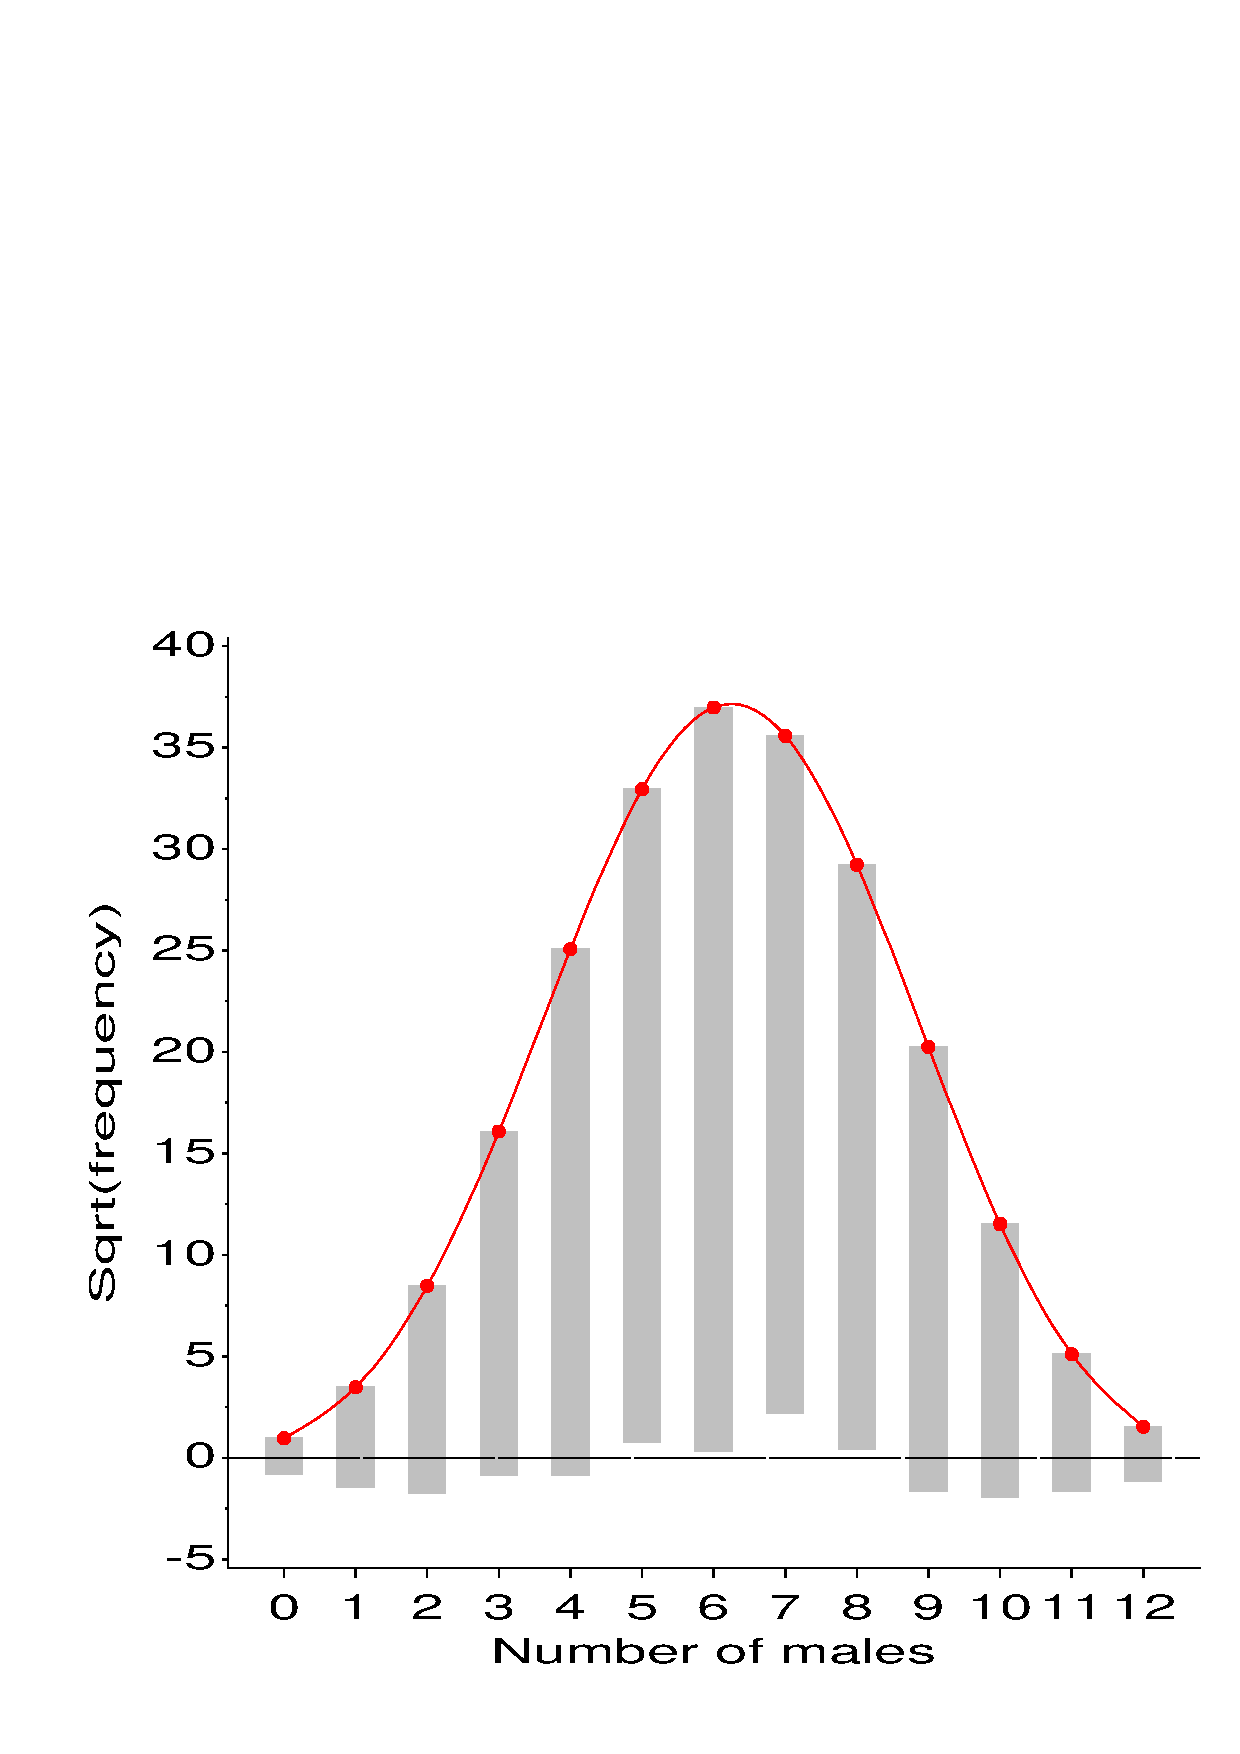
\includegraphics[width=1\linewidth]{saxony}\graphicsfile{ch2/fig/saxony.eps}{}
 \end{minipage}%
 \hfill
 \begin{minipage}[c]{.33\linewidth}
  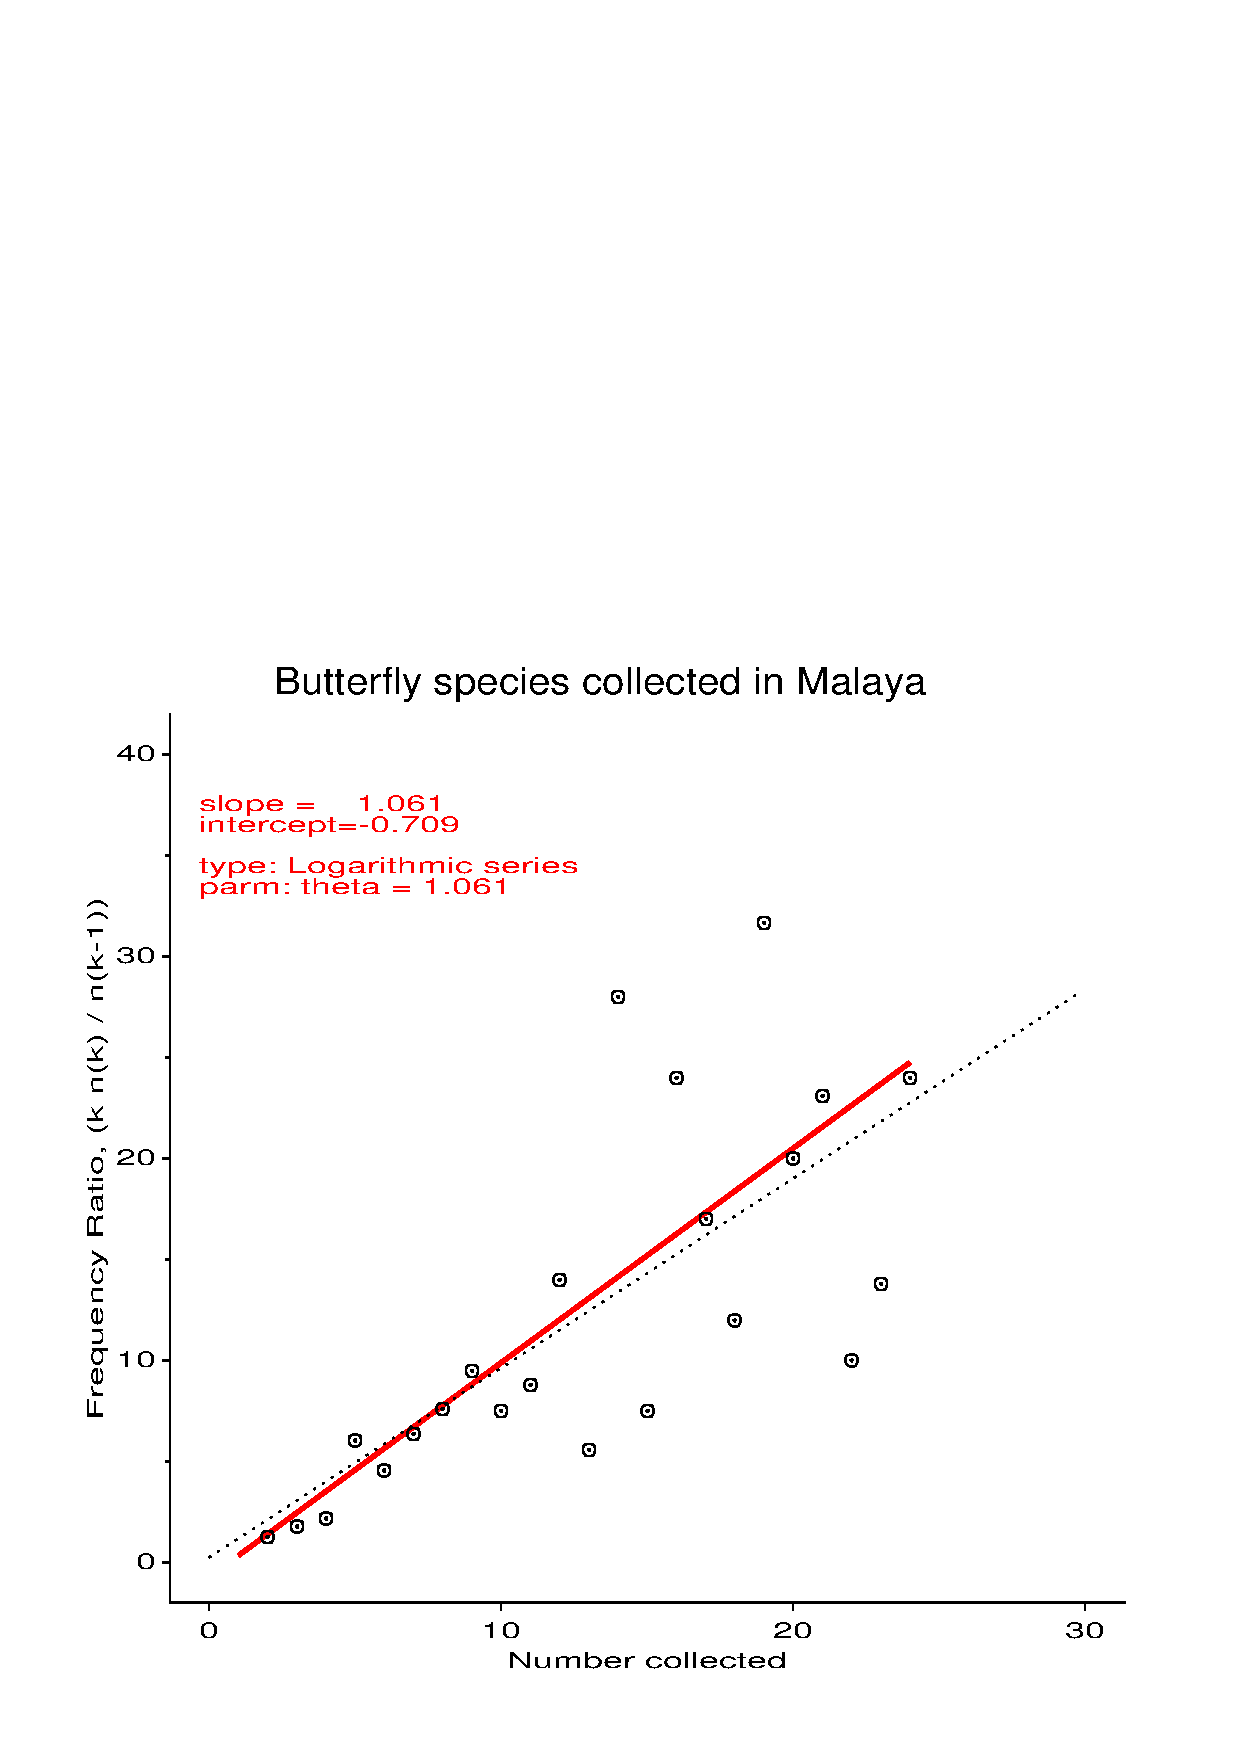
\includegraphics[width=1\linewidth]{orddemo3}\graphicsfile{ch2/fig/orddemo3.eps}{}
 \end{minipage}
 \hfill
 \begin{minipage}[c]{.33\linewidth}
  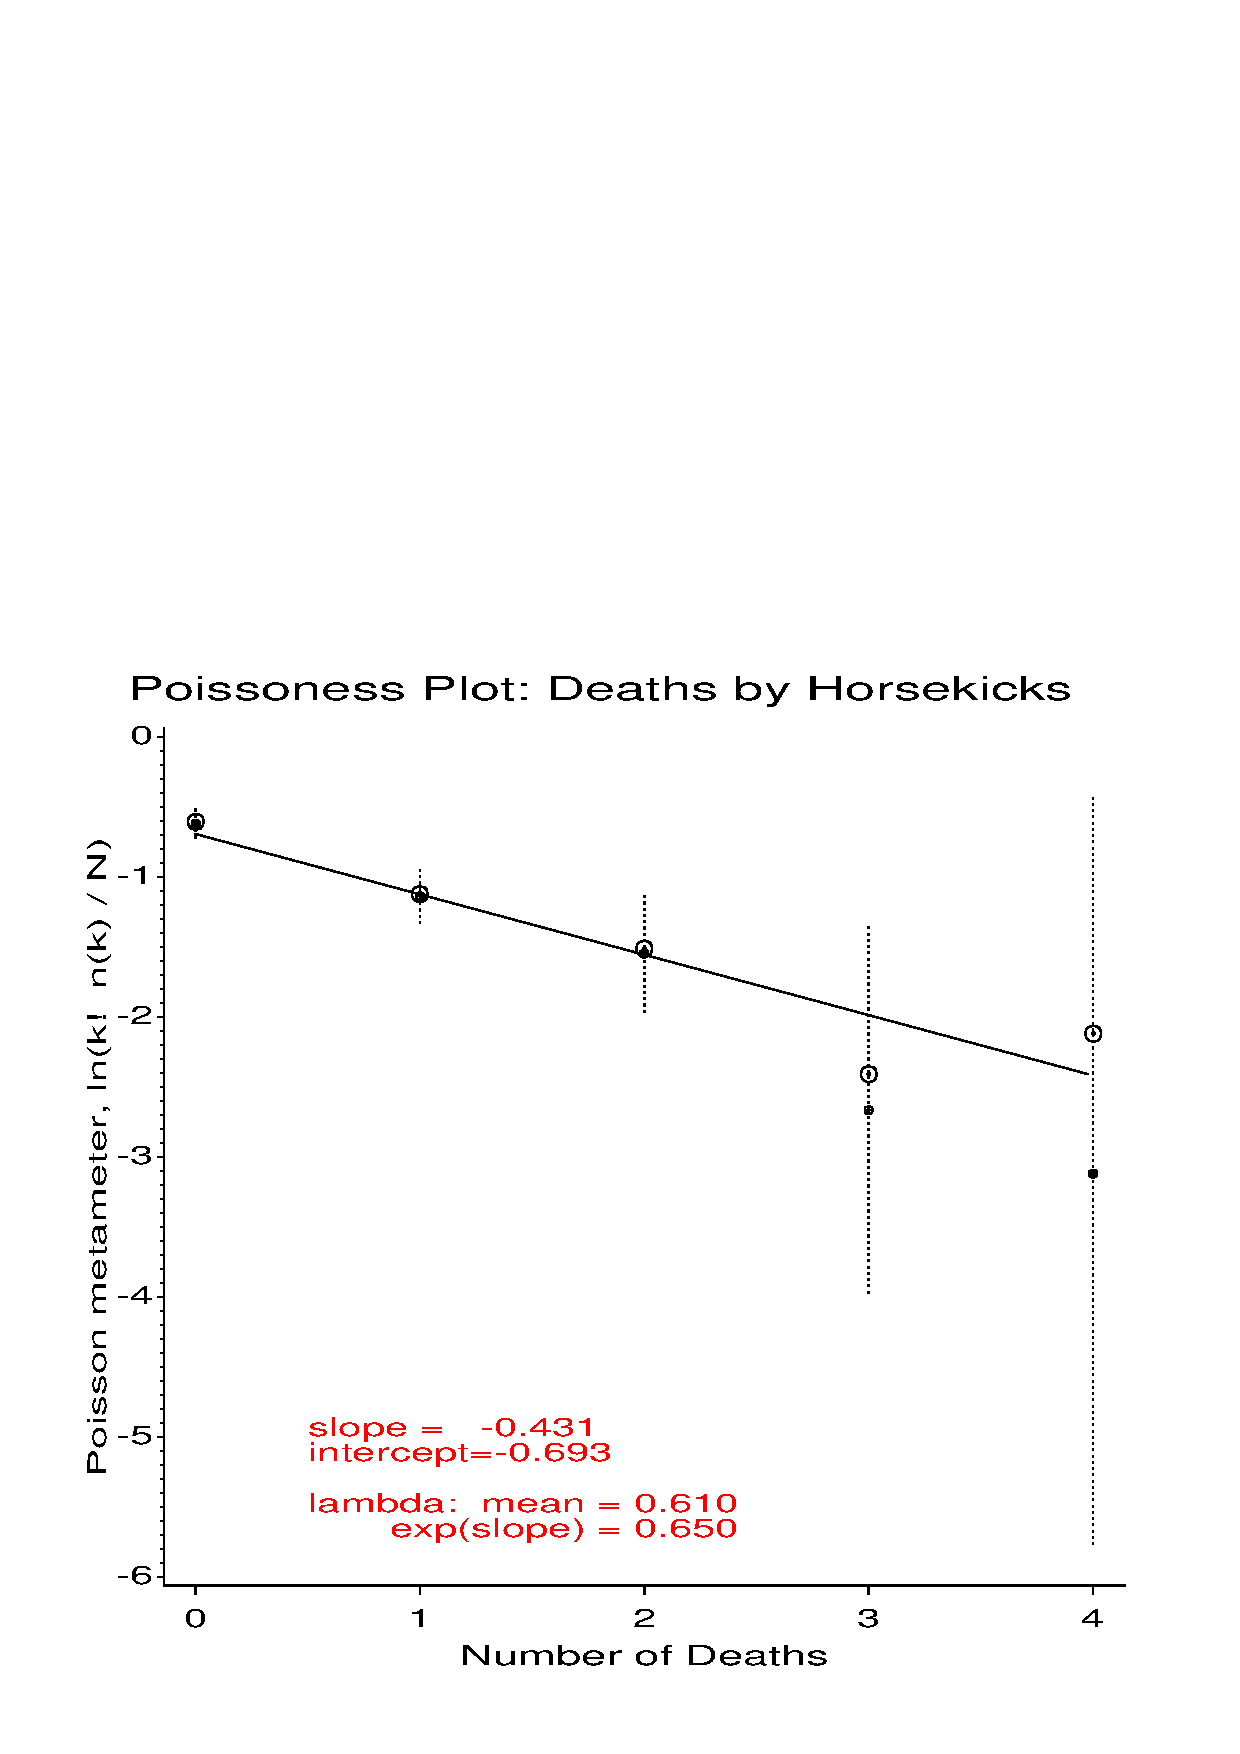
\includegraphics[width=1\linewidth]{poisdemo1}\graphicsfile{ch2/fig/poisdemo1.eps}{}
 \end{minipage}
\end{center}

   %% visual contents images

\chapterprelude{
Loglinear models comprise another special case of generalized linear models
designed for \ctabs of frequencies.  They
are most easily interpreted through
visualizations, including mosaic displays and plots of associated
logit models.  
Special cases arise for ordered categorial variables and square tables
that allow more parsimonious models for associations.
% As with logistic regression, diagnostic plots
% and influence plots help to assure that the fitted model is
% an adequate summary of associations among variables.
}
% \minitoc
% \clearpage

\section{Introduction}\label{sec:loglin-intro}

\epigraph{Tables are like cobwebs, like the
sieve of Danaides; beautifully reticulated, orderly to look upon, but
which will hold no conclusion. Tables are abstractions, and the object a most
concrete one, so difficult to read the essence of.}{From \emph{Chartism} by Thomas Carlyle (1840), Chapter II, Statistics}

The chapter continues the modeling framework begun in \chref{ch:logistic},
and takes up the case of \loglin models for contingency tables of frequencies,
when all variables are discrete, another special case of
generalized linear models.
These models provide a comprehensive scheme to describe and
understand the associations among two or more categorical variables.
Whereas logistic regression models focus on the prediction of one response factor,
\loglin models treat all variables symmetrically, and attempt to
model all important associations among them.

In this sense,
\loglin models are analogous to a correlation analysis of continuous
variables, where the goal is to determine the patterns of dependence
and independence among a set of variables.  
When one variable is a response and the others are explanatory,
certain \loglin models are equivalent to logistic models for that
response.
Such models are also particularly useful
when there are two or more response variables, a case that would require
a multivariate version of the generalized linear model, for which
the current theory and implementations are thin at best.

\chref{ch:mosaic} and \chref{ch:corresp} introduced some basic aspects of
\loglin\ models in connection with mosaic displays and correspondence analysis.
\ix{correspondence analysis}
\ix{mosaic display}
In this chapter, the focus is on fitting and interpreting
\loglin\ models.
The usual analyses, with \func{loglm} and
\func{glm}
present the results in terms of tables of parameter
estimates.  Particularly for larger tables, it becomes difficult
to understand the nature of these associations from tables
of parameter estimates.  Instead, we emphasize plots of observed
and predicted frequencies,
probabilities or log odds (when there are one or more response
variables), as well as mosaic and other displays for interpreting a given
model.
% and residual and influence plots for model diagnostics.
We also illustrate how mosaic displays and \ca plots may be used
in a complementary way to the usual numerical summaries, to provide
additional insights into the data.

\secref{sec:loglin-counts} gives a brief overview of \loglin\
models in relation to the more familiar ANOVA and regression models
for quantitative data.
Methods and software for fitting these models are discussed in
\secref{sec:loglin-fitting}.
When one variable is a response, logit models for that response provide
a simpler, but equivalent means for interpreting and graphing
results of \loglin\ models, as we describe in \secref{sec:loglin-logit}.
Another class of simplified models (\secref{sec:loglin-ordinal})
occurs when one or more of the explanatory variables are ordinal,
and discrete levels might be replaced by numerical values.
Models for square tables (\secref{sec:loglin-square}), with the same row and column categories
comprise another special case giving simpler descriptions than the saturated model of
general association. These important special cases are extended to three-way and
higher-dimensional tables in \secref{sec:loglin-3wayord}.
Finally, \secref{sec:loglin-multiv} describes some methods for dealing with situations
where there are several response variables, and it is useful to understand both
the marginal relations of the responses with the predictors as well as how their
association varies with the predictors
%\TODO{Complete Chapter overview of sections}

\section{Loglinear models for frequencies}\label{sec:loglin-counts}

\Loglin\ models have been developed from two formally distinct,
but related perspectives.  The first is a discrete analog of familiar
ANOVA models
for quantitative data, where the multiplicative relations among joint and marginal probabilities are transformed into an additive one by transforming
the counts to logarithms.
The second is an analog of regression models, where the log of the
cell frequency is modeled as a linear function of discrete predictors,
with a random component often taken as the Poisson distribution
and called \term{Poisson regression}; this approach is treated in more detail as
generalized linear models for count data in \chref{ch:glm}.

\subsection{Loglinear models as ANOVA models for frequencies}
For two discrete variables, $A$ and $B$, suppose we have a multinomial sample of $n_{ij}$ observations in each cell $i,j$ of an $I \times J$
\ctab.   To ease notation, we replace a subscript by $+$ to represent
summation over that dimension, so that $n_{i+} = \Sigma_j n_{ij}$,
$n_{+j} = \Sigma_i n_{ij}$, and $n_{++} = \Sigma_{ij} n_{ij}$.

Let $\pi_{ij}$ be the joint probabilities in the table, and let
$m_{ij} = n_{++} \pi_{ij}$ be the expected cell frequencies under
any model.
Conditional on the observed total count, $n_{++}$,
each count has a Poisson distribution, with mean $m_{ij}$.
Any \loglin\ model may be expressed as a linear model for the $\log m_{ij}$.
For
example, the hypothesis of independence means that the expected
frequencies, \(m_{ij}\), obey
\begin{equation*}%\label{eq:indep}
  m_{ij} = \frac{ m_{i+} \:  m_{+j} } {m_{++}}
  \period
\end{equation*}

This multiplicative model can be transformed to an additive (linear)
model by taking logarithms of both sides:
\begin{equation*}
  \log ( m_{ij} ) = \log ( m_{i+} )  +  \log ( m_{+j} )
 - \log ( m_{++} )
 \comma
\end{equation*}
which is usually expressed in an equivalent form in terms of model
parameters,
\begin{equation} \label{eq:lmain}
\log ( m_{ij} ) = \mu  +  \lambda_i^A +  \lambda_j^B
\end{equation}
where \(\mu\) is a function of the total sample size, \(\lambda_i^A\)
is the ``main effect'' for variable A,
\(\lambda_i^A = \log \pi_{i+} - \sum_k(\log \pi_{k+}) / I \),
 and \(\lambda_j^B\) is the
``main effect'' for variable B,
\(\lambda_j^B = \log \pi_{+j} - \sum_k(\log \pi_{+k}) / J \).
Model \eqref{eq:lmain} is called the \term{loglinear independence model}
for a two-way table.

In this model, there
are $1 + I + J$ parameters,  but only $(I-1)+(J-1)$ are separately
estimable. Hence,
the typical ANOVA sum-to-zero
restrictions
are usually applied to the parameters:
\begin{equation*}
\sum_i^I \:
\lambda_i^A  = \sum_j^J \:  \lambda_j^B = 0 \period
\end{equation*}
These ``main effects'' in
\loglin models pertain to differences among the marginal
probabilities of a variable (which are usually not of direct interest).

Other restrictions to make the parameters identifiable are also used.
Setting the first values,
$\lambda_1^A$ and $\lambda_1^B$
to zero (the default in \func{glm}), defines
$\lambda_i^A = \log \pi_{i+} - \log \pi_{1+}$, and
$\lambda_j^B = \log \pi_{+j} - \log \pi_{+1}$,
as deviations from the first, reference category,
but these parameterizations are otherwise identical.
For modeling functions in \R (\func{lm}, \func{glm}, etc.)
the reference category parameterization is obtained using
\func{contr.treatment}, while the sum-to-zero constraints
are obtained with \func{contr.sum}.

Model \eqref{eq:lmain} asserts that the row and column variables
are independent.
For a two-way table, a model that allows an arbitrary
association between the variables is the \term{saturated model},
including an additional term, $\lambda_{ij}^{AB}$:
\begin{equation}\label{eq:lsat}
\log ( m_{ij} ) = \mu  +  \lambda_i^A
+  \lambda_j^B  +  \lambda_{ij}^{AB} \comma
\end{equation}
where again, restrictions must be imposed for estimation:
\begin{equation}\label{eq:lrestrict}
\sum_i^I \,  \lambda_i^A  = 0, \quad
\sum_j^J \,  \lambda_j^B = 0, \quad
\sum_i^I \,  \lambda_{ij}^{AB} =
\sum_j^J \,  \lambda_{ij}^{AB} = 0  \period
\end{equation}
There are thus $I-1$ linearly independent $\lambda_i^A$ row parameters,
$J-1$ linearly independent $\lambda_j^B$ column parameters,
and $(I-1)(J-1)$ linearly independent $\lambda_{ij}^{AB}$ association  parameters.
This model is called the \emph{saturated model} because the number of
parameters in $\mu$, $\lambda_i^A$, $\lambda_j^B$, and $\lambda_{ij}^{AB}$
is equal to the number of frequencies in the two-way table,
\begin{equation*}
  \cwe{1}{\mu} + \cwe{I-1}{\lambda_i^A} + \cwe{J-1}{\lambda_j^B} + \cwe{(I-1)(J-1)}{\lambda_{ij}^{AB}}
  = \cwe{I J}{n_{ij}}
\end{equation*}
The association parameters $\lambda_{ij}^{AB}$ express the departures from independence,
so large absolute values pertain to cells that differ from the independence model.

Except for the difference in notation, model \eqref{eq:lsat} is formally the same
as a two-factor ANOVA model with an interaction, typically expressed as
$  E ( y_{ij} ) = \mu  +  \alpha_i  +  \beta_j +(\alpha  \beta)_{ij}
$.
Hence, associations between variables in \loglin models are
analogous to interactions in ANOVA models.
The use of superscripted symbols,
$\lambda_i^A, \lambda_j^B , \lambda_{ij}^{AB}$ rather than separate
Greek letters is a convention in \loglin models, and useful mainly
for \mway\ tables.

Models such as \eqref{eq:lmain} and \eqref{eq:lsat} are
examples of \term{hierarchical models}.
This means that the model must contain all lower-order terms contained
within any high-order term in the model.
Thus, the saturated model, \eqref{eq:lsat} contains $\lambda_{ij}^{AB}$,
and therefore \emph{must} contain $\lambda_i^A $ and $\lambda_j^B$.
As a result, hierarchical models may be identified by the shorthand
notation which lists only the high-order terms: model \eqref{eq:lsat}
is denoted $[A B]$, while model \eqref{eq:lmain} is $[A] [B]$.

\subsection{\Loglin\ models for three-way tables}\label{sec:loglin-3way}
\Loglin models for three-way \ctabs
were described briefly in \secref{sec:mosaic-fitting}.
Each type of model allows associations among different sets of variables
and each has a different independence interpretation, as illustrated in
\tabref{tab:hyp3way}.

For a three-way table, the saturated model, denoted $[ABC]$ is
\begin{equation} \label{eq:lsat3}
  \log \,  m_{ijk}  =
  \mu  +  \lambda_i^A
  +  \lambda_j^B
  +  \lambda_k^C
  +  \lambda_{ij}^{AB}
  +  \lambda_{ik}^{AC}
  +  \lambda_{jk}^{BC}
  +  \lambda_{ijk}^{ABC}
  \period
\end{equation}
This model allows all variables to be associated; \eqref{eq:lsat3} fits the data perfectly because
the number of independent parameters equals the number of table cells.
Two-way terms, such as $\lambda_{ij}^{AB}$ pertain to the
\emph{conditional association} between pairs of factors,
controlling for the remaining variable.
The presence of the three-way term, $\lambda_{ijk}^{ABC}$,
means that the partial association (conditional odds ratio) between any pair
varies over the levels of the third variable.

Omitting the three-way term in Model \eqref{eq:lsat3} gives the model
$[AB] [AC] [BC]$,
\begin{equation} \label{eq:lno3way}
  \log \,  m_{ijk}  =
  \mu  +  \lambda_i^A
  +  \lambda_j^B
  +  \lambda_k^C
  +  \lambda_{ij}^{AB}
  +  \lambda_{ik}^{AC}
  +  \lambda_{jk}^{BC}
  \comma
\end{equation}
in which all pairs are conditionally dependent given the remaining one.
For any pair,
the conditional odds ratios are the \emph{same} at all levels of the remaining
variable, so this model is often called the \term{homogeneous association model}.

The interpretation of terms in this model may be illustrated
using the Berkeley admissions data (\exref{ex:berkeley2} and \exref{ex:berkeley3}), for which the factors are Admit,
 Gender, and Department, in a $2 \times 2 \times 6$ table.
In the homogeneous association model,
\begin{equation}\label{eq:berk1}
  \log \,  m_{ijk}  =
  \mu  +  \lambda_i^A
  +  \lambda_j^D
  +  \lambda_k^G
  +  \lambda_{ij}^{AD}
  +  \lambda_{ik}^{AG}
  +  \lambda_{jk}^{DG}
  \comma
\end{equation}
the $\lambda$-parameters have the following interpretations:
\begin{itemize}
\item The main effects, $\lambda_i^A , \lambda_j^D$ and $\lambda_k^G$
   pertain to differences in the one-way marginal probabilities.
    Thus $\lambda_j^D$ relates to differences in the total number of applicants
    to these departments, while $\lambda_k^G$ relates to the differences
    in the overall numbers of men and women applicants.
\item $\lambda_{ij}^{AD}$ describes the conditional association between
   admission and department, that is  different admission rates across
   departments (controlling for gender).
\item $\lambda_{ik}^{AG}$ relates to the conditional association between
   admission and gender, controlling for department.
    This term, if significant, might be interpreted as indicating
   gender-bias in admissions.
\item $\lambda_{jk}^{DG}$, the association between
 department and gender, indicates whether males and females apply
 differentially across departments.
\end{itemize}

As we discussed earlier (\secref{sec:mosaic-threeway}), \loglin models
for three-way (and larger) tables often have an interpretation in terms
of various types of independence relations illustrated in \tabref{tab:hyp3way}.
The model \eqref{eq:lno3way} has no such interpretation, however the smaller
model $\LLM{AC, BC}$ can be interpreted as asserting that $A$ and $B$ are
(conditionally) independent controlling for $C$;  this independence interpretation
is symbolized as $A \perp B \given C$.
Similarly, the model $\LLM{AB, C}$ asserts that $A$ and $B$ are jointly
independent of $C$: $(A, B) \perp C$, while the model $\LLM{A, B, C}$
is the model of mutual (complete) independence, $A \perp B \perp C$.


\subsection{Loglinear models as GLMs for frequencies}\label{sec:loglin-glms}
In the GLM approach, a \loglin model may be cast in the form of a regression
model for $\log \vec{m}$, where the table cells are reshaped to a
column vector.
One advantage is that models for tables of any size and structure
may be expressed in a compact form.

For a contingency table of variables $A, B, C,\cdots $, with $N=I\times
J\times K\times \cdots $ cells, let $\vec{n}$ denote a column vector of
the observed counts arranged in standard order, and let $\vec{m}$ denote
a similar vector of the expected frequencies under some model. Then \emph{any}
\loglin model may be expressed
in the form
\begin{equation*}
 \log \vec{m} = \mat{X}\vec{\beta}
 \comma
\end{equation*}
where $\mat{X}$ is a known design or \term{model matrix} and $\vec{\beta}$ is a
column vector containing the unknown $\lambda $ parameters.

For example, for
a $2\times 2$ table, the saturated model \eqref{eq:lsat} with the usual zero-sum constraints \eqref{eq:lrestrict}
can be represented as
\begin{equation*}
\log \left(
\begin{array}{c}
 m_{11} \\
 m_{12} \\
 m_{21} \\
 m_{22}
\end{array}
\right) =\left[
\begin{array}{rrrr}
1 & 1 & 1 & 1 \\
1 & 1 & -1 & -1 \\
1 & -1 & 1 & -1 \\
1 & -1 & -1 & 1
\end{array}
\right] \left(
\begin{array}{c}
\mu  \\
\lambda _1^A \\
\lambda _1^B \\
\lambda _{11}^{AB}
\end{array}
\right)
\end{equation*}
Note that only the linearly independent parameters are represented here.
$\lambda_2^A = - \lambda_1^A$, because $\lambda_1^A + \lambda_2^A =0$, and
$\lambda_2^B = - \lambda_1^B$, because $\lambda_1^B + \lambda_2^B =0$,
and so forth.

An additional substantial advantage of the GLM formulation is that it makes it easier
to express models with ordinal or quantitative variables.
\func{glm}, with a model formula of the form
\verb|Freq ~ .| involving factors $A, B, \dots$ and quantitative variables
$x_1, x_2, \dots$,
constructs the model matrix $\mat{X}$ from the terms given in the formula.
A factor with $K$ levels gives rise to $K-1$ columns
for its main effect and sets of $K-1$ columns in each interaction effect.
A quantitative predictor, say $x_1$ (with a linear effect)
creates a single column with its values
and interactions with other terms are calculated at the products
of the columns for the main effects.

The parameterization for factors is controlled by
the contrasts assigned to a given factor (if any), or by the general
\code{contrasts} option, that gives the contrast functions used
for unordered and ordered factors:
\begin{knitrout}
\definecolor{shadecolor}{rgb}{1, 0.961, 0.933}\color{fgcolor}\begin{kframe}
\begin{alltt}
\hlkwd{options}\hlstd{(}\hlstr{"contrasts"}\hlstd{)}
\end{alltt}
\begin{verbatim}
## $contrasts
##         unordered           ordered 
## "contr.treatment"      "contr.poly"
\end{verbatim}
\end{kframe}
\end{knitrout}
\noindent This says that, by default, unordered factors use
the baseline (first) reference-level parameterization, while
ordered factors are given a parameterization based on orthogonal
polynomials, allowing linear, quadratic, ... effects, assuming
integer-spacing of the factor levels.



\section{Fitting and testing \loglin models} \label{sec:loglin-fitting}

For a given table, possible \loglin models range from the
baseline model of mutual independence, $\LLM{A, B, C, \dots}$
to the saturated model, $\LLM{A B C \dots}$ that fits the
observed frequencies perfectly, but offers no simpler description or
interpretation than the data itself.

Fitting a \loglin model
is usually a process of deciding which association terms are large enough
(``significantly different from zero'') to warrant inclusion
in a model to explain the observed frequencies.
Terms which are excluded from the model go
into the residual or error term, which reflects the overall
badness-of-fit of the model.  The usual goal of \loglin modeling
is to find a small model (few association terms) which nonetheless achieves a
reasonable fit (small residuals).

\subsection{Model fitting functions} \label{sec:loglin-functions}
In \R, the most basic function for fitting \loglin models is
\func{loglin} in the \Rpackage{stats}.
This uses the classical iterative proportional fitting (IPF) algorithm
described in \citet{Haberman:1972} and \citet[\S 3.4]{Fienberg:80}.
It is designed to work with the frequency data in table form,
and a model specified in terms of the (high-order) table margins
to be fitted. For example, the model \eqref{eq:lno3way}
of homogenous association for a three-way table is specified
as
\begin{knitrout}
\definecolor{shadecolor}{rgb}{1, 0.961, 0.933}\color{fgcolor}\begin{kframe}
\begin{alltt}
\hlkwd{loglin}\hlstd{(mytable,} \hlkwc{margin}\hlstd{=}\hlkwd{list}\hlstd{(}\hlkwd{c}\hlstd{(}\hlnum{1}\hlstd{,} \hlnum{2}\hlstd{),} \hlkwd{c}\hlstd{(}\hlnum{1}\hlstd{,} \hlnum{3}\hlstd{),} \hlkwd{c}\hlstd{(}\hlnum{2}\hlstd{,} \hlnum{3}\hlstd{)))}
\end{alltt}
\end{kframe}
\end{knitrout}

The function \func{loglm} in \pkg{MASS} provides a more convenient
front-end to \func{loglin}
to allow \loglin models to be specified using a model formula.
With table variables \code{A}, \code{B} and \code{C}, the same model can be
fit using \func{loglm} as
\begin{knitrout}
\definecolor{shadecolor}{rgb}{1, 0.961, 0.933}\color{fgcolor}\begin{kframe}
\begin{alltt}
\hlkwd{loglm}\hlstd{(}\hlopt{~} \hlstd{(A} \hlopt{+} \hlstd{B} \hlopt{+} \hlstd{C)}\hlopt{^}\hlnum{2}\hlstd{,} \hlkwc{data}\hlstd{=mytable)}
\end{alltt}
\end{kframe}
\end{knitrout}
When the data is a frequency data frame with frequencies in \code{Freq},
for example, the result of \code{mydf <- as.data.frame(mytable)},
you can also use a two-sided formula:
\begin{knitrout}
\definecolor{shadecolor}{rgb}{1, 0.961, 0.933}\color{fgcolor}\begin{kframe}
\begin{alltt}
\hlkwd{loglm}\hlstd{(Freq} \hlopt{~} \hlstd{(A} \hlopt{+} \hlstd{B} \hlopt{+} \hlstd{C)}\hlopt{^}\hlnum{2}\hlstd{,} \hlkwc{data}\hlstd{=mydf)}
\end{alltt}
\end{kframe}
\end{knitrout}

As implied in \secref{sec:loglin-glms}, \loglin models can also be fit
using \func{glm}, using \code{family=poisson} which constructs the
model for \code{log(Freq)}.  The same model is fit with \func{glm}
as:
\begin{knitrout}
\definecolor{shadecolor}{rgb}{1, 0.961, 0.933}\color{fgcolor}\begin{kframe}
\begin{alltt}
\hlkwd{glm}\hlstd{(Freq} \hlopt{~} \hlstd{(A} \hlopt{+} \hlstd{B} \hlopt{+} \hlstd{C)}\hlopt{^}\hlnum{2}\hlstd{,} \hlkwc{data}\hlstd{=mydf,} \hlkwc{family}\hlstd{=poisson)}
\end{alltt}
\end{kframe}
\end{knitrout}
While all of these fit equivalent models, the details of the printed output,
model objects, and available methods differ, as indicated in some of the examples
that follow.

It should be noted that both the \func{loglin}/\func{loglm} methods based
on iterative proportional fitting, and the \func{glm} approach using
the Poisson model for log frequency give maximum likelihood estimates,
$\widehat{\vec{m}}$, of the expected frequencies, as long as all
observed frequencies $\vec{n}$ are \emph{all} positive.
Some special considerations when there cells with
zero frequencies are described in \secref{sec:loglin-zeros}.


\subsection{Goodness-of-fit tests} \label{sec:loglin-goodfit}

For an \nway table, global goodness-of-fit tests for a \loglin model
attempt to answer the question ``How well does the model reproduce
the observed frequencies?'' That is, how close are the fitted frequencies
estimated under the model to those of the saturated model or the data?

To avoid multiple subscripts for an \nway table,
let $\vec{n} = n_1, n_2, \ldots , n_N$ denote
the observed frequencies in a table with $N$ cells, and
corresponding fitted frequencies
$\widehat{\vec{m}} = \widehat{m}_1, \widehat{m}_2, \ldots , \widehat{m}_N$
according to a particular \loglin model.
The standard goodness-of-fit statistics are sums over the cells
of measures of the difference between the $\vec{n}$ and $\widehat{\vec{m}}$.

The most commonly used are the familiar Pearson chi-square,
\begin{equation}\label{eq:pchi}
X^2 = \sum_i^N \frac{( n_i - \widehat{m}_i )^2}{\widehat{m}_i}
\comma
\end{equation}
and the \LR\ \GSQ\ or \term{deviance} statistic,
\begin{equation}\label{eq:pgsq}
\GSQ =  2 \sum_i^N n_i \, \log \left( \frac{n_i} {\widehat{m}_i} \right)
\period
\end{equation}
Both of these statistics have asymptotic \chisq
distributions (as $\Sigma \vec{n} \to \infty$), reasonably well-approximated
when all expected frequencies are large.%
\footnote{
% A wider class of test statistics including \chisq\
% and \GSQ\ as special cases is
% described by \citet{CressieRead:84} and \citet{ReadCressie:88}.
Except in bizarre or borderline
cases, these tests provide the same conclusions when
expected frequencies are at least moderate (all $\widehat{\vec{m}} > 5$).
However, \GSQ approaches the theoretical chi-squared distribution
more slowly than does \chisq, and the approximation may be poor
when the average cell frequency is less than 5.
}
The (residual) degrees of freedom are the number of cells ($N$) minus the
number of estimated parameters.
The \LR test can also be expressed as twice the difference
in log-likelihoods under saturated and fitted models,
\begin{equation*}%\label{eq:lrt}
% \GSQ =  -2 \log \left[ \frac{\mathcal{L}(\widehat{\vec{m}}; \vec{n})}
%                             {\mathcal{L}(\vec{n}; \vec{n})}  \right]
%      =  -2 [ \log \mathcal{L}(\widehat{\vec{m}}; \vec{n})
%            - \log \mathcal{L}(\vec{n}; \vec{n}) ]
\GSQ =  2 \log \left[ \frac{\mathcal{L}(\vec{n}; \vec{n})}  {\mathcal{L}(\widehat{\vec{m}}; \vec{n})}
               \right]
     =  2 [ 
           \log \mathcal{L}(\vec{n}; \vec{n}) 
         - \log \mathcal{L}(\widehat{\vec{m}}; \vec{n})
          ]
\comma
\end{equation*}
where 
% $\mathcal{L}(\widehat{\vec{m}}; \vec{n})$ is the maximized likelihood
% for the fitted model and 
% $\mathcal{L}(\vec{n}; \vec{n})$ is the corresponding
% likelihood for the saturated model.
% 
$\mathcal{L}(\vec{n}; \vec{n})$ is the
likelihood for the saturated model and
$\mathcal{L}(\widehat{\vec{m}}; \vec{n})$ is the corresponding maximized likelihood
for the fitted model.


In practice such global tests are less useful for comparing competing models.
You may  find that several different models have an acceptable fit
or, sadly, that none do (usually because you are ``blessed'' with a
large sample size).
It is then helpful to compare competing models \emph{directly},
and two strategies are particularly useful in these cases.

First, the \LR\ \GSQ\ statistic has the property
in that one can compare two
\term{nested models} by their difference in \GSQ statistics,
which has a \chisq distribution on the difference in degrees of
freedom.
Two models, $M_1$ and $M_2$, are nested when one, say, $M_2$, is
a special case of the other.  That is, model $M_2$ (with $\nu_2$ residual df)
contains a subset of
the parameters of $M_1$ (with $\nu_1$ residual df),
the remaining ones being effectively set to zero.
Model $M_2$ is therefore more restrictive and cannot fit the data better
than the more general model $M_1$, i.e., $\GSQ (M_2) \ge \GSQ (M_2)$.
The least restrictive of all models, with $\GSQ = 0$ and $\nu=0$ df is
the saturated model for which $\widehat{\vec{m}} = \vec{n}$.

Assuming that the less restrictive model $M_1$ fits, the difference in
\GSQ,
\begin{eqnarray}
\Delta \GSQ \equiv \GSQ ( M_2 \given M_1 )
& = & \GSQ ( M_2 ) - \GSQ ( M_1 ) \label{eq:gsqnest1} \\
& = & 2 \sum_i n_i \, \log ( \widehat{m}_{i1} / \widehat{m}_{i2} ) \label{eq:gsqnest2}
\end{eqnarray}
has a chi-squared distribution with df = $\nu_2 - \nu_1$.
The last equality \eqref{eq:gsqnest2} follows from substituting in \eqref{eq:pgsq}.

Rearranging terms in \eqref{eq:gsqnest1}, we see that we can partition
the $\GSQ ( M_2 )$ into two terms,
\begin{equation*}
\GSQ ( M_2 ) = \GSQ ( M_1 ) + \GSQ ( M_2 \given M_1 )
\period
\end{equation*}
The first term measures the difference between the data and the more
general model $M_1$.  If this model fits, the second term measures the
additional lack of fit imposed by the more restrictive model.
In addition to providing a more focused test, $\GSQ ( M_2 \given M_1 )$
also follows the chi-squared distribution more closely when some
$\{ m_i \}$ are small
\citep[\S 10.6.3]{Agresti:2013}.

Alternatively, a second strategy uses other measures that combine
goodness-of-fit with model parsimony and may also be used to compare
non-nested models.  The statistics described below are all cast in
the form of badness-of-fit relative to degrees of freedom, so that
smaller values reflect ``better'' models.

The simplest idea \citep{Goodman:71}
is to use $\GSQ / df$
(or $\chisq / df$), which has an asymptotic expected value of 1 for a good-fitting
model.  This type of measure is not routinely reported by \R software, but is
easy to calculate from output.

The \term{Akaike Information Criterion} (AIC) statistic
\ix{AIC}
\citep{Akaike:73} is a very general criterion for model selection
with maximum likelihood estimation, based on the idea of maximizing
the information provided by a fitted model.  AIC is defined generally
as
\begin{equation*}
\mbox{AIC} = -2 \log \mathcal{L} + 2 k
\end{equation*}
where $\log \mathcal{L}$ is the maximized log likelihood and $k$ is
the number of parameters estimated in the model.
Better models correspond to \emph{smaller} AIC.  For \loglin models,
minimizing AIC is equivalent to minimizing
\begin{equation*}
\mbox{AIC}^{\star} = \GSQ - 2 \, \nu \comma
\end{equation*}
where $\nu$ is the residual df,
but the values of AIC and AIC$^\star$ differ by an arbitrary constant.
This form is easier to calculate by hand
from the output of any modeling function if AIC is not reported,
or an \func{AIC} method is not available.

A third statistic of this type is the \term{Bayesian Information Criterion}
(BIC) due to \citet{Schwartz:78} and \citet{Raftery:1986},
\ix{BIC}
\begin{equation*}
\mbox{BIC} = \GSQ - \log (n) \, \nu \comma
\end{equation*}
where $n$ is the total sample size.  Both AIC and BIC penalize the fit
statistic for increasing number of parameters.
BIC also penalizes the fit directly with (log) sample size, and so expresses
a preference for less complex models than AIC as the sample size increases.

\subsection{Residuals for \loglin models}\label{sec:loglin-residuals}

Test statistics such as \GSQ can determine whether a model has significant
lack of fit, and model comparison tests using $\Delta \GSQ = \GSQ (M_2 \given M_1)$
can assess whether the extra term(s) in model $M_1$ significantly improves the model
fit.  Beyond these tests, the pattern of residuals for individual cells
offers important clues regarding the nature of lack of fit and can help suggests
associations that could be accounted for better.

As with logistic regression models (\secref{sec:logist-resids}),
several types of residuals are available for
\loglin models. For cell $i$ in the vector form of the \ctab, the
\term{raw residual} is simply the difference between the observed and fitted
frequencies, $e_i = n_i - \widehat{m}_i$.

The \term{Pearson residual} is the square root of the contribution of the cell
to the Pearson \chisq,
\begin{equation}\label{eq:reschi2}
r_i = \frac{n_i - \widehat{m}_i}{\sqrt{\widehat{m}_i}}
\end{equation}
Similarly, the \term{deviance residual} can be defined as
\begin{equation}\label{eq:resdev2}
g_i = \sign({n_i - \widehat{m}_i}) \sqrt{2 n_i \log (n_i / \widehat{m}_i) - 2 (n_i - \widehat{m}_i) }
\end{equation}

Both of these attempt to standardize the distribution of the residuals to a standard normal,
$N (0,1)$ form.  However, as pointed out by \citet{Haberman:73}, the asymptotic variance
of these is less than one (with average value $df/N$)
but, worse--- the variance decreases with $\widehat{m}_i$.
That is, residuals for cells with small expected frequencies have larger sampling variance,
as might be expected.

Consequently, Haberman suggested dividing the Pearson residual by its estimated standard
error, giving what are often called \term{adjusted residual}s.
When \loglin models are fit using the GLM approach, the adjustment
may be calculated using the leverage (``hat value''), $h_i$ to give
appropriately standardized residuals,
\begin{eqnarray*}
r_i^\star & = & r_i / \sqrt{1 - h_i} \\
g_i^\star & = & g_i / \sqrt{1 - h_i}
\end{eqnarray*}
These standardized versions are generally preferable, particularly for visualizing
model lack of fit using mosaic displays.
The reason for preferring adjusted residuals is illustrated in
\figref{fig:stres-plot}, a plot of the factors, $\sqrt{1 - h_i}$,
determining the standard errors of the residuals against the
fitted values, $\widehat{m_i}$, in the model for the
\data{UCBAdmissions} data described in \exref{ex:berkeley6} below.
The values shown in this plot are calculated as:

\begin{knitrout}
\definecolor{shadecolor}{rgb}{1, 0.961, 0.933}\color{fgcolor}\begin{kframe}
\begin{alltt}
\hlstd{berkeley} \hlkwb{<-} \hlkwd{as.data.frame}\hlstd{(UCBAdmissions)}
\hlstd{berk.glm1} \hlkwb{<-} \hlkwd{glm}\hlstd{(Freq} \hlopt{~} \hlstd{Dept} \hlopt{*} \hlstd{(Gender}\hlopt{+}\hlstd{Admit),} \hlkwc{data}\hlstd{=berkeley,} \hlkwc{family}\hlstd{=}\hlstr{"poisson"}\hlstd{)}
\hlstd{fit} \hlkwb{<-} \hlkwd{fitted}\hlstd{(berk.glm1)}
\hlstd{hat} \hlkwb{<-} \hlkwd{hatvalues}\hlstd{(berk.glm1)}
\hlstd{stderr} \hlkwb{<-} \hlkwd{sqrt}\hlstd{(}\hlnum{1}\hlopt{-}\hlstd{hat)}
\end{alltt}
\end{kframe}
\end{knitrout}
\begin{knitrout}
\definecolor{shadecolor}{rgb}{1, 0.961, 0.933}\color{fgcolor}\begin{figure}[!htbp]


\centerline{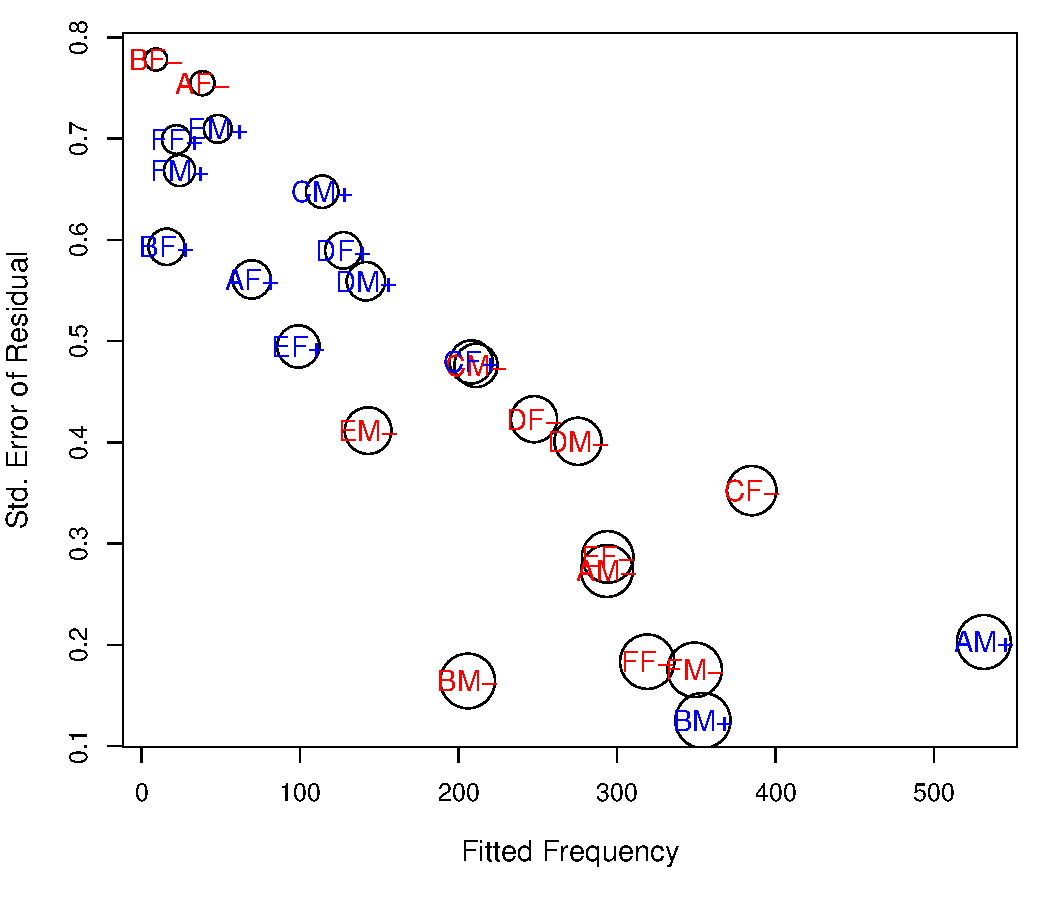
\includegraphics[width=.7\textwidth]{ch08/fig/stres-plot-1} }

\caption[Standard errors of residuals, ]{Standard errors of residuals, $\sqrt{1-h_i}$ decrease with expected frequencies. This plot shows why ordinary Pearson and deviance residuals may be misleading.  The symbol size in the plot is proportional to leverage, $h_i$. Labels abbreviate Department, Gender and Admit, colored by Admit.\label{fig:stres-plot}}
\end{figure}


\end{knitrout}


In \R, raw, Pearson and deviance residuals may be obtained using
\code{residuals(model, type=)}, where \code{type} is one of
\code{"raw"}, \code{"pearson"} and \code{"deviance"}.
Standardized (adjusted) residuals can be calculated using
\code{rstandard(model, type=)}, for \code{type="pearson"} and \code{type="deviance"}
versions.



\subsection[Using loglm()]{Using \func{loglm}}\label{loglin-loglin}
Here we illustrate the basics of fitting \loglin models using
\func{loglm}.  As indicated in \secref{sec:loglin-functions},
the model to be fitted is specified by a model formula
involving the table variables.
The \Rpackage{MASS} provides a \func{coef} method for \class{loglm} objects
that extracts the estimated parameters and a \func{residuals} method that
calculates various types of residuals according to a \code{type}
argument, one of \code{"deviance", "pearson", "response"}.
\pkg{vcd} and \pkg{vcdExtra} provide a variety of plotting methods,
including \func{assoc}, \func{sieve}, \func{mosaic} and \func{mosaic3d}
for \class{loglm} objects.


\begin{Example}[berkeley5]{Berkeley admissions}
The \data{UCBAdmissions}
on admissions to the six largest graduate departments
at U.C. Berkeley
was examined using graphical methods
in \chref{ch:twoway} (\exref{ex:berkeley3})
and in \chref{ch:mosaic} (\exref{ex:berkeley4}).
We can fit and compare several \loglin models
as shown below.

The model of mutual independence, $\LLM{A, D, G}$,
is not substantively reasonable here,
because the association of \var{Dept} and \var{Gender}
should be taken into account to control for these
variables,
but we show it here to illustrate the form of the printed output, giving
the Pearson \chisq and \LR \GSQ tests of goodness of fit,
as well as some optional arguments for saving additional
components in the result.
\begin{knitrout}
\definecolor{shadecolor}{rgb}{1, 0.961, 0.933}\color{fgcolor}\begin{kframe}
\begin{alltt}
\hlkwd{data}\hlstd{(}\hlstr{"UCBAdmissions"}\hlstd{)}
\hlkwd{library}\hlstd{(MASS)}
\hlstd{berk.loglm0} \hlkwb{<-} \hlkwd{loglm}\hlstd{(}\hlopt{~} \hlstd{Dept} \hlopt{+} \hlstd{Gender} \hlopt{+} \hlstd{Admit,} \hlkwc{data}\hlstd{=UCBAdmissions,}
                     \hlkwc{param}\hlstd{=}\hlnum{TRUE}\hlstd{,} \hlkwc{fitted}\hlstd{=}\hlnum{TRUE}\hlstd{)}
\hlstd{berk.loglm0}
\end{alltt}
\begin{verbatim}
## Call:
## loglm(formula = ~Dept + Gender + Admit, data = UCBAdmissions, 
##     param = TRUE, fitted = TRUE)
## 
## Statistics:
##                     X^2 df P(> X^2)
## Likelihood Ratio 2097.7 16        0
## Pearson          2000.3 16        0
\end{verbatim}
\end{kframe}
\end{knitrout}
The argument \code{param=TRUE} stores the estimated parameters
in the \loglin model and \code{fitted=TRUE} stores the
fitted frequencies $\widehat{m}_{ijk}$.
The fitted frequencies
can be extracted from the model object using \func{fitted}.
\begin{knitrout}
\definecolor{shadecolor}{rgb}{1, 0.961, 0.933}\color{fgcolor}\begin{kframe}
\begin{alltt}
\hlkwd{structable}\hlstd{(Dept} \hlopt{~} \hlstd{Admit}\hlopt{+}\hlstd{Gender,} \hlkwd{fitted}\hlstd{(berk.loglm0))}
\end{alltt}
\begin{verbatim}
##                 Dept      A      B      C      D      E      F
## Admit    Gender                                               
## Admitted Male        215.10 134.87 211.64 182.59 134.64 164.61
##          Female      146.68  91.97 144.32 124.51  91.81 112.25
## Rejected Male        339.63 212.95 334.17 288.30 212.59 259.91
##          Female      231.59 145.21 227.87 196.59 144.96 177.23
\end{verbatim}
\end{kframe}
\end{knitrout}

Similarly, you can extract the estimated parameters with \code{coef(berk.loglm0)},
and the Pearson residuals with \code{residuals(berk.loglm0, type="pearson")}.

Next, consider the
model of conditional independence of gender and admission given department,
$\LLM{AD, GD}$ that allows associations of admission with department and
gender with department.
\begin{knitrout}
\definecolor{shadecolor}{rgb}{1, 0.961, 0.933}\color{fgcolor}\begin{kframe}
\begin{alltt}
\hlcom{# conditional independence in UCB admissions data}
\hlstd{berk.loglm1} \hlkwb{<-} \hlkwd{loglm}\hlstd{(}\hlopt{~} \hlstd{Dept} \hlopt{*} \hlstd{(Gender} \hlopt{+} \hlstd{Admit),} \hlkwc{data}\hlstd{=UCBAdmissions)}
\hlstd{berk.loglm1}
\end{alltt}
\begin{verbatim}
## Call:
## loglm(formula = ~Dept * (Gender + Admit), data = UCBAdmissions)
## 
## Statistics:
##                     X^2 df  P(> X^2)
## Likelihood Ratio 21.736  6 0.0013520
## Pearson          19.938  6 0.0028402
\end{verbatim}
\end{kframe}
\end{knitrout}
Finally for this example, the model of homogeneous association,
$\LLM{AD, AG, GD}$ can be fit as follows.%
\footnote{It is useful to note here
that the added term $[AG]$ allows a general association of admission
with gender (controlling for department). A significance test for this term,
or for model \code{berk.loglm2} against \code{berk.loglm1}
is a proper test for the assertion of gender bias in admissions.
}
\begin{knitrout}
\definecolor{shadecolor}{rgb}{1, 0.961, 0.933}\color{fgcolor}\begin{kframe}
\begin{alltt}
\hlstd{berk.loglm2} \hlkwb{<-}\hlkwd{loglm}\hlstd{(}\hlopt{~}\hlstd{(Admit} \hlopt{+} \hlstd{Dept} \hlopt{+} \hlstd{Gender)}\hlopt{^}\hlnum{2}\hlstd{,} \hlkwc{data}\hlstd{=UCBAdmissions)}
\hlstd{berk.loglm2}
\end{alltt}
\begin{verbatim}
## Call:
## loglm(formula = ~(Admit + Dept + Gender)^2, data = UCBAdmissions)
## 
## Statistics:
##                     X^2 df  P(> X^2)
## Likelihood Ratio 20.204  5 0.0011441
## Pearson          18.823  5 0.0020740
\end{verbatim}
\end{kframe}
\end{knitrout}

Neither of these models fits particularly well, as judged by the goodness-of-fit
Pearson \chisq and \LR \GSQ test against the saturated model.
The \func{anova} method for a nested collection of \class{loglm} models
gives a series of \LR tests of the difference, $\Delta \GSQ$
between each sequential pair of models according to \eqref{eq:gsqnest1}.

\begin{knitrout}
\definecolor{shadecolor}{rgb}{1, 0.961, 0.933}\color{fgcolor}\begin{kframe}
\begin{alltt}
\hlkwd{anova}\hlstd{(berk.loglm0, berk.loglm1, berk.loglm2,} \hlkwc{test}\hlstd{=}\hlstr{"Chisq"}\hlstd{)}
\end{alltt}
\begin{verbatim}
## LR tests for hierarchical log-linear models
## 
## Model 1:
##  ~Dept + Gender + Admit 
## Model 2:
##  ~Dept * (Gender + Admit) 
## Model 3:
##  ~(Admit + Dept + Gender)^2 
## 
##           Deviance df Delta(Dev) Delta(df) P(> Delta(Dev)
## Model 1   2097.671 16                                    
## Model 2     21.736  6  2075.9357        10        0.00000
## Model 3     20.204  5     1.5312         1        0.21593
## Saturated    0.000  0    20.2043         5        0.00114
\end{verbatim}
\end{kframe}
\end{knitrout}
The conclusion from these results is that
the model \code{berk.loglm1}
is not much worse than model \code{berk.loglm2}, but there is still significant
lack-of-fit.  The next example, using \func{glm}, shows how to visualize the
lack of fit and account for it.

\end{Example}

\subsection[Using glm()]{Using \func{glm}}\label{sec:loglin-glm}
\Loglin models fit with \func{glm} require the data in a data frame
in frequency form, for example as produced by \func{as.data.frame} from
a table.
The model formula expresses the model for the frequency variable, and
uses \code{family=poisson} to specify the error distribution.
More general distributions for frequency data are discussed in
\chref{ch:glm}.

\begin{Example}[berkeley6]{Berkeley admissions}

For the $2 \times 2 \times 6$ \data{UCBAdmissions} table,
first transform this to a frequency data frame:
\begin{knitrout}
\definecolor{shadecolor}{rgb}{1, 0.961, 0.933}\color{fgcolor}\begin{kframe}
\begin{alltt}
\hlstd{berkeley} \hlkwb{<-} \hlkwd{as.data.frame}\hlstd{(UCBAdmissions)}
\hlkwd{head}\hlstd{(berkeley)}
\end{alltt}
\begin{verbatim}
##      Admit Gender Dept Freq
## 1 Admitted   Male    A  512
## 2 Rejected   Male    A  313
## 3 Admitted Female    A   89
## 4 Rejected Female    A   19
## 5 Admitted   Male    B  353
## 6 Rejected   Male    B  207
\end{verbatim}
\end{kframe}
\end{knitrout}

Then, the model of conditional independence
corresponding to \code{berk.loglm1} can be fit using \func{glm}
as shown below.
\begin{knitrout}
\definecolor{shadecolor}{rgb}{1, 0.961, 0.933}\color{fgcolor}\begin{kframe}
\begin{alltt}
\hlstd{berk.glm1} \hlkwb{<-} \hlkwd{glm}\hlstd{(Freq} \hlopt{~} \hlstd{Dept} \hlopt{*} \hlstd{(Gender}\hlopt{+}\hlstd{Admit),}
                 \hlkwc{data}\hlstd{=berkeley,} \hlkwc{family}\hlstd{=}\hlstr{"poisson"}\hlstd{)}
\end{alltt}
\end{kframe}
\end{knitrout}
Similarly, the all two-way model of homogeneous association is fit using
\begin{knitrout}
\definecolor{shadecolor}{rgb}{1, 0.961, 0.933}\color{fgcolor}\begin{kframe}
\begin{alltt}
\hlstd{berk.glm2} \hlkwb{<-} \hlkwd{glm}\hlstd{(Freq} \hlopt{~} \hlstd{(Dept} \hlopt{+} \hlstd{Gender} \hlopt{+} \hlstd{Admit)}\hlopt{^}\hlnum{2}\hlstd{,}
                 \hlkwc{data}\hlstd{=berkeley,} \hlkwc{family}\hlstd{=}\hlstr{"poisson"}\hlstd{)}
\end{alltt}
\end{kframe}
\end{knitrout}
These models are equivalent to those fit using \func{loglm} in \exref{ex:berkeley5}.
We get the same residual \GSQ as before, and the \LR test of $\Delta \GSQ$ given
by \func{anova} gives the same result, that the model \code{berk.glm2}
offers no significant improvement over model \code{berk.glm1}.

\begin{knitrout}
\definecolor{shadecolor}{rgb}{1, 0.961, 0.933}\color{fgcolor}\begin{kframe}
\begin{alltt}
\hlkwd{anova}\hlstd{(berk.glm1, berk.glm2,} \hlkwc{test}\hlstd{=}\hlstr{"Chisq"}\hlstd{)}
\end{alltt}
\begin{verbatim}
## Analysis of Deviance Table
## 
## Model 1: Freq ~ Dept * (Gender + Admit)
## Model 2: Freq ~ (Dept + Gender + Admit)^2
##   Resid. Df Resid. Dev Df Deviance Pr(>Chi)
## 1         6       21.7                     
## 2         5       20.2  1     1.53     0.22
\end{verbatim}
\end{kframe}
\end{knitrout}

Among other advantages of using \func{glm} as opposed to \func{loglm} is that
an \func{anova} method is available for \emph{individual} \class{glm} models, giving
significance tests of the contributions of each \emph{term} in the model,
as opposed to the tests for individual coefficients provided by \func{summary}.%
\footnote{
Unfortunately, in the historical development of \R, the \func{anova} methods for
linear and generalized linear
models provide only \emph{sequential} (``Type I'') tests that are computationally easy,
but useful only under special circumstances.  The \Rpackage{car} provides
an analogous \func{Anova} method that gives more generally useful
\emph{partial} (``Type II'') tests
for the additional contribution of each term beyond the others,
taking marginal relations into account.
}
\begin{knitrout}
\definecolor{shadecolor}{rgb}{1, 0.961, 0.933}\color{fgcolor}\begin{kframe}
\begin{alltt}
\hlkwd{anova}\hlstd{(berk.glm1,} \hlkwc{test}\hlstd{=}\hlstr{"Chisq"}\hlstd{)}
\end{alltt}
\begin{verbatim}
## Analysis of Deviance Table
## 
## Model: poisson, link: log
## 
## Response: Freq
## 
## Terms added sequentially (first to last)
## 
## 
##             Df Deviance Resid. Df Resid. Dev Pr(>Chi)    
## NULL                           23       2650             
## Dept         5      160        18       2491   <2e-16 ***
## Gender       1      163        17       2328   <2e-16 ***
## Admit        1      230        16       2098   <2e-16 ***
## Dept:Gender  5     1221        11        877   <2e-16 ***
## Dept:Admit   5      855         6         22   <2e-16 ***
## ---
## Signif. codes:  0 '***' 0.001 '**' 0.01 '*' 0.05 '.' 0.1 ' ' 1
\end{verbatim}
\end{kframe}
\end{knitrout}

We proceed to consider what is wrong with these models and how they can be improved.
A mosaic display can help diagnose the reason(s) for lack of fit of these models.
We focus here on the model $\LLM{AD, GD}$ that allows an association between
gender and department (i.e., men and women apply at different rates to departments).

The \func{mosaic} method for \class{glm} objects in \pkg{vcdExtra}
provides a \code{residuals\_type} argument, allowing \code{residuals\_type="rstandard"}
for standardized residuals.  The \code{formula} argument here
pertains to the order of the variables in the mosaic, not a model formula.
\begin{knitrout}
\definecolor{shadecolor}{rgb}{1, 0.961, 0.933}\color{fgcolor}\begin{kframe}
\begin{alltt}
\hlkwd{library}\hlstd{(vcdExtra)}
\hlkwd{mosaic}\hlstd{(berk.glm1,} \hlkwc{shade}\hlstd{=}\hlnum{TRUE}\hlstd{,} \hlkwc{formula}\hlstd{=}\hlopt{~}\hlstd{Admit}\hlopt{+}\hlstd{Dept}\hlopt{+}\hlstd{Gender,}
       \hlkwc{residuals_type}\hlstd{=}\hlstr{"rstandard"}\hlstd{,} \hlkwc{labeling}\hlstd{=labeling_residuals,}
       \hlkwc{main}\hlstd{=}\hlstr{"Model: [AdmitDept][GenderDept]"}\hlstd{)}
\end{alltt}
\end{kframe}\begin{figure}[!htb]


\centerline{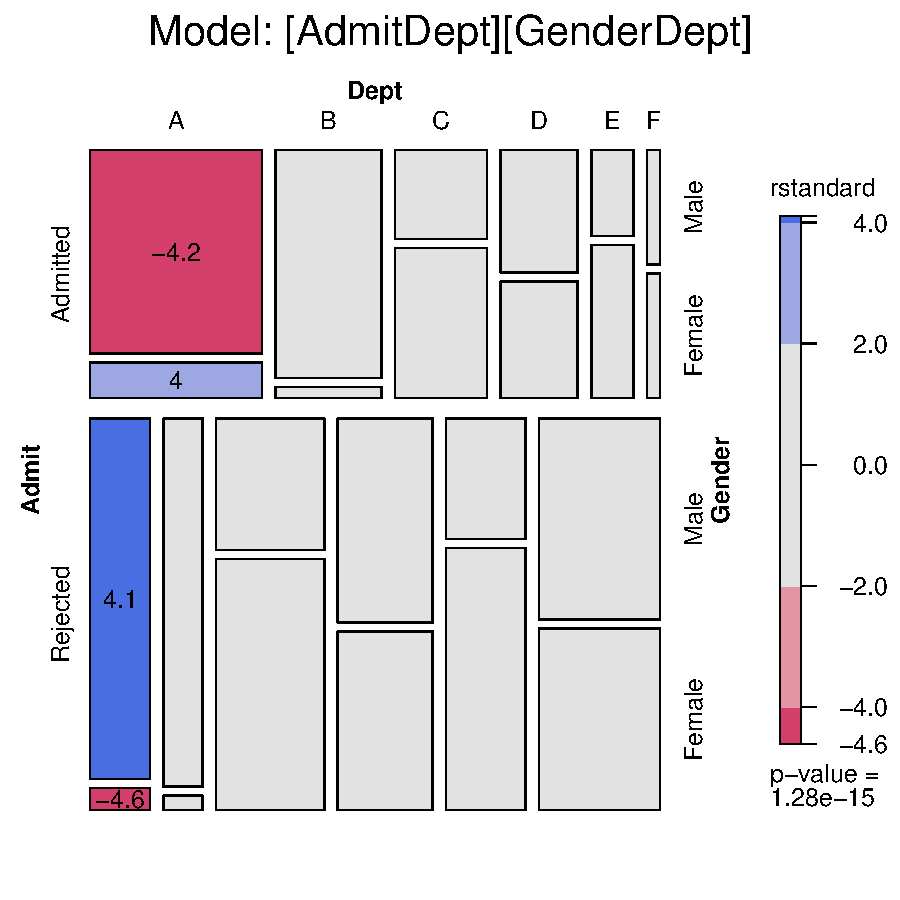
\includegraphics[width=.7\textwidth]{ch08/fig/berk-glm1-mosaic-1} }

\caption[Mosaic display for the model AD GD, showing standardized residuals]{Mosaic display for the model [AD][GD], showing standardized residuals for the cell contributions to \GSQ\label{fig:berk-glm1-mosaic}}
\end{figure}


\end{knitrout}
The mosaic display, shown in \figref{fig:berk-glm1-mosaic}, indicates that this model fits well
(residuals are small) except in Department A.
This suggests a model which allows an association between Admission and Gender in Department
A only,
\begin{equation}\label{eq:berk2}
  \log \,  m_{ijk}  =
  \mu
  +  \lambda_i^A
  +  \lambda_j^D
  +  \lambda_k^G
  +  \lambda_{ij}^{AD}
  +  \lambda_{jk}^{DG}
  +  I(j=1) \lambda_{ik}^{AG} \comma
\end{equation}
where the indicator function
$I(j=1) $ equals 1 for Department A ($j=1$) and is zero otherwise.
This model asserts that Admission and Gender are conditionally independent,
given Department, except in Department A.  It has one more parameter than
the conditional independence model, $[AD] [GD]$, and forces perfect fit
in the four cells for Department A.

Model \eqref{eq:berk2} may be fit with \func{glm} by constructing a variable
equal to the interaction of \var{gender} and \var{admit}
with a dummy variable having the value 1 for Department A and 0 for other departments.
\begin{knitrout}
\definecolor{shadecolor}{rgb}{1, 0.961, 0.933}\color{fgcolor}\begin{kframe}
\begin{alltt}
\hlstd{berkeley} \hlkwb{<-} \hlkwd{within}\hlstd{(berkeley,}
                   \hlstd{dept1AG} \hlkwb{<-} \hlstd{(Dept}\hlopt{==}\hlstr{'A'}\hlstd{)}\hlopt{*}\hlstd{(Gender}\hlopt{==}\hlstr{'Female'}\hlstd{)}\hlopt{*}\hlstd{(Admit}\hlopt{==}\hlstr{'Admitted'}\hlstd{))}
\hlkwd{head}\hlstd{(berkeley)}
\end{alltt}
\begin{verbatim}
##      Admit Gender Dept Freq dept1AG
## 1 Admitted   Male    A  512       0
## 2 Rejected   Male    A  313       0
## 3 Admitted Female    A   89       1
## 4 Rejected Female    A   19       0
## 5 Admitted   Male    B  353       0
## 6 Rejected   Male    B  207       0
\end{verbatim}
\end{kframe}
\end{knitrout}
Fitting this model with the extra term \code{dept1AG} gives \code{berk.glm3}
\begin{knitrout}\footnotesize
\definecolor{shadecolor}{rgb}{1, 0.961, 0.933}\color{fgcolor}\begin{kframe}
\begin{alltt}
\hlstd{berk.glm3} \hlkwb{<-} \hlkwd{glm}\hlstd{(Freq} \hlopt{~} \hlstd{Dept} \hlopt{*} \hlstd{(Gender}\hlopt{+}\hlstd{Admit)} \hlopt{+} \hlstd{dept1AG,}
                 \hlkwc{data}\hlstd{=berkeley,} \hlkwc{family}\hlstd{=}\hlstr{"poisson"}\hlstd{)}
\end{alltt}
\end{kframe}
\end{knitrout}
This model does indeed fit well, and represents a substantial improvement
over model \code{berk.glm1}:
\begin{knitrout}
\definecolor{shadecolor}{rgb}{1, 0.961, 0.933}\color{fgcolor}\begin{kframe}
\begin{alltt}
\hlstd{vcdExtra::}\hlkwd{Summarise}\hlstd{(berk.glm3)}
\end{alltt}
\begin{verbatim}
## Likelihood summary table:
##           AIC BIC LR Chisq Df Pr(>Chisq)
## berk.glm3 200 222     2.68  5       0.75
\end{verbatim}
\begin{alltt}
\hlkwd{anova}\hlstd{(berk.glm1, berk.glm3,} \hlkwc{test}\hlstd{=}\hlstr{"Chisq"}\hlstd{)}
\end{alltt}
\begin{verbatim}
## Analysis of Deviance Table
## 
## Model 1: Freq ~ Dept * (Gender + Admit)
## Model 2: Freq ~ Dept * (Gender + Admit) + dept1AG
##   Resid. Df Resid. Dev Df Deviance Pr(>Chi)    
## 1         6      21.74                         
## 2         5       2.68  1     19.1  1.3e-05 ***
## ---
## Signif. codes:  0 '***' 0.001 '**' 0.01 '*' 0.05 '.' 0.1 ' ' 1
\end{verbatim}
\end{kframe}
\end{knitrout}
The parameter estimate for the \code{dept1AG} term,
$\widehat{\lambda}_{ik}^{AG} = 1.052$ may be interpreted as
the log odds ratio of admission for females as compared to males in Dept. A.
The odds ratio is $\exp(1.052) = 2.86$, the same as the value calculated from the
raw data (see \secref{sec:twoway-fourstrat}).
\begin{knitrout}
\definecolor{shadecolor}{rgb}{1, 0.961, 0.933}\color{fgcolor}\begin{kframe}
\begin{alltt}
\hlkwd{coef}\hlstd{(berk.glm3)[[}\hlstr{"dept1AG"}\hlstd{]]}
\end{alltt}
\begin{verbatim}
## [1] 1.0521
\end{verbatim}
\begin{alltt}
\hlkwd{exp}\hlstd{(}\hlkwd{coef}\hlstd{(berk.glm3)[[}\hlstr{"dept1AG"}\hlstd{]])}
\end{alltt}
\begin{verbatim}
## [1] 2.8636
\end{verbatim}
\end{kframe}
\end{knitrout}
Finally, \figref{fig:berk-glm3-mosaic} shows the mosaic for this revised model.
The absence of shading indicates a well-fitting model.
\begin{knitrout}
\definecolor{shadecolor}{rgb}{1, 0.961, 0.933}\color{fgcolor}\begin{kframe}
\begin{alltt}
\hlkwd{mosaic}\hlstd{(berk.glm3,} \hlkwc{shade}\hlstd{=}\hlnum{TRUE}\hlstd{,} \hlkwc{formula}\hlstd{=}\hlopt{~}\hlstd{Admit}\hlopt{+}\hlstd{Dept}\hlopt{+}\hlstd{Gender,}
       \hlkwc{residuals_type}\hlstd{=}\hlstr{"rstandard"}\hlstd{,} \hlkwc{labeling}\hlstd{=labeling_residuals,}
       \hlkwc{main}\hlstd{=}\hlstr{"Model: [DeptGender][DeptAdmit] + DeptA*[GA]"}\hlstd{)}
\end{alltt}
\end{kframe}\begin{figure}[!htb]


\centerline{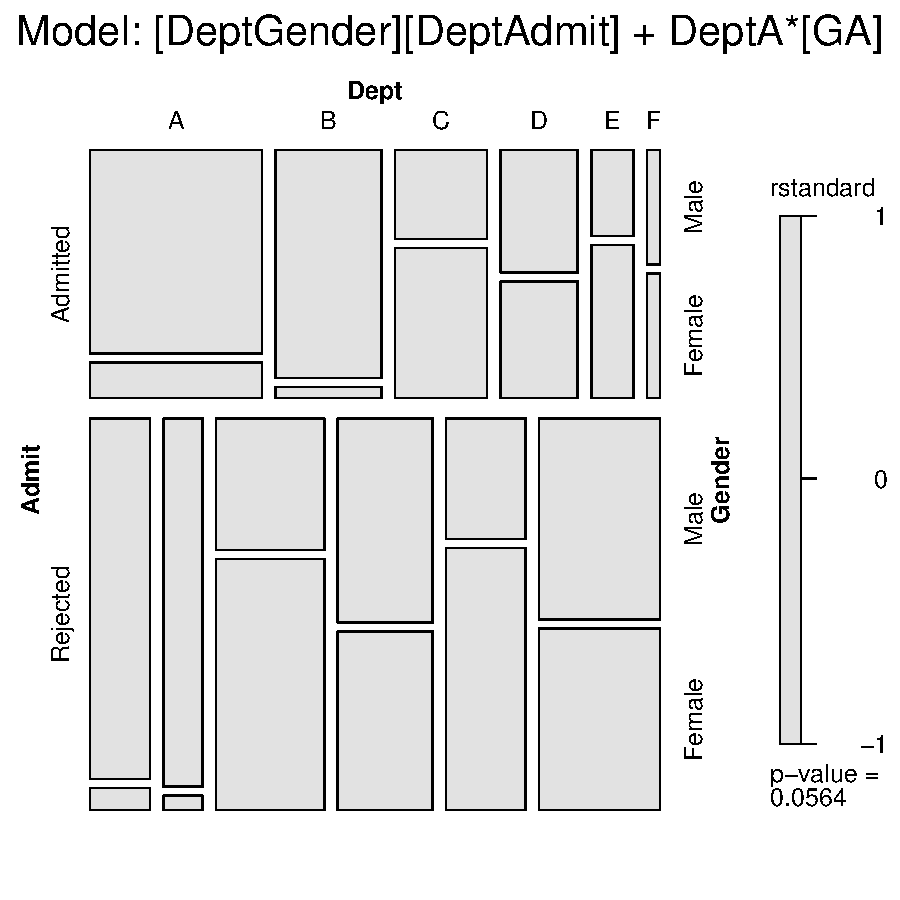
\includegraphics[width=.7\textwidth]{ch08/fig/berk-glm3-mosaic-1} }

\caption[Mosaic display for the model berk.glm3]{Mosaic display for the model \code{berk.glm3}, allowing an association of gender and admission in Department A. This model now fits the data well.\label{fig:berk-glm3-mosaic}}
\end{figure}


\end{knitrout}

\end{Example}


%\section{Two-way tables}\label{sec:loglin-twoway}
\section{Equivalent logit models}\label{sec:loglin-logit}

Because \loglin models are  formulated as models for the
log (expected) frequency, they make no distinction between
response and explanatory variables.
In effect, they treat all variables as responses
and describe their associations.

Logit (logistic regression) models, on the other hand,
describe how the log odds for one variable depends on other,
explanatory variables.
There is a close connection between the two:
When there is a response variable, each logit model for that response
is equivalent to a \loglin model.

This relationship often provides a simpler way to formulate and test
the model, and to plot and interpret the fitted results.
Even when there is no response variable, the logit representation
for one variable helps to interpret a \loglin model in terms of
odds ratios.
The price paid for this simplicity is that associations among the
explanatory variables are not expressed in the model.

Consider, for example, the model of homogeneous association, $\LLM{AB,AC,BC}$,
\eqref{eq:lno3way} for a three-way table, and let variable $C$
be a binary response.  Under this model, the logit for variable $C$
is
\begin{eqnarray*}
  L_{ij}  =
  \log \left(  \frac{\pi_{ij|1}}{\pi_{ij|2}} \right) & = &
  \log \left(  \frac{m_{ij1}}{m_{ij2}} \right) \\
    &  = &
  \log (m_{ij1}) - \log (m_{ij2})
  \period
\end{eqnarray*}
Substituting from \eqref{eq:lno3way}, all terms which do not
involve variable $C$ cancel, and we are left with
\begin{eqnarray} \label{eq:logitab1}
  L_{ij}  =
  \log ( m_{ij1} /  m_{ij2} )  & = &
  ( \lambda_1^C - \lambda_2^C )  +
  ( \lambda_{i1}^{AC} - \lambda_{i2}^{AC} )  +
  ( \lambda_{j1}^{BC} - \lambda_{j2}^{BC} )  \nonumber \\
  &  = &
  2 \lambda_1^C   +   2 \lambda_{i1}^{AC} +   2 \lambda_{j1}^{BC} \comma
\end{eqnarray}
because all \(\lambda\) terms sum  to zero.  We are interested in how these
logits depend on $A$ and $B$, so we can simplify the notation by
replacing the $\lambda$ parameters
with more familiar ones,
 \(\alpha  = 2
\lambda_1^C\), \(\beta _i^A = 2 \lambda_{i1}^{AC}\), etc., which express this relation more directly,
\begin{equation}\label{eq:logitab2}
  L_{ij}  =
  \alpha   +  \beta _i^A +  \beta _j^B
  \period
\end{equation}
In the logit model \eqref{eq:logitab2}, the response, $C$, is affected
by both $A$ and $B$, which have additive effects on the log odds of response
category $C_1$ compared to $C_2$.
The terms $\beta _i^A$ and  $\beta _j^B$
correspond directly to $[AC]$ and $[BC]$ in the \loglin\ model \eqref{eq:lno3way}. The association among the explanatory variables,
$[AB]$ is assumed in the logit model, but this model provides no explicit
representation of that association.  The logit model \eqref{eq:logitab1}
is equivalent to the \loglin\ model $[AB] [AC] [BC]$ in goodness-of-fit
and fitted values, and parameters in the two models correspond directly.

\begin{table}[!htb]
 \caption{Equivalent loglinear and logit models for a three-way table, with $C$ as
  a binary response variable}\label{tab:loglin-logit}
\centering
\begin{tabular}{lll}
\hline
Loglinear model  & Logit model           & Logit formula  \\
\hline
$\LLM{AB,C}$     & $\alpha$              & \verb| C ~ 1 | \\
$\LLM{AB,AC}$    & $\alpha + \beta_i^A$  & \verb| C ~ A | \\
$\LLM{AB,BC}$    & $\alpha + \beta_j^B$  & \verb| C ~ B | \\
$\LLM{AB,AC,BC}$ & $\alpha + \beta_i^A + \beta_j^B$  & \verb| C ~ A + B | \\
$\LLM{ABC}$      & $\alpha + \beta_i^A + \beta_j^B + \beta_{ij}^{AB}$  & \verb| C ~ A * B | \\
\hline
\end{tabular}
\end{table}
\tabref{tab:loglin-logit} shows the equivalent relationships between all
\loglin and logit models for a three-way table when variable $C$ is a binary
response.  Each model necessarily includes the $\llmterm{AB}$ association
involving the predictor variables. The most basic model, $\LLM{AB,C}$,
is the intercept-only model, asserting constant odds for variable $C$.
The saturated \loglin model $\LLM{ABC}$, allows an interaction in the
effects of $A$ and $B$ on $C$, meaning that the $AC$ association or
odds ratio varies with $B$.

More generally, when there is a binary response variable, say $R$, and
one or more explanatory variables, $A, B, C, \dots$, any logit model
for $R$ has an equivalent \loglin form.
Every term in the logit model, such as $\beta_{ik}^{AC}$, corresponds to
an association of those factors with $R$, that is, $[ACR]$ in the
equivalent \loglin\ model.

The equivalent \loglin model must also include all
associations among the explanatory factors, the term $[A B C \dots]$.
Conversely, any \loglin model which includes all associations among
the explanatory variables has an equivalent logit form.
When the response factor has more than two categories, models for
generalized logits (\secref{sec:genlogit}) also
have an equivalent \loglin form.

\begin{Example}[berkeley7]{Berkeley admissions}
The homogeneous association model, $[AD] [AG] [DG]$
did not fit the \data{UCBadmissions} data very well,
and we saw that the term $[AG]$ was unnecessary.
Nevertheless, it is instructive to consider the equivalent logit model.
We illustrate the features of the logit model which lead to the same
conclusions and simplified interpretation from graphical displays.

Because Admission
is a binary response variable, model \eqref{eq:berk1} is equivalent
to the logit model,
\begin{equation}\label{eq:berk3}
  L_{ij} =
  \log \left(
  \frac{m_{ \mbox{\scriptsize{Admit}} (ij) }} {m_{ \mbox{\scriptsize{Reject}} (ij) }}
  \right)
  =
  \alpha   +  \beta _i^{\mbox{\scriptsize Dept}}
  +  \beta _j^{\mbox{\scriptsize Gender}}
  \period
\end{equation}
That is, the logit model \eqref{eq:berk3} asserts that department and
gender have additive effects on the log odds of admission.
A significance test for the term $\beta _j^{\mbox{\scriptsize Gender}}$
here is equivalent to the test
of the $[AG]$ term for gender bias in the \loglin model.
The observed log odds of admission here can be calculated as:
\begin{knitrout}
\definecolor{shadecolor}{rgb}{1, 0.961, 0.933}\color{fgcolor}\begin{kframe}
\begin{alltt}
\hlstd{(obs} \hlkwb{<-} \hlkwd{log}\hlstd{(UCBAdmissions[}\hlnum{1}\hlstd{,,]} \hlopt{/} \hlstd{UCBAdmissions[}\hlnum{2}\hlstd{,,]))}
\end{alltt}
\begin{verbatim}
##         Dept
## Gender        A      B       C      D      E      F
##   Male   0.4921 0.5337 -0.5355 -0.704 -0.957 -2.770
##   Female 1.5442 0.7538 -0.6604 -0.622 -1.157 -2.581
\end{verbatim}
\end{kframe}
\end{knitrout}


With the data in the form of the frequency data frame \code{berkeley}
we used in \exref{ex:berkeley6}, the logit model \eqref{eq:berk3}
can be fit using \func{glm} as shown below.  In the model formula,
the binary response is \code{Admit=="Admitted"}. The \code{weights}
argument gives the frequency, \code{Freq} in each table cell.
\TODO{This gives the same fitted values, but not the same LR tests. Why?}

\begin{knitrout}
\definecolor{shadecolor}{rgb}{1, 0.961, 0.933}\color{fgcolor}\begin{kframe}
\begin{alltt}
\hlstd{berk.logit2} \hlkwb{<-} \hlkwd{glm}\hlstd{(Admit}\hlopt{==}\hlstr{"Admitted"} \hlopt{~} \hlstd{Dept} \hlopt{+} \hlstd{Gender,}
                   \hlkwc{data}\hlstd{=berkeley,} \hlkwc{weights}\hlstd{=Freq,} \hlkwc{family}\hlstd{=}\hlstr{"binomial"}\hlstd{)}
\hlkwd{summary}\hlstd{(berk.logit2)}
\end{alltt}
\begin{verbatim}
## 
## Call:
## glm(formula = Admit == "Admitted" ~ Dept + Gender, family = "binomial", 
##     data = berkeley, weights = Freq)
## 
## Deviance Residuals: 
##     Min       1Q   Median       3Q      Max  
## -25.342  -13.058   -0.163   16.017   21.320  
## 
## Coefficients:
##              Estimate Std. Error z value Pr(>|z|)    
## (Intercept)    0.5821     0.0690    8.44   <2e-16 ***
## DeptB         -0.0434     0.1098   -0.40     0.69    
## DeptC         -1.2626     0.1066  -11.84   <2e-16 ***
## DeptD         -1.2946     0.1058  -12.23   <2e-16 ***
## DeptE         -1.7393     0.1261  -13.79   <2e-16 ***
## DeptF         -3.3065     0.1700  -19.45   <2e-16 ***
## GenderFemale   0.0999     0.0808    1.24     0.22    
## ---
## Signif. codes:  0 '***' 0.001 '**' 0.01 '*' 0.05 '.' 0.1 ' ' 1
## 
## (Dispersion parameter for binomial family taken to be 1)
## 
##     Null deviance: 6044.3  on 23  degrees of freedom
## Residual deviance: 5187.5  on 17  degrees of freedom
## AIC: 5201
## 
## Number of Fisher Scoring iterations: 6
\end{verbatim}
\end{kframe}
\end{knitrout}

As in logistic regression models, parameter estimates may be interpreted
as increments in the log odds, or $\exp(\beta)$ may be interpreted
as the multiple of the odds associated with the explanatory categories.
Because \func{glm} uses a baseline category parameterization (by default)
the coefficients of the first category of \code{Dept} and
\code{Gender} are set to zero.
You can see from the \func{summary} output
that the coefficients for the departments decline steadily
from A--F.%
\footnote{
In fact, the departments were labeled A--F in decreasing order of
rate of admission.
}
The coefficient $\beta _F^{\mbox{\scriptsize Gender}} = 0.0999$
for females indicates that, overall, women were $\exp({0.0999}) = 1.105$
times as likely as male applicants to be admitted to graduate school
at U.C. Berkeley, a 10\% advantage.

Similarly, the logit model equivalent of the \loglin model \eqref{eq:berk2}
\code{berk.glm3}
containing the extra 1 df term for an effect of gender in Department A is
\begin{equation}\label{eq:berk4}
  L_{ij} =
  \alpha   +  \beta _i^{\mbox{\scriptsize Dept}}
  +  I(j=1) \beta^{\mbox{\scriptsize Gender}}
  \period
\end{equation}
This model can be fit as follows:
\begin{knitrout}
\definecolor{shadecolor}{rgb}{1, 0.961, 0.933}\color{fgcolor}\begin{kframe}
\begin{alltt}
\hlstd{berkeley} \hlkwb{<-} \hlkwd{within}\hlstd{(berkeley,}
                   \hlstd{dept1AG} \hlkwb{<-} \hlstd{(Dept}\hlopt{==}\hlstr{'A'}\hlstd{)}\hlopt{*}\hlstd{(Gender}\hlopt{==}\hlstr{'Female'}\hlstd{))}
\hlstd{berk.logit3} \hlkwb{<-} \hlkwd{glm}\hlstd{(Admit}\hlopt{==}\hlstr{"Admitted"} \hlopt{~} \hlstd{Dept} \hlopt{+} \hlstd{Gender} \hlopt{+} \hlstd{dept1AG,}
                   \hlkwc{data}\hlstd{=berkeley,} \hlkwc{weights}\hlstd{=Freq,} \hlkwc{family}\hlstd{=}\hlstr{"binomial"}\hlstd{)}
\end{alltt}
\end{kframe}
\end{knitrout}
In contrast to the tests for individual coefficients, the \func{Anova}
method in the \Rpackage{car} gives \LR tests of the terms in a model.
As mentioned earlier, this provides \emph{partial}
(``Type II'') tests for the additional contribution of each term beyond
all others.
%\TODO{Fix: Too few digits are shown here for LR chisq}
\begin{knitrout}
\definecolor{shadecolor}{rgb}{1, 0.961, 0.933}\color{fgcolor}\begin{kframe}
\begin{alltt}
\hlkwd{library}\hlstd{(car)}
\hlkwd{Anova}\hlstd{(berk.logit2)}
\end{alltt}
\begin{verbatim}
## Analysis of Deviance Table (Type II tests)
## 
## Response: Admit == "Admitted"
##        LR Chisq Df Pr(>Chisq)    
## Dept      763.4  5     <2e-16 ***
## Gender      1.5  1      0.216    
## ---
## Signif. codes:  0 '***' 0.001 '**' 0.01 '*' 0.05 '.' 0.1 ' ' 1
\end{verbatim}
\begin{alltt}
\hlkwd{Anova}\hlstd{(berk.logit3)}
\end{alltt}
\begin{verbatim}
## Analysis of Deviance Table (Type II tests)
## 
## Response: Admit == "Admitted"
##         LR Chisq Df Pr(>Chisq)    
## Dept       646.7  5    < 2e-16 ***
## Gender       0.1  1      0.724    
## dept1AG     17.6  1   2.66e-05 ***
## ---
## Signif. codes:  0 '***' 0.001 '**' 0.01 '*' 0.05 '.' 0.1 ' ' 1
\end{verbatim}
\end{kframe}
\end{knitrout}


\subsubsection*{Plotting logit models}
Logit models are easier to interpret than the corresponding \loglin
models because there are fewer parameters,
and because these parameters pertain to the odds of a response category
rather than to cell frequency.
Nevertheless, interpretation is often easier still from a graph than from the
parameter values.

The simple interpretation of these logit models can be seen by plotting the
logits for a given model.
To do that, it is necessary to construct a data frame
containing the observed (\code{obs}) and fitted (\code{fit}) for the
combinations of gender and department.
\begin{knitrout}
\definecolor{shadecolor}{rgb}{1, 0.961, 0.933}\color{fgcolor}\begin{kframe}
\begin{alltt}
\hlstd{pred2} \hlkwb{<-} \hlkwd{cbind}\hlstd{(berkeley[,}\hlnum{1}\hlopt{:}\hlnum{3}\hlstd{],} \hlkwc{fit}\hlstd{=}\hlkwd{predict}\hlstd{(berk.logit2))}
\hlstd{pred2} \hlkwb{<-} \hlkwd{cbind}\hlstd{(}\hlkwd{subset}\hlstd{(pred2, Admit}\hlopt{==}\hlstr{"Admitted"}\hlstd{),} \hlkwc{obs}\hlstd{=}\hlkwd{as.vector}\hlstd{(obs))}
\hlkwd{head}\hlstd{(pred2)}
\end{alltt}
\begin{verbatim}
##       Admit Gender Dept      fit      obs
## 1  Admitted   Male    A  0.58205  0.49212
## 3  Admitted Female    A  0.68192  1.54420
## 5  Admitted   Male    B  0.53865  0.53375
## 7  Admitted Female    B  0.63852  0.75377
## 9  Admitted   Male    C -0.68055 -0.53552
## 11 Admitted Female    C -0.58068 -0.66044
\end{verbatim}
\end{kframe}
\end{knitrout}

In this form, these results can be plotted as a line plot of the
fitted logits vs.\ department, with separate curves for males
and females, and adding points to show the observed values.
Here, we use \pkg{ggplot2} as shown below, with
the \func{aes} arguments \code{group=Gender, color=Gender}.
This produces the left panel in \figref{fig:berk-logit}.
The same steps for the model \code{berk.logit3}
gives the right panel in this figure.
The observed logits, of course, are the same in both plots.

\begin{knitrout}
\definecolor{shadecolor}{rgb}{1, 0.961, 0.933}\color{fgcolor}\begin{kframe}
\begin{alltt}
\hlkwd{library}\hlstd{(ggplot2)}
\hlkwd{ggplot}\hlstd{(pred2,} \hlkwd{aes}\hlstd{(}\hlkwc{x}\hlstd{=Dept,} \hlkwc{y}\hlstd{=fit,} \hlkwc{group}\hlstd{=Gender,} \hlkwc{color}\hlstd{=Gender))} \hlopt{+}
  \hlkwd{geom_line}\hlstd{(}\hlkwc{size}\hlstd{=}\hlnum{1.2}\hlstd{)} \hlopt{+}
  \hlkwd{geom_point}\hlstd{(}\hlkwd{aes}\hlstd{(}\hlkwc{x}\hlstd{=Dept,} \hlkwc{y}\hlstd{=obs,} \hlkwc{group}\hlstd{=Gender,} \hlkwc{color}\hlstd{=Gender),} \hlkwc{size}\hlstd{=}\hlnum{4}\hlstd{)} \hlopt{+}
  \hlkwd{ylab}\hlstd{(}\hlstr{"Log odds (Admitted)"}\hlstd{)} \hlopt{+} \hlkwd{theme_bw}\hlstd{()} \hlopt{+}
  \hlkwd{theme}\hlstd{(}\hlkwc{legend.position}\hlstd{=}\hlkwd{c}\hlstd{(}\hlnum{.8}\hlstd{,} \hlnum{.9}\hlstd{),}
        \hlkwc{legend.title}\hlstd{=}\hlkwd{element_text}\hlstd{(}\hlkwc{size}\hlstd{=}\hlnum{14}\hlstd{),}
        \hlkwc{legend.text}\hlstd{=}\hlkwd{element_text}\hlstd{(}\hlkwc{size}\hlstd{=}\hlnum{14}\hlstd{))}
\end{alltt}
\end{kframe}
\end{knitrout}


\begin{figure}[!htb]
\centering
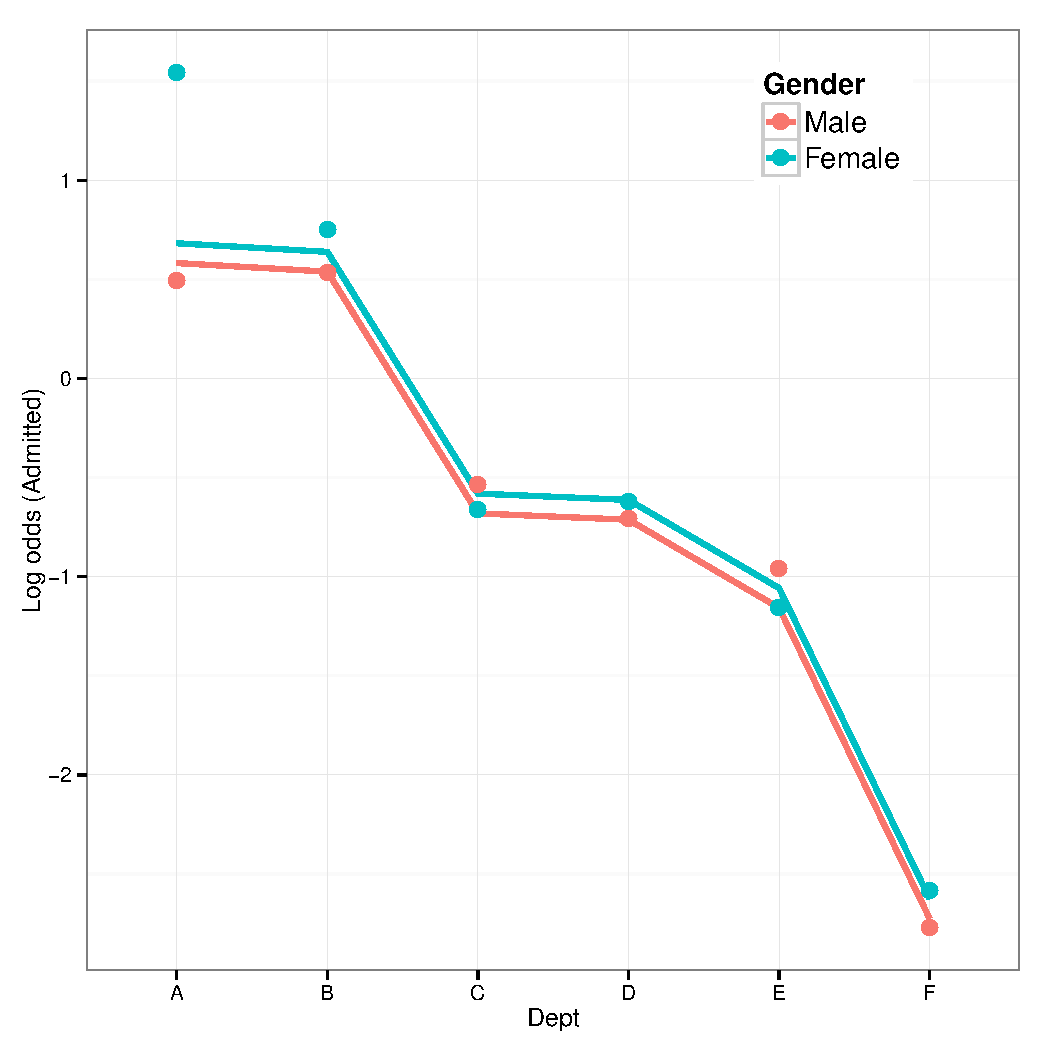
\includegraphics[width=0.49\textwidth]{ch08/fig/berk-logit2}
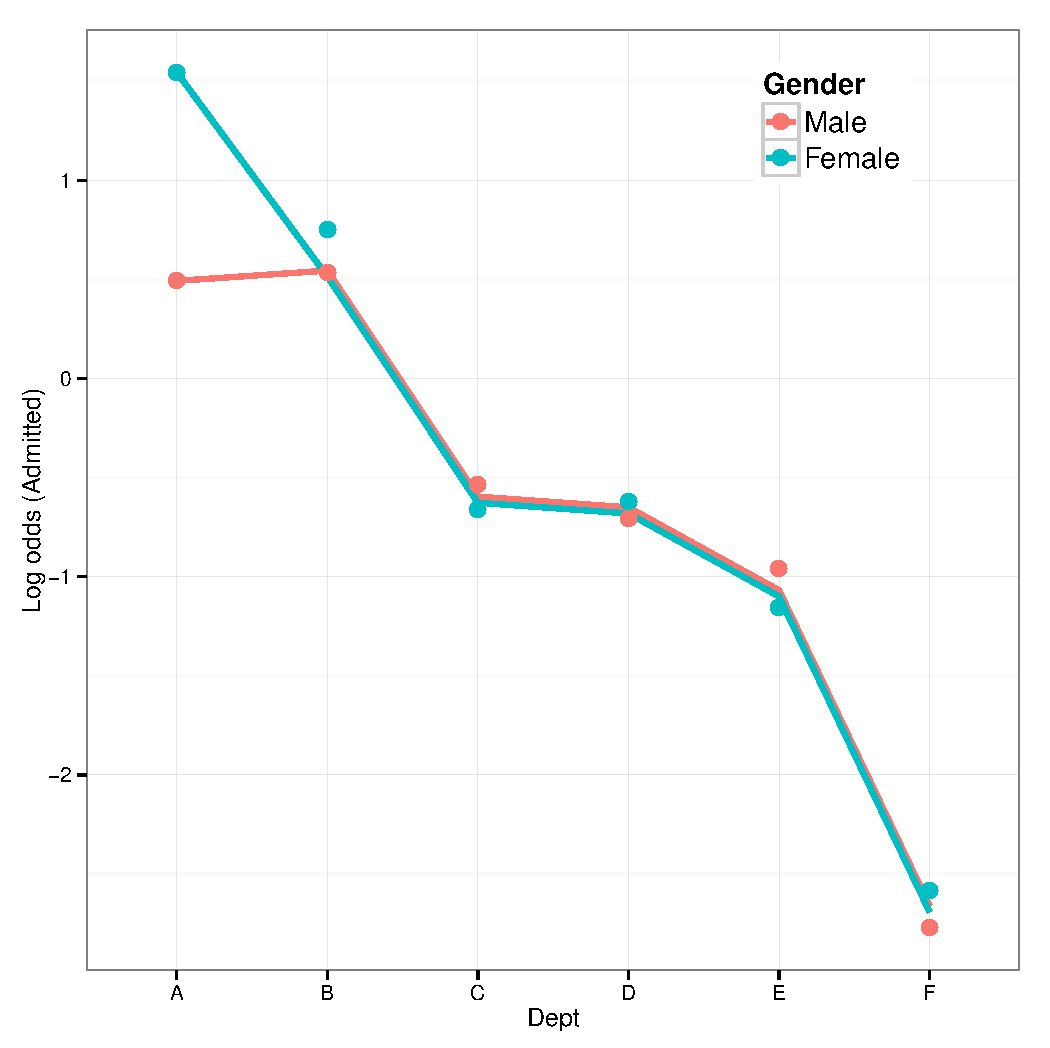
\includegraphics[width=0.49\textwidth]{ch08/fig/berk-logit3}
\caption{Observed (points) and fitted (lines) log odds of admissions in the logit models for
the \data{UCBAdmissions} data. Left: the logit model \eqref{eq:berk3} corresponding to the
\loglin model [AD] [AG] [DG]. Right: the logit model \eqref{eq:berk4}, allowing only a 1 df
term for Department A.}
\label{fig:berk-logit}
\end{figure}

The effects seen in our earlier analyses (Examples~\ref{ex:berkeley4},
\ref{ex:berkeley4b} and \ref{ex:berkeley6})
may all be observed in these plots.
In the left panel of \figref{fig:berk-logit},
corresponding to the \loglin model $\LLM{AD, AG, DG}$,
the effect of gender,  $\beta _j^{\mbox{\scriptsize Gender}}$,
in the equivalent logit model
is shown by the constant separation
between the two curves.
From the plot we see that this effect is very small (and nonsignificant).
In the right panel, corresponding to the logit model \eqref{eq:berk4},
there is no effect of gender on admission, except in department A, where the
extra parameter allows perfect fit.


\end{Example}

\section{Zero frequencies}\label{sec:loglin-zeros}

Cells with frequencies of zero create problems for \loglin and logit
models.  For \loglin models, most of the derivations of
expected
frequencies by maximum likelihood
and other quantities that depend on these (e.g., \GSQ tests)
assume that all $n_{ijk\cdots} > 0$.
In analogous
logit models, the observed log odds (e.g., for a three-way table),
$\log ( n_{ij1} / n_{ij2} )$, will be undefined if either frequency is
zero.

Zero frequencies may occur in \ctabs for two different reasons:
\begin{itemize}
\item \term{structural zeros} (also called \emph{fixed zeros}) will occur when it is impossible to observe
values for some combinations of the variables.
For these cases we should have $\widehat{m}_i$ = 0 wherever $n_i=0$.
For example, suppose we have three different methods of contacting
people at risk for some obscure genetically inherited disease:
newspaper advertisement, telephone campaign, and radio appeal.
If each person contacted in any way is classified dichotomously
by the three methods of contact, there can never be a non-zero
frequency in the `No-No-No' cell.%
\footnote{Yet, if we fit an unsaturated model, expected frequencies
may be estimated for all cells, and provide a means to estimate
the total number at risk in the population.
See \citet[Section 5.4]{Lindsey:95}.}
Similarly, in a tabulation of seniors by
gender and health concerns, there
can never be males citing menopause or females citing prostate cancer.
Square tables, such as wins and losses for sporting teams often have
structural zeros in the main diagonal.

\item \term{sampling zeros} (also called \emph{random zeros})
occur when the total size of the sample is not large enough in relation to the probabilities in each of the cells to assure that someone will be observed
in every cell. Here, it is permissible to have $\widehat{m}_i$ > 0 when $n_i=0$.
This problem increases with the number of table variables.
For example, in a European survey of religious affiliation, gender and occupation,
we may not happen to observe any female Muslim vineyard-workers in France, although such individuals surely exist in the population.
Even when zero frequencies do not occur, tables with many cells relative to
the total frequency tend to produce small expected frequencies in at
least some cells, which tends to make  the \GSQ statistics for model fit
and \LR statistics for individual terms unreliable.
\end{itemize}

Following \citet{Birch:1963}, \citet{Haberman:74} and many others \citep[e.g.,][]{Bishop-etal:75}
identified conditions under which the maximum likelihood estimate for
a given \loglin model does not exist, meaning that the algorithms used in
\func{loglin} and \func{glm} do not converge to a solution.
The problem depends on the number and locations of the zero cells, but not on the
size of the frequencies in the remaining cells.
\citet{FienbergAlessandro:2007} give a historical overview of the problem
and current approaches and \citet[\S 10.6]{Agresti:2013} gives a compact
summary.

In \R, the mechanism to handle structural zeros in the IPF approach of
\func{loglin} and \func{loglm} is to supply the argument \code{start},
giving a table conforming to the data, containing values of 0 in
the locations of the zero cells, and non-zero elsewhere.%
\footnote{
If structural zeros are present, the calculation of degrees of freedom may not be correct. \func{loglm} deducts one degree of freedom for each structural zero, but cannot make allowance for
patterns of zeros based on the fitted margins that lead to
gains in degrees of freedom due to smaller dimension in the parameter space.
\func{loglin} makes no such correction.
}
In the \func{glm} approach, the argument \code{subset=Freq > 0} can be
used to remove the cells with zero frequencies from the data,
or else, zero frequencies can be set to \code{NA}.
This usually  provides the correct degrees of freedom, however some estimated
coefficients may be infinite.

For a complete table, the residual degrees of freedom are determined as
\begin{equation*}
df = \mbox{\# of cells} - \mbox{\# of fitted parameters}
\end{equation*}
For tables with structural zeros, an analogous general formula is
\begin{equation}\label{eq:dfzeros}
df = (\mbox{\# cells} - \mbox{\# of parameters})
   - (\mbox{\# zero cells} - \mbox{\# of NA parameters})
\end{equation}
where NA parameters refers to parameters that cannot be estimated
due to zero marginal totals in the model formula.


In contrast, sampling zeros are often handled by some modification of the
data frequencies to ensure all non-zero cells.
Some suggestions are:
\begin{itemize*}
\item Add a small positive quantity (0.5 is often recommended) to \emph{every}
cell in the \ctab \citep{Goodman:70}, as is often done in calculating
empirical log odds (\exref{ex:toxaemia}); this simple approach over-smooths the
data for unsaturated models, and should be deprecated, although widely
used in practice.

\item Replace sampling zeros by some small number, typically
$10^{-10}$ or smaller \citep{Agresti:90}.
\item Add a small quantity, like 0.1, to \emph{all} zero cells, sampling or structural
\citep{EversNamboodiri:77}.
\end{itemize*}
In complex, sparse tables, a sensitivity analysis, comparing different approaches can help determine if the substantive conclusions vary with the approach to zero cells.

\begin{Example}[health]{Health concerns of teenagers}
\citet[Table 8-3]{Fienberg:80} presented a classic example of structural
zeros in the analysis of the $4 \times 2 \times 2$
table shown in \tabref{tab:health}.  The data come from a survey of
health concerns among teenagers, originally from \citet{Brunswick:1971}.
Among the health concerns, the two zero entries for menstrual problems
among males are clearly structural zeros and there therefore one
structural zero in the concern by gender marginal table.
As usual, we abbreviate the table variables concern, age, gender
by their initial letters, C, A, G below.

%\documentclass{standalone}
%\usepackage{float}
%\begin{document}
% latex table generated in R 3.0.1 by xtable 1.7-3 package
% Sun May 25 09:42:32 2014
\begin{table}[htb]
\centering
\caption{Results from a survey of teenagers, regarding their health concerns. Two cells with structural zeros are highlighted.  \emph{Source:}
  \citet[Table 8-3]{Fienberg:80} }
\label{tab:health}
\begin{tabular}{l|rrrrr}
%  \hline
% & 1 & 2 & 3 & 4 & 5 & 6 \\
  \hline
 Health     &  Gender:  &  \multicolumn{2}{c}{Male}  & \multicolumn{2}{c}{Female}  \\
 Concerns   &  Age:     &  12-15  &  16-17  &  12-15  &  16-17  \\
  \hline
  sex, reproduction  &          &       4 &       2 &       9 &       7 \\
  menstrual problems &          & \textbf{0} & \textbf{0} &       4 &       8 \\
  how healthy I am   &          &      42 &       7 &      19 &      10 \\
  nothing            &          &      57 &      20 &      71 &      21 \\
   \hline
\end{tabular}
\end{table}
%\end{document}


The \data{Health} data is created as a frequency data frame as follows.
\begin{knitrout}
\definecolor{shadecolor}{rgb}{1, 0.961, 0.933}\color{fgcolor}\begin{kframe}
\begin{alltt}
\hlstd{Health} \hlkwb{<-} \hlkwd{expand.grid}\hlstd{(}\hlkwc{concerns} \hlstd{=} \hlkwd{c}\hlstd{(}\hlstr{"sex"}\hlstd{,} \hlstr{"menstrual"}\hlstd{,}
                                   \hlstr{"healthy"}\hlstd{,} \hlstr{"nothing"}\hlstd{),}
                      \hlkwc{age}      \hlstd{=} \hlkwd{c}\hlstd{(}\hlstr{"12-15"}\hlstd{,} \hlstr{"16-17"}\hlstd{),}
                      \hlkwc{gender}   \hlstd{=} \hlkwd{c}\hlstd{(}\hlstr{"M"}\hlstd{,} \hlstr{"F"}\hlstd{))}
\hlstd{Health}\hlopt{$}\hlstd{Freq} \hlkwb{<-} \hlkwd{c}\hlstd{(}\hlnum{4}\hlstd{,} \hlnum{0}\hlstd{,} \hlnum{42}\hlstd{,} \hlnum{57}\hlstd{,} \hlnum{2}\hlstd{,} \hlnum{0}\hlstd{,} \hlnum{7}\hlstd{,} \hlnum{20}\hlstd{,}
                 \hlnum{9}\hlstd{,} \hlnum{4}\hlstd{,} \hlnum{19}\hlstd{,} \hlnum{71}\hlstd{,} \hlnum{7}\hlstd{,} \hlnum{8}\hlstd{,} \hlnum{10}\hlstd{,} \hlnum{21}\hlstd{)}
\end{alltt}
\end{kframe}
\end{knitrout}
In this form, we first use \func{glm} to fit two small models,
neither of which involves the $\{C G\}$ margin.
Model \code{health.glm0} is the model of mutual independence, $\LLM{C,A,G}$.
Model \code{health.glm1} is the model of joint independence, $\LLM{C,AG}$,
allowing an association between age and gender, but neither with concern.
As noted above, the argument \code{subset=(Freq>0)} is used to
eliminate the structural zero cells.

\begin{knitrout}
\definecolor{shadecolor}{rgb}{1, 0.961, 0.933}\color{fgcolor}\begin{kframe}
\begin{alltt}
\hlstd{health.glm0} \hlkwb{<-}\hlkwd{glm}\hlstd{(Freq} \hlopt{~}  \hlstd{concerns} \hlopt{+} \hlstd{age} \hlopt{+} \hlstd{gender,} \hlkwc{data}\hlstd{=Health,}
                  \hlkwc{subset}\hlstd{=(Freq}\hlopt{>}\hlnum{0}\hlstd{),} \hlkwc{family}\hlstd{=poisson)}
\hlstd{health.glm1} \hlkwb{<-}\hlkwd{glm}\hlstd{(Freq} \hlopt{~}  \hlstd{concerns} \hlopt{+} \hlstd{age} \hlopt{*} \hlstd{gender,} \hlkwc{data}\hlstd{=Health,}
                  \hlkwc{subset}\hlstd{=(Freq}\hlopt{>}\hlnum{0}\hlstd{),} \hlkwc{family}\hlstd{=poisson)}
\end{alltt}
\end{kframe}
\end{knitrout}
Neither of these fits the data well.  To conserve space, we show only the
results of the \GSQ tests for model fit.
\begin{knitrout}
\definecolor{shadecolor}{rgb}{1, 0.961, 0.933}\color{fgcolor}\begin{kframe}
\begin{alltt}
\hlstd{vcdExtra::}\hlkwd{Summarise}\hlstd{(health.glm0, health.glm1)}
\end{alltt}
\begin{verbatim}
## Likelihood summary table:
##               AIC BIC LR Chisq Df Pr(>Chisq)    
## health.glm0 100.7 105     27.7  8    0.00053 ***
## health.glm1  99.9 104     24.9  7    0.00080 ***
## ---
## Signif. codes:  0 '***' 0.001 '**' 0.01 '*' 0.05 '.' 0.1 ' ' 1
\end{verbatim}
\end{kframe}
\end{knitrout}
To see why, \figref{fig:health-mosaic} shows the mosaic display for model
\code{health.glm1}, $\LLM{C, AG}$.  Note that \func{mosaic}
takes care to make cells of zero frequency more visible by
marking them with a small ``o'', as these have an area of zero.

\begin{knitrout}
\definecolor{shadecolor}{rgb}{1, 0.961, 0.933}\color{fgcolor}\begin{kframe}
\begin{alltt}
\hlkwd{mosaic}\hlstd{(health.glm1,} \hlopt{~}\hlstd{concerns}\hlopt{+}\hlstd{age}\hlopt{+}\hlstd{gender,} \hlkwc{residuals_type}\hlstd{=}\hlstr{"rstandard"}\hlstd{)}
\end{alltt}
\end{kframe}\begin{figure}[!htbp]


\centerline{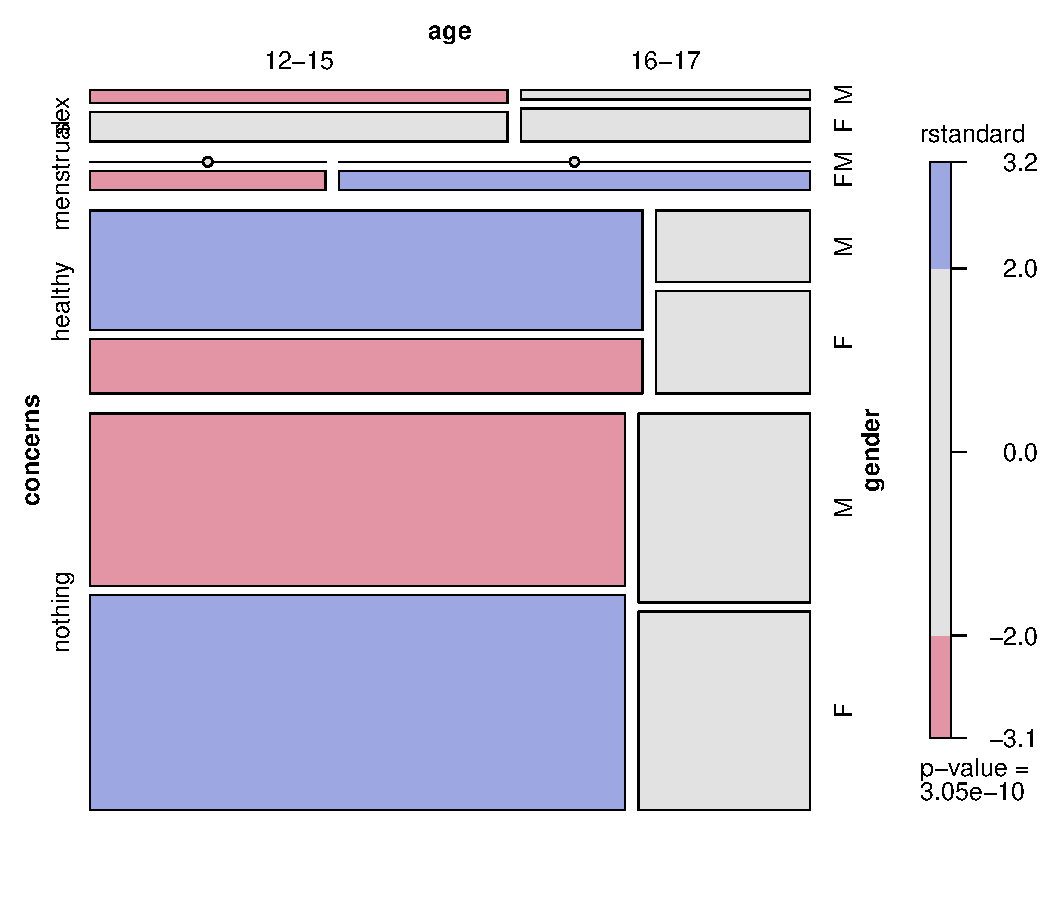
\includegraphics[width=.6\textwidth]{ch08/fig/health-mosaic-1} }

\caption[Mosaic display for the Health data, model health.glm1]{Mosaic display for the Health data, model \code{health.glm1}\label{fig:health-mosaic}}
\end{figure}


\end{knitrout}
This suggests that there are important associations at least between concern and gender
($[CG]$) and between concern and age ($[CA]$).
These are incorporated into the next model:
\begin{knitrout}
\definecolor{shadecolor}{rgb}{1, 0.961, 0.933}\color{fgcolor}\begin{kframe}
\begin{alltt}
\hlstd{health.glm2} \hlkwb{<-}\hlkwd{glm}\hlstd{(Freq} \hlopt{~}  \hlstd{concerns}\hlopt{*}\hlstd{gender} \hlopt{+} \hlstd{concerns}\hlopt{*}\hlstd{age,} \hlkwc{data}\hlstd{=Health,}
                  \hlkwc{subset}\hlstd{=(Freq}\hlopt{>}\hlnum{0}\hlstd{),} \hlkwc{family}\hlstd{=poisson)}
\hlstd{vcdExtra::}\hlkwd{Summarise}\hlstd{(health.glm2)}
\end{alltt}
\begin{verbatim}
## Likelihood summary table:
##              AIC  BIC LR Chisq Df Pr(>Chisq)
## health.glm2 87.7 94.7     4.66  3        0.2
\end{verbatim}
\end{kframe}
\end{knitrout}
The degrees of freedom are correct here.  \eqref{eq:dfzeros},
with 2 zero cells and 1 NA parameter due to the zero in the $\{CG\}$ margin
gives $df = (16-12) - (2-1) = 3$.  The loss of one estimable parameter
can be seen in the output from \code{summary}.
\begin{knitrout}\footnotesize
\definecolor{shadecolor}{rgb}{1, 0.961, 0.933}\color{fgcolor}\begin{kframe}
\begin{alltt}
\hlkwd{summary}\hlstd{(health.glm2)}
\end{alltt}
\begin{verbatim}
## 
## Call:
## glm(formula = Freq ~ concerns * gender + concerns * age, family = poisson, 
##     data = Health, subset = (Freq > 0))
## 
## Deviance Residuals: 
##      1       3       4       5       7       8       9      10      11      12  
##  0.236   0.585  -0.173  -0.300  -1.202   0.302  -0.149   0.000  -0.795   0.158  
##     13      14      15      16  
##  0.176   0.000   1.348  -0.282  
## 
## Coefficients: (1 not defined because of singularities)
##                            Estimate Std. Error z value Pr(>|z|)    
## (Intercept)                   1.266      0.445    2.84   0.0045 ** 
## concernsmenstrual            -0.860      0.586   -1.47   0.1425    
## concernshealthy               2.380      0.471    5.05  4.4e-07 ***
## concernsnothing               2.800      0.462    6.07  1.3e-09 ***
## genderF                       0.981      0.479    2.05   0.0405 *  
## age16-17                     -0.368      0.434   -0.85   0.3964    
## concernsmenstrual:genderF        NA         NA      NA       NA    
## concernshealthy:genderF      -1.505      0.533   -2.82   0.0047 ** 
## concernsnothing:genderF      -0.803      0.503   -1.60   0.1105    
## concernsmenstrual:age16-17    1.061      0.750    1.41   0.1574    
## concernshealthy:age16-17     -0.910      0.513   -1.77   0.0761 .  
## concernsnothing:age16-17     -0.771      0.469   -1.64   0.1005    
## ---
## Signif. codes:  0 '***' 0.001 '**' 0.01 '*' 0.05 '.' 0.1 ' ' 1
## 
## (Dispersion parameter for poisson family taken to be 1)
## 
##     Null deviance: 252.4670  on 13  degrees of freedom
## Residual deviance:   4.6611  on  3  degrees of freedom
## AIC: 87.66
## 
## Number of Fisher Scoring iterations: 4
\end{verbatim}
\end{kframe}
\end{knitrout}

In contrast, \func{loglm} reports the degrees of freedom incorrectly for
models containing zeros in any fitted margin.
For use with \func{loglm},  we convert it to a $4 \times 2 \times$ table.
\begin{knitrout}
\definecolor{shadecolor}{rgb}{1, 0.961, 0.933}\color{fgcolor}\begin{kframe}
\begin{alltt}
\hlstd{health.tab} \hlkwb{<-} \hlkwd{xtabs}\hlstd{(Freq} \hlopt{~} \hlstd{concerns} \hlopt{+} \hlstd{age} \hlopt{+} \hlstd{gender,} \hlkwc{data} \hlstd{= Health)}
\end{alltt}
\end{kframe}
\end{knitrout}
The same three models are fitted with \func{loglm} as shown below.
The locations of the positive frequencies are marked in the
array \code{nonzeros} and supplied as the value of the
\code{start} argument. 
%\TODO{Check whether this will work with Summarise()}
\begin{knitrout}
\definecolor{shadecolor}{rgb}{1, 0.961, 0.933}\color{fgcolor}\begin{kframe}
\begin{alltt}
\hlstd{nonzeros} \hlkwb{<-} \hlkwd{ifelse}\hlstd{(health.tab}\hlopt{>}\hlnum{0}\hlstd{,} \hlnum{1}\hlstd{,} \hlnum{0}\hlstd{)}
\hlstd{health.loglm0} \hlkwb{<-} \hlkwd{loglm}\hlstd{(}\hlopt{~} \hlstd{concerns} \hlopt{+} \hlstd{age} \hlopt{+} \hlstd{gender,}
              \hlkwc{data} \hlstd{= health.tab,} \hlkwc{start} \hlstd{= nonzeros)}
\hlstd{health.loglm1} \hlkwb{<-} \hlkwd{loglm}\hlstd{(}\hlopt{~} \hlstd{concerns} \hlopt{+} \hlstd{age} \hlopt{*} \hlstd{gender,}
              \hlkwc{data} \hlstd{= health.tab,} \hlkwc{start} \hlstd{= nonzeros)}
\hlcom{# df is wrong}
\hlstd{health.loglm2} \hlkwb{<-} \hlkwd{loglm}\hlstd{(}\hlopt{~} \hlstd{concerns}\hlopt{*}\hlstd{gender} \hlopt{+} \hlstd{concerns}\hlopt{*}\hlstd{age,}
              \hlkwc{data} \hlstd{= health.tab,} \hlkwc{start} \hlstd{= nonzeros)}
\hlkwd{Summarise}\hlstd{(health.loglm0, health.loglm1, health.loglm2)}
\end{alltt}
\begin{verbatim}
## Likelihood summary table:
##                 AIC BIC LR Chisq Df Pr(>Chisq)    
## health.loglm0 104.7 111    27.74  8    0.00053 ***
## health.loglm1 103.9 111    24.89  7    0.00080 ***
## health.loglm2  93.7 104     4.66  2    0.09724 .  
## ---
## Signif. codes:  0 '***' 0.001 '**' 0.01 '*' 0.05 '.' 0.1 ' ' 1
\end{verbatim}
\end{kframe}
\end{knitrout}
% \TODO{Test bug fix with Summarise()}
% <<health-loglm2-test>>=
% Summarise(health.loglm0, health.loglm1, health.loglm2)
% @

The results agree with those of \func{glm}, except for the degrees of freedom
for the last model.

\end{Example}



\section{Models for ordinal variables}\label{sec:loglin-ordinal}

%\section{Models for ordinal variables}\label{sec:loglin-ordinal}
Standard \loglin models treat all classification variables as
nominal, unordered factors. In these models,
all statistical tests are identical
and parameter estimates are equivalent
if the categories of any of the table variable are reordered.
Yet we have seen that the ordering of categories often provides
important information about the nature of associations
and we showed (\secref{sec:ordinaltests}) that non-parametric
tests which take into account the ordered nature of a factor
are more powerful.

Correspondence analysis plots (\chref{ch:corresp}) make it easy
to see the relationships between ordinal variables, because
the method assigns quantitative scores to the table variables
which maximally account for their association.
As we saw for the hair-eye color data (\figref{fig:ca-haireye-plot})
and the mental impairment data (\figref{fig:ca-mental-plot}),
an association can be interpreted in terms of ordered categories
when the points for two factors are ordered similarly, usually
along the first CA dimension.

Similarly, in a mosaic display, an ordered associative effect is seen when
the residuals have an opposite-corner pattern of positive and negative
signs and magnitudes (e.g., for the hair-eye color data,
\figref{fig:haireye-mos9}%
%or the Titanic data, \figref{fig:mostitanic1}
).
In these cases \loglin and logit models which use the ordered nature of the factors
offer several advantages.

\begin{itemize}
\item Because they are more focused, tests which use the ordinal
structure of the table variables are more powerful when the association
varies systematically with the ordered values of a factor.

\item Because they consume fewer degrees of freedom,
we can fit unsaturated models where the corresponding model for
nominal factors would be saturated.
In a two-way table, for example, a variety of models for ordinal
factors may be proposed which are intermediate between the independence
model and the saturated model.

\item Parameter estimates from these models are fewer in number, are
easier to interpret, and quantify the nature of effects better
than corresponding quantities in models for nominal factors.
Estimating fewer parameters typically gives smaller standard errors.
%as we saw in \exref{ex:reagan}.
\end{itemize}
These advantages are analogous to the use of tests for trends or
polynomial contrasts in ANOVA models.
More importantly, in some research areas in the social sciences
(where categorical data is commonplace), models for
ordinal variables have proved crucial in theory construction
and debates, giving more precise tests of hypotheses than
available from less focused or descriptive methods
\citep{Agresti:84}.

\subsection{Loglinear models for ordinal variables}\label{sec:loglin-ordlog}
For a two-way table, when either the row variable or the column variable,
or both, are ordinal, one simplification comes from assigning ordered
scores, $\vec{a}=\{a_i\}, a_1 \le a_2 \le \cdots a_I$, and/or
$\vec{b}=\{b_j\}, b_1 \le b_2 \le \cdots b_J$
to the categories
so that the ordinal relations are necessarily included in the model.
Typically, equally spaced scores are used, for example, integer
scores, $\{a_i\}=i$, or the zero-sum equivalent, $\{a_i\}=i-(I+1)/2$
(e.g., $\{a_i\}= \{-1, 0, 1\}$ for $I=3$).

Using such scores gives simple interpretations of the
association parameters in terms of \emph{local odds ratios}
for adjacent $2 \times 2$ subtables,
\begin{equation}\label{eq:loddsratios}
 \theta_{ij} =
 \frac{ m_{ij} \: m_{i+1, j+1} } { m_{i,j+1} \: m_{i+1, j} }
 \comma
\end{equation}
which is the odds ratio for pairs of adjacent rows and adjacent columns.


When both variables are assigned scores, this gives the \term{linear-by-linear model}
($L \times L$)
\begin{equation}\label{eq:linlin}
\log ( m_{ij} ) = \mu  +  \lambda_i^A
+  \lambda_j^B  +  \gamma \: a_i b_j \period
\end{equation}
Because the scores $\vec{a}$ and $\vec{b}$
are fixed, this model has only one extra parameter, $\gamma$, compared to the
independence model, which is the special case, $\gamma=0$.  In contrast,
the saturated model, allowing general association $\lambda_{ij}^{AB}$
uses $(I-1)(J-1)$ additional parameters.

The terms  $\gamma a_i b_j $ in \eqref{eq:linlin}
describe a pattern of association
where deviations from independence increase linearly with $a_i$
and $b_j$ in opposite directions towards the opposite corners of
the table, as we have often observed in mosaic displays.

In the linear-by-linear association model, the local log odds ratios
are
\begin{equation*}
\log (\theta_{ij}) =
 \gamma (a_{i+1} - a_i) (b_{j+1} - b_j)
 \comma
\end{equation*}
which reduces to
\begin{equation*}
\log (\theta_{ij}) =
 \gamma
\end{equation*}
for integer-spaced scores, so $\gamma$ is the common local log odds ratio.
As a result, the linear-by-linear model is sometimes called the
\term{uniform association model} \citep{Goodman:79}.
\ix{uniform association model}
\ix{linear-by-linear model}
\ix{log odds ratio!local}

Generalizations of the linear-by-linear model result when only one
variable is assigned scores.
In the \term{row effects model} (R),
the row variable, $A$, is treated as nominal, while
the column variable, $B$, is assigned ordered scores $\{b_j\}$.
The \loglin model is then
\begin{equation}\label{eq:roweff}
 \log ( m_{ij} ) = \mu  +  \lambda_i^A
  +  \lambda_j^B  +  \alpha_i b_j
 \comma
\end{equation}
where the $\alpha_i$ parameters are the \emph{row effects}.
An additional constraint,
$\sum_i \alpha_i =0$ or $\alpha_1 =0$
is imposed, so that model \eqref{eq:roweff}
has only $(I-1)$ more parameters than the independence model.
The linear-by-linear model is the special case where the row effects
are equally spaced, and the independence model is the special case
where all $\alpha_i = 0$.

The row-effects model \eqref{eq:roweff} also has a simple odds ratio interpretation.
The local log odds ratio for adjacent pairs of rows and columns is
\begin{equation*}
\log (\theta_{ij}) =
  \alpha_{i+1} - \alpha_i
  \comma
\end{equation*}
which is constant for all pairs of adjacent columns.  Plots of the
local log odds ratio against $i$ would appear as a set of parallel
curves.

In the analogous \term{column effects model} (C), $(J-1)$ linearly independent
column effect
parameters $\beta_j$ are estimated for the column variable, while fixed
scores $\{a_i\}$ are assigned to the row variable. It is also possible to
fit a \term{row plus column effects model} (R+C), that assigns specified
scores to both the rows and column variables.

Nesting relationships among these models and others described in
\secref{sec:RCmodels}
are shown in \figref{fig:assoc-models}.
Any set of models connected by a path can be directly compared with
\LR tests of the form $\GSQ (M_2 | M_1)$.

\begin{figure}
  \centering
  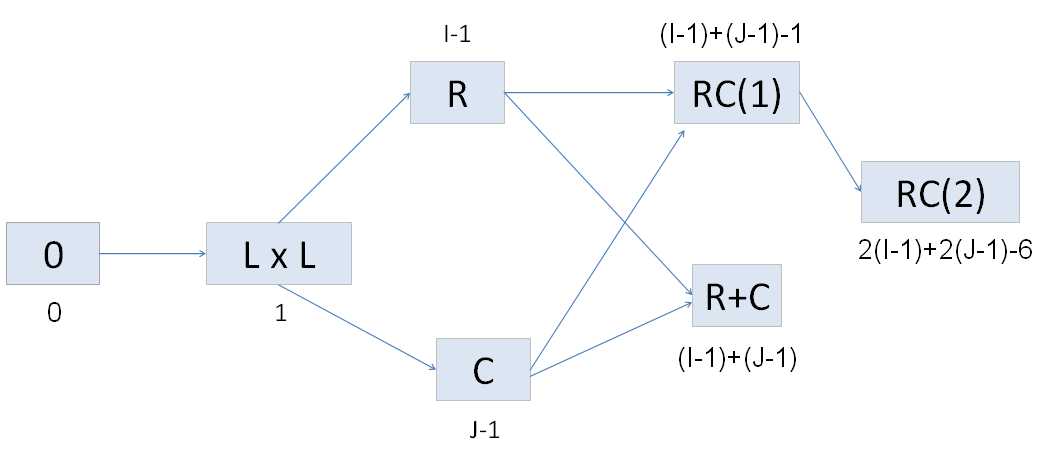
\includegraphics[width=\textwidth]{ch08/fig/assoc-models}
  \caption{Nesting relationships among some association models for an $I \times J$ table
  specifying the association parameters, $\lambda{ij}^{AB}$.
  Model \textbf{0} is the independence model.
  Formulas near the boxes give the number of identifiable association parameters.
  Arrows point from one nested model to another that is a more general version.}
  \label{fig:assoc-models}
\end{figure}

In \R, the $L \times L$, row effects and column effects models can
all be fit using \func{glm} simply by replacing the appropriate
table factor variable(s) with their \func{as.numeric}
equivalents.

\begin{Example}[mental4]{Mental impairment and parents' SES}
The \data{Mental} data on the mental health status of young
New York residents in relation to their parents'
socioeconomic status was
examined in \exref{ex:mental2} using CMH tests for ordinal
association and in \exref{ex:mental3} using \ca.
\figref{fig:ca-mental-plot} showed that nearly all of the association in the
table was accounted for by a single dimension along which both factors
were ordered, consistent with the view that mental health increased
in relation to parents' SES.

Because these models provide their interpretations in terms of local odds
ratios, \eqref{eq:loddsratios},
it is helpful to see these values for the observed data,
corresponding to the saturated model.  The values
$\log(\theta_{ij})$ are calculated by
\func{loddsratio} in \pkg{vcdExtra}, with the data in table form.
\begin{knitrout}
\definecolor{shadecolor}{rgb}{1, 0.961, 0.933}\color{fgcolor}\begin{kframe}
\begin{alltt}
\hlstd{(mental.tab} \hlkwb{<-} \hlkwd{xtabs}\hlstd{(Freq} \hlopt{~} \hlstd{mental}\hlopt{+}\hlstd{ses,} \hlkwc{data}\hlstd{=Mental))}
\end{alltt}
\begin{verbatim}
##           ses
## mental       1   2   3   4   5   6
##   Well      64  57  57  72  36  21
##   Mild      94  94 105 141  97  71
##   Moderate  58  54  65  77  54  54
##   Impaired  46  40  60  94  78  71
\end{verbatim}
\begin{alltt}
\hlkwd{loddsratio}\hlstd{(mental.tab)}
\end{alltt}
\begin{verbatim}
## log odds ratios for mental and ses 
## 
##                    ses
## mental                  1:2    2:3     3:4    4:5    5:6
##   Well:Mild          0.1158 0.1107  0.0612 0.3191  0.227
##   Mild:Moderate     -0.0715 0.0747 -0.1254 0.0192  0.312
##   Moderate:Impaired -0.0683 0.2201  0.2795 0.1682 -0.094
\end{verbatim}
\end{kframe}
\end{knitrout}

\begin{figure}[!htb]
\centering
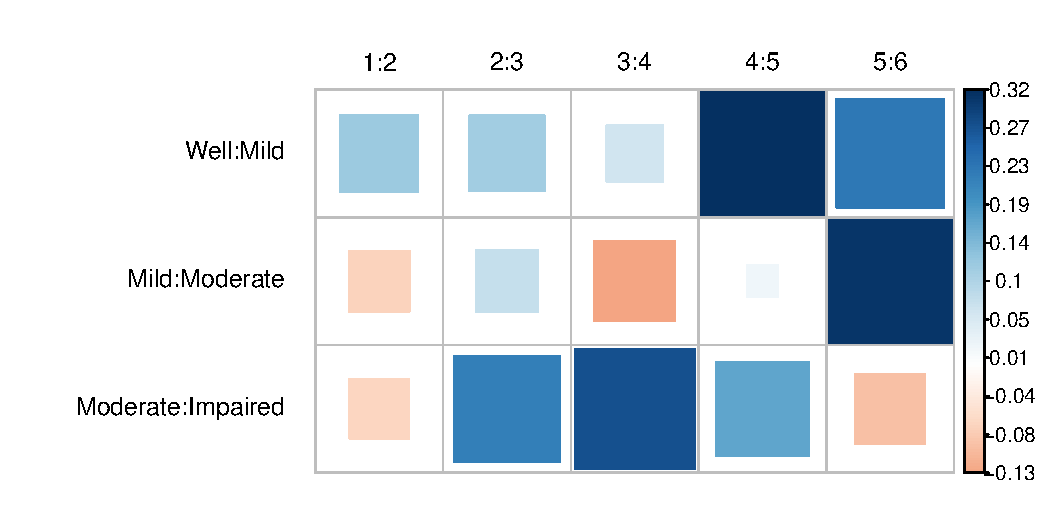
\includegraphics[width=.75\textwidth]{ch08/fig/mental-lorplot}
\caption{Shaded-square plot of the local odds ratios in the \data{Mental} data.}
\label{fig:mental-lorplot}
\end{figure}

A simple plot of these values, using area- and color-proportional shaded squares is shown in
\figref{fig:mental-lorplot}. This plot is drawn using the \Rpackage{corrplot}.
It is easy to see that most of the local odds ratios are mildly positive.
\begin{knitrout}
\definecolor{shadecolor}{rgb}{1, 0.961, 0.933}\color{fgcolor}\begin{kframe}
\begin{alltt}
\hlstd{M} \hlkwb{<-} \hlkwd{as.matrix}\hlstd{(}\hlkwd{loddsratio}\hlstd{(mental.tab))}
\hlkwd{library}\hlstd{(corrplot)}
\hlkwd{corrplot}\hlstd{(M,} \hlkwc{method}\hlstd{=}\hlstr{"square"}\hlstd{,} \hlkwc{is.corr}\hlstd{=}\hlnum{FALSE}\hlstd{,}
         \hlkwc{tl.col}\hlstd{=}\hlstr{"black"}\hlstd{,} \hlkwc{tl.srt}\hlstd{=}\hlnum{0}\hlstd{,} \hlkwc{tl.offset}\hlstd{=}\hlnum{1}\hlstd{)}
\end{alltt}
\end{kframe}
\end{knitrout}


For comparison with the $L \times L$ model fitted below, the mean
local log odds ratio is 0.103.
\begin{knitrout}
\definecolor{shadecolor}{rgb}{1, 0.961, 0.933}\color{fgcolor}\begin{kframe}
\begin{alltt}
\hlkwd{mean}\hlstd{(}\hlkwd{loddsratio}\hlstd{(mental.tab)}\hlopt{$}\hlstd{coefficients)}
\end{alltt}
\begin{verbatim}
## [1] 0.10323
\end{verbatim}
\end{kframe}
\end{knitrout}


As a baseline, we first fit the independence model
(testing $H_0: \log(\theta_{ij})=0$)
with \func{glm}.
As expected, this model fits quite badly,
with $\GSQ\ (15) = 47.418$.

\begin{knitrout}
\definecolor{shadecolor}{rgb}{1, 0.961, 0.933}\color{fgcolor}\begin{kframe}
\begin{alltt}
\hlstd{indep} \hlkwb{<-} \hlkwd{glm}\hlstd{(Freq} \hlopt{~} \hlstd{mental} \hlopt{+} \hlstd{ses,}
                \hlkwc{family} \hlstd{= poisson,} \hlkwc{data} \hlstd{= Mental)}
\hlstd{vcdExtra::}\hlkwd{Summarise}\hlstd{(indep)}
\end{alltt}
\begin{verbatim}
## Likelihood summary table:
##       AIC BIC LR Chisq Df Pr(>Chisq)    
## indep 210 220     47.4 15    3.2e-05 ***
## ---
## Signif. codes:  0 '***' 0.001 '**' 0.01 '*' 0.05 '.' 0.1 ' ' 1
\end{verbatim}
\end{kframe}
\end{knitrout}
The mosaic display of standardized residuals from this model is shown
in \figref{fig:mental-indep}.  The argument \code{labeling=labeling\_residuals}
is used to show the numerical values in the cells with absolute values greater
than \code{suppress=1}.
\begin{knitrout}
\definecolor{shadecolor}{rgb}{1, 0.961, 0.933}\color{fgcolor}\begin{kframe}
\begin{alltt}
\hlstd{long.labels} \hlkwb{<-} \hlkwd{list}\hlstd{(}\hlkwc{set_varnames} \hlstd{=} \hlkwd{c}\hlstd{(}\hlkwc{mental}\hlstd{=}\hlstr{"Mental Health Status"}\hlstd{,}
                                     \hlkwc{ses}\hlstd{=}\hlstr{"Parent SES"}\hlstd{))}
\hlkwd{mosaic}\hlstd{(indep,}
       \hlkwc{gp}\hlstd{=shading_Friendly,}
       \hlkwc{residuals_type}\hlstd{=}\hlstr{"rstandard"}\hlstd{,}
       \hlkwc{labeling_args} \hlstd{= long.labels,}
       \hlkwc{labeling}\hlstd{=labeling_residuals,} \hlkwc{suppress}\hlstd{=}\hlnum{1}\hlstd{,}
       \hlkwc{main}\hlstd{=}\hlstr{"Mental health data: Independence"}\hlstd{)}
\end{alltt}
\end{kframe}\begin{figure}[!htbp]


\centerline{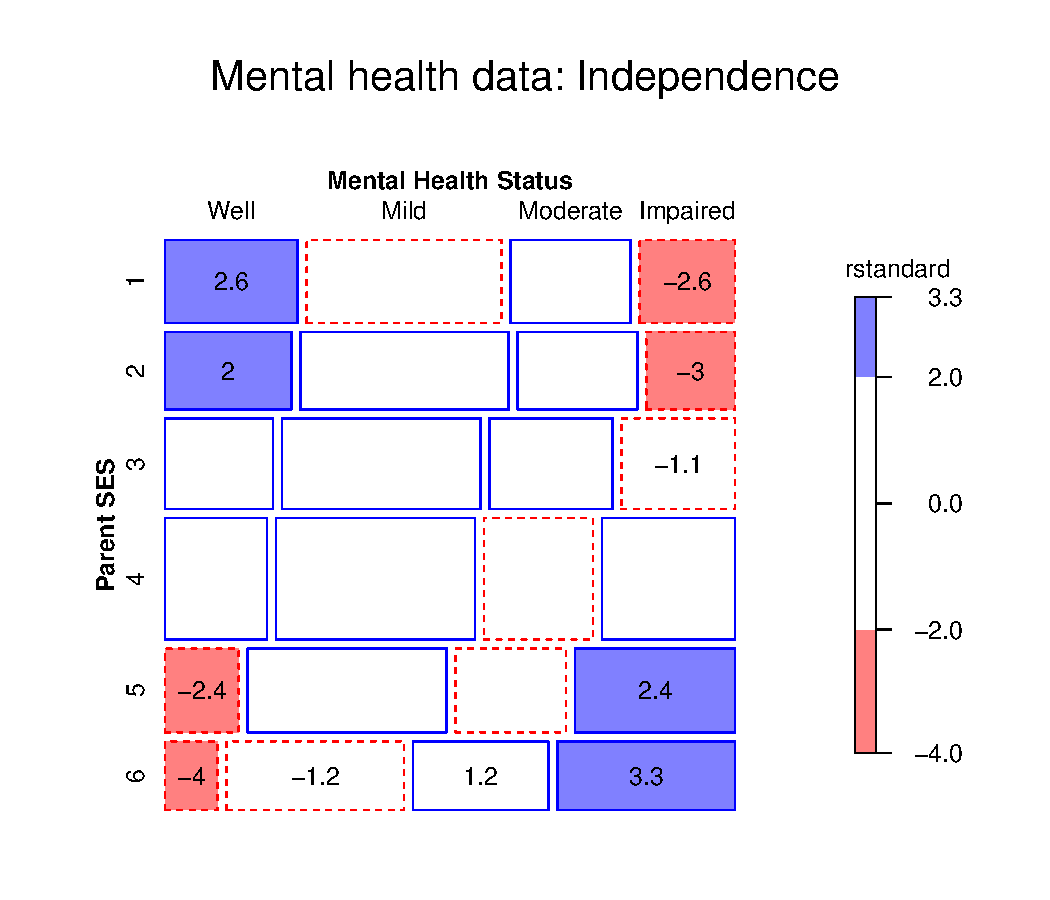
\includegraphics[width=.7\textwidth]{ch08/fig/mental-indep-1} }

\caption[Mosaic display of the independence model for the mental health data]{Mosaic display of the independence model for the mental health data.\label{fig:mental-indep}}
\end{figure}


\end{knitrout}
This figure shows the classic opposite-corner pattern of the signs and magnitudes of
the residuals that would
arise if the association between mental health and SES
was could be explained by the ordinal relation of these factors
using one of the $L \times L$, $R$ or $C$ models.

To fit such ordinal models, you can use \func{as.numeric} on a factor variable
to assign integer scores, or assign other values if integer spacing is not
appropriate.

\begin{knitrout}
\definecolor{shadecolor}{rgb}{1, 0.961, 0.933}\color{fgcolor}\begin{kframe}
\begin{alltt}
\hlstd{Cscore} \hlkwb{<-} \hlkwd{as.numeric}\hlstd{(Mental}\hlopt{$}\hlstd{ses)}
\hlstd{Rscore} \hlkwb{<-} \hlkwd{as.numeric}\hlstd{(Mental}\hlopt{$}\hlstd{mental)}
\end{alltt}
\end{kframe}
\end{knitrout}
Then, the $L \times L$, $R$ and $C$ models can be fit as follows, where
beyond the main effects of \code{mental} and \code{ses}, their association
is represented as the interaction of the numeric score(s) or factor(s),
as appropriate in each case.
\begin{knitrout}
\definecolor{shadecolor}{rgb}{1, 0.961, 0.933}\color{fgcolor}\begin{kframe}
\begin{alltt}
\hlstd{linlin} \hlkwb{<-} \hlkwd{glm}\hlstd{(Freq} \hlopt{~} \hlstd{mental} \hlopt{+} \hlstd{ses} \hlopt{+} \hlstd{Rscore}\hlopt{:}\hlstd{Cscore,}
              \hlkwc{family} \hlstd{= poisson,} \hlkwc{data} \hlstd{= Mental)}
\hlstd{roweff} \hlkwb{<-} \hlkwd{glm}\hlstd{(Freq} \hlopt{~} \hlstd{mental} \hlopt{+} \hlstd{ses} \hlopt{+} \hlstd{mental}\hlopt{:}\hlstd{Cscore,}
              \hlkwc{family} \hlstd{= poisson,} \hlkwc{data} \hlstd{= Mental)}
\hlstd{coleff} \hlkwb{<-} \hlkwd{glm}\hlstd{(Freq} \hlopt{~} \hlstd{mental} \hlopt{+} \hlstd{ses} \hlopt{+} \hlstd{Rscore}\hlopt{:}\hlstd{ses,}
              \hlkwc{family} \hlstd{= poisson,} \hlkwc{data} \hlstd{= Mental)}
\end{alltt}
\end{kframe}
\end{knitrout}

Goodness-of-fit tests for these models are shown below. They show that all of the
$L \times L$, $R$ and $C$ models are acceptable in terms of the \LR \GSQ.
The $L \times L$ model, with only one more parameter than the independence model
is judged the best by both AIC and BIC.
\begin{knitrout}
\definecolor{shadecolor}{rgb}{1, 0.961, 0.933}\color{fgcolor}\begin{kframe}
\begin{alltt}
\hlstd{vcdExtra::}\hlkwd{Summarise}\hlstd{(indep, linlin, roweff, coleff)}
\end{alltt}
\begin{verbatim}
## Likelihood summary table:
##          AIC   BIC LR Chisq Df Pr(>Chisq)    
## indep  209.6 220.2    47.42 15   3.16e-05 ***
## linlin 174.1 185.8     9.90 14      0.770    
## roweff 174.4 188.6     6.28 12      0.901    
## coleff 179.0 195.5     6.83 10      0.741    
## ---
## Signif. codes:  0 '***' 0.001 '**' 0.01 '*' 0.05 '.' 0.1 ' ' 1
\end{verbatim}
\end{kframe}
\end{knitrout}

In cases where such overall tests are unclear, you can carry out tests of
nested sets of models using \func{anova}, giving tests of $\Delta \GSQ$.

\begin{knitrout}
\definecolor{shadecolor}{rgb}{1, 0.961, 0.933}\color{fgcolor}\begin{kframe}
\begin{alltt}
\hlkwd{anova}\hlstd{(indep, linlin, roweff,} \hlkwc{test}\hlstd{=}\hlstr{"Chisq"}\hlstd{)}
\end{alltt}
\begin{verbatim}
## Analysis of Deviance Table
## 
## Model 1: Freq ~ mental + ses
## Model 2: Freq ~ mental + ses + Rscore:Cscore
## Model 3: Freq ~ mental + ses + mental:Cscore
##   Resid. Df Resid. Dev Df Deviance Pr(>Chi)    
## 1        15       47.4                         
## 2        14        9.9  1     37.5    9e-10 ***
## 3        12        6.3  2      3.6     0.16    
## ---
## Signif. codes:  0 '***' 0.001 '**' 0.01 '*' 0.05 '.' 0.1 ' ' 1
\end{verbatim}
\begin{alltt}
\hlkwd{anova}\hlstd{(indep, linlin, coleff,} \hlkwc{test}\hlstd{=}\hlstr{"Chisq"}\hlstd{)}
\end{alltt}
\begin{verbatim}
## Analysis of Deviance Table
## 
## Model 1: Freq ~ mental + ses
## Model 2: Freq ~ mental + ses + Rscore:Cscore
## Model 3: Freq ~ mental + ses + Rscore:ses
##   Resid. Df Resid. Dev Df Deviance Pr(>Chi)    
## 1        15       47.4                         
## 2        14        9.9  1     37.5    9e-10 ***
## 3        10        6.8  4      3.1     0.55    
## ---
## Signif. codes:  0 '***' 0.001 '**' 0.01 '*' 0.05 '.' 0.1 ' ' 1
\end{verbatim}
\end{kframe}
\end{knitrout}

Under the $L \times L$ model, the estimate of the coefficient of
\code{Rscore:Cscore} is $\hat{\gamma} = 0.0907$ (s.e.=0.015) with unit-spaced scores,
as shown below.
\begin{knitrout}
\definecolor{shadecolor}{rgb}{1, 0.961, 0.933}\color{fgcolor}\begin{kframe}
\begin{alltt}
\hlcom{# interpret linlin association parameter}
\hlkwd{coef}\hlstd{(linlin)[[}\hlstr{"Rscore:Cscore"}\hlstd{]]}
\end{alltt}
\begin{verbatim}
## [1] 0.090687
\end{verbatim}
\begin{alltt}
\hlkwd{exp}\hlstd{(}\hlkwd{coef}\hlstd{(linlin)[[}\hlstr{"Rscore:Cscore"}\hlstd{]])}
\end{alltt}
\begin{verbatim}
## [1] 1.0949
\end{verbatim}
\end{kframe}
\end{knitrout}
\noindent This corresponds to a local odds ratio, $\hat{\theta}_{ij} = \exp (0.0907) = 1.095$.
This single number describes the association succinctly:
each step down the socioeconomic scale increases the odds of being classified
one step poorer in mental health by 9.5\%.

\end{Example}

\subsection{Log-multiplicative (RC) models}\label{sec:RCmodels}

The association models described above
are all more parsimonious and easier to interpret
than the saturated model.  However, they depend on assigning fixed
and possibly arbitrary scores to the variable categories.
A generalization of the $L \times L$ model that treats \emph{both}
row and column scores as parameters is the \term{row-and-column effects model} (RC(1))
suggested by \citet{Goodman:79},
\begin{equation}\label{eq:RC1}
\log ( m_{ij} ) = \mu  +  \lambda_i^A
+  \lambda_j^B  +  \gamma \: \alpha_i \beta_j \comma
\end{equation}
where $\gamma$, $\vec{\alpha}$ and $\vec{\beta}$ comprise
additional parameters to be estimated beyond the independence model.%
\footnote{
In contrast to the R, C and R+C models, RC models do not
assume that the categories are appropriately ordered
because the category scores are estimated from the data.
}
This model has a close connection with correspondence analysis
\citep{Goodman:85}, where the estimated scores
$\vec{\alpha}$ and $\vec{\beta}$ are analogous to \ca scores
on a first dimension.%
\footnote{
However, when estimated by maximum likelihood, the RC(1) model allows
\LR tests of parameters
and model fit, AIC and BIC statistics, and methods for estimating
standard errors of the parameters.
Such model-based methods are not available for \ca.
}
$\gamma$, called the \emph{intrinsic association coefficient}
is analogous to the same parameter in the $L \times L$ model.

For identifiability and interpretation
it is necessary to impose some normalization constraints on the
$\vec{\alpha}$ and $\vec{\beta}$.
An \emph{unweighted, unit standardized} solution forces
$\sum_i \alpha_i = \sum_j \beta_j =0$ and
$\sum_i \alpha_i^2 = \sum_j \beta_j^2 =1$.
Alternatively, and more akin to \ca solutions, the \emph{marginally weighted} solution
uses the marginal probabilities $\pi_{i+}$ of the row variable and $\pi_{+j}$
of the columns as weights.
\begin{eqnarray}
\sum_i \alpha_i \pi_{i+} & = & \sum_j \beta_j \pi_{+j} = 0 \label{eq:RC-constraints} \\
\sum_i \alpha_i^2 \pi_{i+} & = & \sum_j \beta_j^2 \pi_{+j} = 1 \nonumber
\end{eqnarray}


\citet{Goodman:86} generalized this to multiple bilinear terms
of the form $\gamma_k \: \alpha_{ik} \beta_{jk}$, with $M$ terms (the RC(M) model)
and showed that
\emph{all} associations in the saturated model could be expressed exactly as
\begin{equation}\label{eq:RCm}
\lambda_{ij}^{AB} =
 \sum_{k=1}^M  \gamma_k \: \alpha_{ik} \beta_{jk} \quad\quad M=\min{(I-1,\,  J-1)}
 \period
\end{equation}
In practice, models with fewer terms usually suffice.
For example, an RC(2) model with two multiplicative terms is analogous to
a two-dimensional \ca solution.
In addition to the normalization constraints for the RC(1) model,
parameters in an RC(M) model must satisfy the additional constraints
that the  (possibly weighted) scores for distinct dimensions are
orthogonal (uncorrelated), similar to \ca solutions.



The RC model is \emph{not} a \loglin model
because it contains a multiplicative term in the parameters.
This model and a wide variety of
other nonlinear models for categorical data
can be fit using \func{gnm} in the \Rpackage{gnm}.
This provides the basic machinery for extending \func{glm} models
to nonlinear terms, quite generally.
The function \func{rc} in the
\Rpackage{logmult} uses \func{gnm} for fitting, and
offers greater convenience in normalizing the
category scores, calculating standard errors and plotting.

\begin{Example}[mental5]{Mental impairment and parents' SES}

The \Rpackage{gnm} provides a number of functions that can be used in model formulas
for nonlinear association terms.  Among these, \func{Mult} expresses a multiplicative
association in terms of two (or more) factors. The RC(1) model for factors \code{A, B}
uses \code{Mult(A,B)} for the association term in \eqref{eq:RC1}.
Multiple multiplicative RC terms, as in \eqref{eq:RCm} can be expressed
using \code{instances(Mult(A,B), m)}.

To illustrate, we fit the RC(1) and RC(2) models to the \data{Mental} data using
\func{gnm}.  In this table, both factors are ordered, but we don't want to use
the default polynomial contrasts, so we set their contrast attributes
to \code{treatment}.

\begin{knitrout}
\definecolor{shadecolor}{rgb}{1, 0.961, 0.933}\color{fgcolor}\begin{kframe}
\begin{alltt}
\hlkwd{library}\hlstd{(gnm)}
\hlstd{Mental}\hlopt{$}\hlstd{mental} \hlkwb{<-} \hlkwd{C}\hlstd{(Mental}\hlopt{$}\hlstd{mental, treatment)}
\hlstd{Mental}\hlopt{$}\hlstd{ses} \hlkwb{<-} \hlkwd{C}\hlstd{(Mental}\hlopt{$}\hlstd{ses, treatment)}
\hlstd{RC1} \hlkwb{<-} \hlkwd{gnm}\hlstd{(Freq} \hlopt{~} \hlstd{mental} \hlopt{+} \hlstd{ses} \hlopt{+} \hlkwd{Mult}\hlstd{(mental, ses),}
           \hlkwc{family} \hlstd{= poisson,} \hlkwc{data} \hlstd{= Mental,} \hlkwc{verbose}\hlstd{=}\hlnum{FALSE}\hlstd{)}
\hlstd{RC2} \hlkwb{<-} \hlkwd{gnm}\hlstd{(Freq} \hlopt{~} \hlstd{mental} \hlopt{+} \hlstd{ses} \hlopt{+} \hlkwd{instances}\hlstd{(}\hlkwd{Mult}\hlstd{(mental, ses),}\hlnum{2}\hlstd{),}
           \hlkwc{family} \hlstd{= poisson,} \hlkwc{data} \hlstd{= Mental,} \hlkwc{verbose}\hlstd{=}\hlnum{FALSE}\hlstd{)}
\end{alltt}
\end{kframe}
\end{knitrout}

For comparison with the \loglin association models fit in \exref{ex:mental4}
we show the \GSQ goodness of fit tests for all these models.
The ordinal \loglin models and the RC models all fit well, with the
$L \times L$ model preferred on the basis of parsimony by AIC and BIC.
\begin{knitrout}
\definecolor{shadecolor}{rgb}{1, 0.961, 0.933}\color{fgcolor}\begin{kframe}
\begin{alltt}
\hlstd{vcdExtra::}\hlkwd{Summarise}\hlstd{(indep, linlin, roweff, coleff, RC1, RC2)}
\end{alltt}
\begin{verbatim}
## Likelihood summary table:
##          AIC   BIC LR Chisq Df Pr(>Chisq)    
## indep  209.6 220.2    47.42 15   3.16e-05 ***
## linlin 174.1 185.8     9.90 14      0.770    
## roweff 174.4 188.6     6.28 12      0.901    
## coleff 179.0 195.5     6.83 10      0.741    
## RC1    179.7 198.6     3.57  8      0.894    
## RC2    186.7 211.4     0.52  3      0.914    
## ---
## Signif. codes:  0 '***' 0.001 '**' 0.01 '*' 0.05 '.' 0.1 ' ' 1
\end{verbatim}
\end{kframe}
\end{knitrout}
The substantive difference between the $L \times L$ model and the RC(1)
model is whether the categories of mental health status and SES can be
interpreted as equally spaced along some latent continua, versus the
alternative that category spacing is unequal.
We can test this directly using the \LR test, $\GSQ(L \times L \given RC(1))$
Similarly, model \code{RC1} is nested within model \code{RC2},
so $\GSQ(RC(1) \given RC(2))$ gives a direct test of the need for a second
dimension.
\begin{knitrout}
\definecolor{shadecolor}{rgb}{1, 0.961, 0.933}\color{fgcolor}\begin{kframe}
\begin{alltt}
\hlkwd{anova}\hlstd{(linlin, RC1, RC2,} \hlkwc{test}\hlstd{=}\hlstr{"Chisq"}\hlstd{)}
\end{alltt}
\begin{verbatim}
## Analysis of Deviance Table
## 
## Model 1: Freq ~ mental + ses + Rscore:Cscore
## Model 2: Freq ~ mental + ses + Mult(mental, ses)
## Model 3: Freq ~ mental + ses + Mult(mental, ses, inst = 1) + Mult(mental, 
##     ses, inst = 2)
##   Resid. Df Resid. Dev Df Deviance Pr(>Chi)
## 1        14       9.90                     
## 2         8       3.57  6     6.32     0.39
## 3         3       0.52  5     3.05     0.69
\end{verbatim}
\end{kframe}
\end{knitrout}
We see that estimated scores for the categories in the model \code{RC1}
do not provide a significantly better fit, and there is even less evidence
for a second dimension of category parameters in the \code{RC2} model.

Nevertheless, for cases where RC models \emph{do} provide some advantage, it
is useful to know how to visualize the estimated category parameters.
The key to this is the function \func{getContrasts}
which
computes contrasts or scaled contrasts for a set of (non-eliminated) parameters from a
\class{gnm} model,
together with standard errors for the estimated contrasts following the methods
of
\citet{Firth:2003,FirthMenezes:2004}. The details are explained in
\help{getContrasts} and in \code{vignette("gnmOverview")} that comes with
the \Rpackage{gnm}.

The coefficients in the marginally-weighted solution \eqref{eq:RC-constraints}
can be obtained as follows.
\begin{knitrout}
\definecolor{shadecolor}{rgb}{1, 0.961, 0.933}\color{fgcolor}\begin{kframe}
\begin{alltt}
\hlstd{rowProbs} \hlkwb{<-} \hlkwd{with}\hlstd{(Mental,} \hlkwd{tapply}\hlstd{(Freq, mental, sum)} \hlopt{/} \hlkwd{sum}\hlstd{(Freq))}
\hlstd{colProbs} \hlkwb{<-} \hlkwd{with}\hlstd{(Mental,} \hlkwd{tapply}\hlstd{(Freq, ses, sum)} \hlopt{/} \hlkwd{sum}\hlstd{(Freq))}
\hlstd{mu} \hlkwb{<-} \hlkwd{getContrasts}\hlstd{(RC1,} \hlkwd{pickCoef}\hlstd{(RC1,} \hlstr{"[.]mental"}\hlstd{),}
                   \hlkwc{ref} \hlstd{= rowProbs,} \hlkwc{scaleWeights} \hlstd{= rowProbs)}
\hlstd{nu} \hlkwb{<-} \hlkwd{getContrasts}\hlstd{(RC1,} \hlkwd{pickCoef}\hlstd{(RC1,} \hlstr{"[.]ses"}\hlstd{),}
                   \hlkwc{ref} \hlstd{= colProbs,} \hlkwc{scaleWeights} \hlstd{= colProbs)}
\end{alltt}
\end{kframe}
\end{knitrout}
In our notation, the coefficients $\vec{\alpha}$ and $\vec{\beta}$ can be
extracted as the \code{qvframe} component of the \class{qv} object
returned by \func{getContrasts}.
\begin{knitrout}
\definecolor{shadecolor}{rgb}{1, 0.961, 0.933}\color{fgcolor}\begin{kframe}
\begin{alltt}
\hlstd{(alpha} \hlkwb{<-} \hlstd{mu}\hlopt{$}\hlstd{qvframe)}
\end{alltt}
\begin{verbatim}
##                             Estimate Std. Error
## Mult(., ses).mentalWell      1.67378    0.19043
## Mult(., ses).mentalMild      0.14009    0.20018
## Mult(., ses).mentalModerate -0.13669    0.27948
## Mult(., ses).mentalImpaired -1.41055    0.17418
\end{verbatim}
\begin{alltt}
\hlstd{(beta}  \hlkwb{<-} \hlstd{nu}\hlopt{$}\hlstd{qvframe)}
\end{alltt}
\begin{verbatim}
##                       Estimate Std. Error
## Mult(mental, .).ses1  1.111361    0.29921
## Mult(mental, .).ses2  1.120459    0.31422
## Mult(mental, .).ses3  0.370752    0.31915
## Mult(mental, .).ses4 -0.027006    0.27328
## Mult(mental, .).ses5 -1.009480    0.31470
## Mult(mental, .).ses6 -1.816647    0.28095
\end{verbatim}
\end{kframe}
\end{knitrout}

For plotting this RC(1) solution for the scaled category scores
together with their estimated standard errors,
a \func{dotchart}, shown in \figref{fig:mental-RC1}
provides a reasonable visualization.

\begin{figure}[!htb]
\centering
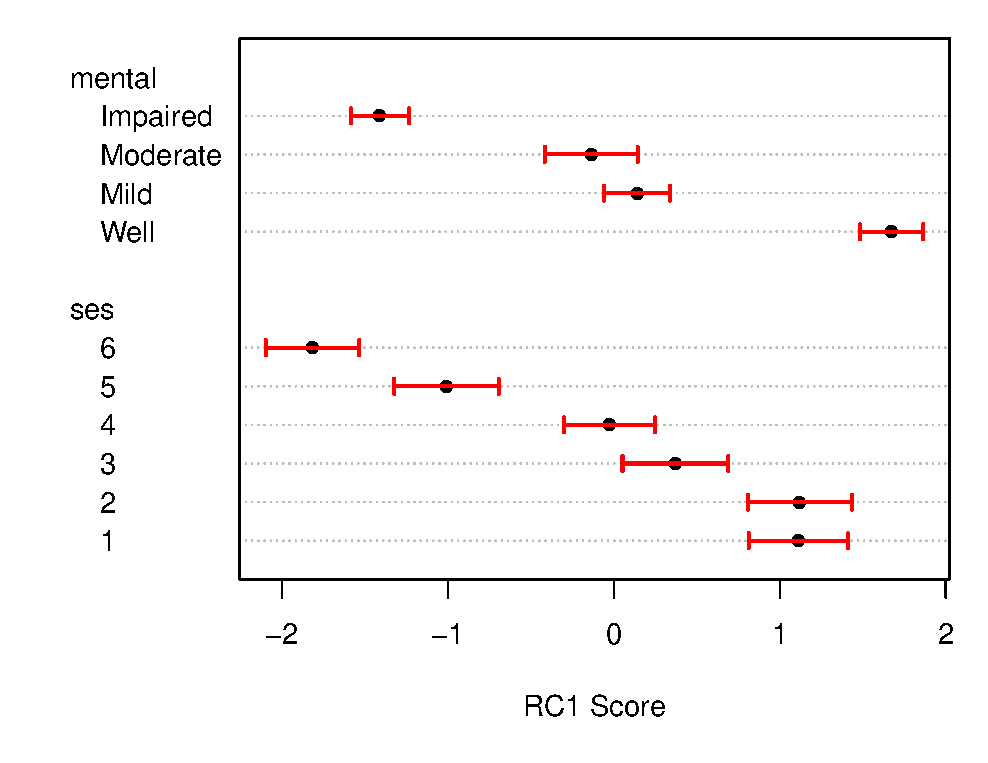
\includegraphics[width=.8\textwidth]{ch08/fig/mental-RC1}
\caption{Dotchart of the scaled category scores for the RC(1) model fit
the mental health data.  Error bars show $\pm 1$ standard error.}
\label{fig:mental-RC1}
\end{figure}

To create this plot, first combine the row and column scores
in a data frame, and add columns \code{lower, upper}
corresponding to $\pm 1$ standard error (or some other multiple).

\begin{knitrout}
\definecolor{shadecolor}{rgb}{1, 0.961, 0.933}\color{fgcolor}\begin{kframe}
\begin{alltt}
\hlstd{scores} \hlkwb{<-} \hlkwd{rbind}\hlstd{(alpha, beta)}
\hlstd{scores} \hlkwb{<-} \hlkwd{cbind}\hlstd{(scores,}
                \hlkwc{factor}\hlstd{=}\hlkwd{c}\hlstd{(}\hlkwd{rep}\hlstd{(}\hlstr{"mental"}\hlstd{,} \hlnum{4}\hlstd{),} \hlkwd{rep}\hlstd{(}\hlstr{"ses"}\hlstd{,} \hlnum{6}\hlstd{)) )}
\hlkwd{rownames}\hlstd{(scores)} \hlkwb{<-} \hlkwd{c}\hlstd{(}\hlkwd{levels}\hlstd{(Mental}\hlopt{$}\hlstd{mental),} \hlkwd{levels}\hlstd{(Mental}\hlopt{$}\hlstd{ses))}
\hlstd{scores}\hlopt{$}\hlstd{lower} \hlkwb{<-} \hlstd{scores[,}\hlnum{1}\hlstd{]}\hlopt{-}\hlstd{scores[,}\hlnum{2}\hlstd{]}
\hlstd{scores}\hlopt{$}\hlstd{upper} \hlkwb{<-} \hlstd{scores[,}\hlnum{1}\hlstd{]}\hlopt{+}\hlstd{scores[,}\hlnum{2}\hlstd{]}
\hlstd{scores}
\end{alltt}
\begin{verbatim}
##           Estimate Std. Error factor     lower    upper
## Well      1.673783    0.19043 mental  1.483355  1.86421
## Mild      0.140087    0.20018 mental -0.060093  0.34027
## Moderate -0.136688    0.27948 mental -0.416167  0.14279
## Impaired -1.410547    0.17418 mental -1.584728 -1.23636
## 1         1.111361    0.29921    ses  0.812150  1.41057
## 2         1.120459    0.31422    ses  0.806243  1.43467
## 3         0.370752    0.31915    ses  0.051601  0.68990
## 4        -0.027006    0.27328    ses -0.300281  0.24627
## 5        -1.009480    0.31470    ses -1.324179 -0.69478
## 6        -1.816647    0.28095    ses -2.097600 -1.53569
\end{verbatim}
\end{kframe}
\end{knitrout}
The dotchart shown in \figref{fig:mental-RC1} is then a plot of
\code{Estimate}, grouped by \code{factor}, with arrows
showing the range of \code{lower} to \code{upper} for each
parameter.
\begin{knitrout}
\definecolor{shadecolor}{rgb}{1, 0.961, 0.933}\color{fgcolor}\begin{kframe}
\begin{alltt}
\hlkwd{with}\hlstd{(scores, \{}
  \hlkwd{dotchart}\hlstd{(Estimate,} \hlkwc{groups}\hlstd{=factor,} \hlkwc{labels}\hlstd{=}\hlkwd{rownames}\hlstd{(scores),}
           \hlkwc{cex}\hlstd{=}\hlnum{1.2}\hlstd{,} \hlkwc{pch}\hlstd{=}\hlnum{16}\hlstd{,} \hlkwc{xlab}\hlstd{=}\hlstr{"RC1 Score"}\hlstd{,}
           \hlkwc{xlim}\hlstd{=}\hlkwd{c}\hlstd{(}\hlkwd{min}\hlstd{(lower),} \hlkwd{max}\hlstd{(upper)))}
  \hlkwd{arrows}\hlstd{(lower,} \hlkwd{c}\hlstd{(}\hlnum{8}\hlopt{+}\hlstd{(}\hlnum{1}\hlopt{:}\hlnum{4}\hlstd{),} \hlnum{1}\hlopt{:}\hlnum{6}\hlstd{), upper,} \hlkwd{c}\hlstd{(}\hlnum{8}\hlopt{+}\hlstd{(}\hlnum{1}\hlopt{:}\hlnum{4}\hlstd{),} \hlnum{1}\hlopt{:}\hlnum{6}\hlstd{),}
         \hlkwc{col}\hlstd{=}\hlstr{"red"}\hlstd{,} \hlkwc{angle}\hlstd{=}\hlnum{90}\hlstd{,} \hlkwc{length}\hlstd{=}\hlnum{.05}\hlstd{,} \hlkwc{code}\hlstd{=}\hlnum{3}\hlstd{,} \hlkwc{lwd}\hlstd{=}\hlnum{2}\hlstd{)}
  \hlstd{\})}
\end{alltt}
\end{kframe}
\end{knitrout}
In this plot, the main substantive difference from the $L \times L$
model is in the spacing of the lowest two categories of \code{ses}
and the middle two categories of \code{mental} which are not
seen to differ in the RC1 model.

The coefficients in the  \code{RC2} model can also be plotted (in a 2D plot)
by extracting the coefficients from the \class{gnm} object and
reshaping them to 2-column matrices.  The function \func{pickCoef}
is handy here to get the indices of a subset of parameters by
matching a pattern in their names. \TODO{Maybe delete some of this, in favor of
using \pkg{logmult}.}

\begin{knitrout}
\definecolor{shadecolor}{rgb}{1, 0.961, 0.933}\color{fgcolor}\begin{kframe}
\begin{alltt}
\hlstd{alpha} \hlkwb{<-} \hlkwd{coef}\hlstd{(RC2)[}\hlkwd{pickCoef}\hlstd{(RC2,} \hlstr{"[.]mental"}\hlstd{)]}
\hlstd{alpha} \hlkwb{<-} \hlkwd{matrix}\hlstd{(alpha,} \hlkwc{ncol}\hlstd{=}\hlnum{2}\hlstd{)}
\hlkwd{rownames}\hlstd{(alpha)} \hlkwb{<-} \hlkwd{levels}\hlstd{(Mental}\hlopt{$}\hlstd{mental)}
\hlkwd{colnames}\hlstd{(alpha)} \hlkwb{<-} \hlkwd{c}\hlstd{(}\hlstr{"Dim1"}\hlstd{,} \hlstr{"Dim2"}\hlstd{)}
\hlstd{alpha}
\end{alltt}
\begin{verbatim}
##               Dim1      Dim2
## Well      0.202004  0.399912
## Mild      0.017298  0.062629
## Moderate -0.135466  0.322385
## Impaired -0.099260 -0.455564
\end{verbatim}
\begin{alltt}
\hlstd{beta} \hlkwb{<-} \hlkwd{coef}\hlstd{(RC2)[}\hlkwd{pickCoef}\hlstd{(RC2,} \hlstr{"[.]ses"}\hlstd{)]}
\hlstd{beta} \hlkwb{<-} \hlkwd{matrix}\hlstd{(beta,} \hlkwc{ncol}\hlstd{=}\hlnum{2}\hlstd{)}
\hlkwd{rownames}\hlstd{(beta)} \hlkwb{<-} \hlkwd{levels}\hlstd{(Mental}\hlopt{$}\hlstd{ses)}
\hlkwd{colnames}\hlstd{(beta)} \hlkwb{<-} \hlkwd{c}\hlstd{(}\hlstr{"Dim1"}\hlstd{,} \hlstr{"Dim2"}\hlstd{)}
\hlstd{beta}
\end{alltt}
\begin{verbatim}
##       Dim1     Dim2
## 1  0.94513  0.38381
## 2  0.86321  0.42585
## 3  0.33210  0.14705
## 4  0.59750 -0.20052
## 5 -0.28284 -0.46276
## 6 -1.96825 -0.41681
\end{verbatim}
\end{kframe}
\end{knitrout}

The simple, unweighted scaling to mean 0, variance 1 can be obtained with \func{scale}:
\begin{knitrout}
\definecolor{shadecolor}{rgb}{1, 0.961, 0.933}\color{fgcolor}\begin{kframe}
\begin{alltt}
\hlstd{alpha} \hlkwb{<-} \hlkwd{scale}\hlstd{(alpha)}
\hlstd{beta} \hlkwb{<-} \hlkwd{scale}\hlstd{(beta)}
\end{alltt}
\end{kframe}
\end{knitrout}
\noindent Alternatively, the marginal-weighted scaling of \eqref{eq:RC-constraints}
is obtained by centering at the weighted mean and dividing by the weighted
sum of squares.  We use this scaling here.
\begin{knitrout}
\definecolor{shadecolor}{rgb}{1, 0.961, 0.933}\color{fgcolor}\begin{kframe}
\begin{alltt}
\hlstd{alpha} \hlkwb{<-} \hlkwd{apply}\hlstd{(alpha,} \hlnum{2}\hlstd{,} \hlkwa{function}\hlstd{(}\hlkwc{x}\hlstd{) x} \hlopt{-} \hlkwd{sum}\hlstd{(x}\hlopt{*}\hlstd{rowProbs))}
\hlstd{alpha} \hlkwb{<-} \hlkwd{apply}\hlstd{(alpha,} \hlnum{2}\hlstd{,} \hlkwa{function}\hlstd{(}\hlkwc{x}\hlstd{) x}\hlopt{/}\hlkwd{sqrt}\hlstd{(}\hlkwd{sum}\hlstd{(x}\hlopt{^}\hlnum{2} \hlopt{*} \hlstd{rowProbs)))}
\hlstd{beta} \hlkwb{<-} \hlkwd{apply}\hlstd{(beta,} \hlnum{2}\hlstd{,} \hlkwa{function}\hlstd{(}\hlkwc{x}\hlstd{) x} \hlopt{-} \hlkwd{sum}\hlstd{(x}\hlopt{*}\hlstd{colProbs))}
\hlstd{beta} \hlkwb{<-} \hlkwd{apply}\hlstd{(beta,} \hlnum{2}\hlstd{,} \hlkwa{function}\hlstd{(}\hlkwc{x}\hlstd{) x}\hlopt{/}\hlkwd{sqrt}\hlstd{(}\hlkwd{sum}\hlstd{(x}\hlopt{^}\hlnum{2} \hlopt{*} \hlstd{colProbs)))}
\end{alltt}
\end{kframe}
\end{knitrout}
To plot these category scores, first combine them into a single data frame,
\begin{knitrout}
\definecolor{shadecolor}{rgb}{1, 0.961, 0.933}\color{fgcolor}\begin{kframe}
\begin{alltt}
\hlstd{scores} \hlkwb{<-} \hlkwd{data.frame}\hlstd{(}\hlkwd{rbind}\hlstd{(alpha,beta))}
\hlstd{scores}\hlopt{$}\hlstd{factor} \hlkwb{<-} \hlkwd{c}\hlstd{(}\hlkwd{rep}\hlstd{(}\hlstr{"mental"}\hlstd{,} \hlnum{4}\hlstd{),} \hlkwd{rep}\hlstd{(}\hlstr{"ses"}\hlstd{,} \hlnum{6}\hlstd{))}
\hlstd{scores}\hlopt{$}\hlstd{probs} \hlkwb{<-} \hlkwd{c}\hlstd{(rowProbs, colProbs)}
\hlstd{scores}
\end{alltt}
\begin{verbatim}
##              Dim1       Dim2 factor   probs
## Well      1.79233  1.0814056 mental 0.18494
## Mild      0.22465  0.0076701 mental 0.36265
## Moderate -1.07194  0.8345990 mental 0.21807
## Impaired -0.76464 -1.6419892 mental 0.23434
## 1         0.84450  1.1862716    ses 0.15783
## 2         0.75528  1.3079993    ses 0.14759
## 3         0.17681  0.5007482    ses 0.17289
## 4         0.46588 -0.5056279    ses 0.23133
## 5        -0.49295 -1.2649089    ses 0.15964
## 6        -2.32862 -1.1318698    ses 0.13072
\end{verbatim}
\end{kframe}
\end{knitrout}
\begin{figure}[!htb]
\centering
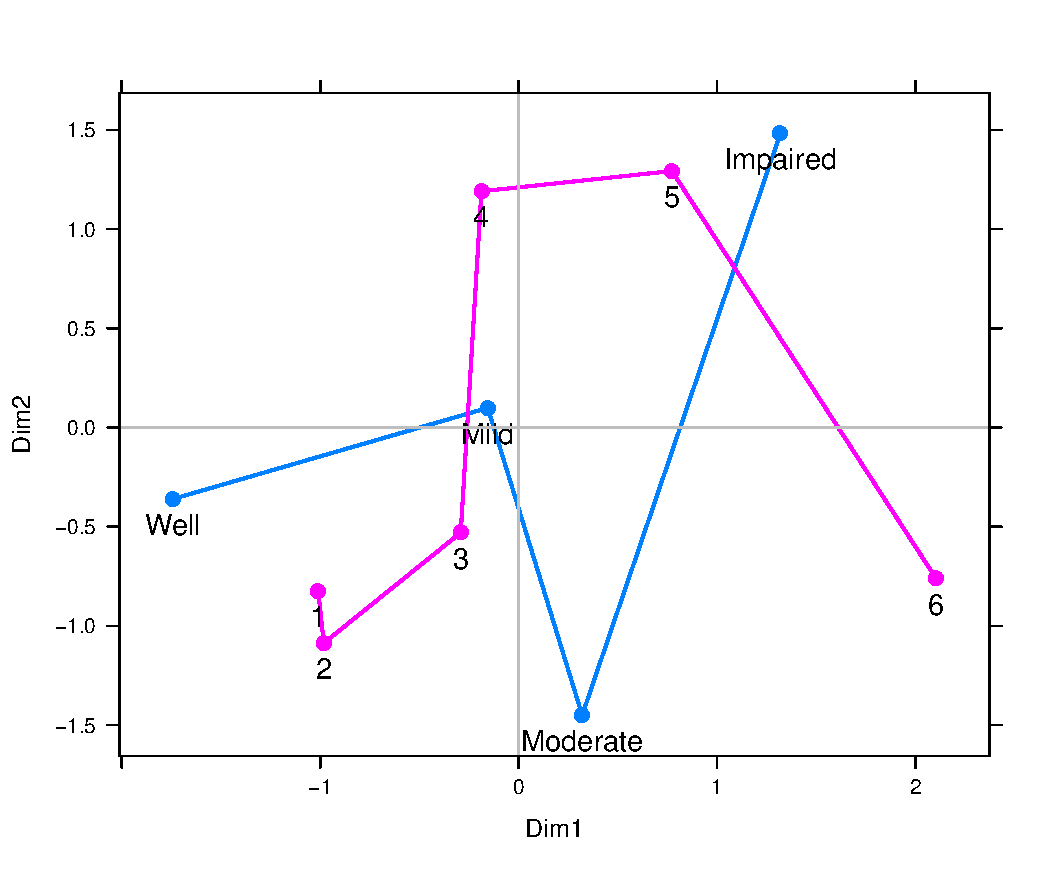
\includegraphics[width=.7\textwidth]{ch08/fig/mental-RC2}
\caption{Scaled category scores for the RC(2) model fit
the mental health data.}
\label{fig:mental-RC2}
\end{figure}

Then, we use \func{xyplot} to plot the scores on \code{Dim2} against \code{Dim1},
with separate lines and colors for the two factors.  The resulting plot is
shown in \figref{fig:mental-RC2}.
\begin{knitrout}
\definecolor{shadecolor}{rgb}{1, 0.961, 0.933}\color{fgcolor}\begin{kframe}
\begin{alltt}
\hlkwd{library}\hlstd{(lattice)}
\hlkwd{xyplot}\hlstd{(Dim2} \hlopt{~} \hlstd{Dim1,} \hlkwc{groups}\hlstd{=factor,} \hlkwc{data}\hlstd{=scores,} \hlkwc{type}\hlstd{=}\hlstr{"b"}\hlstd{,}
       \hlkwc{cex}\hlstd{=}\hlnum{1.3}\hlstd{,} \hlkwc{pch}\hlstd{=}\hlnum{16}\hlstd{,} \hlkwc{lwd}\hlstd{=}\hlnum{2}\hlstd{,} \hlkwc{aspect}\hlstd{=}\hlstr{"iso"}\hlstd{,}
       \hlkwc{panel}\hlstd{=}\hlkwa{function}\hlstd{(}\hlkwc{x}\hlstd{,} \hlkwc{y}\hlstd{,} \hlkwc{...}\hlstd{) \{}
          \hlkwd{panel.xyplot}\hlstd{(x, y, ...)}
          \hlkwd{panel.text}\hlstd{(}\hlkwc{x}\hlstd{=x,} \hlkwc{y}\hlstd{=y,} \hlkwc{labels}\hlstd{=}\hlkwd{rownames}\hlstd{(scores),} \hlkwc{pos}\hlstd{=}\hlnum{1}\hlstd{,} \hlkwc{cex}\hlstd{=}\hlnum{1.2}\hlstd{)}
          \hlkwd{panel.abline}\hlstd{(}\hlkwc{h}\hlstd{=}\hlnum{0}\hlstd{,} \hlkwc{col}\hlstd{=}\hlstr{"gray"}\hlstd{)}
          \hlkwd{panel.abline}\hlstd{(}\hlkwc{v}\hlstd{=}\hlnum{0}\hlstd{,} \hlkwc{col}\hlstd{=}\hlstr{"gray"}\hlstd{)}
          \hlstd{\}}
  \hlstd{)}
\end{alltt}
\end{kframe}
\end{knitrout}
The patterns of the row and column category scores here are quite similar to the
2D \ca solution shown in \figref{fig:ca-mental-plot}.  The main difference is in the
relative scaling of the axes.  In \figref{fig:mental-RC2}, the variances of the
two dimensions are equated; in the \ca plot, the axes are scaled in relation to
their contributions to Pearson \chisq, allowing an interpretation of distance between
points in terms of \chisq-distance.

\end{Example}

\subsubsection[Using logmult]{Using \pkg{logmult}}

From the previous example, you can see that it takes a fair bit of work to extract the
coefficients from \class{gnm} objects and carry out the scaling necessary for informative
plots.  Much of this effort is now performed by the \Rpackage{logmult} with several
convenience functions that do the heavy lifting.

\begin{description}
  \item[\func{rc}] fits the class of RC(M) models, allowing an argument \code{nd} to
  specify the number of dimensions, and also providing for
  standard errors
  estimated using jackknife and bootstrap methods \citep{MilanWhittaker:1995},
  which are computationally intensive.  For square tables, a \code{symmetric}
  argument constrains the row and column scores to be equal, and a
  \code{diagonal} option fits parameters for each diagonal cell,
  providing for models of quasi-independence and quasi-symmetry (see \secref{sec:loglin-square}).

  It returns an object of class \class{rc} with the components of the
  \class{gnm} object. An \code{assoc} component is also returned, containing
  the normalized association parameters for the categories.
  \item[\func{rcL}] fits extensions of RC models to tables with multiple layers,
  called RC(M)-L models by \cite{Wong:2010}.
%   \item[\func{assoc }] performs the steps to identify the
%   log-multiplicative association scores from over-parameterized \class{gnm} models.%
%   \footnote{
%   This conflicts with \func{assoc} for association plots in the
%   \Rpackage{vcd}, so we use this here as \code{logmult::assoc}.
%   }
  \item[\func{plot.rc}] is a plot method for visualizing scores for RC(M) models
  in two selected dimensions. Among other options, it can plot confidence
  ellipses for the category scores, using the estimated covariance matrix
  (assuming a normal distribution of the category scores). The plot method
  returns (invisibly) the coordinates of the scores as plotted, facilitating
  additional plot annotation.
\end{description}


\begin{Example}[mental6]{Mental impairment and parents' SES}
Here we use \func{rc} to estimate the RC(1) and RC(2) models for the
\data{Mental} data.  In contrast to \func{gnm}, which has a
formula interface for a \code{data} argument,
\func{rc} requires the input in the form of a two-way table,
given here as \code{mental.tab}.
\begin{knitrout}
\definecolor{shadecolor}{rgb}{1, 0.961, 0.933}\color{fgcolor}\begin{kframe}
\begin{alltt}
\hlkwd{library}\hlstd{(logmult)}
\hlstd{rc1} \hlkwb{<-} \hlkwd{rc}\hlstd{(mental.tab,} \hlkwc{verbose}\hlstd{=}\hlnum{FALSE}\hlstd{,} \hlkwc{weighting}\hlstd{=}\hlstr{"marginal"}\hlstd{,}
          \hlkwc{se}\hlstd{=}\hlstr{"jackknife"}\hlstd{)}
\hlstd{rc2} \hlkwb{<-} \hlkwd{rc}\hlstd{(mental.tab,} \hlkwc{verbose}\hlstd{=}\hlnum{FALSE}\hlstd{,} \hlkwc{weighting}\hlstd{=}\hlstr{"marginal"}\hlstd{,} \hlkwc{nd}\hlstd{=}\hlnum{2}\hlstd{,}
          \hlkwc{se}\hlstd{=}\hlstr{"jackknife"}\hlstd{)}
\end{alltt}
\end{kframe}
\end{knitrout}
\noindent The option \code{weighting="marginal"} gives the marginally-weighted solution
and \code{se="jackknife"} estimates the covariance matrix using the
leave-one-out jackknife.%
\footnote{
\citet{BeckerClogg:1989} recommend using unweighted solutions, \code{weighting="none"}
(they call them ``uniformly weighted'')
to preserve independence of inferences about association and marginal effects
and estimates of the intrinsic association parameters, $\gamma_k$.
That choice makes very little difference in the plots for this example,
but the $\gamma_k$ parameters are affected considerably.
}

A plot of the scaled category scores similar to \figref{fig:mental-RC2},
with 1 standard error confidence ellipses
(making them comparable to the 1D solution shown in \figref{fig:mental-RC1})
but no connecting lines
can then be easily produced with
the \func{plot} method for \class{rc} objects.
\begin{knitrout}
\definecolor{shadecolor}{rgb}{1, 0.961, 0.933}\color{fgcolor}\begin{kframe}
\begin{alltt}
\hlstd{coords}  \hlkwb{<-} \hlkwd{plot}\hlstd{(rc2,} \hlkwc{conf.ellipses}\hlstd{=}\hlnum{0.68}\hlstd{,} \hlkwc{cex}\hlstd{=}\hlnum{1.5}\hlstd{,} \hlkwc{rev.axes}\hlstd{=}\hlkwd{c}\hlstd{(}\hlnum{TRUE}\hlstd{,} \hlnum{FALSE}\hlstd{))}
\end{alltt}
\end{kframe}
\end{knitrout}
\noindent The orientation of the axes is arbitrary in RC(M) models, so the horizontal
axis is reversed here to conform with \figref{fig:mental-RC2}.

This produces (in \figref{fig:mental-logmult-rc2}) a
symmetric \IX{biplot} in which the scaled
coordinates of points for rows ($\alpha_{ik}$) and columns ($\beta_{jk}$)
on both axes are the product of normalized scores and the square root of the intrinsic association coefficient ($\gamma_k$) corresponding to each dimension.

\begin{figure}[!htb]
\centering
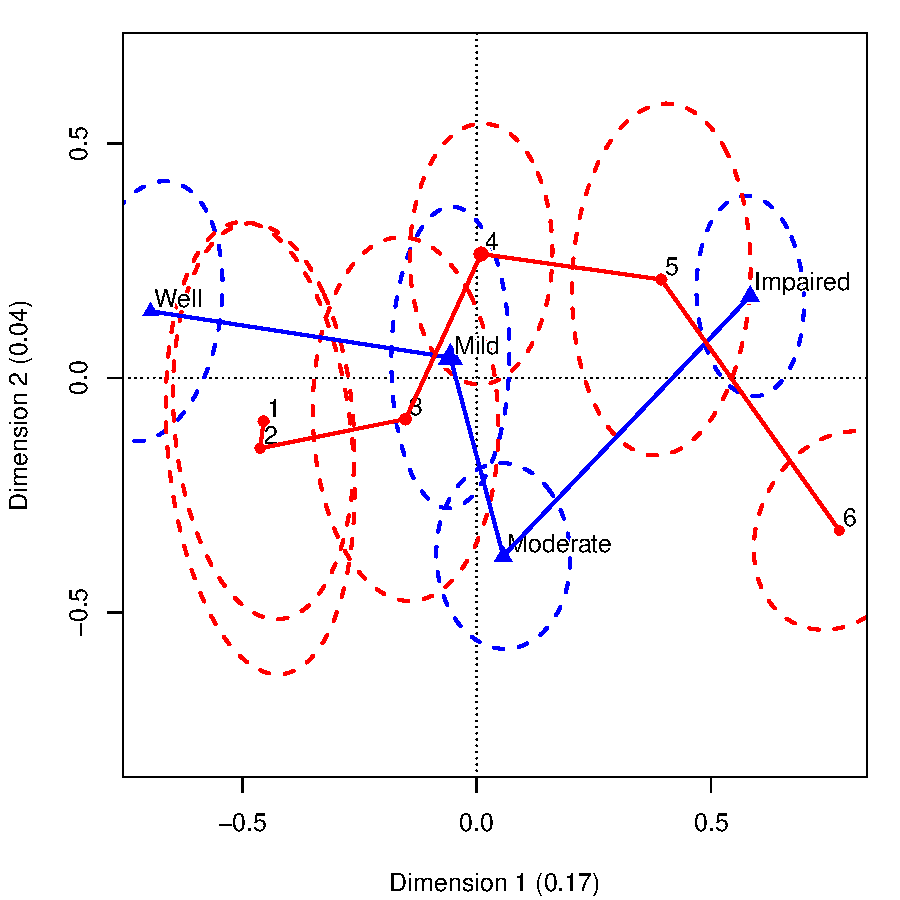
\includegraphics[width=.7\textwidth]{ch08/fig/mental-logmult-rc2}
\caption{Scaled category scores for the RC(2) model fit
and plotted using the \Rpackage{logmult}.  The 68\%
confidence ellipses correspond to bivariate
$\pm 1$  confidence
intervals for the category parameters.}
\label{fig:mental-logmult-rc2}
\end{figure}

Such plots can be customized using the category coordinates (\code{coords})
returned by the \func{plot} method.
As in other biplots, joining the row and column points
by lines (sorted by the first dimension) makes it easier to see their
relationships across the two dimensions.  The following code
draws the lines shown in \figref{fig:mental-logmult-rc2}.
\begin{knitrout}
\definecolor{shadecolor}{rgb}{1, 0.961, 0.933}\color{fgcolor}\begin{kframe}
\begin{alltt}
\hlstd{scores} \hlkwb{<-} \hlkwd{rbind}\hlstd{(coords}\hlopt{$}\hlstd{row, coords}\hlopt{$}\hlstd{col)}
\hlkwd{lines}\hlstd{(scores[}\hlnum{1}\hlopt{:}\hlnum{4}\hlstd{,],} \hlkwc{col}\hlstd{=}\hlstr{"blue"}\hlstd{,} \hlkwc{lwd}\hlstd{=}\hlnum{2}\hlstd{)}
\hlkwd{lines}\hlstd{(scores[}\hlopt{-}\hlstd{(}\hlnum{1}\hlopt{:}\hlnum{4}\hlstd{),],} \hlkwc{col}\hlstd{=}\hlstr{"red"}\hlstd{,} \hlkwc{lwd}\hlstd{=}\hlnum{2}\hlstd{)}
\end{alltt}
\end{kframe}
\end{knitrout}

We saw earlier that there was not strong evidence supporting the need for a
second RC dimension to describe the relationship between mental health and SES.
This is apparent in the sizes of the confidence ellipses, which overlap much more along
Dimension 2 than Dimension 1.
\end{Example}

 
\section{Square tables}\label{sec:loglin-square}

%\section{Square tables}\label{sec:loglin-square}

Square tables, where the row and column variables have the same categories
comprise an important special case for \loglin models that can account
for associations more parsimoniously than the saturated model.
Some examples are the data on visual acuity in \exref{ex:vision1},
categorical ratings of therapy clients by two observers,
and mobility tables, tracking the occupational categories
between generations in the same families or migration
tables, giving movement of people between regions.
The latter topics has been important in sociological and geographic
research
and has spurred the development of a wide range of specialized
\loglin models for this purpose.

\subsection{Quasi-independence, symmetry, quasi-symmetry and topological models}\label{sec:sq-quasi}

In many square tables, such as the \data{Vision} data, independence is
not a credible hypothesis because the diagonal cells, representing
equal values of the row and column variables tend to be very large
and often contribute most of the lack of fit.
A substantively more interesting hypothesis is whether the table
exhibits independence, ignoring the diagonal cells. This
leads to what is called the \term{quasi-independence model},
that specifies independence only in the off-diagonal cells.

For a two-way table, quasi-independence can be expressed as
\begin{equation*}
 \pi_{ij} = \pi_{i+} \pi_{+j} \quad\quad \mbox{for } i\ne j
\end{equation*}
or in \loglin form as
\begin{equation*}
 \log m_{ij} = \mu + \lambda_i^A + \lambda_j^B + \delta_i I(i=j)
 \period
\end{equation*}
This model effectively adds one parameter, $\delta_i$, for each main diagonal cell
which fits those frequencies perfectly.


Another hypothesis of substantive interest for square tables,
particularly those concerning occupational and geographical
mobility is that the joint distribution of row and column
variables is symmetric, that is,
$\pi_{ij} = \pi_{ji}$ for all $i \ne j$.
For example, this \term{symmetry model} (S)
asserts that sons are as likely to
move from their father's occupation $i$ to another, $j$,
as the reverse.
This form of symmetry is quite strong, because it also implies
\term{marginal homogeneity} (MH),
that the marginal probabilities of the row and column variables
are equal,
$\pi_{i+} = \sum_j \pi_{ij} = \sum_j \pi_{ji} = \pi_{+i}$
for all $i$.

To separate marginal homogeneity from symmetry of the association terms
per se, the model of \term{quasi-symmetry} (QS)
uses the standard
main-effect terms in the \loglin model,
\begin{equation}\label{eq:quasi-symm}
 \log m_{ij} = \mu + \lambda_i^A + \lambda_j^B + \lambda_{ij}
 \comma
\end{equation}
where $\lambda_{ij} = \lambda_{ji}$.  It can be shown \citep{caus:1966} that
\begin{eqnarray*}
\mbox{symmetry} & = & \mbox{quasi-symmetry} + \mbox{marginal homogeneity} \\
      \GSQ (S)  & = & \GSQ (QS) + \GSQ (MH)
\end{eqnarray*}
where $\GSQ (MH)$ is defined by the \LR test of the difference between the
S and QS models,
\begin{equation}\label{eq:mh}
\GSQ (MH) \equiv \GSQ (S \given QS) =  \GSQ (S) - \GSQ (QS) \period
\end{equation}

The \Rpackage{gnm} provides several model building convenience functions that
facilitate fitting these and related models:
\begin{itemize*}
 \item \code{Diag(row, col, ...)} constructs a diagonals association
 factor for two (or more)
 factors with integer levels where the original factors are equal, and \code{"."} otherwise.
 \item \code{Symm(row, col, ...)} constructs an association
 factor giving equal levels to
 sets of symmetric cells.  The QS model is specified using \code{Diag() + Symm()}.
 \item \code{Topo(row, col, ..., spec)} creates an association factor for two or more
 factors, as specified by an array of levels, which may be arbitrarily structured.
 Both \func{Diag} and \func{Symm} factors are special cases of \func{Topo}.
\end{itemize*}

The factor levels representing these association effects for a $4 \times 4$ table
are shown below by their unique values in each array.
\begin{equation*}
% latex table generated in R 3.0.1 by xtable 1.7-3 package
% Mon Jun 02 11:13:33 2014
\small
\mbox{Diag}_{4 \times 4} =
\left[
\begin{array}{rrrr}
  1 & . & . & . \\ 
  . & 2 & . & . \\ 
  . & . & 3 & . \\ 
  . & . & . & 4  
\end{array}
\right]
\quad
%
\mbox{Symm}_{4 \times 4} =
\left[
\begin{array}{rrrr}
  11 & 12 & 13 & 14 \\ 
  12 & 22 & 23 & 24 \\ 
  13 & 23 & 33 & 34 \\ 
  14 & 24 & 34 & 44  
\end{array}
\right]
\quad
%
\mbox{Topo}_{4 \times 4} =
\left[
\begin{array}{rrrr}
  2 & 3 & 4 & 4 \\ 
  3 & 3 & 4 & 4 \\ 
  4 & 4 & 5 & 5 \\ 
  4 & 4 & 5 & 1 
\end{array}
\right]
\end{equation*}



\begin{Example}[vision-glm]{Visual acuity}
\exref{ex:vision1} presented the data on tests of visual acuity in the left and right eyes
of a large sample of women working in the Royal Ordnance factories in World War II.
A sieve diagram (\figref{fig:VA-sieve2}) showed that, as expected, most women had the
same acuity in both eyes, but the off-diagonal cells had a pattern suggesting some form
of symmetry.

The data set \data{VisualAcuity} contains data for both men and women in frequency form
and for this example we subset this to include only the $4 \times 4$ table for women.
\begin{knitrout}
\definecolor{shadecolor}{rgb}{1, 0.961, 0.933}\color{fgcolor}\begin{kframe}
\begin{alltt}
\hlkwd{data}\hlstd{(}\hlstr{"VisualAcuity"}\hlstd{,} \hlkwc{package}\hlstd{=}\hlstr{"vcd"}\hlstd{)}
\hlstd{women} \hlkwb{<-} \hlkwd{subset}\hlstd{(VisualAcuity, gender}\hlopt{==}\hlstr{"female"}\hlstd{,} \hlkwc{select}\hlstd{=}\hlopt{-}\hlstd{gender)}
\end{alltt}
\end{kframe}
\end{knitrout}
The four basic models of independence, quasi-independence, symmetry and quasi-symmetry
for square tables are fit as shown below.  We use \func{update} to highlight
the relations among these models in two pairs.
\begin{knitrout}
\definecolor{shadecolor}{rgb}{1, 0.961, 0.933}\color{fgcolor}\begin{kframe}
\begin{alltt}
\hlcom{#library(vcdExtra)}
\hlstd{indep} \hlkwb{<-} \hlkwd{glm}\hlstd{(Freq} \hlopt{~} \hlstd{right} \hlopt{+} \hlstd{left,}  \hlkwc{data} \hlstd{= women,} \hlkwc{family} \hlstd{= poisson)}
\hlstd{quasi} \hlkwb{<-} \hlkwd{update}\hlstd{(indep, .} \hlopt{~} \hlstd{.} \hlopt{+} \hlkwd{Diag}\hlstd{(right, left))}
\hlcom{# @}
\hlcom{# <<vision-glm3>>=}
\hlstd{symm} \hlkwb{<-} \hlkwd{glm}\hlstd{(Freq} \hlopt{~} \hlkwd{Symm}\hlstd{(right, left),} \hlkwc{data} \hlstd{= women,} \hlkwc{family} \hlstd{= poisson)}
\hlstd{qsymm} \hlkwb{<-} \hlkwd{update}\hlstd{(symm, .} \hlopt{~} \hlstd{right} \hlopt{+} \hlstd{left} \hlopt{+} \hlstd{.)}
\end{alltt}
\end{kframe}
\end{knitrout}
The brief summary of goodness of fit of these models below shows that
the QS model fits reasonably well, but none of the others do by
\LR tests or AIC or BIC.
\begin{knitrout}
\definecolor{shadecolor}{rgb}{1, 0.961, 0.933}\color{fgcolor}\begin{kframe}
\begin{alltt}
\hlstd{vcdExtra::}\hlkwd{Summarise}\hlstd{(indep, quasi, symm, qsymm)}
\end{alltt}
\begin{verbatim}
## Likelihood summary table:
##        AIC  BIC LR Chisq Df Pr(>Chisq)    
## indep 6803 6808     6672  9     <2e-16 ***
## quasi  338  347      199  5     <2e-16 ***
## symm   157  164       19  6     0.0038 ** 
## qsymm  151  161        7  3     0.0638 .  
## ---
## Signif. codes:  0 '***' 0.001 '**' 0.01 '*' 0.05 '.' 0.1 ' ' 1
\end{verbatim}
\end{kframe}
\end{knitrout}
Beyond just saying that the QS model fits best, the reasons \emph{why} it does
can be seen in mosaic displays.  \figref{fig:vision-mosaics} compares the
mosaics for the models of quasi-independence
(accounting only for the diagonal cells)
and quasi-symmetry (also accounting for symmetry).  It can be seen in the left
panel that the non-diagonal associations are largely symmetric, and also that
when they differ, visual acuity in the two eyes are most likely to differ by
only one eye grade.

\begin{knitrout}
\definecolor{shadecolor}{rgb}{1, 0.961, 0.933}\color{fgcolor}\begin{kframe}
\begin{alltt}
\hlstd{labs} \hlkwb{<-} \hlkwd{c}\hlstd{(}\hlstr{"High"}\hlstd{,} \hlstr{"2"}\hlstd{,} \hlstr{"3"}\hlstd{,} \hlstr{"Low"}\hlstd{)}
\hlstd{largs} \hlkwb{<-} \hlkwd{list}\hlstd{(}\hlkwc{set_varnames} \hlstd{=} \hlkwd{c}\hlstd{(}\hlkwc{right}\hlstd{=}\hlstr{"Right eye grade"}\hlstd{,}
                               \hlkwc{left}\hlstd{=}\hlstr{"Left eye grade"}\hlstd{),}
              \hlkwc{set_labels}\hlstd{=}\hlkwd{list}\hlstd{(}\hlkwc{right}\hlstd{=labs,} \hlkwc{left}\hlstd{=labs))}
\hlkwd{mosaic}\hlstd{(quasi,} \hlopt{~}\hlstd{right} \hlopt{+} \hlstd{left,} \hlkwc{residuals_type}\hlstd{=}\hlstr{"rstandard"}\hlstd{,}
       \hlkwc{gp}\hlstd{=shading_Friendly,}
       \hlkwc{labeling_args}\hlstd{=largs,}
       \hlkwc{main}\hlstd{=}\hlstr{"Quasi-Independence (women)"}\hlstd{)}
\hlkwd{mosaic}\hlstd{(qsymm,} \hlopt{~}\hlstd{right} \hlopt{+} \hlstd{left,} \hlkwc{residuals_type}\hlstd{=}\hlstr{"rstandard"}\hlstd{,}
       \hlkwc{gp}\hlstd{=shading_Friendly,}
       \hlkwc{labeling_args}\hlstd{=largs,}
       \hlkwc{main}\hlstd{=}\hlstr{"Quasi-Symmetry (women)"}\hlstd{)}
\end{alltt}
\end{kframe}\begin{figure}[!htbp]


\centerline{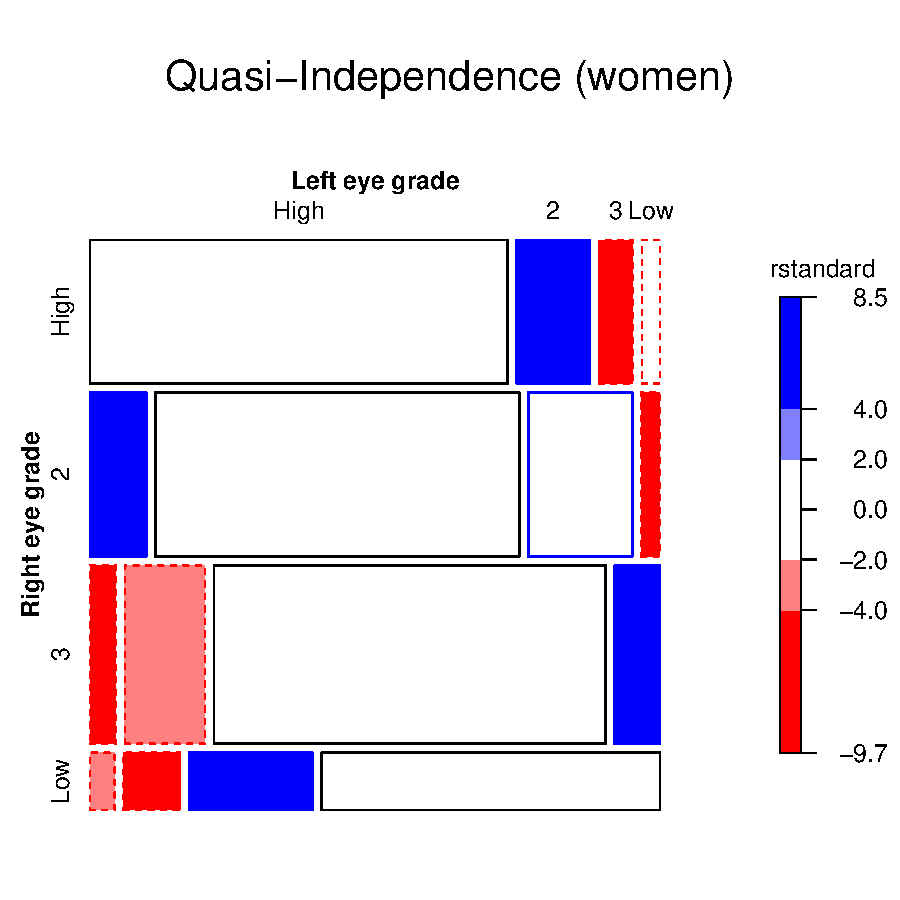
\includegraphics[width=.49\textwidth]{ch08/fig/vision-mosaics-1} 
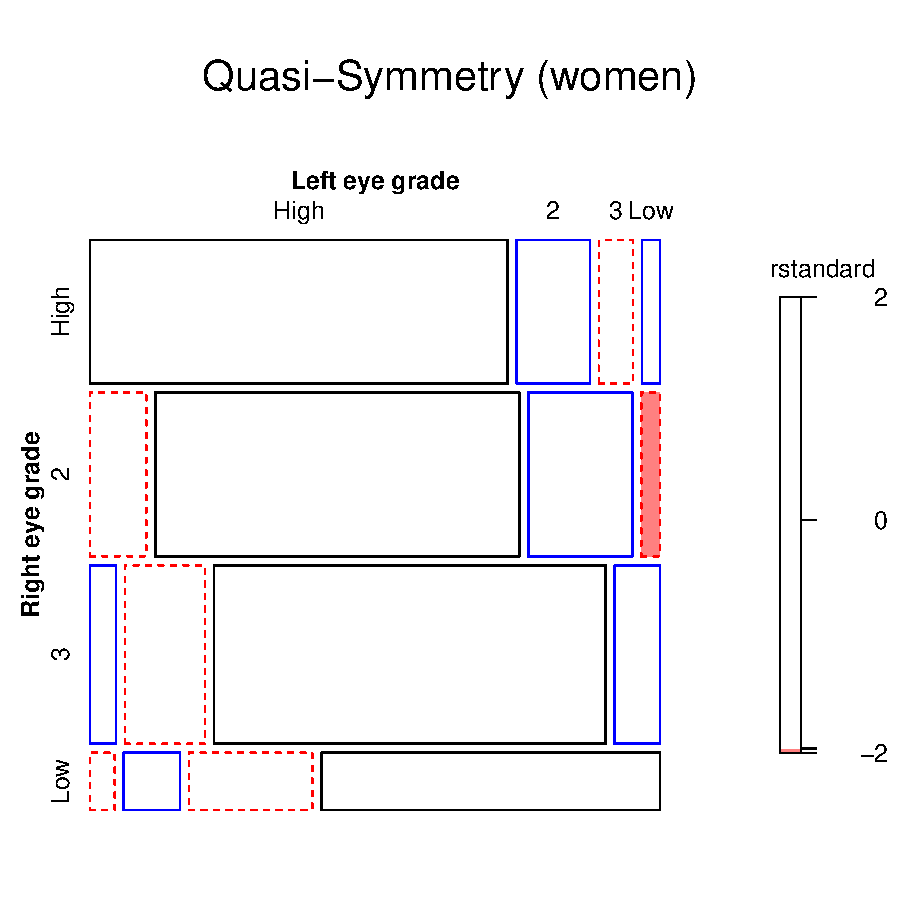
\includegraphics[width=.49\textwidth]{ch08/fig/vision-mosaics-2} }

\caption[Mosaic displays comparing the models of quasi-independence and quasi-symmetry for visual acuity in women]{Mosaic displays comparing the models of quasi-independence and quasi-symmetry for visual acuity in women.\label{fig:vision-mosaics}}
\end{figure}


\end{knitrout}

Finally, as usual, \func{anova} can be used to carry out specific tests of nested models.
For example, the test of marginal homogeneity \eqref{eq:mh} compares
models S and QS and shows here that the marginal probabilities for the left and
right eyes differ.
\begin{knitrout}
\definecolor{shadecolor}{rgb}{1, 0.961, 0.933}\color{fgcolor}\begin{kframe}
\begin{alltt}
\hlkwd{anova}\hlstd{(symm, qsymm,} \hlkwc{test}\hlstd{=}\hlstr{"Chisq"}\hlstd{)}
\end{alltt}
\begin{verbatim}
## Analysis of Deviance Table
## 
## Model 1: Freq ~ Symm(right, left)
## Model 2: Freq ~ right + left + Symm(right, left)
##   Resid. Df Resid. Dev Df Deviance Pr(>Chi)   
## 1         6      19.25                        
## 2         3       7.27  3       12   0.0075 **
## ---
## Signif. codes:  0 '***' 0.001 '**' 0.01 '*' 0.05 '.' 0.1 ' ' 1
\end{verbatim}
\end{kframe}
\end{knitrout}


\end{Example}

\begin{Example}[hauser1]{Hauser's occupational mobility table}
The data \data{Hauser79} in \pkg{vcdExtra}, from \citet{Hauser:79},
gives a $5 \times 5$ table in frequency form
cross-classifying 19,912 individuals in the United States
by father's occupation and son's first occupation.
The occupational categories are represented by abbreviations,
of Upper Non-Manual (\code{UpNM}), Lower Non-Manual (\code{LoNM}), Upper Manual (\code{UpM}),
Lower Manual (\code{LoM})
and Farm.  These data were also analysed by \citet{PowersXie:2008}.

\begin{knitrout}
\definecolor{shadecolor}{rgb}{1, 0.961, 0.933}\color{fgcolor}\begin{kframe}
\begin{alltt}
\hlkwd{data}\hlstd{(}\hlstr{"Hauser79"}\hlstd{,} \hlkwc{package}\hlstd{=}\hlstr{"vcdExtra"}\hlstd{)}
\hlkwd{structable}\hlstd{(}\hlopt{~}\hlstd{Father}\hlopt{+}\hlstd{Son,} \hlkwc{data}\hlstd{=Hauser79)}
\end{alltt}
\begin{verbatim}
##        Son UpNM LoNM  UpM  LoM Farm
## Father                             
## UpNM       1414  521  302  643   40
## LoNM        724  524  254  703   48
## UpM         798  648  856 1676  108
## LoM         756  914  771 3325  237
## Farm        409  357  441 1611 1832
\end{verbatim}
\end{kframe}
\end{knitrout}

Before fitting any models, it is useful to calculate and plot the observed
local log odds ratios, as we did in \exref{ex:mental4} to see the
patterns in the data that need to be accounted for.  These are calculated
using \func{loddsratio}.
\begin{knitrout}
\definecolor{shadecolor}{rgb}{1, 0.961, 0.933}\color{fgcolor}\begin{kframe}
\begin{alltt}
\hlstd{hauser.tab} \hlkwb{<-} \hlkwd{xtabs}\hlstd{(Freq} \hlopt{~} \hlstd{Father}\hlopt{+}\hlstd{Son,} \hlkwc{data}\hlstd{=Hauser79)}
\hlstd{(lor.hauser} \hlkwb{<-} \hlkwd{loddsratio}\hlstd{(hauser.tab))}
\end{alltt}
\begin{verbatim}
## log odds ratios for Father and Son 
## 
##            Son
## Father      UpNM:LoNM LoNM:UpM  UpM:LoM  LoM:Farm
##   UpNM:LoNM   0.67513 -0.17883  0.26230  0.093109
##   LoNM:UpM    0.11508  1.00254 -0.34613 -0.057878
##   UpM:LoM     0.39801 -0.44852  0.78964  0.100869
##   LoM:Farm   -0.32577  0.38145 -0.16597  2.769718
\end{verbatim}
\end{kframe}
\end{knitrout}
This $4 \times 4$ table is graphed using \func{matplot}, giving \figref{fig:hauser-lor-plot}.
\begin{knitrout}
\definecolor{shadecolor}{rgb}{1, 0.961, 0.933}\color{fgcolor}\begin{kframe}
\begin{alltt}
\hlkwd{matplot}\hlstd{(}\hlkwd{as.matrix}\hlstd{(lor.hauser),} \hlkwc{type}\hlstd{=}\hlstr{'b'}\hlstd{,} \hlkwc{lwd}\hlstd{=}\hlnum{2}\hlstd{,}
        \hlkwc{ylab}\hlstd{=}\hlstr{'Local log odds ratio'}\hlstd{,}
        \hlkwc{xlab}\hlstd{=}\hlstr{"Son's status comparisons"}\hlstd{,}
        \hlkwc{xaxt}\hlstd{=}\hlstr{'n'}\hlstd{,} \hlkwc{cex.lab}\hlstd{=}\hlnum{1.2}\hlstd{,}
        \hlkwc{xlim}\hlstd{=}\hlkwd{c}\hlstd{(}\hlnum{1}\hlstd{,}\hlnum{4.5}\hlstd{),} \hlkwc{ylim}\hlstd{=}\hlkwd{c}\hlstd{(}\hlopt{-}\hlnum{.5}\hlstd{,}\hlnum{3}\hlstd{)}
        \hlstd{)}
\hlkwd{abline}\hlstd{(}\hlkwc{h}\hlstd{=}\hlnum{0}\hlstd{,} \hlkwc{col}\hlstd{=}\hlstr{'gray'}\hlstd{)}                  \hlcom{# independence}
\hlkwd{abline}\hlstd{(}\hlkwc{h}\hlstd{=}\hlkwd{mean}\hlstd{(lor.hauser}\hlopt{$}\hlstd{coefficients))}  \hlcom{# mean}
\hlkwd{axis}\hlstd{(}\hlkwc{side}\hlstd{=}\hlnum{1}\hlstd{,} \hlkwc{at}\hlstd{=}\hlnum{1}\hlopt{:}\hlnum{4}\hlstd{,} \hlkwc{labels}\hlstd{=}\hlkwd{colnames}\hlstd{(lor.hauser))}
\hlkwd{text}\hlstd{(}\hlnum{4}\hlstd{,} \hlkwd{as.matrix}\hlstd{(lor.hauser)[}\hlnum{4}\hlstd{,],} \hlkwd{rownames}\hlstd{(lor.hauser),}
     \hlkwc{pos}\hlstd{=}\hlnum{4}\hlstd{,} \hlkwc{col}\hlstd{=}\hlnum{1}\hlopt{:}\hlnum{4}\hlstd{,} \hlkwc{xpd}\hlstd{=}\hlnum{TRUE}\hlstd{,} \hlkwc{cex}\hlstd{=}\hlnum{1.2}\hlstd{)}
\hlkwd{text}\hlstd{(}\hlnum{4}\hlstd{,} \hlnum{3}\hlstd{,} \hlstr{"Father's status"}\hlstd{,} \hlkwc{cex}\hlstd{=}\hlnum{1.2}\hlstd{)}
\end{alltt}
\end{kframe}\begin{figure}[!htbp]


\centerline{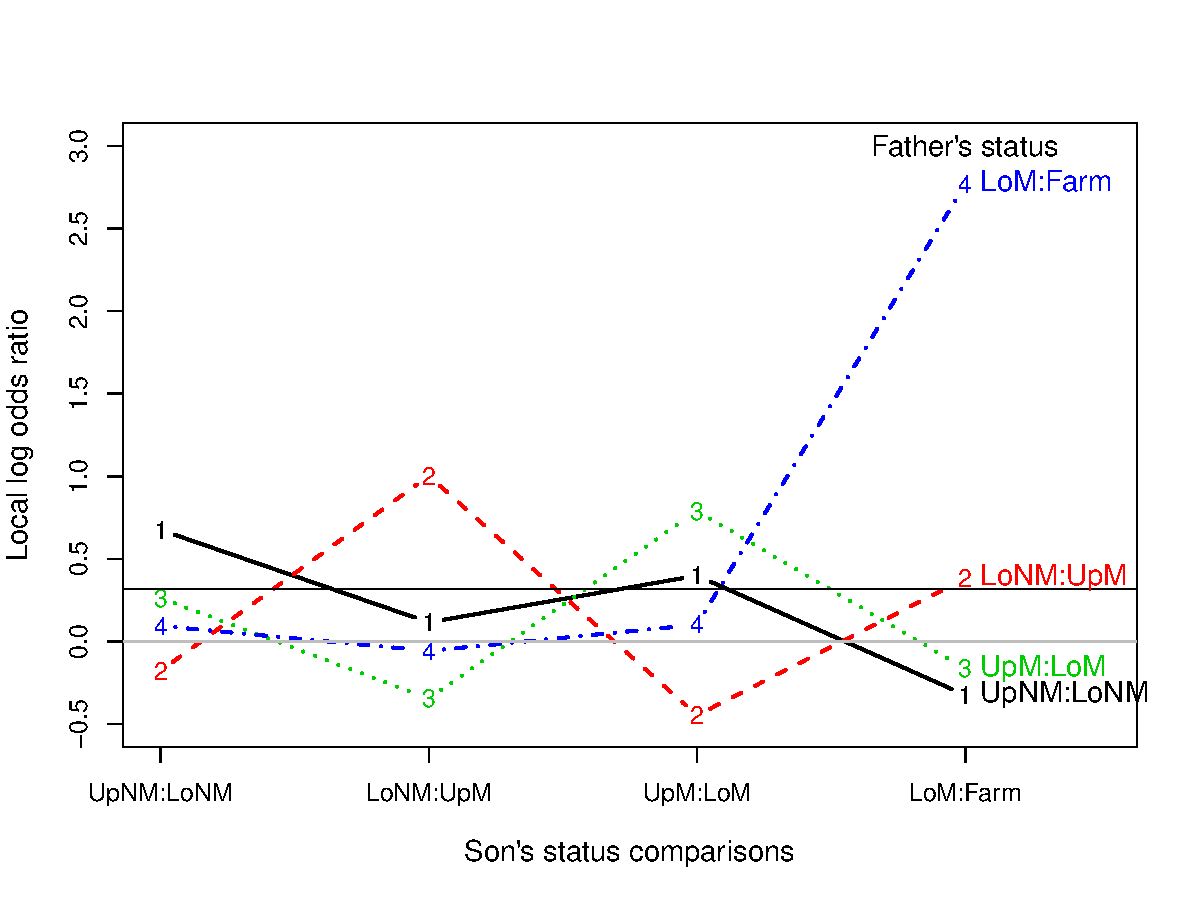
\includegraphics[width=.75\textwidth]{ch08/fig/hauser-lor-plot-1} }

\caption[Plot of observed local log odds ratios in the Hauser79 data]{Plot of observed local log odds ratios in the Hauser79 data. The gray horizontal line at zero shows local independence; the black horizontal line shows the mean.\label{fig:hauser-lor-plot}}
\end{figure}


\end{knitrout}
Amonst the features here, you can see that there is a tendency for the odds ratio
contrasting fathers in the non-manual categories (\code{UpNM:LoNM}) to decline
with the adjacent comparisons of their sons' occupations.  As well, the
$2 \times 2$ table for fathers and sons in the \code{LoM:Farm} stands out
as deserving some attention.  These observed features will be smoothed
by fitting models, as described below.  For additional interpretation, you
can always construct similar plots of the log odds ratios using the
\func{fitted} values from any of the models described below.

We begin by fitting the independence model and the quasi-independence model,
where the diagonal parameters in the latter are specified as
\code{Diag(Father,Son)}.
As expected, given the large frequencies in the diagonal cells,
the quasi-independence model is a considerable improvement, but the fit
is still very poor.
\begin{knitrout}
\definecolor{shadecolor}{rgb}{1, 0.961, 0.933}\color{fgcolor}\begin{kframe}
\begin{alltt}
\hlstd{hauser.indep} \hlkwb{<-} \hlkwd{gnm}\hlstd{(Freq} \hlopt{~} \hlstd{Father} \hlopt{+} \hlstd{Son,} \hlkwc{data}\hlstd{=Hauser79,} \hlkwc{family}\hlstd{=poisson)}
\hlstd{hauser.quasi} \hlkwb{<-}  \hlkwd{update}\hlstd{(hauser.indep,} \hlopt{~} \hlstd{.} \hlopt{+} \hlkwd{Diag}\hlstd{(Father,Son))}
\hlstd{vcdExtra::}\hlkwd{Summarise}\hlstd{(hauser.indep, hauser.quasi)}
\end{alltt}
\begin{verbatim}
## Likelihood summary table:
##               AIC  BIC LR Chisq Df Pr(>Chisq)    
## hauser.indep 6391 6402     6170 16     <2e-16 ***
## hauser.quasi  914  931      683 11     <2e-16 ***
## ---
## Signif. codes:  0 '***' 0.001 '**' 0.01 '*' 0.05 '.' 0.1 ' ' 1
\end{verbatim}
\end{kframe}
\end{knitrout}
The pattern of associations can be seen in the mosaic displays for
both models, shown in \figref{fig:hauser-mosaic1}.
\begin{knitrout}
\definecolor{shadecolor}{rgb}{1, 0.961, 0.933}\color{fgcolor}\begin{kframe}
\begin{alltt}
\hlkwd{mosaic}\hlstd{(hauser.indep,} \hlopt{~}\hlstd{Father}\hlopt{+}\hlstd{Son,} \hlkwc{main}\hlstd{=}\hlstr{"Independence model"}\hlstd{,}
       \hlkwc{gp}\hlstd{=shading_Friendly)}
\hlkwd{mosaic}\hlstd{(hauser.quasi,} \hlopt{~}\hlstd{Father}\hlopt{+}\hlstd{Son,} \hlkwc{main}\hlstd{=}\hlstr{"Quasi-independence model"}\hlstd{,}
       \hlkwc{gp}\hlstd{=shading_Friendly)}
\end{alltt}
\end{kframe}\begin{figure}[!htbp]


\centerline{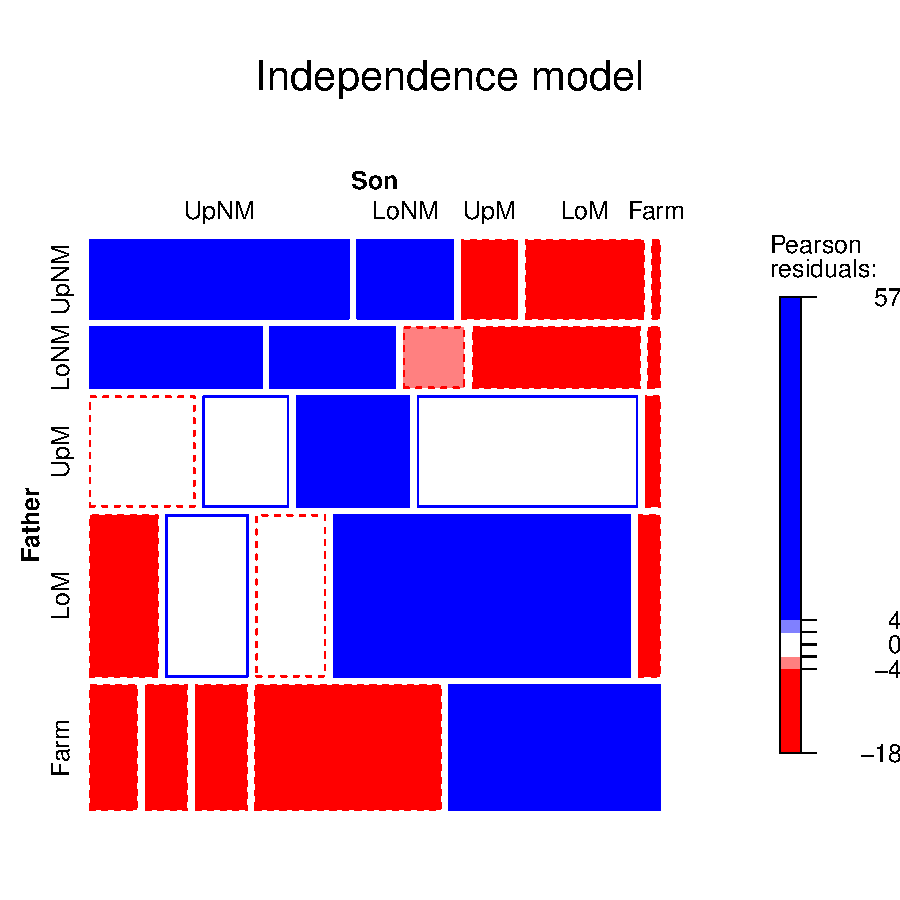
\includegraphics[width=.49\textwidth]{ch08/fig/hauser-mosaic1-1} 
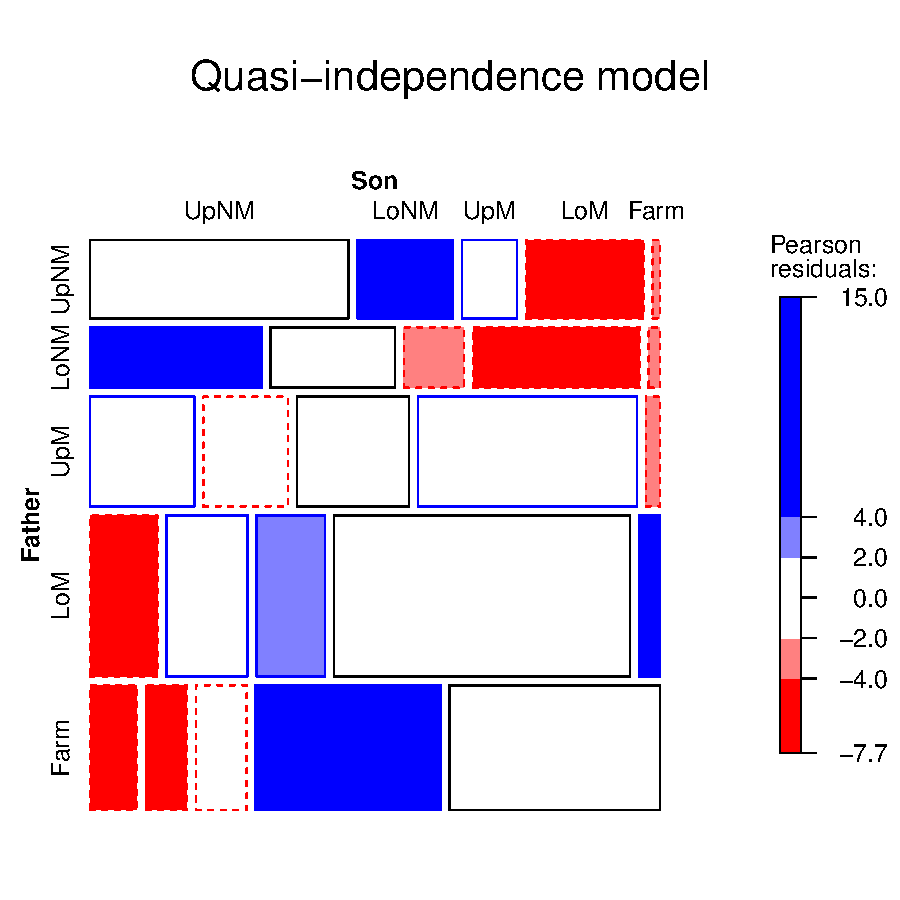
\includegraphics[width=.49\textwidth]{ch08/fig/hauser-mosaic1-2} }

\caption[Mosaic displays for the Hauser79 data]{Mosaic displays for the Hauser79 data. Left: independence model; right:quasi-independence model.\label{fig:hauser-mosaic1}}
\end{figure}


\end{knitrout}

The mosaic for quasi-independence shows an approximately symmetric
pattern of residuals, so we proceed to add \code{Symm(Father,Son)}
to the model to specify quasi-symmetry.
\begin{knitrout}
\definecolor{shadecolor}{rgb}{1, 0.961, 0.933}\color{fgcolor}\begin{kframe}
\begin{alltt}
\hlstd{hauser.qsymm} \hlkwb{<-}  \hlkwd{update}\hlstd{(hauser.indep,}
                        \hlopt{~} \hlstd{.} \hlopt{+} \hlkwd{Diag}\hlstd{(Father,Son)} \hlopt{+} \hlkwd{Symm}\hlstd{(Father,Son))}
\hlstd{vcdExtra::}\hlkwd{Summarise}\hlstd{(hauser.qsymm)}
\end{alltt}
\begin{verbatim}
## Likelihood summary table:
##              AIC BIC LR Chisq Df Pr(>Chisq)    
## hauser.qsymm 268 291     27.4  6    0.00012 ***
## ---
## Signif. codes:  0 '***' 0.001 '**' 0.01 '*' 0.05 '.' 0.1 ' ' 1
\end{verbatim}
\end{kframe}
\end{knitrout}
This model represents a huge improvement in goodness of fit.
With such a large sample size, it might be considered an acceptable
fit. The remaining lack of fit is shown in the
mosaic for this model, \figref{fig:hauser-mosaic2}.
\begin{knitrout}
\definecolor{shadecolor}{rgb}{1, 0.961, 0.933}\color{fgcolor}\begin{kframe}
\begin{alltt}
\hlkwd{mosaic}\hlstd{(hauser.qsymm,} \hlopt{~}\hlstd{Father}\hlopt{+}\hlstd{Son,} \hlkwc{main}\hlstd{=}\hlstr{"Quasi-symmetry model"}\hlstd{,}
       \hlkwc{gp}\hlstd{=shading_Friendly,} \hlkwc{residuals_type}\hlstd{=}\hlstr{"rstandard"}\hlstd{)}
\end{alltt}
\end{kframe}\begin{figure}[!htbp]


\centerline{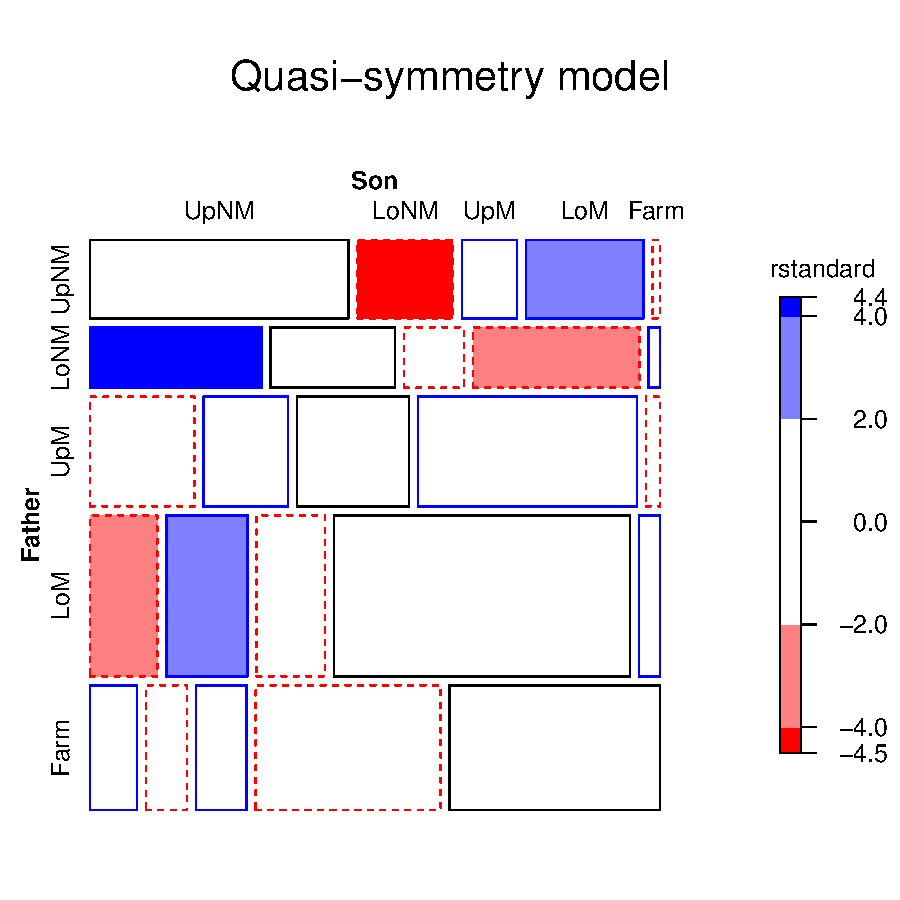
\includegraphics[width=.6\textwidth]{ch08/fig/hauser-mosaic2-1} }

\caption[Mosaic display  for the model of quasi-symmetry fit to the Hauser79 data]{Mosaic display  for the model of quasi-symmetry fit to the Hauser79 data.\label{fig:hauser-mosaic2}}
\end{figure}


\end{knitrout}
The cells with the largest lack of symmetry (using standardized residuals)
are those for the
upper and lower non-manual occupations, where the son of
an upper manual worker is less likely to move to lower non-manual
work than the reverse.

For cases like this involving structured associations in square tables,
\citet{Hauser:79} developed the more general idea of grouping
the row and column categories into levels of an association factor
based on similar values of residuals or local odds ratios observed from
the independence model.  Such models are called \term{topological model}s
or \term{levels model}s, which are implemented in the \func{Topo}.

To illustrate, Hauser suggested the following matrix of levels
to account for the pattern of associations seen in \figref{fig:hauser-mosaic1}.
The coding here takes the diagonal cell for the Farm category as the reference
cell. Four other parameters are assigned by the numbers 2--5 to account for lack
of independence.
\begin{knitrout}
\definecolor{shadecolor}{rgb}{1, 0.961, 0.933}\color{fgcolor}\begin{kframe}
\begin{alltt}
\hlstd{levels} \hlkwb{<-} \hlkwd{matrix}\hlstd{(}\hlkwd{c}\hlstd{(}
  \hlnum{2}\hlstd{,}  \hlnum{4}\hlstd{,}  \hlnum{5}\hlstd{,}  \hlnum{5}\hlstd{,}  \hlnum{5}\hlstd{,}
  \hlnum{3}\hlstd{,}  \hlnum{4}\hlstd{,}  \hlnum{5}\hlstd{,}  \hlnum{5}\hlstd{,}  \hlnum{5}\hlstd{,}
  \hlnum{5}\hlstd{,}  \hlnum{5}\hlstd{,}  \hlnum{5}\hlstd{,}  \hlnum{5}\hlstd{,}  \hlnum{5}\hlstd{,}
  \hlnum{5}\hlstd{,}  \hlnum{5}\hlstd{,}  \hlnum{5}\hlstd{,}  \hlnum{4}\hlstd{,}  \hlnum{4}\hlstd{,}
  \hlnum{5}\hlstd{,}  \hlnum{5}\hlstd{,}  \hlnum{5}\hlstd{,}  \hlnum{4}\hlstd{,}  \hlnum{1}
  \hlstd{),} \hlnum{5}\hlstd{,} \hlnum{5}\hlstd{,} \hlkwc{byrow}\hlstd{=}\hlnum{TRUE}\hlstd{)}
\end{alltt}
\end{kframe}
\end{knitrout}
This models is fit using \func{Topo} as shown below. It also provides a huge
improvement over the independence model, with 4 additional parameters.
\begin{knitrout}
\definecolor{shadecolor}{rgb}{1, 0.961, 0.933}\color{fgcolor}\begin{kframe}
\begin{alltt}
\hlstd{hauser.topo} \hlkwb{<-} \hlkwd{update}\hlstd{(hauser.indep,} \hlopt{~} \hlstd{.} \hlopt{+} \hlkwd{Topo}\hlstd{(Father, Son,} \hlkwc{spec}\hlstd{=levels))}
\hlstd{vcdExtra::}\hlkwd{Summarise}\hlstd{(hauser.topo)}
\end{alltt}
\begin{verbatim}
## Likelihood summary table:
##             AIC BIC LR Chisq Df Pr(>Chisq)    
## hauser.topo 295 311     66.6 12    1.4e-09 ***
## ---
## Signif. codes:  0 '***' 0.001 '**' 0.01 '*' 0.05 '.' 0.1 ' ' 1
\end{verbatim}
\end{kframe}
\end{knitrout}
As with other models fit using \func{gnm}, you can extract the coefficients
for particular terms using \func{pickCoef}.
\begin{knitrout}
\definecolor{shadecolor}{rgb}{1, 0.961, 0.933}\color{fgcolor}\begin{kframe}
\begin{alltt}
\hlkwd{as.vector}\hlstd{((}\hlkwd{coef}\hlstd{(hauser.topo)[}\hlkwd{pickCoef}\hlstd{(hauser.topo,} \hlstr{"Topo"}\hlstd{)]))}
\end{alltt}
\begin{verbatim}
## [1] -1.8128 -2.4973 -2.8035 -3.4026
\end{verbatim}
\end{kframe}
\end{knitrout}

The models fit in this example are summarized below.
Note that AIC prefers the quasi-symmetry model, \code{hauser.quasi},
while, because of the large sample size, BIC prefers the topological model,
\code{hauser.topo}.
\begin{knitrout}
\definecolor{shadecolor}{rgb}{1, 0.961, 0.933}\color{fgcolor}\begin{kframe}
\begin{alltt}
\hlstd{vcdExtra::}\hlkwd{Summarise}\hlstd{(hauser.indep, hauser.quasi, hauser.qsymm, hauser.topo)}
\end{alltt}
\begin{verbatim}
## Likelihood summary table:
##               AIC  BIC LR Chisq Df Pr(>Chisq)    
## hauser.indep 6391 6402     6170 16    < 2e-16 ***
## hauser.quasi  914  931      683 11    < 2e-16 ***
## hauser.qsymm  268  291       27  6    0.00012 ***
## hauser.topo   295  311       67 12    1.4e-09 ***
## ---
## Signif. codes:  0 '***' 0.001 '**' 0.01 '*' 0.05 '.' 0.1 ' ' 1
\end{verbatim}
\end{kframe}
\end{knitrout}


\end{Example}

\subsection{Ordinal square tables}\label{sec:sq-ordinal}
The theory presented in \secref{sec:sq-quasi} treats the row and column variables
as nominal.  In many instances, such as \exref{ex:hauser1},
the variable categories are also ordered, yet these models do not exploit
their ordinal nature.
In such cases, the models such as uniform association ($L \times L$),
row effects, RC and others discussed in \secref{sec:loglin-ordinal}
can be combined with terms for quasi-independence and symmetry of
the remaining associations.

% For example, using ordered, assigned scores
% $\vec{\alpha} = \{ \alpha_i \}$ such that $\alpha_1 \le \alpha_2 \le \cdots \alpha_I$
% for both row and column variables,
% the \term{ordinal quasi-symmetry} model is
% \begin{equation}\label{eq:oquasi-symm}
%  \log m_{ij} = \lambda_i^A + \lambda_j^B + \gamma \alpha_j \lambda_{ij}
%  \comma
% \end{equation}
% where $\lambda_{ij} = \lambda_{ji}$ for $i \ne j$.

For example, the $L \times L$ model \eqref{eq:linlin} of uniform association
applies directly to square tables, and, for square tables, can also be
amended to include a diagonals term, \func{Diag}, giving a model
of \emph{quasi-uniform association}.  In this model, all adjacent
$2 \times 2$ sub-tables not involving diagonal cells have a common
local odds ratio.

A related model is the \term{crossings model} \citep{Goodman:1972}.
This hypothesizes that there are different difficulty parameters
for crossing from one category to the next, and that the associations
between categories decreases with their separation.
In the crossings model for an $I \times I$ table, there
are $I-1$ crossings parameters, $\nu_1, \nu_2, \dots, \nu_{I-1}$.
The association parameters, $\lambda_{ij}^{AB}$ have the form
of the product of the intervening $\nu$ parameters,
% \begin{eqnarray*}
% \lambda_{ij}^{AB} & = & \prod_{k=j}^{k=i-1} \nu_k \quad \mbox{for } i>j \\
%                   & = & \prod_{k=i}^{k=j-1} \nu_k \quad \mbox{for } i<j
% \end{eqnarray*}
\begin{equation*}
\lambda_{ij}^{AB} = \left\{
\begin{array}{r@{\quad : \quad}l}
 \displaystyle \prod_{k=j}^{k=i-1} \nu_k & i>j \\
 \displaystyle \prod_{k=i}^{k=j-1} \nu_k & i<j
\end{array}
\right.
\end{equation*}
This model can also be cast in \emph{quasi} form, by addition of a
\code{Diag} term to fit the main diagonal cells.
See \citet[\S 4.4.7]{PowersXie:2008} for further details of this model.
The \func{Crossings} function in \pkg{vcdExtra} implements such crossings terms.



\begin{Example}[hauser2]{Hauser's occupational mobility table}

Without much comment or detail, for reference
we first fit some of the ordinal models
to the \data{Hauser79} data: Uniform association ($L \times L$), row effects,
and the RC(1) model.

\begin{knitrout}
\definecolor{shadecolor}{rgb}{1, 0.961, 0.933}\color{fgcolor}\begin{kframe}
\begin{alltt}
\hlstd{Fscore} \hlkwb{<-} \hlkwd{as.numeric}\hlstd{(Hauser79}\hlopt{$}\hlstd{Father)}   \hlcom{# numeric scores}
\hlstd{Sscore} \hlkwb{<-} \hlkwd{as.numeric}\hlstd{(Hauser79}\hlopt{$}\hlstd{Son)}      \hlcom{# numeric scores}

\hlcom{# uniform association}
\hlstd{hauser.UA} \hlkwb{<-} \hlkwd{update}\hlstd{(hauser.indep,} \hlopt{~} \hlstd{.} \hlopt{+} \hlstd{Fscore}\hlopt{*}\hlstd{Sscore)}
\hlcom{# row effects model}
\hlstd{hauser.roweff} \hlkwb{<-} \hlkwd{update}\hlstd{(hauser.indep,} \hlopt{~} \hlstd{.} \hlopt{+} \hlstd{Father}\hlopt{*}\hlstd{Sscore)}
\hlcom{# RC model}
\hlstd{hauser.RC} \hlkwb{<-} \hlkwd{update}\hlstd{(hauser.indep,} \hlopt{~} \hlstd{.} \hlopt{+} \hlkwd{Mult}\hlstd{(Father, Son),} \hlkwc{verbose}\hlstd{=}\hlnum{FALSE}\hlstd{)}
\end{alltt}
\end{kframe}
\end{knitrout}
All of these fit very poorly, yet they are all substantial improvements over
the independence model.
\begin{knitrout}
\definecolor{shadecolor}{rgb}{1, 0.961, 0.933}\color{fgcolor}\begin{kframe}
\begin{alltt}
\hlstd{vcdExtra::}\hlkwd{Summarise}\hlstd{(hauser.indep, hauser.UA, hauser.roweff, hauser.RC)}
\end{alltt}
\begin{verbatim}
## Likelihood summary table:
##                AIC  BIC LR Chisq Df Pr(>Chisq)    
## hauser.indep  6391 6402     6170 16     <2e-16 ***
## hauser.UA     2503 2516     2281 15     <2e-16 ***
## hauser.roweff 2309 2325     2080 12     <2e-16 ***
## hauser.RC      920  940      685  9     <2e-16 ***
## ---
## Signif. codes:  0 '***' 0.001 '**' 0.01 '*' 0.05 '.' 0.1 ' ' 1
\end{verbatim}
\end{kframe}
\end{knitrout}

The $L \times L$ model, \code{hauser.UA} might be improved by ignoring the
diagonals, and, indeed it is.
\begin{knitrout}
\definecolor{shadecolor}{rgb}{1, 0.961, 0.933}\color{fgcolor}\begin{kframe}
\begin{alltt}
\hlstd{hauser.UAdiag} \hlkwb{<-} \hlkwd{update}\hlstd{(hauser.UA,} \hlopt{~} \hlstd{.} \hlopt{+} \hlkwd{Diag}\hlstd{(Father,Son))}
\hlkwd{anova}\hlstd{(hauser.UA, hauser.UAdiag,} \hlkwc{test}\hlstd{=}\hlstr{"Chisq"}\hlstd{)}
\end{alltt}
\begin{verbatim}
## Analysis of Deviance Table
## 
## Model 1: Freq ~ Father + Son + Fscore + Sscore + Fscore:Sscore
## Model 2: Freq ~ Father + Son + Fscore + Sscore + Fscore:Sscore + Diag(Father, 
##     Son)
##   Resid. Df Resid. Dev Df Deviance Pr(>Chi)    
## 1        15       2281                         
## 2        10         73  5     2208   <2e-16 ***
## ---
## Signif. codes:  0 '***' 0.001 '**' 0.01 '*' 0.05 '.' 0.1 ' ' 1
\end{verbatim}
\end{kframe}
\end{knitrout}
In this model, the estimated common local log odds ratio---
the coefficient for the linear-by-linear term
\code{Fscore:Sscore} is
\begin{knitrout}
\definecolor{shadecolor}{rgb}{1, 0.961, 0.933}\color{fgcolor}\begin{kframe}
\begin{alltt}
\hlkwd{coef}\hlstd{(hauser.UAdiag)[[}\hlstr{"Fscore:Sscore"}\hlstd{]]}
\end{alltt}
\begin{verbatim}
## [1] 0.1584
\end{verbatim}
\end{kframe}
\end{knitrout}
\noindent For comparisons not involving the diagonal cells,
each step down the scale of occupational categories for the father
multiplies the odds that the son will also be in one lower
category by $\exp (0.158) = 1.172$, an increase of 17\%.

The crossings model, with and without the diagonal cells can be fit as follows:
\begin{knitrout}
\definecolor{shadecolor}{rgb}{1, 0.961, 0.933}\color{fgcolor}\begin{kframe}
\begin{alltt}
\hlstd{hauser.CR} \hlkwb{<-} \hlkwd{update}\hlstd{(hauser.indep,} \hlopt{~} \hlstd{.} \hlopt{+} \hlkwd{Crossings}\hlstd{(Father,Son))}
\hlstd{hauser.CRdiag} \hlkwb{<-} \hlkwd{update}\hlstd{(hauser.CR,} \hlopt{~} \hlstd{.} \hlopt{+} \hlkwd{Diag}\hlstd{(Father,Son))}
\hlstd{vcdExtra::}\hlkwd{Summarise}\hlstd{(hauser.CR, hauser.CRdiag)}
\end{alltt}
\begin{verbatim}
## Likelihood summary table:
##               AIC BIC LR Chisq Df Pr(>Chisq)    
## hauser.CR     319 334     89.9 12    5.1e-14 ***
## hauser.CRdiag 299 318     64.2  9    2.0e-10 ***
## ---
## Signif. codes:  0 '***' 0.001 '**' 0.01 '*' 0.05 '.' 0.1 ' ' 1
\end{verbatim}
\end{kframe}
\end{knitrout}
The quasi-crossings model \code{hauser.CRdiag} has a reasonable \GSQ fit statistic,
and its interpretation and lack of fit is worth exploring further.
The crossings coefficients $\vec{\nu}$ can be extracted as follows.
\begin{knitrout}
\definecolor{shadecolor}{rgb}{1, 0.961, 0.933}\color{fgcolor}\begin{kframe}
\begin{alltt}
\hlstd{nu} \hlkwb{<-} \hlkwd{coef}\hlstd{(hauser.CRdiag)[}\hlkwd{pickCoef}\hlstd{(hauser.CRdiag,} \hlstr{"Crossings"}\hlstd{)]}
\hlkwd{names}\hlstd{(nu)} \hlkwb{<-} \hlkwd{gsub}\hlstd{(}\hlstr{"Crossings(Father, Son)C"}\hlstd{,} \hlstr{"nu"}\hlstd{,} \hlkwd{names}\hlstd{(nu),} \hlkwc{fixed}\hlstd{=}\hlnum{TRUE}\hlstd{)}
\hlstd{nu}
\end{alltt}
\begin{verbatim}
##      nu1      nu2      nu3      nu4 
## -0.42275 -0.38768 -0.27500 -1.40244
\end{verbatim}
\end{kframe}
\end{knitrout}
\noindent They indicate the steps between adjacent categories
in terms of the barriers for a son moving to a lower
occupational category.  The numerically largest gap separates
the lower non-manual category from farming.

In contrast to the \code{UAdiag} model, the quasi-crossing model with
diagonal terms implies that all $2 \times 2$ off-diagonal sub-tables
are independent, i.e., the local odds ratios are all equal to 1.0.
The reasons for lack of fit of this model can be seen in the
corresponding mosaic display, shown in \figref{fig:hauser-mosaic3}

\begin{knitrout}
\definecolor{shadecolor}{rgb}{1, 0.961, 0.933}\color{fgcolor}\begin{kframe}
\begin{alltt}
\hlkwd{mosaic}\hlstd{(hauser.CRdiag,} \hlopt{~}\hlstd{Father}\hlopt{+}\hlstd{Son,}
       \hlkwc{gp}\hlstd{=shading_Friendly,} \hlkwc{residuals_type}\hlstd{=}\hlstr{"rstandard"}\hlstd{,}
       \hlkwc{main}\hlstd{=}\hlstr{"Crossings() + Diag()"}\hlstd{)}
\end{alltt}
\end{kframe}\begin{figure}[!htbp]


\centerline{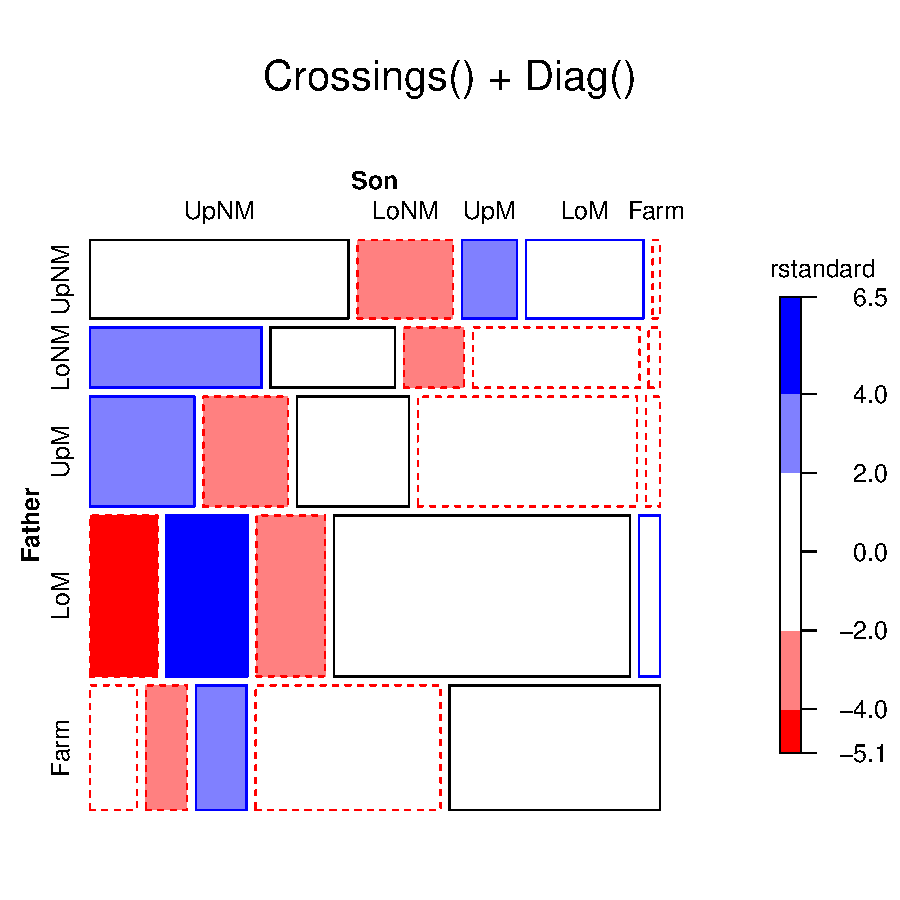
\includegraphics[width=.6\textwidth]{ch08/fig/hauser-mosaic3-1} }

\caption[Mosaic display  for the quasi-crossings model fit to the Hauser79 data]{Mosaic display  for the quasi-crossings model fit to the Hauser79 data.\label{fig:hauser-mosaic3}}
\end{figure}


\end{knitrout}
\noindent It can be seen that lack of fit for this model is largely concentrated in
the lower triangle, where the father's occupation is lower than that of his son.

In this example and the last, we have fit quite a few different models to the
\citet{Hauser:79} data.  In presentations, articles and books it is common to
summarize such a collection in a table, sorted by \GSQ, degrees of freedom,
AIC or BIC, to show their ordering along some metric.
For instance, here we collect all the models fit in \exref{ex:hauser1} and this
example in a \func{glmlist} and sort in decreasing order of BIC
to show model fit by this measure. 
%\DONE{FIXME: won't work with Summarise()}
% <<hauser-sumry>>=
% modlist <- glmlist(hauser.indep, hauser.roweff, hauser.UA, hauser.UAdiag,
%                    hauser.quasi, hauser.qsymm,  hauser.topo,
%                    hauser.RC, hauser.CR, hauser.CRdiag)
% vcdExtra::summarise(modlist, sortby="AIC")
% @

\begin{knitrout}
\definecolor{shadecolor}{rgb}{1, 0.961, 0.933}\color{fgcolor}\begin{kframe}
\begin{alltt}
\hlstd{modlist} \hlkwb{<-} \hlkwd{glmlist}\hlstd{(hauser.indep, hauser.roweff, hauser.UA, hauser.UAdiag,}
                   \hlstd{hauser.quasi, hauser.qsymm,  hauser.topo,}
                   \hlstd{hauser.RC, hauser.CR, hauser.CRdiag)}
\hlkwd{Summarise}\hlstd{(modlist,} \hlkwc{sortby}\hlstd{=}\hlstr{"BIC"}\hlstd{)}
\end{alltt}
\begin{verbatim}
## Likelihood summary table:
##                AIC  BIC LR Chisq Df Pr(>Chisq)    
## hauser.indep  6391 6402     6170 16    < 2e-16 ***
## hauser.UA     2503 2516     2281 15    < 2e-16 ***
## hauser.roweff 2309 2325     2080 12    < 2e-16 ***
## hauser.RC      920  940      685  9    < 2e-16 ***
## hauser.quasi   914  931      683 11    < 2e-16 ***
## hauser.CR      319  334       90 12    5.1e-14 ***
## hauser.UAdiag  306  324       73 10    1.2e-11 ***
## hauser.CRdiag  299  318       64  9    2.0e-10 ***
## hauser.topo    295  311       67 12    1.4e-09 ***
## hauser.qsymm   268  291       27  6    0.00012 ***
## ---
## Signif. codes:  0 '***' 0.001 '**' 0.01 '*' 0.05 '.' 0.1 ' ' 1
\end{verbatim}
\end{kframe}
\end{knitrout}

When there are more than just a few models,
a more useful display is a \term{model comparison plot}
of measures like $\GSQ/df$, AIC or BIC against
degrees of freedom.  For example, \figref{fig:hauser-sumry-plot}
plots \code{BIC} against \code{Df} from the result of \func{Summarise}.
Because interest is focused on the smallest values of BIC
and these values span a large range,
BIC is shown on the log scale using \code{log="y"}.

\begin{knitrout}
\definecolor{shadecolor}{rgb}{1, 0.961, 0.933}\color{fgcolor}\begin{kframe}
\begin{alltt}
\hlstd{sumry} \hlkwb{<-} \hlkwd{Summarise}\hlstd{(modlist)}
\hlstd{mods} \hlkwb{<-} \hlkwd{substring}\hlstd{(}\hlkwd{rownames}\hlstd{(sumry),}\hlnum{8}\hlstd{)}
\hlkwd{with}\hlstd{(sumry, \{}
  \hlkwd{plot}\hlstd{(Df, BIC,} \hlkwc{cex}\hlstd{=}\hlnum{1.3}\hlstd{,} \hlkwc{pch}\hlstd{=}\hlnum{19}\hlstd{,}
       \hlkwc{xlab}\hlstd{=}\hlstr{'Degrees of freedom'}\hlstd{,} \hlkwc{ylab}\hlstd{=}\hlstr{'BIC (log scale)'}\hlstd{,}
       \hlkwc{log}\hlstd{=}\hlstr{"y"}\hlstd{,} \hlkwc{cex.lab}\hlstd{=}\hlnum{1.2}\hlstd{)}
  \hlstd{pos} \hlkwb{<-} \hlkwd{ifelse}\hlstd{(mods}\hlopt{==}\hlstr{"UAdiag"}\hlstd{,} \hlnum{1}\hlstd{,} \hlnum{3}\hlstd{)}
  \hlkwd{text}\hlstd{(Df, BIC}\hlopt{+}\hlnum{55}\hlstd{, mods,} \hlkwc{pos}\hlstd{=pos,} \hlkwc{col}\hlstd{=}\hlstr{'red'}\hlstd{,} \hlkwc{xpd}\hlstd{=}\hlnum{TRUE}\hlstd{, ,} \hlkwc{cex}\hlstd{=}\hlnum{1.2}\hlstd{)}
  \hlstd{\})}
\end{alltt}
\end{kframe}\begin{figure}[!htbp]


\centerline{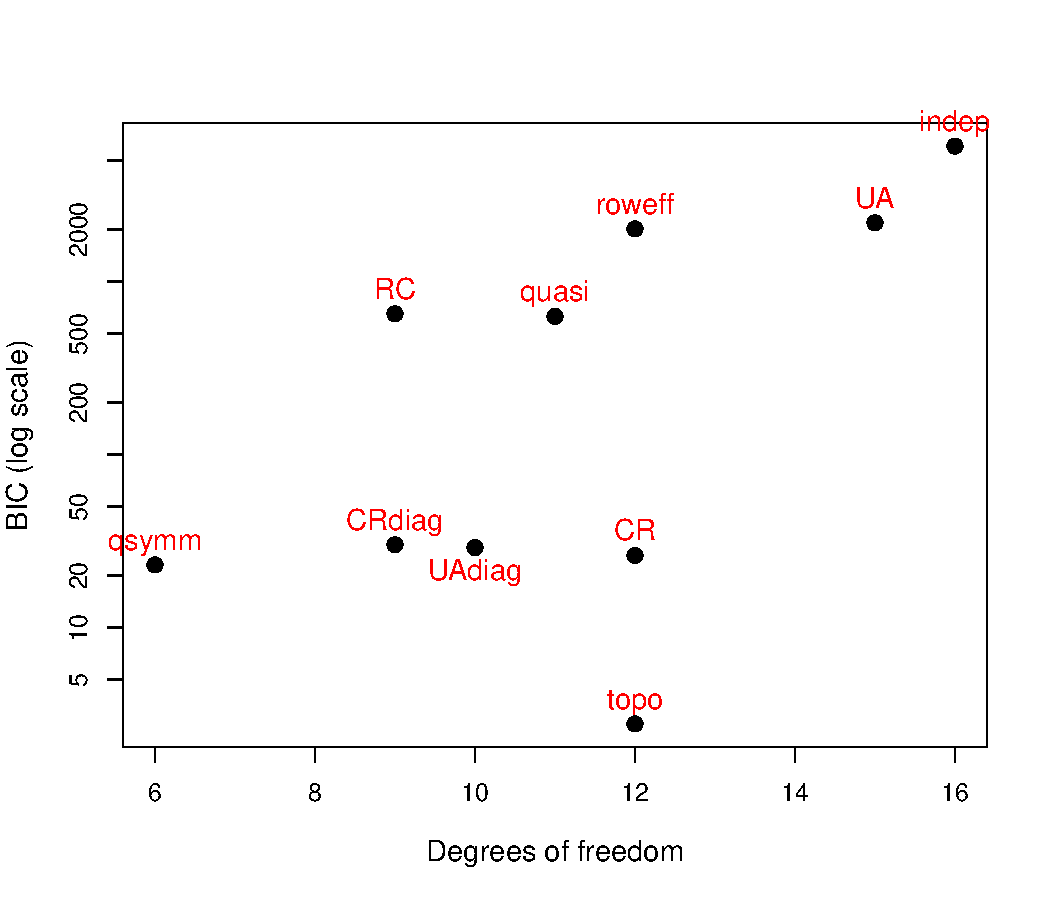
\includegraphics[width=.7\textwidth]{ch08/fig/hauser-sumry-plot-1} }

\caption[Model comparison plot for the models fit to the Hauser79 data]{Model comparison plot for the models fit to the Hauser79 data\label{fig:hauser-sumry-plot}}
\end{figure}


\end{knitrout}
Compared with the sorted tabular display shown above, such a plot sorts the models \emph{both}
by a measure of fit and by model complexity (degrees of freedom).
\figref{fig:hauser-sumry-plot} shows that the quasi-symmetry model is best by BIC,
but also shows that the next four best models by this measure are quite similar
in terms of BIC.  Similar plots for AIC and $\GSQ/df$ show that the model of
quasi-symmetry is favored by these measures.

\end{Example}

\section{Three-way and higher-dimensional tables}\label{sec:loglin-3wayord}

The models and methods for ordinal factors and square tables described in
\secref{sec:loglin-ordinal} and \secref{sec:loglin-square} extend readily
to multidimensional tables with these properties for some of the factors.
In three-way tables, these models provide a more parsimonious account
than the saturated model, $\LLM{ABC}$, and also allow simpler models
than the general model of homogeneous association, $\LLM{AB,AC,BC}$ using
scores for ordinal factors or terms for symmetry and diagonal factors
in square layers.

For example, consider the case where all three factors are ordinal and
the model of homogeneous association $\LLM{AB,AC,BC}$ fits poorly.
In this case we can generalize the model of uniform association by
assigning scores $\vec{a}$, $\vec{b}$ and $\vec{c}$
and model the three-way association,
$\lambda_{ijk}^{ABC}$ as
\begin{equation*}
\lambda_{ijk}^{ABC} = \gamma a_i b_j c_k
\end{equation*}
with only one more parameter. This gives the model of
\term{uniform interaction} (or \emph {homogeneous uniform association})
\begin{equation} \label{eq:uni-inter}
  \log  (m_{ijk})  =
  \mu  +  \lambda_i^A
  +  \lambda_j^B
  +  \lambda_k^C
  +  \lambda_{ij}^{AB}
  +  \lambda_{ik}^{AC}
  +  \lambda_{jk}^{BC}
  +  \gamma a_i b_j c_k
  \period
\end{equation}
This model posits that (with equally spaced scores) all local odds ratios
$\theta_{ijk}$ in adjacent rows, columns and layers are constant,
\begin{equation*}
\log (\theta_{ijk}) = \gamma  \quad\quad \forall \quad i, j, k
\end{equation*}
The homogeneous association model is the special case of $\log \theta_{ijk} = \gamma = 0$.

A less restricted model of \term{heterogeneous uniform association}
retains the linear-by-linear form of association for
factors $A$ and $B$, but allows the strength of this association to vary over
layers, $C$, representing
$\lambda_{ijk}^{ABC}$ as
\begin{equation*}
\lambda_{ijk}^{ABC} = (\gamma + \gamma_k) a_i b_j
\end{equation*}
with the constraint $\sum_k \gamma_k =0$.  This model is equivalent to fitting
separate models of uniform association at each level $k$ of factor $C$
and gives estimates of the conditional local log odds ratios,
$\log \theta_{ij(k)} = \gamma + \gamma_k$.

Following the development in \secref{sec:loglin-ordinal} there is a large
class of other models for ordinal factors (see \figref{fig:assoc-models}),
where not all factors are assigned scores.
For three-way tables, these can be represented in homogeneous form
when the two-way association of $A$ and $B$ is the same for all levels
of $C$, or in a heterogeneous form, when it varies over $C$.

Similarly, the models for square tables described in \secref{sec:loglin-square}
extend to three-way tables with several layers (strata), allowing both homogeneous and
heterogeneous terms for diagonals and symmetry
describing the $AB$ association over levels of $C$.

\begin{Example}[vision-glm2]{Visual acuity}
We continue the analysis of the \data{VisualAcuity} data,
but now consider the three-way, $4 \times 4\times 2$
table comprising both men and women.  The main questions
here are whether the pattern of quasi-symmetry observed in the
analysis for women also pertains to men and whether there
is heterogeneity of the association between right, left acuity
across gender.

A useful first step for $n$-dimensional tables is to consider
the models composed of all 1-way, 2-way, $\dots n$-way terms
as a quick overview.  The function \func{Kway} in \Rpackage{vcdExtra}
does this automatically, returning a \class{glmlist} object
containing the fitted models.%
\footnote{
For completeness, this also fits the 0-way model, corresponding to
$\log m_{ijk\dots} = \mu$, or the model formula \code{Freq} $\sim$ \code{1}.
}

\begin{knitrout}
\definecolor{shadecolor}{rgb}{1, 0.961, 0.933}\color{fgcolor}\begin{kframe}
\begin{alltt}
\hlstd{vis.kway} \hlkwb{<-}\hlkwd{Kway}\hlstd{(Freq} \hlopt{~} \hlstd{right} \hlopt{+} \hlstd{left} \hlopt{+} \hlstd{gender,} \hlkwc{data}\hlstd{=VisualAcuity)}
\hlstd{vcdExtra::}\hlkwd{Summarise}\hlstd{(vis.kway)}
\end{alltt}
\begin{verbatim}
## Likelihood summary table:
##          AIC   BIC LR Chisq Df Pr(>Chisq)    
## kway.0 13857 13858    13631 31    < 2e-16 ***
## kway.1  9925  9937     9686 24    < 2e-16 ***
## kway.2   298   332       28  9    0.00079 ***
## kway.3   287   334        0  0    < 2e-16 ***
## ---
## Signif. codes:  0 '***' 0.001 '**' 0.01 '*' 0.05 '.' 0.1 ' ' 1
\end{verbatim}
\end{kframe}
\end{knitrout}
This shows that the model of homogeneous association \code{kway.2}
($\LLM{RL, RG, LG}$) does not fit well, but it doesn't account
for diagonal agreement or symmetry to simplify the associations.

As a basis for comparison, we first fit the simple models of
quasi-independence and quasi-symmetry that do not involve \var{gender},
asserting the same pattern of diagonal and off-diagonal cells for males
and females.
\begin{knitrout}
\definecolor{shadecolor}{rgb}{1, 0.961, 0.933}\color{fgcolor}\begin{kframe}
\begin{alltt}
\hlstd{vis.indep} \hlkwb{<-} \hlkwd{glm}\hlstd{(Freq} \hlopt{~} \hlstd{right} \hlopt{+} \hlstd{left} \hlopt{+} \hlstd{gender,}  \hlkwc{data} \hlstd{= VisualAcuity,}
                 \hlkwc{family}\hlstd{=poisson)}
\hlstd{vis.quasi} \hlkwb{<-} \hlkwd{update}\hlstd{(vis.indep, .} \hlopt{~} \hlstd{.} \hlopt{+} \hlkwd{Diag}\hlstd{(right, left))}
\hlstd{vis.qsymm} \hlkwb{<-} \hlkwd{update}\hlstd{(vis.indep, .} \hlopt{~} \hlstd{.} \hlopt{+} \hlkwd{Diag}\hlstd{(right, left)} \hlopt{+} \hlkwd{Symm}\hlstd{(right, left))}

\hlkwd{Summarise}\hlstd{(vis.indep, vis.quasi, vis.qsymm)}
\end{alltt}
\begin{verbatim}
## Likelihood summary table:
##            AIC  BIC LR Chisq Df Pr(>Chisq)    
## vis.indep 9925 9937     9686 24     <2e-16 ***
## vis.quasi  696  714      449 20     <2e-16 ***
## vis.qsymm  435  456      184 18     <2e-16 ***
## ---
## Signif. codes:  0 '***' 0.001 '**' 0.01 '*' 0.05 '.' 0.1 ' ' 1
\end{verbatim}
\end{kframe}
\end{knitrout}
The model of homogeneous quasi-symmetry fits quite badly, even worse than the all two-way
association model.  We can see why in the mosaic for this model, shown in \figref{fig:vision2-qsymm}.
\begin{knitrout}
\definecolor{shadecolor}{rgb}{1, 0.961, 0.933}\color{fgcolor}\begin{kframe}
\begin{alltt}
\hlkwd{mosaic}\hlstd{(vis.qsymm,} \hlopt{~} \hlstd{gender} \hlopt{+} \hlstd{right} \hlopt{+} \hlstd{left,} \hlkwc{condvars}\hlstd{=}\hlstr{"gender"}\hlstd{,}
       \hlkwc{residuals_type}\hlstd{=}\hlstr{"rstandard"}\hlstd{,} \hlkwc{gp}\hlstd{=shading_Friendly,}
       \hlkwc{labeling_args}\hlstd{=largs,}
       \hlkwc{main}\hlstd{=}\hlstr{"Homogeneous quasi-symmetry"}\hlstd{)}
\end{alltt}
\end{kframe}\begin{figure}[!htbp]


\centerline{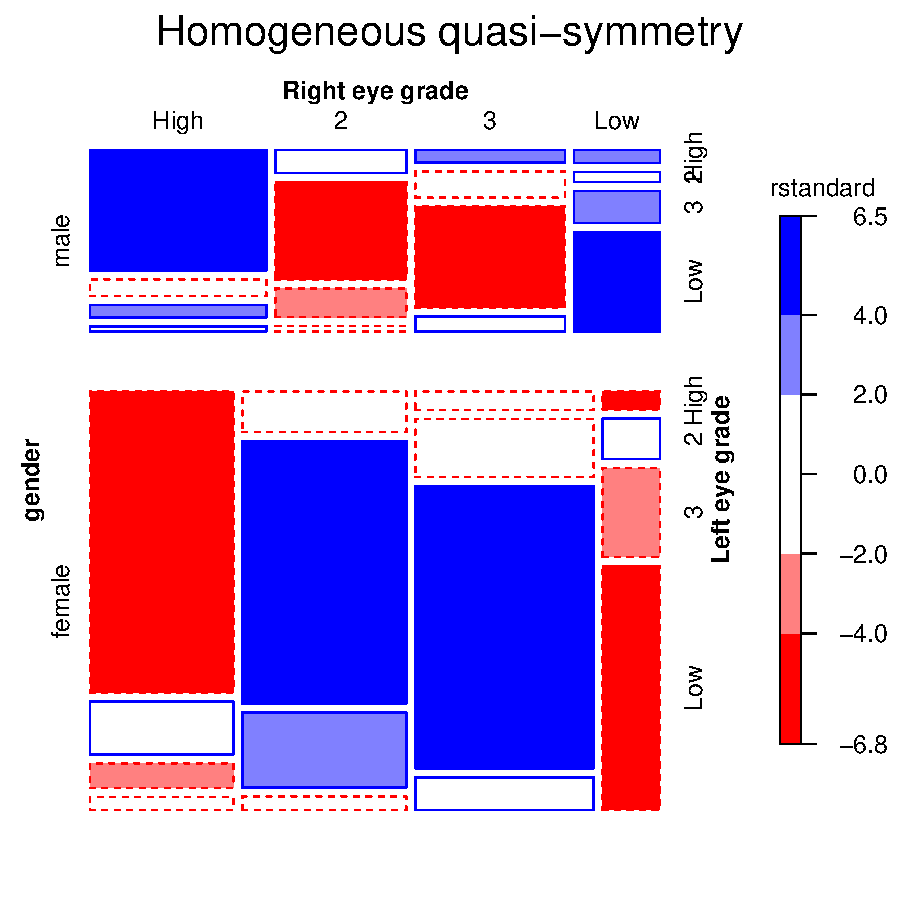
\includegraphics[width=.7\textwidth]{ch08/fig/vision2-qsymm-1} }

\caption[Mosaic display for the model of homogeneous quasi-symmetry fit to the VisualAcuity data]{Mosaic display for the model of homogeneous quasi-symmetry fit to the VisualAcuity data.\label{fig:vision2-qsymm}}
\end{figure}


\end{knitrout}
It can be seen in \figref{fig:vision2-qsymm} that the pattern of residuals for men and women are nearly completely opposite
in the upper and lower portions of the plot: men have positive residuals in the same
\code{right}, \code{left} cells where women have negative residuals, and vice-versa.
In particular, the diagonal cells of both tables have large absolute residuals, because
the term \code{Diag(right, left)} fits a common set of diagonals for both men and women.

We can correct for this by allowing separate diagonal and symmetry terms, given
as interactions of \code{gender} with \func{Diag} and \func{Symm}.

\begin{knitrout}
\definecolor{shadecolor}{rgb}{1, 0.961, 0.933}\color{fgcolor}\begin{kframe}
\begin{alltt}
\hlstd{vis.hetdiag} \hlkwb{<-} \hlkwd{update}\hlstd{(vis.indep, .} \hlopt{~} \hlstd{.} \hlopt{+} \hlstd{gender}\hlopt{*}\hlkwd{Diag}\hlstd{(right, left)} \hlopt{+}
                      \hlkwd{Symm}\hlstd{(right, left))}
\hlstd{vis.hetqsymm} \hlkwb{<-} \hlkwd{update}\hlstd{(vis.indep, .} \hlopt{~} \hlstd{.} \hlopt{+} \hlstd{gender}\hlopt{*}\hlkwd{Diag}\hlstd{(right, left)} \hlopt{+}
                       \hlstd{gender}\hlopt{*}\hlkwd{Symm}\hlstd{(right, left))}
\hlcom{#vis.hetmodels <- glmlist(vis.qsymm, vis.hetdiag, vis.hetqsymm)}
\hlkwd{Summarise}\hlstd{(vis.qsymm, vis.hetdiag, vis.hetqsymm)}
\end{alltt}
\begin{verbatim}
## Likelihood summary table:
##              AIC BIC LR Chisq Df Pr(>Chisq)    
## vis.qsymm    435 456    183.7 18    < 2e-16 ***
## vis.hetdiag  312 338     52.3 14    2.5e-06 ***
## vis.hetqsymm 287 321     17.7  9      0.038 *  
## ---
## Signif. codes:  0 '***' 0.001 '**' 0.01 '*' 0.05 '.' 0.1 ' ' 1
\end{verbatim}
\end{kframe}
\end{knitrout}
\noindent Note that the model \code{vis.hetqsymm} fits better than the model \code{vis.hetdiag}
in absolute terms and by AIC, but the latter, with fewer parameters, fits better by BIC.
The mosaic for the model \code{vis.hetqsymm} is shown in \figref{fig:vision2-hetqsymm}.
\begin{knitrout}
\definecolor{shadecolor}{rgb}{1, 0.961, 0.933}\color{fgcolor}\begin{kframe}
\begin{alltt}
\hlkwd{mosaic}\hlstd{(vis.hetqsymm,} \hlopt{~} \hlstd{gender} \hlopt{+} \hlstd{right} \hlopt{+} \hlstd{left,} \hlkwc{condvars}\hlstd{=}\hlstr{"gender"}\hlstd{,}
       \hlkwc{residuals_type}\hlstd{=}\hlstr{"rstandard"}\hlstd{,} \hlkwc{gp}\hlstd{=shading_Friendly,}
       \hlkwc{labeling_args}\hlstd{=largs,}
       \hlkwc{main}\hlstd{=}\hlstr{"Heterogeneous quasi-symmetry"}\hlstd{)}
\end{alltt}
\end{kframe}\begin{figure}[!htbp]


\centerline{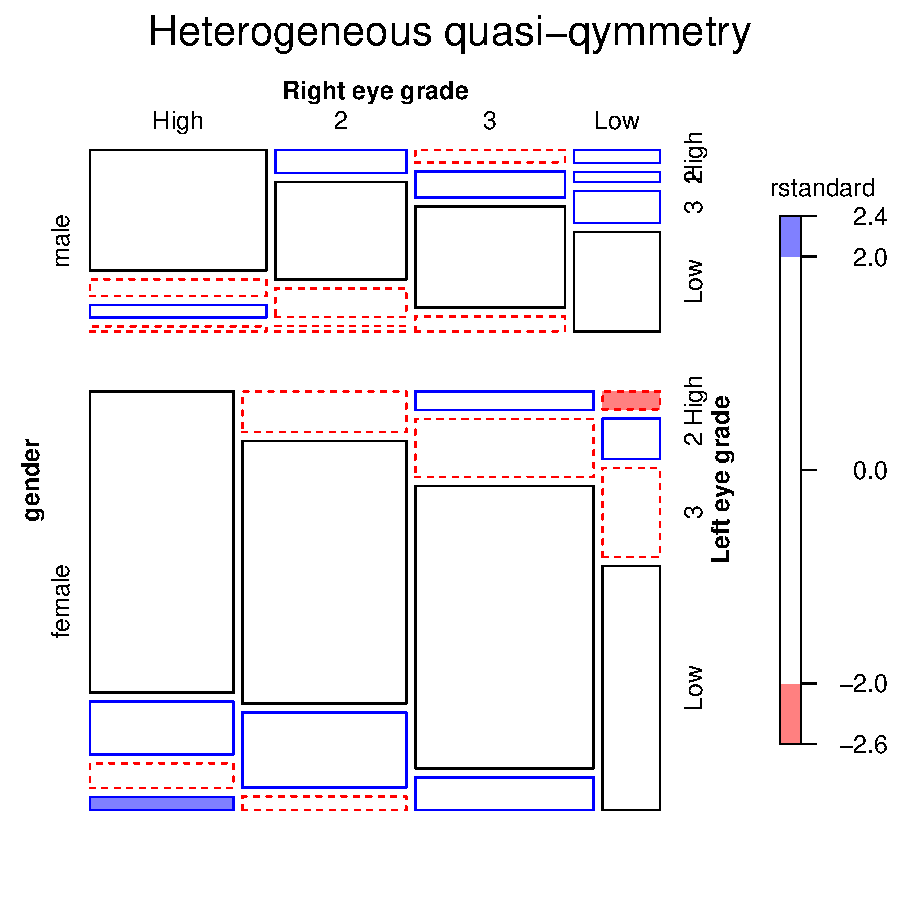
\includegraphics[width=.7\textwidth]{ch08/fig/vision2-hetqsymm-1} }

\caption[Mosaic display for the model of heterogeneous quasi-symmetry fit to the VisualAcuity data]{Mosaic display for the model of heterogeneous quasi-symmetry fit to the VisualAcuity data.\label{fig:vision2-hetqsymm}}
\end{figure}


\end{knitrout}
As in the two-way case, this model now fits the diagonal cells in each table exactly,
effectively ignoring this part of the association between right and left eye
acuity. All remaining residuals are relatively small in magnitude, except for the
two opposite off-diagonal cells \code{(Low, High)} and \code{(High, Low)} in the
table for women.

The substantive interpretation of this example is that
visual acuity is largely the same (diagonal cells)
in the right and left eyes of both men and women.  Ignoring the diagonal cells,
when visual acuity differs, both men and women exhibit approximately symmetric
associations.  However, deviations from symmetry (\figref{fig:vision2-qsymm})
are such that men are slightly more likely to have a lower grade in the right eye,
while women are slightly more likely to have a higher grade in the right eye.


%\TODO{Complete this example with models and plots}

\end{Example}

%\section{An extended example}\label{sec:loglin-vietnam}

%\section{Influence and diagnostic plots for \loglin\ models}\label{sec:loglin-infl}

\section{Multivariate responses}\label{sec:loglin-multiv}


%\section{Multivariate responses}\label{sec:loglin-multiv}

In many studies, there may be \emph{several} categorical responses observed
along with one or more explanatory variables.
In a clinical trial, for example, the efficacy of a drug might be the
primary response, but the occurrence of side-effects might give rise to
additional response variables of substantive interest.
Or, in a study of occupational health, the occurrence of two or more
distinct symptoms might be treated as response variables.

If there are \emph{no} explanatory variables, then the problem is simply to
understand the joint distribution of the response categories,
and the \loglin models and graphical displays described earlier
are sufficient.
Otherwise,
in these cases we usually wish to understand how the various responses
are affected by the explanatory variables.
Moreover, it may also be important to understand how the association
between the categorical responses depends on the explanatory variables.
That is, we would like to study how \emph{both} the marginal distributions
of the responses, and their joint distribution depends on the
predictors.  In the occupational health example, the goal might be
to understand both how the prevalence of several symptoms varies with
one or more predictors, and how the association
(loosely, ``correlation'') among those symptoms varies with those predictors.

Although the general \loglin model is often used in these situations,
there are special reparameterizations that
may be used to separate the \emph{marginal} dependence of each response
on the explanatory variables from the relationship of the
\emph{association} among the responses on the explanatory variables.

Let us say that categorical responses, $Y_1$, $Y_2, \dots$ have been
observed, together with possible explanatory variables,
$X_1$, $X_2, \dots$,
and let $\pi_{ij\cdots}$ be the joint probability of all the responses
and explanatory variables;
we also use
$\vec{x}$ to refer to the values of $X_1$, $X_2, \dots$.

Note that the minimal model of independence of all responses from each other
and from the explanatory variables is the \loglin model
$[Y_1] [Y_2] \cdots [X_1 X_2 \cdots]$
(i.e., all associations among the $X_i$ must be included).
A no-effect model, in which the responses do not depend on the
explanatory variables, but may be associated among themselves is
$[Y_1 Y_2 \cdots] [X_1 X_2 \cdots]$.  However,  these models do not separate
the individual
(marginal) effects of $X_1, X_2 \dots$ on each $Y_i$ from their associative effects
on the joint relationships among the $Y_i$.

There are three useful general approaches which \emph{do} separate these effects:
\begin{enumerate}
\item Model the marginal dependence of each response, $Y_i$ separately on $X_1$, $X_2, \dots$,
and, in addition, model the interdependence among the responses,
$Y_1, Y_2, \dots$.%
\footnote{
For quantitative responses, this is roughly analogous to fitting
univariate response models for each $Y_i$, followed by something like
a principal component analysis of the relationships among the $Y_i$.
But in this case, the multivariate linear model,
$\mat{Y} = \mat{X} \mat{B} + \mat{E}$ provides a general solution.
}
\item Model the joint dependence of all responses on $X_1$, $X_2, \dots$,
but parameterized so that marginal and associative effects are delineated.
\item Construct simultaneous models, estimated together, for the
marginal and joint dependence of the responses on the explanatory variables.
\end{enumerate}

The first approach is the simplest, an informative starting place,
and is satisfactory in the (often unlikely) case that the responses
are not associated, or if the associations among responses do not vary much
over the explanatory variables (i.e., no terms like $[Y_1 Y_2 X_j]$ are
required).  In the clinical trial example, we would construct separate
\loglin or logit models for efficacy of the drug, and for occurrence
of side-effects, and supplement these analyses with mosaic or other
displays showing the relations between efficacy and side-effects
and a model for their joint association. If those who improve
with the drug also show more serious side effects, the worth of the
treatment would be questioned.
A limitation of this method is that it does not provide an overall
model comprising these effects.

In the second approach, the joint probabilities,  $\pi_{ij\cdots}$,
are recast to give separate information regarding the
dependence of the univariate marginal probabilities
$\pi_{i\bullet}, \pi_{\bullet j}, \dots$,
on the explanatory variables
and the dependence of the intra-response associations on
the explanatory variables.
The \Rpackage{VGAM} provides several versions of this approach
with the function \func{vglm} (for \emph{vector generalized linear model}).

The third approach, developed, for example,  by \citet{LangAgresti:94},
is the most general, and provides a scheme to represent
a model $\mathcal{J}(\bullet)$ for the joint distributions of the
$X$, $Y$ variables together with a model $\mathcal{M}(\bullet)$
for their first-order marginal distributions.
The joint models are typically \loglin models, ranging from the
mutual independence model,
$\mathcal{J}(I) = \LLM{Y_1, Y_2, \cdots, X_1, X_2, \cdots}$
to the saturated model,
$\mathcal{J}(S) = \LLM{Y_1 Y_2 \cdots X_1 X_2 \cdots}$,
while the marginal
models are logit models for the response variables.
The combined model, denoted $\mathcal{J}(\bullet) \cap \mathcal{M}(\bullet)$,
is estimated simultaneously by maximum likelihood.
This approach is implemented in \R in the \Rpackage{hmmm}
(hierarchical multinomial marginal models).  However, model specification
in this implementation is complicated, and it will not be considered further
here.

\subsection{Bivariate, binary response models}

We focus here on two related models reflecting the second approach,
as discussed by \citet[Section 6.5]{McCullaghNelder:89}.
We consider here only the case of two binary responses,
though the general approach can be applied to $R>2$ responses
$Y_1, Y_2, \dots , Y_R$, and these may be polytomous or ordinal.

Let $\vec{x}$
refer to the values of all the explanatory variables and let $\pi _{ij}\left(
\vec{x}\right) $ be the joint probabilities in cell $Y_1=i,\,Y_2=j$.
The essential idea of the
\term{bivariate logistic model} arises from a linear transformation of the
cell probabilities $\vec{\pi}$ to interpretable functions of the marginal
probabilities (logits) and their association (odds ratio),
a mapping of $\vec{\pi} \to \vec{\eta}$,
\begin{eqnarray}
\eta_1    & = & \logit (\pi_{1\bullet })                    \nonumber  \\
\eta_2    & = & \logit (\pi_{\bullet 1})                    \label{eq:blogits}  \\
\eta_{12} & = & \frac{\pi_{11} \, \pi_{22}}{\pi_{12} \, \pi_{21}} \nonumber
\end{eqnarray}
The predictors in $\vec{x}$ are then taken into account by considering models
that relate $\vec{\pi}$ to $\vec{x}$ through $\vec{\eta}$,
\begin{eqnarray}
\eta_1    & = & \vec{x}_1 \trans \vec{\beta}_1     \nonumber  \\
\eta_2    & = & \vec{x}_2 \trans \vec{\beta}_2      \label{eq:blogits2} \\
\eta_{12} & = & \vec{x}_{12} \trans \vec{\beta}_{12} \nonumber
\end{eqnarray}
where $\vec{x}_1$, $\vec{x}_2$ and $\vec{x}_{12}$ are subsets of the predictors
in $\vec{x}$ for each sub-model, and $\vec{\beta}_1$, $\vec{\beta}_1$ and
$\vec{\beta}_{12}$ are the corresponding parameters to be estimated.


\citet{McCullaghNelder:89} arrive at this joint bivariate model in two steps.
First, transform the cell probabilities $\vec{\pi}$
to a vector of probabilities $\vec{\gamma}$ which also includes the
univariate margins, given by
\begin{equation}\label{eq:gamma1}
\vec{\gamma} = \mat{L} \vec{\pi}
\end{equation}
where $\mat{L}$ is a matrix of 0s and 1s of the form of a factorial
design matrix. In the $2\times 2$ case,
\begin{equation}\label{eq:gamma2}
\vec{\gamma =}\left(
\begin{array}{c}
\pi _{1\bullet } \\
\pi _{2\bullet } \\
\pi _{\bullet 1} \\
\pi _{\bullet 2} \\
\pi _{11} \\
\pi _{12} \\
\pi _{21} \\
\pi _{22}
\end{array}
\right) =\left[
\begin{array}{cccc}
1 & 1 & 0 & 0 \\
0 & 0 & 1 & 1 \\
1 & 0 & 1 & 0 \\
0 & 1 & 0 & 1 \\
1 & 0 & 0 & 0 \\
0 & 1 & 0 & 0 \\
0 & 0 & 1 & 0 \\
0 & 0 & 0 & 1
\end{array}
\right] \left(
\begin{array}{c}
\pi _{11} \\
\pi _{12} \\
\pi _{21} \\
\pi _{22}
\end{array}
\right) \period
\end{equation}

There are of course only three linearly independent probabilities, because
$\sum \sum \pi _{ij}=1$. In the second step,
the bivariate logistic model is formulated in terms
of factorial contrasts on the elements of $\vec{\gamma }$ which express
separate models for the two logits and the log odds. The model is expressed
as
\begin{equation}\label{eq:eta1}
 \vec{\eta }=\mat{C}\log \vec{\gamma} =\mat{C} \log \mat{L} \vec{\pi}
 \comma
\end{equation}
where $\mat{C}$ is a matrix of contrasts. In the $2\times 2$ case, the
usual contrasts may be defined by
\begin{equation}\label{eq:eta2}
\vec{\eta }=\left(
\begin{array}{c}
\eta _1 \\
\eta _2 \\
\eta _{12}
\end{array}
\right) =\left(
\begin{array}{c}
\mathrm{logit}\;\pi _{1\bullet } \\
\mathrm{logit}\;\pi _{\bullet 1} \\
\theta_{12}
\end{array}
\right) =\left[
\begin{array}{rrrrrrrr}
1 & -1 & 0 & 0 & 0 & 0 & 0 & 0 \\
0 &  0 & 1 & -1 & 0 & 0 & 0 & 0 \\
0 &  0 & 0 & 0 & 1 & -1 & -1 & 1
\end{array}
\right] \left(
\begin{array}{c}
\pi _{1\bullet } \\
\pi _{2\bullet } \\
\pi _{\bullet 1} \\
\pi _{\bullet 2} \\
\pi _{11} \\
\pi _{12} \\
\pi _{21} \\
\pi _{22}
\end{array}
\right)
\end{equation}
Thus,
we are modeling the marginal odds of each response, together
with the log odds ratio $\theta_{12}$ simultaneously.

Specific models are then formulated for the dependence of $\eta _1 (\vec{x})
, \eta _2 (\vec{x}) $ and $\eta _{12}(\vec{x}) $
on some or all of the explanatory variables. For example, with one quantitative
explanatory variable, $x$, the model
\begin{equation}\label{eq:bilogit1}
\left(
\begin{array}{c}
\eta _1 \\
\eta _2 \\
\eta _{12}
\end{array}
\right) =\left(
\begin{array}{c}
\alpha _1+\beta _1 x \\
\alpha _2+\beta _2 x \\
\theta
\end{array}
\right)
\end{equation}
asserts that the log odds of each response changes linearly with $x$, while
the odds ratio between the responses remains constant. In the general form
given by \cite{McCullaghNelder:89} the submodels in \eqref{eq:bilogit1} may
each depend on the explanatory variables in different ways.
For example, the logits could both depend quadratically on $x$,
while an intercept-only model could be posited for the log odds ratio.

The second model is the \term{bivariate loglinear model},
the special case obtained by taking
$\mat{L}=\mat{I}$ in \eqref{eq:gamma1} and \eqref{eq:eta1}
so that $\vec{\gamma} = \vec{\pi}$.
Then a \loglin\ model of the form
\begin{equation*}
\vec{\eta } ( \vec{x} ) = \mat{C} \log \vec{\pi}
\end{equation*}
expresses contrasts among log probabilities as linear functions of
the explanatory variables.  For the $2 \times 2$ case, we take the
contrasts $\mat{C}$ as shown below
\begin{equation}\label{eq:eta3}
 \vec{\eta }=\left(
 \begin{array}{c}
  l_1 \\
  l_2 \\
  \eta _{12}
 \end{array}
 \right) =\left[
 \begin{array}{rrrr}
  1 & 1 & -1 & -1 \\
  1 & -1 & 1 & -1 \\
  1 & -1 & 1 & -1
 \end{array}
\right] \left(
 \begin{array}{c}
  \log \,\pi_{11} \\
  \log \,\pi_{12} \\
  \log \,\pi_{21} \\
  \log \,\pi_{22}
 \end{array}
\right)
\end{equation}
and models for the dependence of
$l_1( \vec{x})$ , $l_2(\vec{x}) $ and $\eta _{12}(\vec{x})$
are expressed in the same way as in \eqref{eq:bilogit1}.
The estimates of the odds ratio, $\eta_{12}$ are the same under both
models.  The marginal functions are parameterized differently, however,
but lead to similar predicted probabilities.

In \R, bivariate logistic models of the form \eqref{eq:blogits} and
\eqref{eq:blogits2} can be fit using \func{vglm} with
the \func{binom2.or} family in the \Rpackage{VGAM}.%
\footnote{
This package also provides for bivariate and trivariate loglinear models
with \func{loglinb2} and \code{loglinb2}.
}
The fitting and graphing of these models is illustrated in the
next example.


\begin{Example}[coalminers]{Breathlessness and wheeze in coal miners}
In \exref{ex:wheeze1} we examined the association between the occurrence
of two pulmonary conditions, breathlessness and wheeze,
among coal miners classified by age \citep{AshfordSowden:70}.
\figref{fig:coalminer1} showed fourfold displays focused on the odds ratio
for the co-occurrence of these symptoms,
and \figref{fig:coalminer3} plotted these odds ratios against age directly.
Here, we consider models which examine the changes in prevalence of
the two symptoms over age, together with the changes in their association.

\subsubsection*{Plotting bivariate response data}
As a starting point and overview of what is necessary for
bivariate response models,
we calculate the empirical log odds for breathlessness and for
wheeze, and the log odds ratio for their association
in each $2 \times 2$ table.
The log odds ratios are the same values plotted in \figref{fig:coalminer3}
(but the youngest age group was not included in the earlier analysis).

The \data{CoalMiners} data is $2 \times 2 \times 9$ table.  For convenience
in this analysis (and for use with \pkg{VGAM})
we convert it to a $4 \times 9$ data frame, and
relabel the columns to use the combinations of
\code{("B", "b")} and \code{("W", "w")} to represent the conditions
of breathlessness and wheeze, where the upper case letter indicates
presence of the condition.  A variable \var{age} is also created,
using the midpoints of the age categories.
\begin{knitrout}
\definecolor{shadecolor}{rgb}{1, 0.961, 0.933}\color{fgcolor}\begin{kframe}
\begin{alltt}
\hlkwd{data}\hlstd{(}\hlstr{"CoalMiners"}\hlstd{,} \hlkwc{package}\hlstd{=}\hlstr{"vcd"}\hlstd{)}
\hlstd{coalminers} \hlkwb{<-} \hlkwd{data.frame}\hlstd{(}\hlkwd{t}\hlstd{(}\hlkwd{matrix}\hlstd{(}\hlkwd{aperm}\hlstd{(CoalMiners,} \hlkwd{c}\hlstd{(}\hlnum{2}\hlstd{,}\hlnum{1}\hlstd{,}\hlnum{3}\hlstd{)),}
                                  \hlnum{4}\hlstd{,} \hlnum{9}\hlstd{)))}
\hlkwd{colnames}\hlstd{(coalminers)} \hlkwb{<-} \hlkwd{c}\hlstd{(}\hlstr{"BW"}\hlstd{,} \hlstr{"Bw"}\hlstd{,} \hlstr{"bW"}\hlstd{,} \hlstr{"bw"}\hlstd{)}
\hlstd{coalminers}\hlopt{$}\hlstd{age} \hlkwb{<-} \hlkwd{c}\hlstd{(}\hlnum{22}\hlstd{,} \hlnum{27}\hlstd{,} \hlnum{32}\hlstd{,} \hlnum{37}\hlstd{,} \hlnum{42}\hlstd{,} \hlnum{47}\hlstd{,} \hlnum{52}\hlstd{,} \hlnum{57}\hlstd{,} \hlnum{62}\hlstd{)}
\hlstd{coalminers}
\end{alltt}
\begin{verbatim}
##    BW  Bw  bW   bw age
## 1   9   7  95 1841  22
## 2  23   9 105 1654  27
## 3  54  19 177 1863  32
## 4 121  48 257 2357  37
## 5 169  54 273 1778  42
## 6 269  88 324 1712  47
## 7 404 117 245 1324  52
## 8 406 152 225  967  57
## 9 372 106 132  526  62
\end{verbatim}
\end{kframe}
\end{knitrout}

With the data in this form,
a simple function \func{blogits} in \pkg{vcdExtra}
calculates the
logits and log odds ratios corresponding to \eqref{eq:blogits}.
The \code{add} argument accommodates cases where there are
very small, or 0 frequencies in some cells, and it is common
to add a small constant, such as 0.5 to each cell in calculating
\term{empirical logits}.
% <<blogits>>=
% # calculate bivariate logits and OR
% blogits <- function(Y, add=0) {
%   Y <- Y + add
%   L <- matrix(0, nrow(Y), 3)
%   L[,1] <- log( (Y[,1] + Y[,2]) / (Y[,3] + Y[,4]) )
%   L[,2] <- log( (Y[,1] + Y[,3]) / (Y[,2] + Y[,4]) )
%   L[,3] <- log( (Y[,1] * Y[,4]) / ((Y[,2] * Y[,3])) )
%   colnames(L) <- c("logit1", "logit2", "logOR")
%   L
% }
% @
This function is  used to calculate the empirical logits and log odds as follows:
\begin{knitrout}
\definecolor{shadecolor}{rgb}{1, 0.961, 0.933}\color{fgcolor}\begin{kframe}
\begin{alltt}
\hlstd{logitsCM} \hlkwb{<-} \hlstd{vcdExtra::}\hlkwd{blogits}\hlstd{(coalminers[,}\hlnum{1}\hlopt{:}\hlnum{4}\hlstd{],} \hlkwc{add}\hlstd{=}\hlnum{0.5}\hlstd{)}
\hlkwd{colnames}\hlstd{(logitsCM)[}\hlnum{1}\hlopt{:}\hlnum{2}\hlstd{]} \hlkwb{<-} \hlkwd{c}\hlstd{(}\hlstr{"logitB"}\hlstd{,} \hlstr{"logitW"}\hlstd{)}
\hlstd{logitsCM}
\end{alltt}
\begin{verbatim}
##         logitB   logitW  logOR
##  [1,] -4.73568 -2.86844 3.1956
##  [2,] -3.97656 -2.55717 3.6583
##  [3,] -3.31713 -2.09388 3.3790
##  [4,] -2.73322 -1.84818 3.1327
##  [5,] -2.21492 -1.42014 3.0069
##  [6,] -1.73870 -1.10922 2.7770
##  [7,] -1.10116 -0.79681 2.9217
##  [8,] -0.75808 -0.57219 2.4368
##  [9,] -0.31902 -0.22591 2.6318
\end{verbatim}
\end{kframe}
\end{knitrout}

We plot these as shown below, using \func{matplot}, which is convenient for plotting
multiple columns against a given horizontal variable, \code{age} here.%
\footnote{
It is actually a small graphical misdemeanor to plot logits and odds ratios on the same
vertical axis because they are not strictly commensurable.
We plead guilty with the explanation that this graph shows what we want to see here
and does not distort the data.
}
For ease of interpretation of the log odds, we also use right vertical axis showing the
equivalent probabilities for breathlessness and wheeze.
\begin{knitrout}
\definecolor{shadecolor}{rgb}{1, 0.961, 0.933}\color{fgcolor}\begin{kframe}
\begin{alltt}
\hlstd{col} \hlkwb{<-} \hlkwd{c}\hlstd{(}\hlstr{"blue"}\hlstd{,} \hlstr{"red"}\hlstd{,} \hlstr{"black"}\hlstd{)}
\hlstd{pch} \hlkwb{<-} \hlkwd{c}\hlstd{(}\hlnum{15}\hlstd{,} \hlnum{17}\hlstd{,} \hlnum{16}\hlstd{)}
\hlstd{age} \hlkwb{<-} \hlstd{coalminers}\hlopt{$}\hlstd{age}

\hlstd{op} \hlkwb{<-} \hlkwd{par}\hlstd{(}\hlkwc{mar}\hlstd{=}\hlkwd{c}\hlstd{(}\hlnum{4}\hlstd{,} \hlnum{4}\hlstd{,} \hlnum{1}\hlstd{,} \hlnum{4}\hlstd{)}\hlopt{+}\hlnum{.2}\hlstd{)}
\hlkwd{matplot}\hlstd{(age, logitsCM,} \hlkwc{type}\hlstd{=}\hlstr{"p"}\hlstd{,}
  \hlkwc{col}\hlstd{=col,} \hlkwc{pch}\hlstd{=pch,} \hlkwc{cex}\hlstd{=}\hlnum{1.2}\hlstd{,} \hlkwc{cex.lab}\hlstd{=}\hlnum{1.25}\hlstd{,}
  \hlkwc{xlab}\hlstd{=}\hlstr{"Age"}\hlstd{,} \hlkwc{ylab}\hlstd{=}\hlstr{"Log Odds or Odds Ratio"}\hlstd{)}
\hlkwd{abline}\hlstd{(}\hlkwd{lm}\hlstd{(logitsCM[,}\hlnum{1}\hlstd{]} \hlopt{~} \hlstd{age),} \hlkwc{col}\hlstd{=col[}\hlnum{1}\hlstd{],} \hlkwc{lwd}\hlstd{=}\hlnum{2}\hlstd{)}
\hlkwd{abline}\hlstd{(}\hlkwd{lm}\hlstd{(logitsCM[,}\hlnum{2}\hlstd{]} \hlopt{~} \hlstd{age),} \hlkwc{col}\hlstd{=col[}\hlnum{2}\hlstd{],} \hlkwc{lwd}\hlstd{=}\hlnum{2}\hlstd{)}
\hlkwd{abline}\hlstd{(}\hlkwd{lm}\hlstd{(logitsCM[,}\hlnum{3}\hlstd{]} \hlopt{~} \hlstd{age),} \hlkwc{col}\hlstd{=col[}\hlnum{3}\hlstd{],} \hlkwc{lwd}\hlstd{=}\hlnum{2}\hlstd{)}

\hlcom{# right probability axis}
\hlstd{probs} \hlkwb{<-} \hlkwd{c}\hlstd{(}\hlnum{.01}\hlstd{,} \hlnum{.05}\hlstd{,} \hlnum{.10}\hlstd{,} \hlnum{.25}\hlstd{,} \hlnum{.5}\hlstd{)}
\hlkwd{axis}\hlstd{(}\hlnum{4}\hlstd{,} \hlkwc{at}\hlstd{=}\hlkwd{qlogis}\hlstd{(probs),} \hlkwc{labels}\hlstd{=probs)}
\hlkwd{mtext}\hlstd{(}\hlstr{"Probability"}\hlstd{,} \hlkwc{side}\hlstd{=}\hlnum{4}\hlstd{,} \hlkwc{cex}\hlstd{=}\hlnum{1.2}\hlstd{,} \hlkwc{at}\hlstd{=}\hlopt{-}\hlnum{2}\hlstd{,} \hlkwc{line}\hlstd{=}\hlnum{2.5}\hlstd{)}
\hlcom{# curve labels}
\hlkwd{text}\hlstd{(age[}\hlnum{2}\hlstd{], logitsCM[}\hlnum{2}\hlstd{,}\hlnum{1}\hlstd{]}\hlopt{+}\hlnum{.5}\hlstd{,} \hlstr{"Breathlessness"}\hlstd{,} \hlkwc{col}\hlstd{=col[}\hlnum{1}\hlstd{],} \hlkwc{pos}\hlstd{=}\hlkwa{NULL}\hlstd{,} \hlkwc{cex}\hlstd{=}\hlnum{1.2}\hlstd{)}
\hlkwd{text}\hlstd{(age[}\hlnum{2}\hlstd{], logitsCM[}\hlnum{2}\hlstd{,}\hlnum{2}\hlstd{]}\hlopt{+}\hlnum{.5}\hlstd{,} \hlstr{"Wheeze"}\hlstd{,} \hlkwc{col}\hlstd{=col[}\hlnum{2}\hlstd{],} \hlkwc{pos}\hlstd{=}\hlkwa{NULL}\hlstd{,} \hlkwc{cex}\hlstd{=}\hlnum{1.2}\hlstd{)}
\hlkwd{text}\hlstd{(age[}\hlnum{2}\hlstd{], logitsCM[}\hlnum{2}\hlstd{,}\hlnum{3}\hlstd{]}\hlopt{-}\hlnum{.5}\hlstd{,} \hlstr{"log OR\textbackslash{}n(B|W)/(B|w)"}\hlstd{,} \hlkwc{col}\hlstd{=col[}\hlnum{3}\hlstd{],} \hlkwc{pos}\hlstd{=}\hlnum{1}\hlstd{,} \hlkwc{cex}\hlstd{=}\hlnum{1.2}\hlstd{)}
\hlkwd{par}\hlstd{(op)}
\end{alltt}
\end{kframe}\begin{figure}[!htb]


\centerline{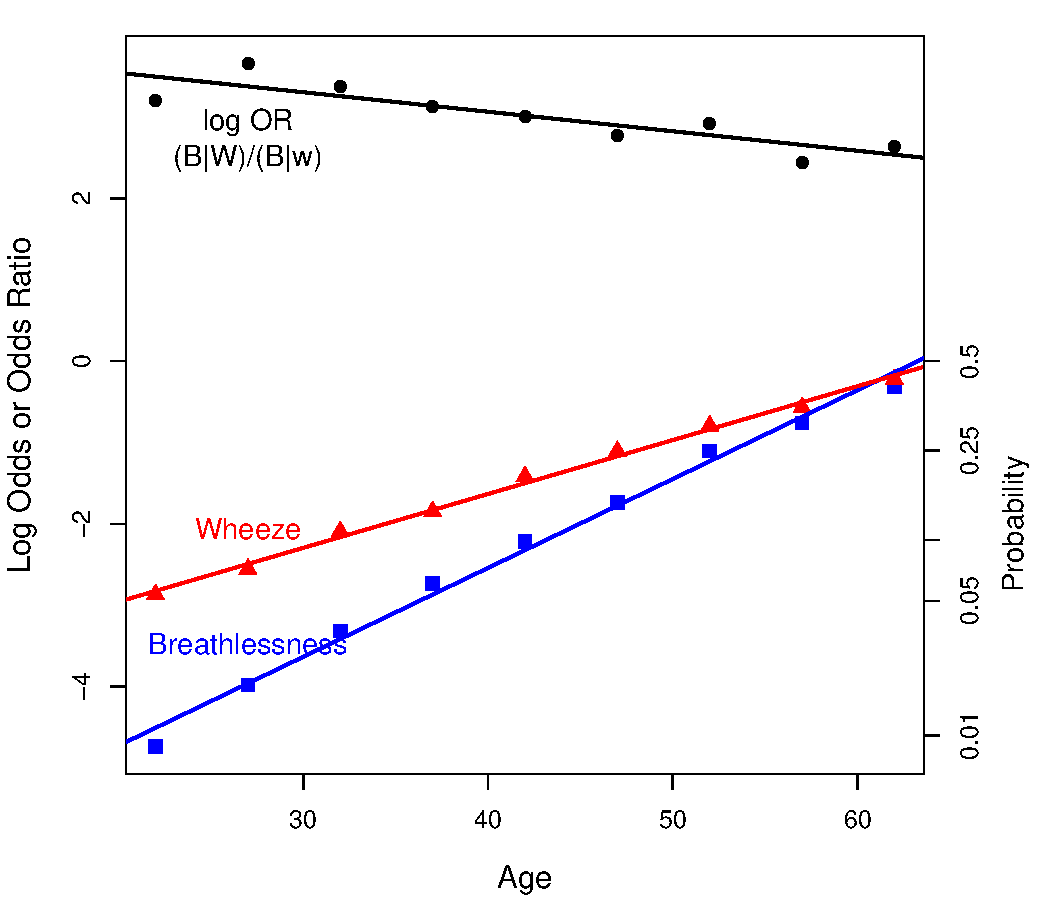
\includegraphics[width=.8\textwidth]{ch08/fig/cm-blogits-1} }

\caption[Empirical logits and log odds ratio for breathlessness and wheeze in the CoalMiners data]{Empirical logits and log odds ratio for breathlessness and wheeze in the CoalMiners data. The lines show separate linear regressions for each function. The right vertical axis shows equivalent probabilities for the logits.\label{fig:cm-blogits}}
\end{figure}


\end{knitrout}
In \figref{fig:cm-blogits}
we see that both symptoms, while quite rare among young miners, increase
steadily with age (or years working in the mine).
By age 60, the probability is nearly 0.5 of having either condition.
There is a hint of curvilinearity, particularly in the logit for
breathlessness.
The decline in the odds ratio with age may reflect selection, as miners
who had retired for health or other reasons were excluded from the
study.

\subsubsection*{Fitting \code{glm} models}
Next, we illustrate what can easily be achieved using the standard \func{glm}
approach for \loglin models and why the bivariate models we described
are more useful in this situation.  \func{glm} requires a data frame as
input, so first reshape \data{CoalMiners} to a frequency data frame.
For convenience, we simplify the variable names to \code{B} and \code{W}.

\begin{knitrout}
\definecolor{shadecolor}{rgb}{1, 0.961, 0.933}\color{fgcolor}\begin{kframe}
\begin{alltt}
\hlstd{CM} \hlkwb{<-} \hlkwd{as.data.frame}\hlstd{(CoalMiners)}
\hlkwd{colnames}\hlstd{(CM)[}\hlnum{1}\hlopt{:}\hlnum{2}\hlstd{]} \hlkwb{<-} \hlkwd{c}\hlstd{(}\hlstr{"B"}\hlstd{,} \hlstr{"W"}\hlstd{)}
\hlkwd{str}\hlstd{(CM)}
\end{alltt}
\begin{verbatim}
## 'data.frame':	36 obs. of  4 variables:
##  $ B   : Factor w/ 2 levels "B","NoB": 1 2 1 2 1 2 1 2 1 2 ...
##  $ W   : Factor w/ 2 levels "W","NoW": 1 1 2 2 1 1 2 2 1 1 ...
##  $ Age : Factor w/ 9 levels "20-24","25-29",..: 1 1 1 1 2 2 2 2 3 3 ...
##  $ Freq: num  9 95 7 1841 23 ...
\end{verbatim}
\end{kframe}
\end{knitrout}

As a point of comparison, we fit the mutual independence model, \LLM{B,W,Age}
and the baseline model for associated responses, \LLM{BW,Age}
which asserts that the association between \code{B} and {W} is
independent of \code{Age}.
\begin{knitrout}
\definecolor{shadecolor}{rgb}{1, 0.961, 0.933}\color{fgcolor}\begin{kframe}
\begin{alltt}
\hlstd{cm.glm0} \hlkwb{<-} \hlkwd{glm}\hlstd{(Freq} \hlopt{~} \hlstd{B} \hlopt{+} \hlstd{W} \hlopt{+} \hlstd{Age,} \hlkwc{data}\hlstd{=CM,} \hlkwc{family}\hlstd{=poisson)}
\hlstd{cm.glm1} \hlkwb{<-} \hlkwd{glm}\hlstd{(Freq} \hlopt{~} \hlstd{B} \hlopt{*} \hlstd{W} \hlopt{+} \hlstd{Age,} \hlkwc{data}\hlstd{=CM,} \hlkwc{family}\hlstd{=poisson)}
\hlstd{vcdExtra::}\hlkwd{Summarise}\hlstd{(cm.glm0, cm.glm1)}
\end{alltt}
\begin{verbatim}
## Likelihood summary table:
##          AIC  BIC LR Chisq Df Pr(>Chisq)    
## cm.glm0 7217 7234     6939 25     <2e-16 ***
## cm.glm1 2981 3000     2702 24     <2e-16 ***
## ---
## Signif. codes:  0 '***' 0.001 '**' 0.01 '*' 0.05 '.' 0.1 ' ' 1
\end{verbatim}
\end{kframe}
\end{knitrout}

The baseline model \code{cm.glm1}
fits very badly.  We can see the pattern of the residual association in
a mosaic display for this model shown in \figref{fig:cm-mosaic1}.
The formula argument here specifies the order of the variables in the mosaic.
\begin{knitrout}
\definecolor{shadecolor}{rgb}{1, 0.961, 0.933}\color{fgcolor}\begin{kframe}
\begin{alltt}
\hlstd{vnames} \hlkwb{<-} \hlkwd{list}\hlstd{(}\hlkwc{set_varnames} \hlstd{=} \hlkwd{c}\hlstd{(}\hlkwc{B}\hlstd{=}\hlstr{"Breathlessness"}\hlstd{,} \hlkwc{W}\hlstd{=}\hlstr{"Wheeze"}\hlstd{))}
\hlstd{lnames} \hlkwb{<-} \hlkwd{list}\hlstd{(}\hlkwc{B}\hlstd{=}\hlkwd{c}\hlstd{(}\hlstr{"B"}\hlstd{,} \hlstr{"b"}\hlstd{),} \hlkwc{W} \hlstd{=} \hlkwd{c}\hlstd{(}\hlstr{"W"}\hlstd{,} \hlstr{"w"}\hlstd{))}
\hlkwd{mosaic}\hlstd{(cm.glm1,} \hlopt{~} \hlstd{Age} \hlopt{+} \hlstd{B} \hlopt{+} \hlstd{W,}
       \hlkwc{labeling_args}\hlstd{=vnames,} \hlkwc{set_labels}\hlstd{=lnames)}
\end{alltt}
\end{kframe}\begin{figure}[!htbp]


\centerline{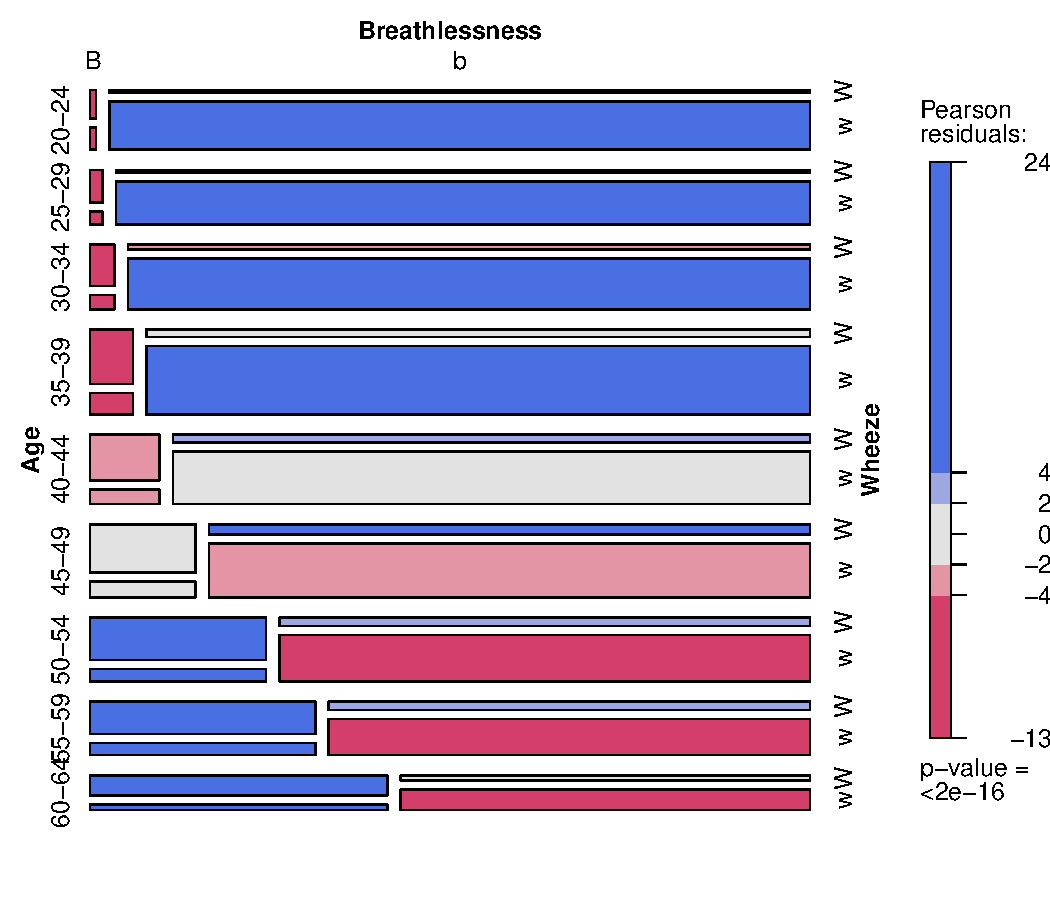
\includegraphics[width=.7\textwidth]{ch08/fig/cm-mosaic1-1} }

\caption[Mosaic display for the baseline model, BW Age, fit to the CoalMiners data]{Mosaic display for the baseline model, [BW][Age], fit to the CoalMiners data\label{fig:cm-mosaic1}}
\end{figure}


\end{knitrout}
\noindent As structured here, it is easy to see the increase in the prevalence of
breathlessness and wheeze with age and the changing pattern of their association
with age.

From \figref{fig:cm-blogits} and \figref{fig:cm-mosaic1},
it is apparent that both breathlessness and wheeze increase with age,
so we can model this by adding terms \LLM{B Age, W Age} to the baseline model.
This is the no-three-way interaction model, which could also be specified
as \verb|Freq ~ (B + W + Age)^2|.
\begin{knitrout}
\definecolor{shadecolor}{rgb}{1, 0.961, 0.933}\color{fgcolor}\begin{kframe}
\begin{alltt}
\hlstd{cm.glm2} \hlkwb{<-} \hlkwd{glm}\hlstd{(Freq} \hlopt{~} \hlstd{B} \hlopt{*} \hlstd{W} \hlopt{+} \hlstd{(B} \hlopt{+} \hlstd{W)} \hlopt{*} \hlstd{Age,} \hlkwc{data}\hlstd{=CM,} \hlkwc{family}\hlstd{=poisson)}
\hlstd{vcdExtra::}\hlkwd{Summarise}\hlstd{(cm.glm1, cm.glm2)}
\end{alltt}
\begin{verbatim}
## Likelihood summary table:
##          AIC  BIC LR Chisq Df Pr(>Chisq)    
## cm.glm1 2981 3000     2702 24     <2e-16 ***
## cm.glm2  338  383       27  8      8e-04 ***
## ---
## Signif. codes:  0 '***' 0.001 '**' 0.01 '*' 0.05 '.' 0.1 ' ' 1
\end{verbatim}
\end{kframe}
\end{knitrout}
The improvement in fit is substantial, and all terms are highly significant,
yet, the residual $G^2 (8)$ indicates there is still lack of fit.
\begin{knitrout}
\definecolor{shadecolor}{rgb}{1, 0.961, 0.933}\color{fgcolor}\begin{kframe}
\begin{alltt}
\hlkwd{library}\hlstd{(car)}
\hlkwd{Anova}\hlstd{(cm.glm2)}
\end{alltt}
\begin{verbatim}
## Analysis of Deviance Table (Type II tests)
## 
## Response: Freq
##       LR Chisq Df Pr(>Chisq)    
## B        11026  1     <2e-16 ***
## W         7038  1     <2e-16 ***
## Age        887  8     <2e-16 ***
## B:W       3025  1     <2e-16 ***
## B:Age     1130  8     <2e-16 ***
## W:Age      333  8     <2e-16 ***
## ---
## Signif. codes:  0 '***' 0.001 '**' 0.01 '*' 0.05 '.' 0.1 ' ' 1
\end{verbatim}
\end{kframe}
\end{knitrout}

One way to improve the model using the \func{glm} framework
is to make use of \var{Age} as a quantitative
variable and add a term to allow the odds ratio for the [BW] association
to vary linearly with age.  Here, we construct the variable \var{age}
using the midpoints of the Age intervals.
\begin{knitrout}
\definecolor{shadecolor}{rgb}{1, 0.961, 0.933}\color{fgcolor}\begin{kframe}
\begin{alltt}
\hlstd{CM}\hlopt{$}\hlstd{age} \hlkwb{<-} \hlkwd{rep}\hlstd{(}\hlkwd{seq}\hlstd{(}\hlnum{22}\hlstd{,} \hlnum{62}\hlstd{,} \hlnum{5}\hlstd{),} \hlkwc{each}\hlstd{=}\hlnum{4}\hlstd{)}
\end{alltt}
\end{kframe}
\end{knitrout}
In the \func{glm} approach, the odds ratio cannot be modeled directly, but we
can use the following trick: For each $2 \times 2$ subtable, the odds ratio
can be parameterized in terms of the frequency in any one cell, say,
$n_{11k}$, given that the marginal total $n_{++k}$ is included in the model.
We do this by adding a new interaction variable, \var{ageOR} having the value
of \var{age} for the $(1, 1, k)$ cells and 0 otherwise.
\begin{knitrout}
\definecolor{shadecolor}{rgb}{1, 0.961, 0.933}\color{fgcolor}\begin{kframe}
\begin{alltt}
\hlstd{CM}\hlopt{$}\hlstd{ageOR} \hlkwb{<-} \hlstd{(CM}\hlopt{$}\hlstd{B}\hlopt{==}\hlstr{"B"}\hlstd{)} \hlopt{*} \hlstd{(CM}\hlopt{$}\hlstd{W}\hlopt{==}\hlstr{"W"}\hlstd{)} \hlopt{*} \hlstd{CM}\hlopt{$}\hlstd{age}
\hlstd{cm.glm3} \hlkwb{<-} \hlkwd{update}\hlstd{(cm.glm2, .} \hlopt{~} \hlstd{.} \hlopt{+} \hlstd{ageOR)}
\hlstd{vcdExtra::}\hlkwd{Summarise}\hlstd{(cm.glm0, cm.glm1, cm.glm2, cm.glm3)}
\end{alltt}
\begin{verbatim}
## Likelihood summary table:
##          AIC  BIC LR Chisq Df Pr(>Chisq)    
## cm.glm0 7217 7234     6939 25     <2e-16 ***
## cm.glm1 2981 3000     2702 24     <2e-16 ***
## cm.glm2  338  383       27  8     0.0008 ***
## cm.glm3  320  366        7  7     0.4498    
## ---
## Signif. codes:  0 '***' 0.001 '**' 0.01 '*' 0.05 '.' 0.1 ' ' 1
\end{verbatim}
\end{kframe}
\end{knitrout}
\noindent The model \code{cm.glm3}, with one more parameter, now fits reasonably
well, having residual $G^2 (7) = 6.80$.
The likelihood ratio test of
model \code{cm.glm3} against \code{cm.glm2}, which assumes equal odds
ratios over age, can be regarded as a test of the hypothesis of
homogeneity of odds ratios, against the alternative that the [BW] association
changes linearly with age.  
The \func{glm} models fit in this example are summarized above.
As usual, \func{anova} can be used to compare competing nested models.
\begin{knitrout}
\definecolor{shadecolor}{rgb}{1, 0.961, 0.933}\color{fgcolor}\begin{kframe}
\begin{alltt}
\hlkwd{anova}\hlstd{(cm.glm2, cm.glm3,} \hlkwc{test}\hlstd{=}\hlstr{"Chisq"}\hlstd{)}
\end{alltt}
\begin{verbatim}
## Analysis of Deviance Table
## 
## Model 1: Freq ~ B * W + (B + W) * Age
## Model 2: Freq ~ B + W + Age + ageOR + B:W + B:Age + W:Age
##   Resid. Df Resid. Dev Df Deviance Pr(>Chi)    
## 1         8       26.7                         
## 2         7        6.8  1     19.9  8.2e-06 ***
## ---
## Signif. codes:  0 '***' 0.001 '**' 0.01 '*' 0.05 '.' 0.1 ' ' 1
\end{verbatim}
\end{kframe}
\end{knitrout}

This analysis, while useful, also shows the limitations of the \func{glm} approach:
\begin{seriate}
  \item It doesn't easily allow us to represent and test the substantively interesting
  hypotheses regarding \emph{how} the prevalence of the binary responses, \code{B} and
  \code{W} vary with \code{Age}, such as seen in \figref{fig:cm-blogits}.
  \item It doesn't represent the odds ratio for the \LLM{BW} association directly,
  but only through the coding trick we used here.  Thus, it is difficult to interpret
  the coefficient for \code{ageOR} = -0.02613 in a substantively
  meaningful way, except that is shows that the odds ratio is decreasing.%
\footnote{
Actually, the interpretability of the coefficient for the log odds ratio can be
enhanced here by centering age, and representing its units in steps of 5 years,
as we do below.
}
\end{seriate}

\subsubsection*{Fitting \code{vglm} models}
The \func{vglm} function in the \Rpackage{VGAM} provides a very general implementation of these
and other models for discrete multivariate responses. The family function,
\func{binom2.or} for binary logistic models allows some or all of the logits or
odds ratio submodels to be constrained to be intercept-only (e.g., as in \eqref{eq:bilogit1})
and the two marginal distributions can be constrained to be equal.

Quantitative predictors (such as age, here), can be modeled linearly or
nonlinearly, using \func{poly} for a parametric fit, or smooth regression splines,
as provided by the functions \func{ns}, \func{bs} and others in model formulas.
In this illustration, we fit bivariate linear and quadratic models in age.

\func{vglm} takes its input data in the wide form we called \code{coalminers} at the beginning
of this example.  We could use the 9-level factor, \var{Age} as we did with \func{glm},
but we plan to use \var{age} as a numeric variable in all three submodels.  The coefficients
in these models will be more easily interpreted if we center age and express it
as \code{agec} in units of five years, as shown below.

\begin{knitrout}
\definecolor{shadecolor}{rgb}{1, 0.961, 0.933}\color{fgcolor}\begin{kframe}
\begin{alltt}
\hlstd{coalminers} \hlkwb{<-} \hlkwd{transform}\hlstd{(coalminers,} \hlkwc{agec}\hlstd{=(age}\hlopt{-}\hlnum{42}\hlstd{)}\hlopt{/}\hlnum{5}\hlstd{)}
\hlstd{coalminers}\hlopt{$}\hlstd{Age} \hlkwb{<-} \hlkwd{dimnames}\hlstd{(CoalMiners)[[}\hlnum{3}\hlstd{]]}
\hlstd{coalminers}
\end{alltt}
\begin{verbatim}
##    BW  Bw  bW   bw age agec   Age
## 1   9   7  95 1841  22   -4 20-24
## 2  23   9 105 1654  27   -3 25-29
## 3  54  19 177 1863  32   -2 30-34
## 4 121  48 257 2357  37   -1 35-39
## 5 169  54 273 1778  42    0 40-44
## 6 269  88 324 1712  47    1 45-49
## 7 404 117 245 1324  52    2 50-54
## 8 406 152 225  967  57    3 55-59
## 9 372 106 132  526  62    4 60-64
\end{verbatim}
\end{kframe}
\end{knitrout}
\func{vglm} takes the $2 \times 2$ response frequencies as a 4-column matrix on the right
hand side of the model formula.  However, denoting the responses of
failure and success by 0 and 1 respectively,
it takes these in the order $y_{00}, y_{01}, y_{10}, y_{11}$.
We specify the order below so that the logits are calculated for the
occurrence of breathlessness or wheeze, rather than their absence.
\begin{knitrout}
\definecolor{shadecolor}{rgb}{1, 0.961, 0.933}\color{fgcolor}\begin{kframe}
\begin{alltt}
\hlkwd{library}\hlstd{(VGAM)}
\hlcom{#                      00  01  10  11}
\hlstd{cm.vglm1} \hlkwb{<-} \hlkwd{vglm}\hlstd{(}\hlkwd{cbind}\hlstd{(bw, bW, Bw, BW)} \hlopt{~} \hlstd{agec,}
                 \hlkwd{binom2.or}\hlstd{(}\hlkwc{zero}\hlstd{=}\hlkwa{NULL}\hlstd{),} \hlkwc{data}\hlstd{=coalminers)}
\hlstd{cm.vglm1}
\end{alltt}
\begin{verbatim}
## Call:
## vglm(formula = cbind(bw, bW, Bw, BW) ~ agec, family = binom2.or(zero = NULL), 
##     data = coalminers)
## 
## Coefficients:
## (Intercept):1 (Intercept):2 (Intercept):3        agec:1 
##      -2.26247      -1.48776       3.02191       0.51451 
##        agec:2        agec:3 
##       0.32545      -0.13136 
## 
## Degrees of Freedom: 27 Total; 21 Residual
## Residual deviance: 30.394 
## Log-likelihood: -100.53
\end{verbatim}
\end{kframe}
\end{knitrout}
\noindent In this call, the argument \code{zero=NULL} indicates that none of the
linear predictors, $\eta_1, \eta_2, \eta_{12}$ are modeled as constants.%
\footnote{
The default, \code{zero=3} gives the model shown in \eqref{eq:bilogit1},
with the odds ratio constant.
}

At this writing, there is no \func{anova} method for the \class{vgam} objects
produced by \func{vglm}, but we can test the residual deviance of the model
(against the saturated model) as follows, showing that this model has
an acceptable fit.
\begin{knitrout}
\definecolor{shadecolor}{rgb}{1, 0.961, 0.933}\color{fgcolor}\begin{kframe}
\begin{alltt}
\hlstd{(G2} \hlkwb{<-} \hlkwd{deviance}\hlstd{(cm.vglm1))}
\end{alltt}
\begin{verbatim}
## [1] 30.394
\end{verbatim}
\begin{alltt}
\hlcom{# test residual deviance}
\hlnum{1}\hlopt{-}\hlkwd{pchisq}\hlstd{(}\hlkwd{deviance}\hlstd{(cm.vglm1), cm.vglm1}\hlopt{@}\hlkwc{df.residual}\hlstd{)}
\end{alltt}
\begin{verbatim}
## [1] 0.084355
\end{verbatim}
\end{kframe}
\end{knitrout}


The estimated coefficients in this model are usefully shown as below, using the
argument \code{matrix=TRUE} in \func{coef}.
Using \func{exp}
on the result gives values of odds that can be easily interpreted:
\begin{knitrout}
\definecolor{shadecolor}{rgb}{1, 0.961, 0.933}\color{fgcolor}\begin{kframe}
\begin{alltt}
\hlkwd{coef}\hlstd{(cm.vglm1,} \hlkwc{matrix}\hlstd{=}\hlnum{TRUE}\hlstd{)}
\end{alltt}
\begin{verbatim}
##             logit(mu1) logit(mu2) log(oratio)
## (Intercept)   -2.26247   -1.48776     3.02191
## agec           0.51451    0.32545    -0.13136
\end{verbatim}
\begin{alltt}
\hlkwd{exp}\hlstd{(}\hlkwd{coef}\hlstd{(cm.vglm1,} \hlkwc{matrix}\hlstd{=}\hlnum{TRUE}\hlstd{))}
\end{alltt}
\begin{verbatim}
##             logit(mu1) logit(mu2) log(oratio)
## (Intercept)    0.10409    0.22588     20.5304
## agec           1.67282    1.38465      0.8769
\end{verbatim}
\end{kframe}
\end{knitrout}
Thus, the odds of a miner showing breathlessness are multiplied by 1.67, a 67\% increase,
for each 5 years increase in age;  similarly, the odds of wheeze are multiplied by 1.38,
a 38\% increase. The odds ratio for the association between the two symptoms are multiplied
by 0.88, a 12\% decrease over each 5 year interval.


The \Rpackage{VGAM} has no special plot methods for \class{vglm} objects, but
it is not hard to construct these using the methods we showed earlier in this example.
First, we can obtain the fitted probabilities for the 4 response combinations using
\func{fitted} and the corresponding observed probabilities using \func{depvar}.
\begin{knitrout}
\definecolor{shadecolor}{rgb}{1, 0.961, 0.933}\color{fgcolor}\begin{kframe}
\begin{alltt}
\hlstd{age} \hlkwb{<-} \hlstd{coalminers}\hlopt{$}\hlstd{age}
\hlstd{P} \hlkwb{<-} \hlkwd{fitted}\hlstd{(cm.vglm1)}
\hlkwd{colnames}\hlstd{(P)} \hlkwb{<-} \hlkwd{c}\hlstd{(}\hlstr{"bw"}\hlstd{,} \hlstr{"bW"}\hlstd{,} \hlstr{"Bw"}\hlstd{,} \hlstr{"BW"}\hlstd{)}
\hlkwd{head}\hlstd{(P)}
\end{alltt}
\begin{verbatim}
##        bw       bW        Bw        BW
## 1 0.93747 0.049409 0.0046356 0.0084831
## 2 0.91461 0.063636 0.0069757 0.0147776
## 3 0.88411 0.080029 0.0104965 0.0253679
## 4 0.84394 0.097484 0.0158138 0.0427671
## 5 0.79188 0.113839 0.0238598 0.0704196
## 6 0.72578 0.125910 0.0359684 0.1123366
\end{verbatim}
\begin{alltt}
\hlstd{Y} \hlkwb{<-} \hlkwd{depvar}\hlstd{(cm.vglm1)}
\end{alltt}
\end{kframe}
\end{knitrout}
\begin{figure}
\centering
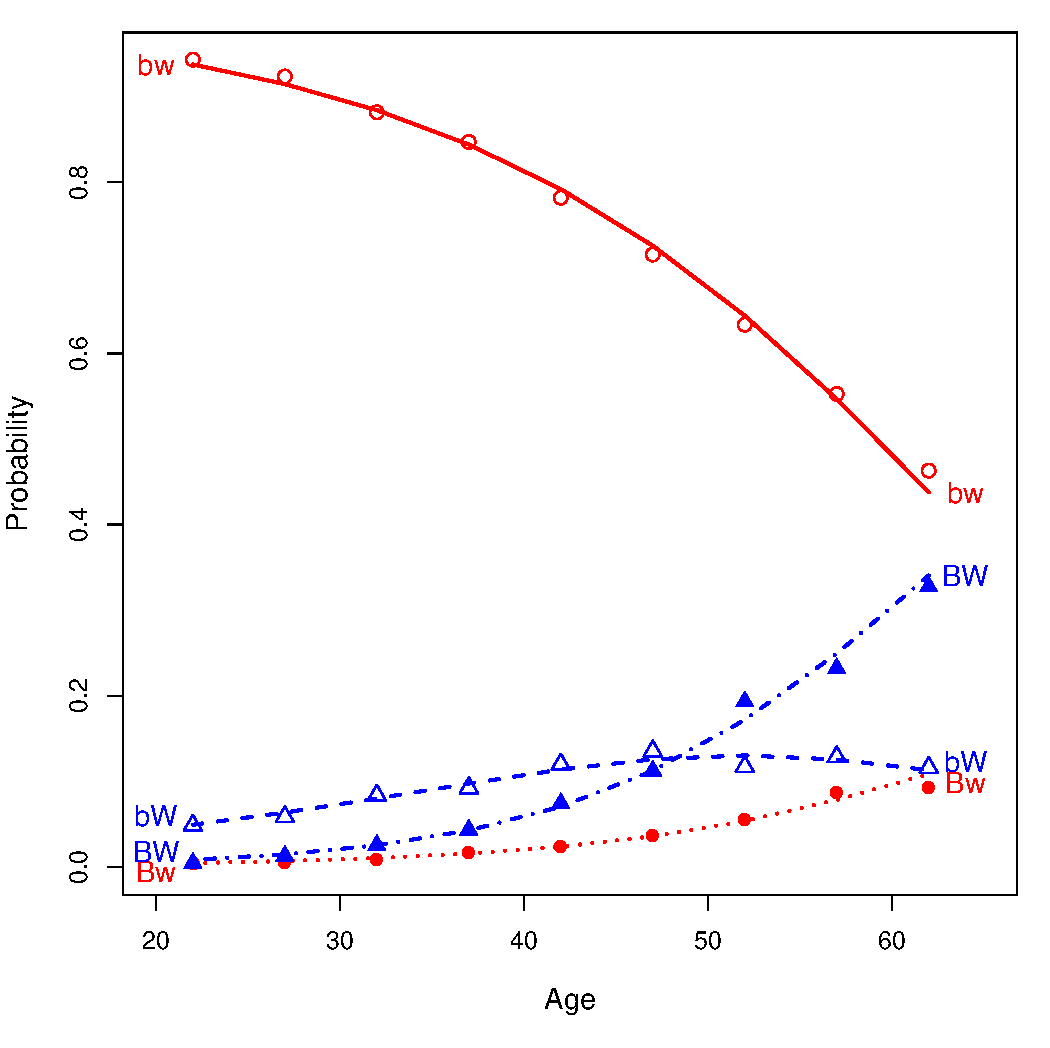
\includegraphics[width=.49\textwidth]{ch08/fig/cm-vglm1-prob}
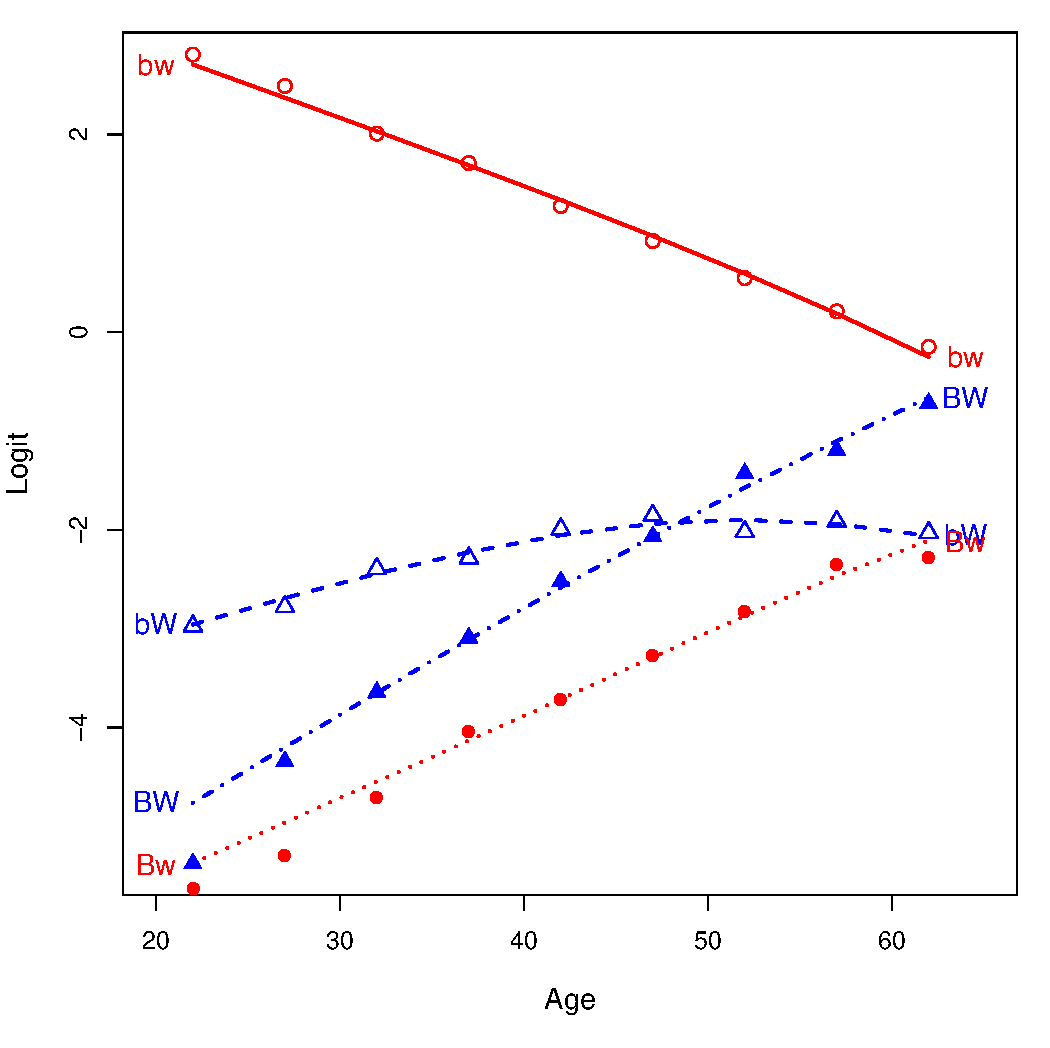
\includegraphics[width=.49\textwidth]{ch08/fig/cm-vglm1-logit}
\caption{Observed and fitted values for the combinations of breathlessness and wheeze in the binary logistic regression model \code{cm.vglm1}. Left: probabilities; right: on the log odds scale.}
\label{fig:cm-vglm1}
\end{figure}

In the left panel of \figref{fig:cm-vglm1}, we plot the fitted probabilities in the matrix
\code{P} using \func{matplot} and the observed probabilities in \code{Y} using \func{matpoints}.

\begin{knitrout}
\definecolor{shadecolor}{rgb}{1, 0.961, 0.933}\color{fgcolor}\begin{kframe}
\begin{alltt}
\hlstd{col} \hlkwb{<-} \hlkwd{c}\hlstd{(}\hlstr{"red"}\hlstd{,} \hlstr{"blue"}\hlstd{,} \hlstr{"red"}\hlstd{,} \hlstr{"blue"}\hlstd{)}
\hlstd{pch} \hlkwb{<-} \hlkwd{c}\hlstd{(}\hlnum{1}\hlstd{,}\hlnum{2}\hlstd{,}\hlnum{16}\hlstd{,}\hlnum{17}\hlstd{)}

\hlstd{op} \hlkwb{<-} \hlkwd{par}\hlstd{(}\hlkwc{mar}\hlstd{=}\hlkwd{c}\hlstd{(}\hlnum{5}\hlstd{,}\hlnum{4}\hlstd{,}\hlnum{1}\hlstd{,}\hlnum{1}\hlstd{)}\hlopt{+}\hlnum{.1}\hlstd{)}
\hlkwd{matplot}\hlstd{(age, P,} \hlkwc{type}\hlstd{=}\hlstr{"l"}\hlstd{,}
  \hlkwc{col}\hlstd{=col,}
  \hlkwc{lwd}\hlstd{=}\hlnum{2}\hlstd{,} \hlkwc{cex}\hlstd{=}\hlnum{1.2}\hlstd{,} \hlkwc{cex.lab}\hlstd{=}\hlnum{1.2}\hlstd{,}
  \hlkwc{xlab}\hlstd{=}\hlstr{"Age"}\hlstd{,} \hlkwc{ylab}\hlstd{=}\hlstr{"Probability"}\hlstd{,}
  \hlkwc{xlim}\hlstd{=}\hlkwd{c}\hlstd{(}\hlnum{20}\hlstd{,}\hlnum{65}\hlstd{))}
\hlkwd{matpoints}\hlstd{(age, Y,}
  \hlkwc{pch}\hlstd{=pch,} \hlkwc{cex}\hlstd{=}\hlnum{1.2}\hlstd{,} \hlkwc{col}\hlstd{=col)}
\hlcom{# legend}
\hlkwd{text}\hlstd{(}\hlnum{64}\hlstd{, P[}\hlnum{9}\hlstd{,]}\hlopt{+} \hlkwd{c}\hlstd{(}\hlnum{0}\hlstd{,}\hlnum{.01}\hlstd{,} \hlopt{-}\hlnum{.01}\hlstd{,} \hlnum{0}\hlstd{),} \hlkwc{labels}\hlstd{=}\hlkwd{colnames}\hlstd{(P),} \hlkwc{col}\hlstd{=col,} \hlkwc{cex}\hlstd{=}\hlnum{1.2}\hlstd{)}
\hlkwd{text}\hlstd{(}\hlnum{20}\hlstd{, P[}\hlnum{1}\hlstd{,]}\hlopt{+} \hlkwd{c}\hlstd{(}\hlnum{0}\hlstd{,}\hlnum{.01}\hlstd{,} \hlopt{-}\hlnum{.01}\hlstd{,} \hlnum{.01}\hlstd{),} \hlkwc{labels}\hlstd{=}\hlkwd{colnames}\hlstd{(P),} \hlkwc{col}\hlstd{=col,} \hlkwc{cex}\hlstd{=}\hlnum{1.2}\hlstd{)}
\hlkwd{par}\hlstd{(op)}
\end{alltt}
\end{kframe}
\end{knitrout}
The right panel of \figref{fig:cm-vglm1} shows these on the log odds scale, produced
using the same code as above, applied to the probabilities transformed using \func{qlogis},
the quantile function for the logistic distribution.
\begin{knitrout}
\definecolor{shadecolor}{rgb}{1, 0.961, 0.933}\color{fgcolor}\begin{kframe}
\begin{alltt}
\hlstd{lP} \hlkwb{<-} \hlkwd{qlogis}\hlstd{(P)}
\hlstd{lY} \hlkwb{<-} \hlkwd{qlogis}\hlstd{(Y)}
\end{alltt}
\end{kframe}
\end{knitrout}
In \figref{fig:cm-blogits} we plotted the empirical logits and log odds using the
function \func{blogits} to transform frequencies to these values.  An essentially
identical plot can be produced by transforming the fitted and observed probabilities,
as calculated below.
\begin{knitrout}
\definecolor{shadecolor}{rgb}{1, 0.961, 0.933}\color{fgcolor}\begin{kframe}
\begin{alltt}
\hlcom{# blogits, but for B and W}
\hlstd{logitsP} \hlkwb{<-} \hlkwd{blogits}\hlstd{(P[,}\hlnum{4}\hlopt{:}\hlnum{1}\hlstd{])}
\hlstd{logitsY} \hlkwb{<-} \hlkwd{blogits}\hlstd{(Y[,}\hlnum{4}\hlopt{:}\hlnum{1}\hlstd{])}
\end{alltt}
\end{kframe}
\end{knitrout}

To test for nonlinearity in the prevalence of the symptoms or their odds ratio with
age, we can fit a similar model using \func{poly} or a smoothing spline, such as
\func{ns}.  We illustrate this here using a bivariate model allowing quadratic
effects of age on all three components.

\begin{knitrout}
\definecolor{shadecolor}{rgb}{1, 0.961, 0.933}\color{fgcolor}\begin{kframe}
\begin{alltt}
\hlstd{cm.vglm2} \hlkwb{<-} \hlkwd{vglm}\hlstd{(}\hlkwd{cbind}\hlstd{(bw, bW, Bw, BW)} \hlopt{~} \hlkwd{poly}\hlstd{(agec,}\hlnum{2}\hlstd{),}
                 \hlkwd{binom2.or}\hlstd{(}\hlkwc{zero}\hlstd{=}\hlkwa{NULL}\hlstd{),} \hlkwc{data}\hlstd{=coalminers)}
\end{alltt}
\end{kframe}
\end{knitrout}

This model has a residual $G^2=$ 16.963 with 18
df.  Compared to the linear model \code{cm.vglm1}, this represents a significant
improvement in goodness of fit.

\begin{knitrout}
\definecolor{shadecolor}{rgb}{1, 0.961, 0.933}\color{fgcolor}\begin{kframe}
\begin{alltt}
\hlstd{(LR} \hlkwb{<-} \hlkwd{deviance}\hlstd{(cm.vglm1)} \hlopt{-} \hlkwd{deviance}\hlstd{(cm.vglm2))}
\end{alltt}
\begin{verbatim}
## [1] 13.43
\end{verbatim}
\begin{alltt}
\hlnum{1} \hlopt{-} \hlkwd{pchisq}\hlstd{(LR, cm.vglm1}\hlopt{@}\hlkwc{df.residual} \hlopt{-} \hlstd{cm.vglm2}\hlopt{@}\hlkwc{df.residual}\hlstd{)}
\end{alltt}
\begin{verbatim}
## [1] 0.0037925
\end{verbatim}
\end{kframe}
\end{knitrout}

A plot of the fitted logits and log odds ratios under this model is shown in \figref{fig:cm-vglm2-blogit}.
You can interpret this plot as showing that the statistical evidence for the quadratic
model indicates some slight tendency for the prevalence of breathlessness and wheeze levels off
slightly with age, particularly the former.
\begin{figure}[!htb]
\centering
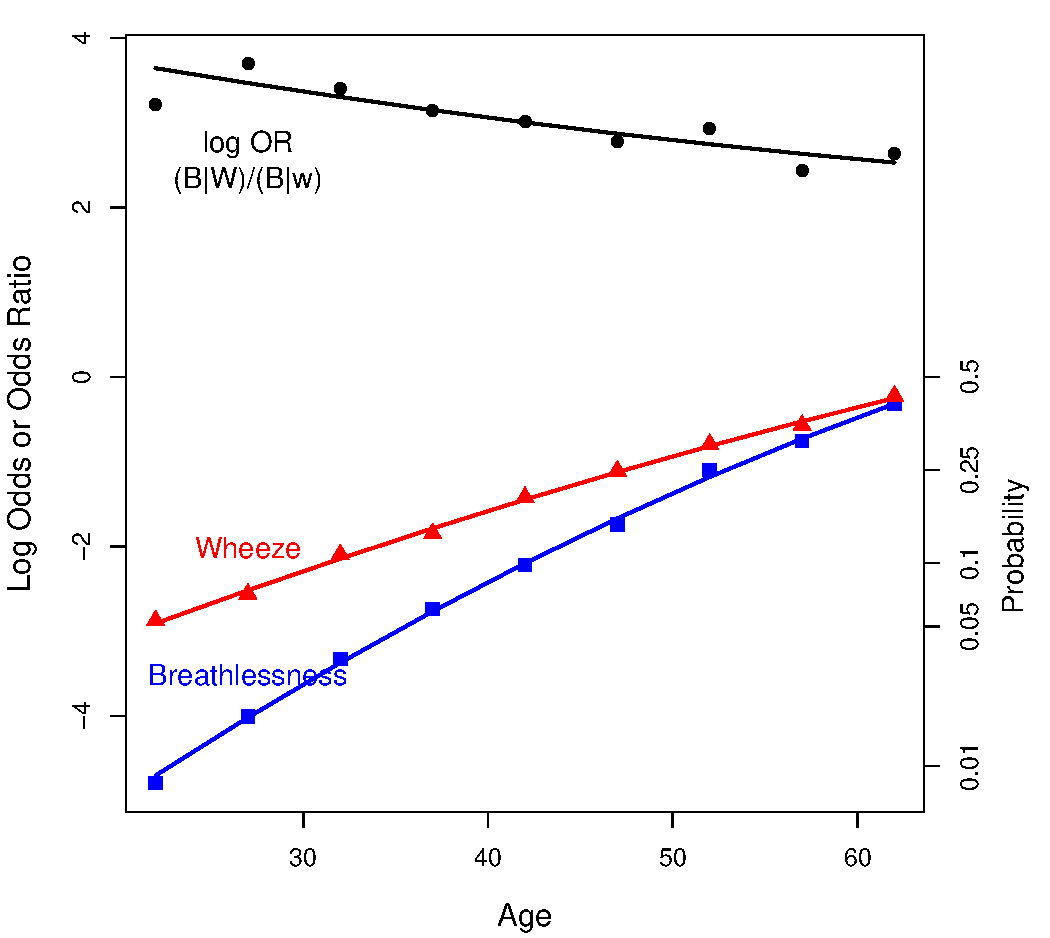
\includegraphics[width=.8\textwidth]{ch08/fig/cm-vglm2-blogit}
\caption{Observed (points) and fitted (lines) logits and log odds ratios
 for the quadratic binary logistic regression model \code{cm.vglm2}.}
\label{fig:cm-vglm2-blogit}
\end{figure}


\end{Example}

\subsection{More complex models}
When there is more than one explanatory variable and several responses,
the methods described above using \func{glm} and \func{vglm} still
apply.  However, it is useful to begin with a more thorough
visual examination of the relations within and between these sets.
Some useful graphical displays include:
\begin{itemize}
\item mosaic displays showing the marginal relations among the response variables
and of the explanatory variables, each collapsed over the other set;
\item conditional mosaics or fourfold displays of the associations among
the responses, stratified by one or more of the explanatory variables;
\item plots of empirical logits and log odds ratios, as in \figref{fig:cm-blogits}
or model-based plots, such as \figref{fig:cm-vglm2-blogit}, showing a model-smoothed
summary.
\end{itemize}
These displays can, and should, inform our search for an adequate
descriptive or explanatory model.  Some of these ideas are illustrated in the following
example.


\begin{Example}[toxaemia]{Toxaemic symptoms in pregnancy}

\citet{Brown-etal:83} gave the data used here on two signs of \emph{toxaemia},
an abnormal condition during pregnancy characterized by
high blood pressure (hypertension) and high levels of protein
in the urine.  If untreated, both the mother and baby are
at risk of complications or death.
The data frame \data{Toxaemia} in \pkg{vcdExtra}
represents 13,384 expectant
mothers in Bradford, England in their first pregnancy, who
were also classified according to social class and the number
of cigarettes smoked per day.

There are thus two response variables, and two explanatory variables
in this data set in frequency form.  For convenience, we also convert
it to a $2 \times 2 \times 5 \times 3$ table.
\begin{knitrout}\footnotesize
\definecolor{shadecolor}{rgb}{1, 0.961, 0.933}\color{fgcolor}\begin{kframe}
\begin{alltt}
\hlkwd{data}\hlstd{(}\hlstr{"Toxaemia"}\hlstd{,} \hlkwc{package}\hlstd{=}\hlstr{"vcdExtra"}\hlstd{)}
\hlkwd{str}\hlstd{(Toxaemia)}
\end{alltt}
\begin{verbatim}
## 'data.frame':	60 obs. of  5 variables:
##  $ class: Factor w/ 5 levels "1","2","3","4",..: 1 1 1 1 1 1 1 1 1 1 ...
##  $ smoke: Factor w/ 3 levels "0","1-19","20+": 1 1 1 1 2 2 2 2 3 3 ...
##  $ hyper: Factor w/ 2 levels "Low","High": 2 2 1 1 2 2 1 1 2 2 ...
##  $ urea : Factor w/ 2 levels "Low","High": 2 1 2 1 2 1 2 1 2 1 ...
##  $ Freq : int  28 82 21 286 5 24 5 71 1 3 ...
\end{verbatim}
\begin{alltt}
\hlstd{tox.tab} \hlkwb{<-} \hlkwd{xtabs}\hlstd{(Freq}\hlopt{~}\hlstd{class} \hlopt{+} \hlstd{smoke} \hlopt{+} \hlstd{hyper} \hlopt{+} \hlstd{urea, Toxaemia)}
\hlkwd{ftable}\hlstd{(tox.tab,} \hlkwc{row.vars}\hlstd{=}\hlnum{1}\hlstd{)}
\end{alltt}
\begin{verbatim}
##       smoke    0                1-19                 20+               
##       hyper  Low      High       Low      High       Low      High     
##       urea   Low High  Low High  Low High  Low High  Low High  Low High
## class                                                                  
## 1            286   21   82   28   71    5   24    5   13    0    3    1
## 2            785   34  266   50  284   17   92   13   34    3   15    0
## 3           3160  164 1101  278 2300  142  492  120  383   32   92   16
## 4            656   52  213   63  649   46  129   35  163   12   40    7
## 5            245   23   78   20  321   34   74   22   65    4   14    7
\end{verbatim}
\end{kframe}
\end{knitrout}

The questions of main interest are how the occurrence of each symptom
varies with social class and smoking, and how the association between
these symptoms varies. It is useful, however, to examine first the marginal relationship between
the two responses, and between the two predictors.
The calls to \func{mosaic} below produce the two panels in \figref{fig:tox-mosaic1}.

\begin{knitrout}
\definecolor{shadecolor}{rgb}{1, 0.961, 0.933}\color{fgcolor}\begin{kframe}
\begin{alltt}
\hlkwd{mosaic}\hlstd{(}\hlopt{~}\hlstd{smoke} \hlopt{+} \hlstd{class,} \hlkwc{data}\hlstd{=tox.tab,} \hlkwc{shade}\hlstd{=}\hlnum{TRUE}\hlstd{,}
       \hlkwc{main}\hlstd{=}\hlstr{"Predictors"}\hlstd{,} \hlkwc{legend}\hlstd{=}\hlnum{FALSE}\hlstd{)}
\hlkwd{mosaic}\hlstd{(}\hlopt{~}\hlstd{hyper} \hlopt{+} \hlstd{urea,} \hlkwc{data}\hlstd{=tox.tab,} \hlkwc{shade}\hlstd{=}\hlnum{TRUE}\hlstd{,}
       \hlkwc{main}\hlstd{=}\hlstr{"Responses"}\hlstd{,} \hlkwc{legend}\hlstd{=}\hlnum{FALSE}\hlstd{)}
\end{alltt}
\end{kframe}\begin{figure}[!htbp]


\centerline{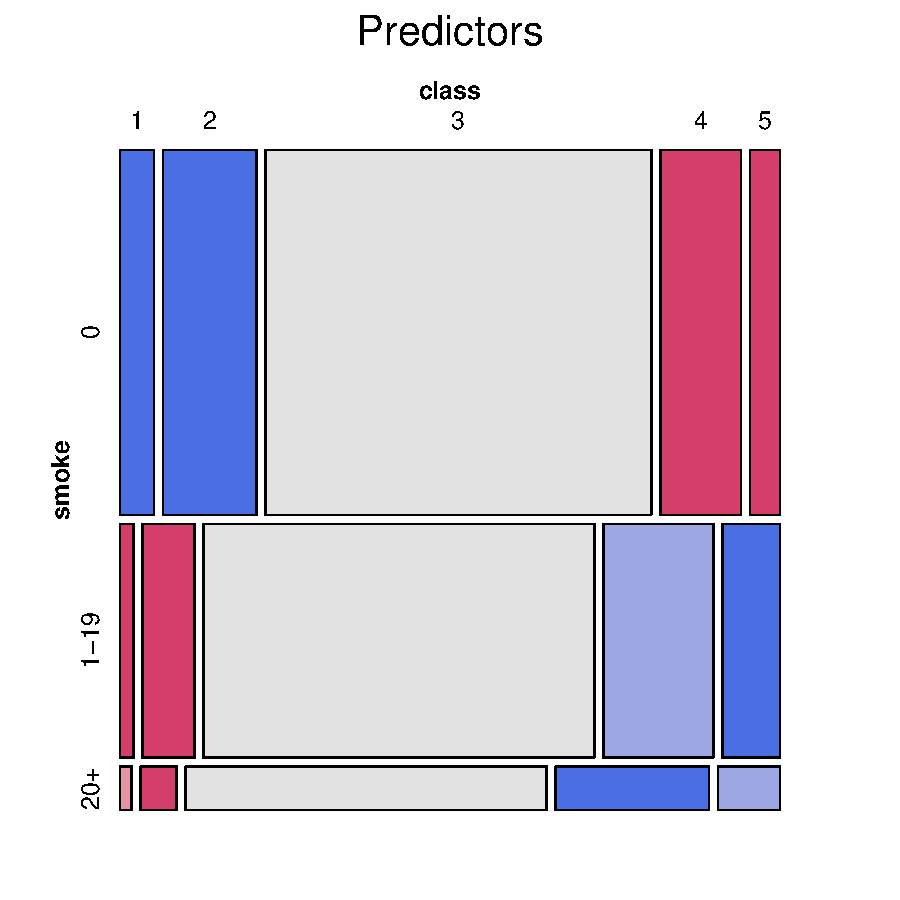
\includegraphics[width=.5\textwidth]{ch08/fig/tox-mosaic1-1} 
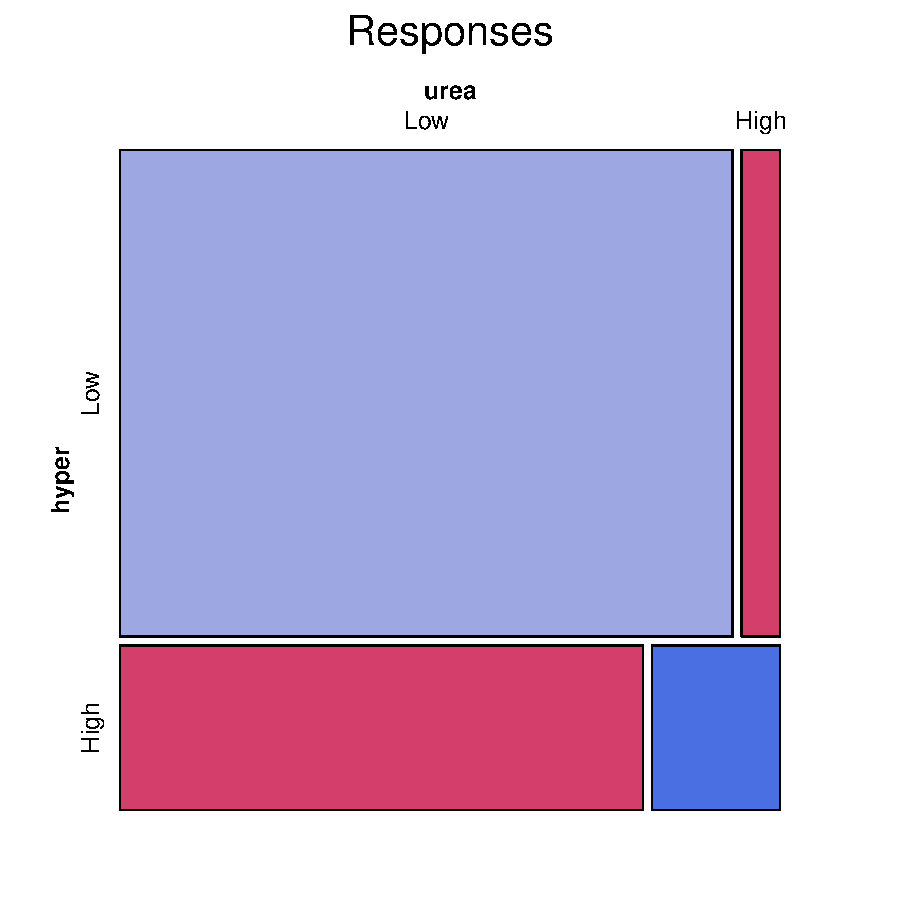
\includegraphics[width=.5\textwidth]{ch08/fig/tox-mosaic1-2} }

\caption[Mosaic displays for Toxaemia data]{Mosaic displays for Toxaemia data: Predictor and response associations\label{fig:tox-mosaic1}}
\end{figure}


\end{knitrout}
We see in \figref{fig:tox-mosaic1} that the majority of the mothers are in the
third social class, and that smoking is negatively related to social
class, with the highest levels of smoking in classes 4 and 5.
(Social class 1 is the highest in status here.)
More than 50\% are non-smokers.
Within the responses, the great majority of women exhibit neither symptom,
but showing one symptom makes it much more likely to show the other.
Marginally, hypertension is somewhat more prevalent than protein urea.

We next examine how the association between responses varies with
social class and with smoking.
\figref{fig:tox-mosaic2}  shows a collection of conditional
mosaic plots using \func{cotabplot} of the association between hypertension and urea,
for each level of smoking, collapsed over social class.

\begin{knitrout}
\definecolor{shadecolor}{rgb}{1, 0.961, 0.933}\color{fgcolor}\begin{kframe}
\begin{alltt}
\hlkwd{cotabplot}\hlstd{(}\hlopt{~}\hlstd{hyper} \hlopt{+} \hlstd{urea} \hlopt{|} \hlstd{smoke, tox.tab,} \hlkwc{shade}\hlstd{=}\hlnum{TRUE}\hlstd{,}
          \hlkwc{legend}\hlstd{=}\hlnum{FALSE}\hlstd{,} \hlkwc{layout}\hlstd{=}\hlkwd{c}\hlstd{(}\hlnum{1}\hlstd{,}\hlnum{3}\hlstd{))}
\end{alltt}
\end{kframe}\begin{figure}[!htbp]


\centerline{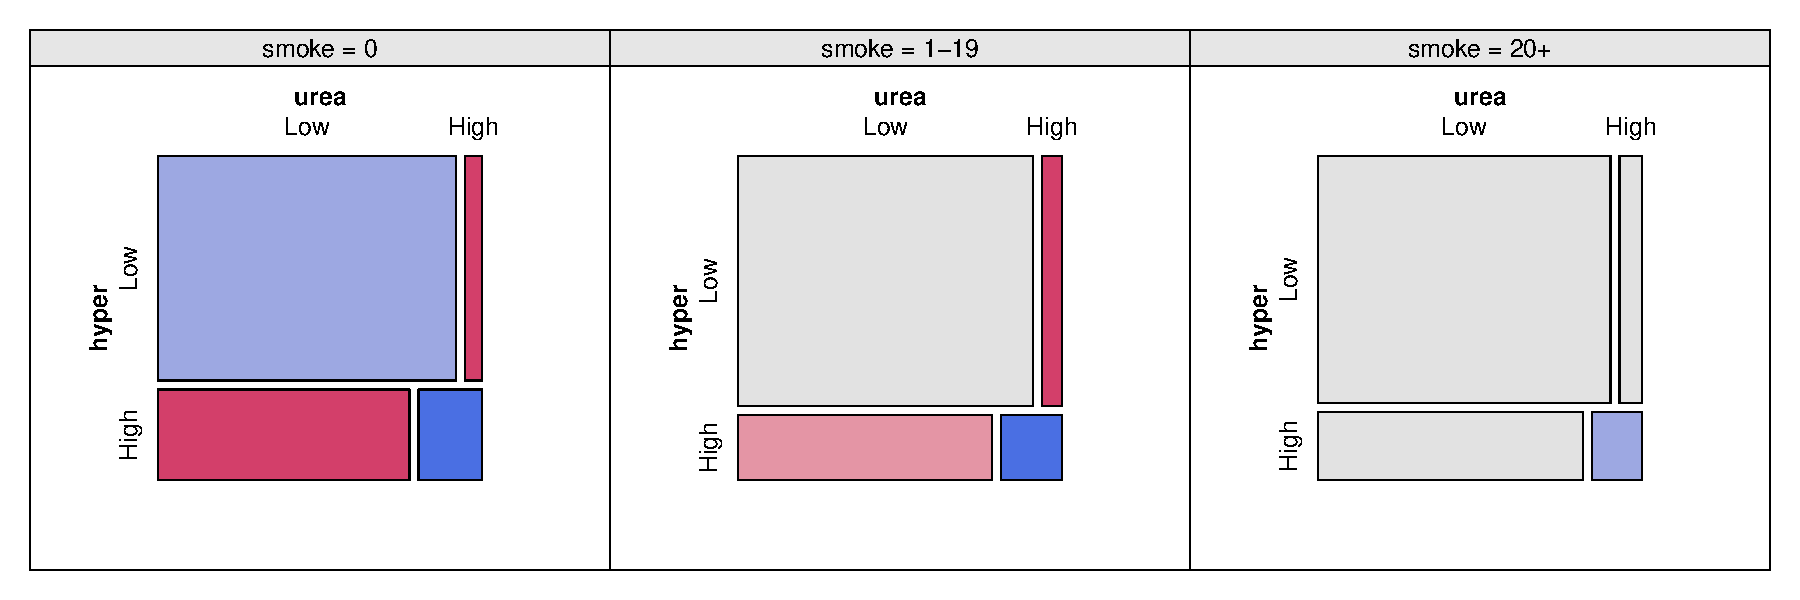
\includegraphics[width=1.1\textwidth]{ch08/fig/tox-mosaic2-1} }

\caption[Toxaemia data]{Toxaemia data: Response association conditioned on smoking level\label{fig:tox-mosaic2}}
\end{figure}


\end{knitrout}
\figref{fig:tox-mosaic3} is similar, but stratified by social class.
The marginal frequencies of the conditioning variable is not represented in these plots.
(For example, as can be seen in \figref{fig:tox-mosaic1}, the greatest number of women are in class 3.)

\begin{knitrout}
\definecolor{shadecolor}{rgb}{1, 0.961, 0.933}\color{fgcolor}\begin{kframe}
\begin{alltt}
\hlkwd{cotabplot}\hlstd{(}\hlopt{~}\hlstd{hyper} \hlopt{+} \hlstd{urea} \hlopt{|} \hlstd{class, tox.tab,} \hlkwc{shade}\hlstd{=}\hlnum{TRUE}\hlstd{,}
          \hlkwc{legend}\hlstd{=}\hlnum{FALSE}\hlstd{,} \hlkwc{layout}\hlstd{=}\hlkwd{c}\hlstd{(}\hlnum{1}\hlstd{,}\hlnum{5}\hlstd{))}
\end{alltt}
\end{kframe}\begin{figure}[!htbp]


\centerline{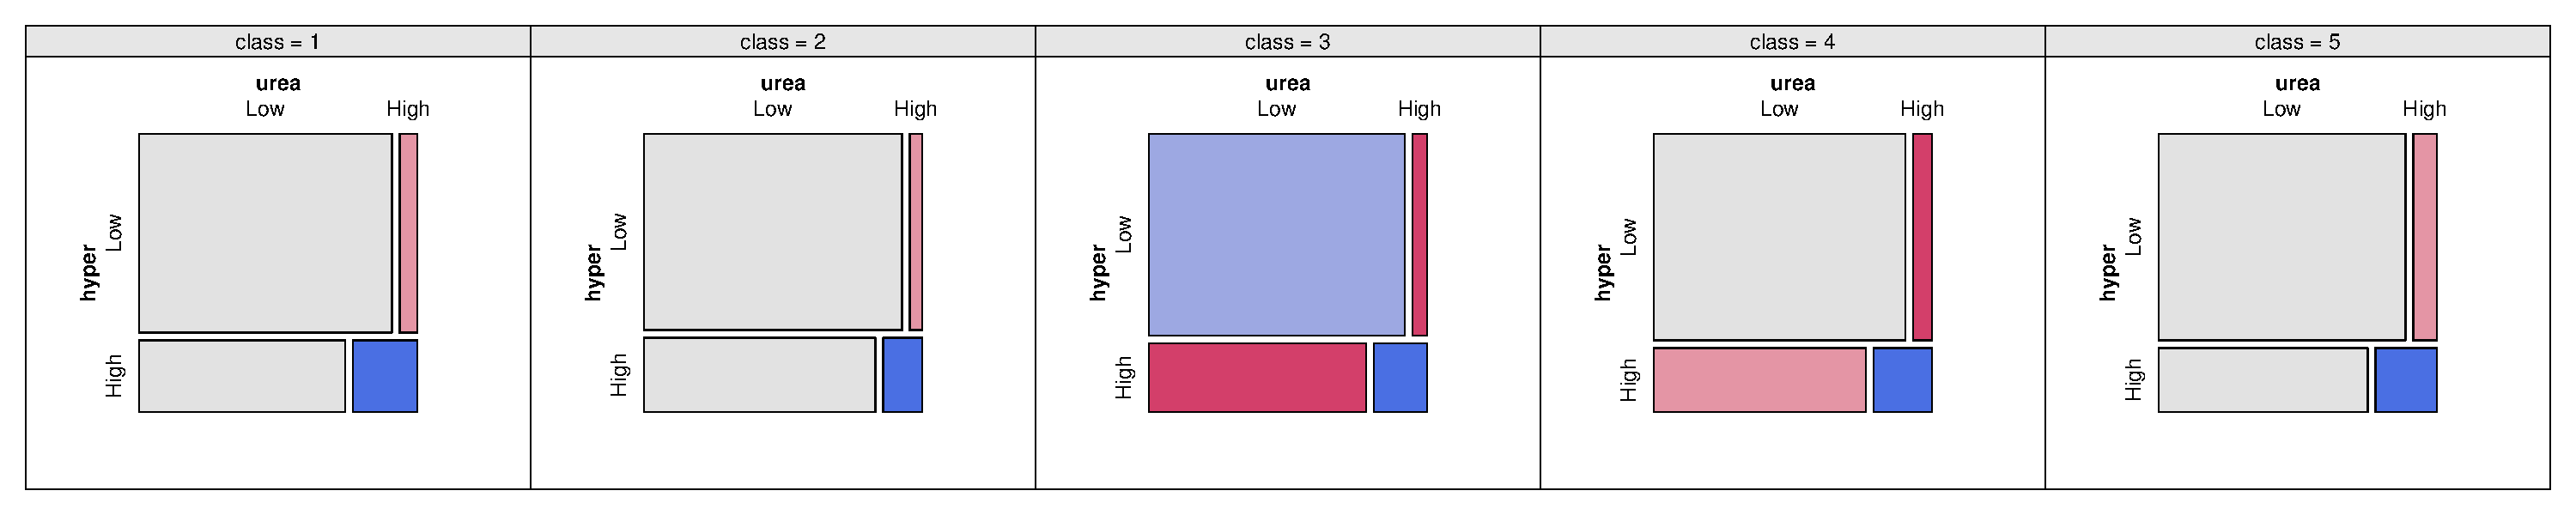
\includegraphics[width=1.1\textwidth]{ch08/fig/tox-mosaic3-1} }

\caption[Toxaemia data]{Toxaemia data: Response association conditioned on social class\label{fig:tox-mosaic3}}
\end{figure}


\end{knitrout}
Ignoring social class, the association between hypertension and protein urea
decreases with smoking.
Ignoring smoking, the association is greatest in social class 3.
However, these displays don't show directly how the two symptoms are
associated in the combinations of social class and smoking.
The fourfold display in \figref{fig:tox-fourfold}, does that.

% This generates huge figure margins, compressing the plot to a small area ...
% Need to use pdfcrop or crop manually...
%%%<<tox-fourfold, h=6, w=10, out.width='\\textwidth', cap='Fourfold display for Toxaemia data', crop=TRUE>>=
\begin{knitrout}
\definecolor{shadecolor}{rgb}{1, 0.961, 0.933}\color{fgcolor}\begin{kframe}
\begin{alltt}
\hlkwd{fourfold}\hlstd{(}\hlkwd{aperm}\hlstd{(tox.tab),} \hlkwc{fontsize}\hlstd{=}\hlnum{16}\hlstd{)}
\end{alltt}
\end{kframe}
\end{knitrout}
\begin{figure}[!htb]
\centering
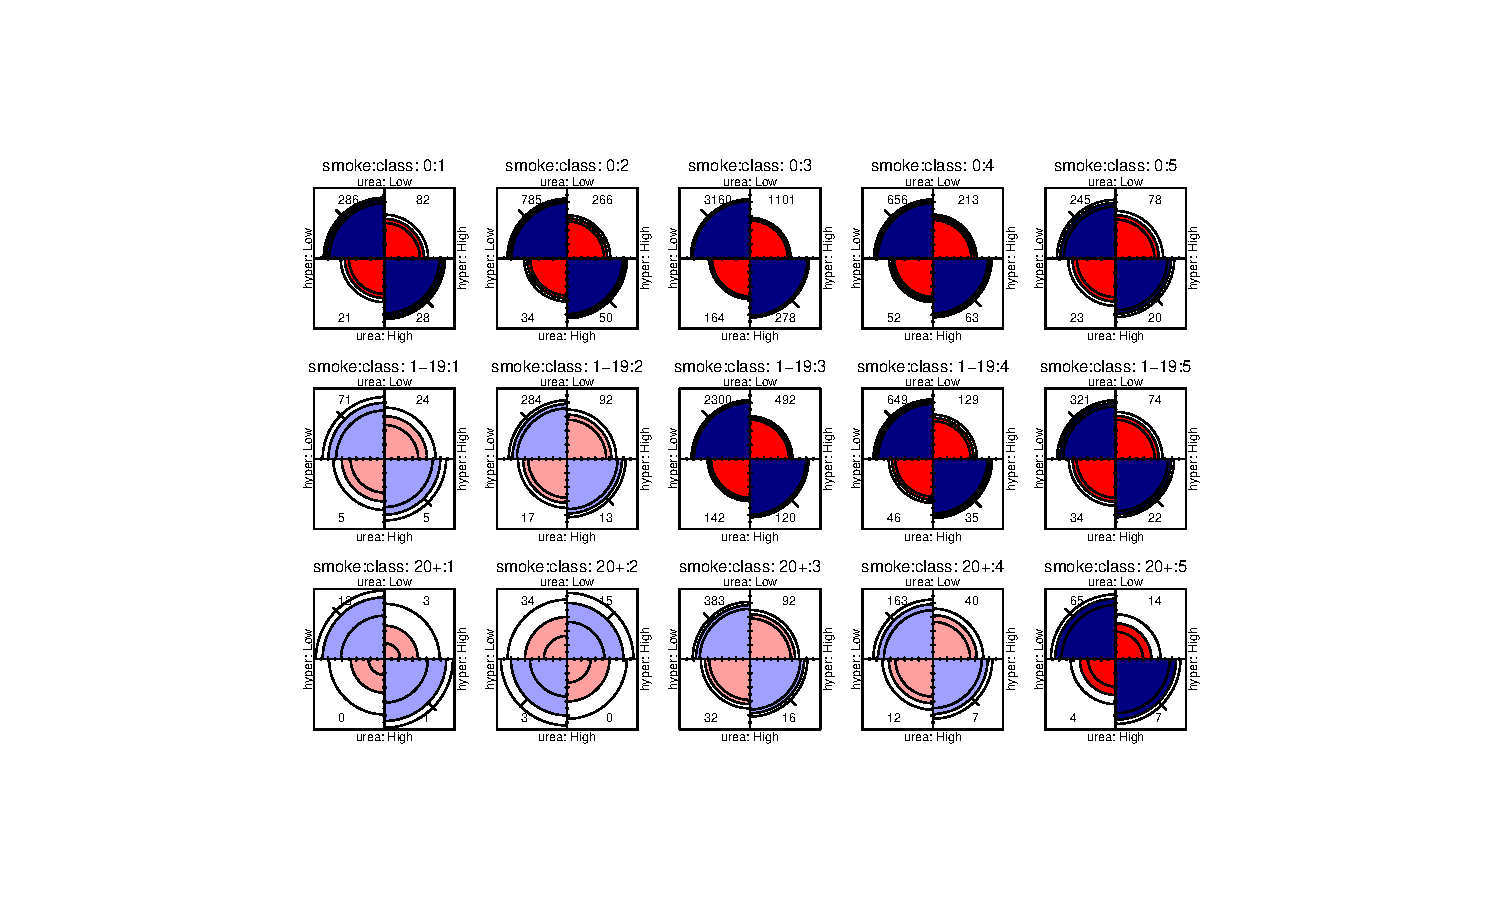
\includegraphics[width=.75\textwidth]{ch08/fig/tox-fourfold-crop}
\caption{Fourfold display for Toxaemia data. Smoking levels vary in the rows and social class in the columns.}
\label{fig:tox-fourfold}
\end{figure}

It can be seen in \figref{fig:tox-fourfold}
that the odds ratio appears to increase with both smoking and social class number and
these two symptoms are positively associated in nearly all cases.
In only two cases the odds ratio is not significantly different from 1:
mothers in classes 1 and 2, who smoke more than 20 cigarettes a day,
but the frequency in this cell is quite small.

\begin{knitrout}
\definecolor{shadecolor}{rgb}{1, 0.961, 0.933}\color{fgcolor}\begin{kframe}
\begin{alltt}
\hlkwd{t}\hlstd{(}\hlkwd{apply}\hlstd{(tox.tab,} \hlkwc{MARGIN}\hlstd{=}\hlnum{1}\hlopt{:}\hlnum{2}\hlstd{,} \hlkwc{FUN}\hlstd{=sum))}
\end{alltt}
\begin{verbatim}
##       class
## smoke    1    2    3   4   5
##   0    417 1135 4703 984 366
##   1-19 105  406 3054 859 451
##   20+   17   52  523 222  90
\end{verbatim}
\end{kframe}
\end{knitrout}

From these plots, it is useful to examine the association between hypertension
and urea more directly, by calculating and plotting the odds ratios.
For a $2 \times 2 \times K \times L \times \cdots$ table,
the function \func{oddsratio} in \pkg{vcd} calculates these for each $2 \times 2$
subtable, and returns an array of dimension $K \times L \times \cdots$,
together with similar array of standard errors.
\begin{knitrout}
\definecolor{shadecolor}{rgb}{1, 0.961, 0.933}\color{fgcolor}\begin{kframe}
\begin{alltt}
\hlstd{LOR} \hlkwb{<-}\hlkwd{oddsratio}\hlstd{(}\hlkwd{aperm}\hlstd{(tox.tab))}
\hlstd{LOR}
\end{alltt}
\begin{verbatim}
##           1        2      3       4      5
## 0    1.5370  1.46785 1.5821 1.31676 1.0048
## 1-19 1.0846  0.85892 1.3739 1.34233 1.0321
## 20+  2.4485 -1.14579 0.7331 0.86587 2.0949
\end{verbatim}
\end{kframe}
\end{knitrout}
The \func{plot} method for the resulting \class{logoddsratio} object only
handles a single stratum dimension, but in the present case
it is easy to plot the result
using \func{matplot} as we did earlier.  The lines below produce \figref{fig:tox-LOR}.

\begin{knitrout}
\definecolor{shadecolor}{rgb}{1, 0.961, 0.933}\color{fgcolor}\begin{kframe}
\begin{alltt}
\hlkwd{matplot}\hlstd{(}\hlkwd{t}\hlstd{(LOR),} \hlkwc{type}\hlstd{=}\hlstr{"b"}\hlstd{,}
        \hlkwc{cex}\hlstd{=}\hlnum{1.5}\hlstd{,} \hlkwc{pch}\hlstd{=}\hlnum{15}\hlopt{:}\hlnum{17}\hlstd{,} \hlkwc{cex.lab}\hlstd{=}\hlnum{1.5}\hlstd{,} \hlkwc{lwd}\hlstd{=}\hlnum{2}\hlstd{,} \hlkwc{lty}\hlstd{=}\hlnum{1}\hlstd{,}
        \hlkwc{ylab}\hlstd{=}\hlstr{'log odds ratio: Urea | Hypertension'}\hlstd{,}
        \hlkwc{xlab}\hlstd{=}\hlstr{'Social class of mother'}\hlstd{,}
        \hlkwc{xlim}\hlstd{=}\hlkwd{c}\hlstd{(}\hlnum{1}\hlstd{,}\hlnum{5.5}\hlstd{),} \hlkwc{col}\hlstd{=}\hlkwd{c}\hlstd{(}\hlstr{"blue"}\hlstd{,} \hlstr{"black"}\hlstd{,} \hlstr{"red"}\hlstd{)}
       \hlstd{)}
\hlkwd{abline}\hlstd{(}\hlkwc{h}\hlstd{=}\hlnum{0}\hlstd{,} \hlkwc{col}\hlstd{=}\hlstr{'gray'}\hlstd{)}
\hlkwd{text}\hlstd{(}\hlnum{5.2}\hlstd{, LOR[,}\hlnum{5}\hlstd{]}\hlopt{+}\hlkwd{c}\hlstd{(}\hlopt{-}\hlnum{.05}\hlstd{,}\hlnum{.05}\hlstd{,} \hlnum{0}\hlstd{),} \hlkwc{labels}\hlstd{=}\hlkwd{rownames}\hlstd{(LOR),} \hlkwc{cex}\hlstd{=}\hlnum{1.25}\hlstd{)}
\hlkwd{text}\hlstd{(}\hlnum{5.2}\hlstd{,} \hlkwd{max}\hlstd{(LOR[,}\hlnum{5}\hlstd{])}\hlopt{+}\hlnum{.2}\hlstd{,} \hlstr{"Smoking"}\hlstd{,} \hlkwc{cex}\hlstd{=}\hlnum{1.4}\hlstd{)}
\end{alltt}
\end{kframe}\begin{figure}[!htbp]


\centerline{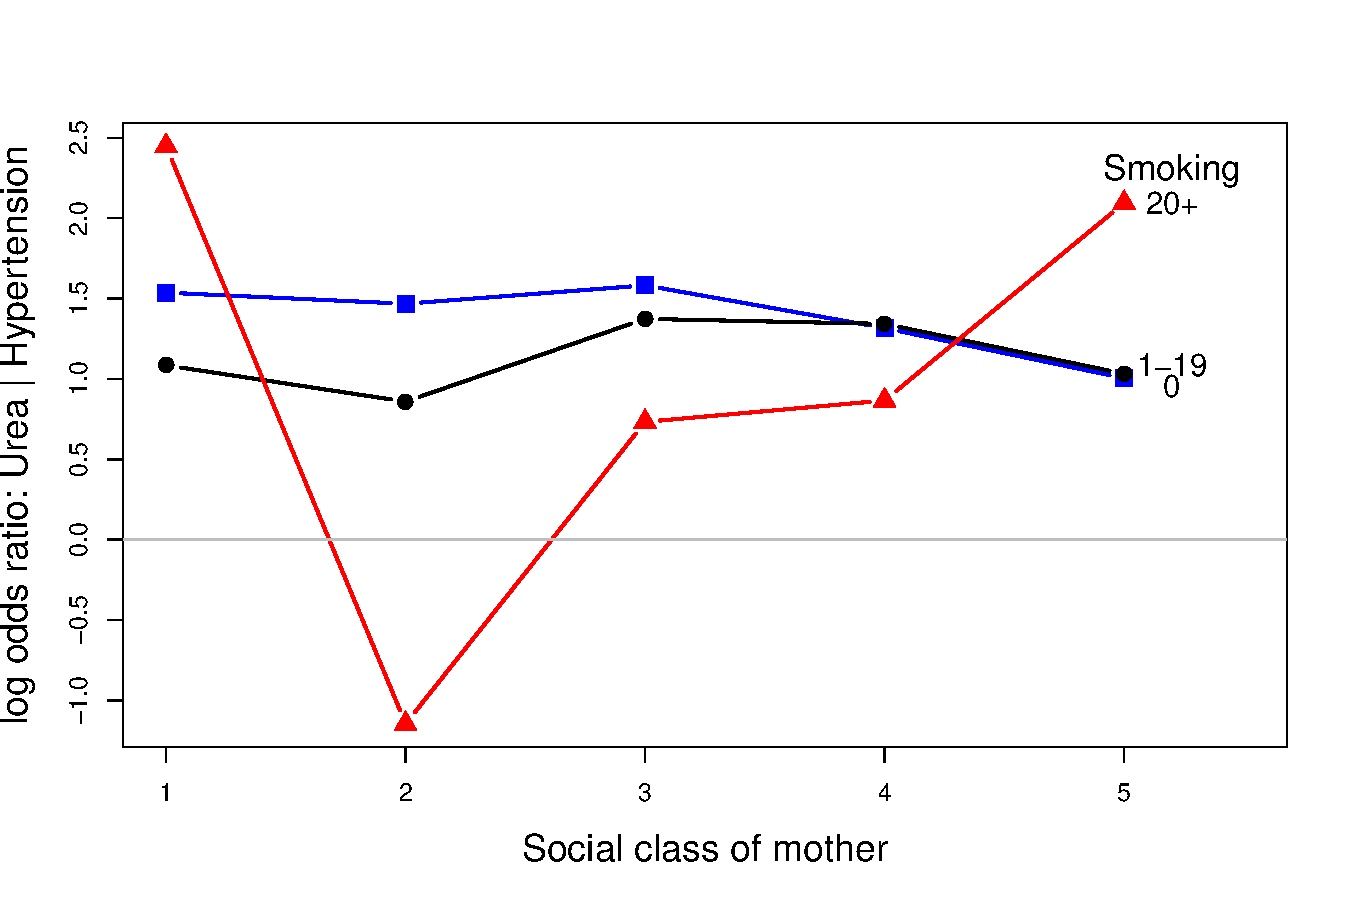
\includegraphics[width=.75\textwidth]{ch08/fig/tox-LOR-1} }

\caption[Log odds ratios for protein urea given hypertension, by social class and level of maternal smoking]{Log odds ratios for protein urea given hypertension, by social class and level of maternal smoking\label{fig:tox-LOR}}
\end{figure}


\end{knitrout}
The association between the response symptoms,
shown in \figref{fig:tox-LOR}
is clearer, once we take the variation in sample sizes into account.
Except for the heavy smokers, particularly  in social classes 1 and 2, the log odds ratio
appears to range only between 1--1.5, meaning that, given one symptom,
the odds of also having the other range between $\exp(1)=2.72$ and $\exp(1.5)=4.48$.

This initial overview of the data is completed
by calculating and plotting the log odds for each
symptom within each class-smoke population.
This could be done in the same way as in \exref{ex:coalminers},
(except that there are now two explanatory factors).
The steps used there were:
\begin{seriate}
 \item Reshape the $2 \times 2 \times K \cdots$ table to a matrix
 with four columns corresponding to the binary response combinations.
 \item Calculate the logits (and log odds ratio) using \func{blogits}.
\end{seriate}
\TODO{Use this as an exercise.}

Here, it is more useful to make separate plots for each of the logits,
and we illustrate a more general approach that applies to two or more
binary responses, with two or more predictor variables.
The essential idea is to fit a separate logit model for each response
separately, using the \emph{highest-order interaction} of all predictors
(the saturated model).  The fitted logits in these models then match
those in the data.
\begin{knitrout}
\definecolor{shadecolor}{rgb}{1, 0.961, 0.933}\color{fgcolor}\begin{kframe}
\begin{alltt}
\hlstd{tox.hyper} \hlkwb{<-} \hlkwd{glm}\hlstd{(hyper}\hlopt{==}\hlstr{'High'} \hlopt{~} \hlstd{class}\hlopt{*}\hlstd{smoke,} \hlkwc{weights}\hlstd{=Freq,}
                 \hlkwc{data}\hlstd{=Toxaemia,} \hlkwc{family}\hlstd{=binomial)}
\hlstd{tox.urea} \hlkwb{<-} \hlkwd{glm}\hlstd{(urea}\hlopt{==}\hlstr{'High'} \hlopt{~} \hlstd{class}\hlopt{*}\hlstd{smoke,} \hlkwc{weights}\hlstd{=Freq,}
                \hlkwc{data}\hlstd{=Toxaemia,} \hlkwc{family}\hlstd{=binomial)}
\end{alltt}
\end{kframe}
\end{knitrout}

It is then simple to plot these results using the \Rpackage{effects}
as shown in \figref{fig:tox-effplots}. Each plot shows the logit for
the response measure against class, with separate curves for the levels of smoking.%
\footnote{
As is usual for effect plots of binary response \func{glm} models, the vertical axis
is plotted on the scale of log odds, but labeled in terms of probabilities.
}

\begin{knitrout}
\definecolor{shadecolor}{rgb}{1, 0.961, 0.933}\color{fgcolor}\begin{kframe}
\begin{alltt}
\hlkwd{library}\hlstd{(effects)}

\hlkwd{plot}\hlstd{(}\hlkwd{allEffects}\hlstd{(tox.hyper),}
  \hlkwc{ylab} \hlstd{=} \hlstr{"Probability (hypertension)"}\hlstd{,}
  \hlkwc{xlab} \hlstd{=} \hlstr{"Social class of mother"}\hlstd{,}
  \hlkwc{main} \hlstd{=} \hlstr{"Hypertension: class*smoke effect plot"}\hlstd{,}
  \hlkwc{colors} \hlstd{=} \hlkwd{c}\hlstd{(}\hlstr{"blue"}\hlstd{,} \hlstr{"black"}\hlstd{,} \hlstr{"red"}\hlstd{),}
  \hlkwc{lwd}\hlstd{=}\hlnum{3}\hlstd{,}  \hlkwc{multiline}\hlstd{=}\hlnum{TRUE}\hlstd{,}
  \hlkwc{key.args}\hlstd{=}\hlkwd{list}\hlstd{(}\hlkwc{x}\hlstd{=}\hlnum{0.05}\hlstd{,} \hlkwc{y}\hlstd{=}\hlnum{0.2}\hlstd{,} \hlkwc{cex}\hlstd{=}\hlnum{1.2}\hlstd{)}
  \hlstd{)}

\hlkwd{plot}\hlstd{(}\hlkwd{allEffects}\hlstd{(tox.urea),}
  \hlkwc{ylab} \hlstd{=} \hlstr{"Probability (Urea)"}\hlstd{,}
  \hlkwc{xlab} \hlstd{=} \hlstr{"Social class of mother"}\hlstd{,}
  \hlkwc{main} \hlstd{=} \hlstr{"Urea: class*smoke effect plot"}\hlstd{,}
  \hlkwc{colors} \hlstd{=} \hlkwd{c}\hlstd{(}\hlstr{"blue"}\hlstd{,} \hlstr{"black"}\hlstd{,} \hlstr{"red"}\hlstd{),}
  \hlkwc{lwd}\hlstd{=}\hlnum{3}\hlstd{,}  \hlkwc{multiline}\hlstd{=}\hlnum{TRUE}\hlstd{,}
  \hlkwc{key.args}\hlstd{=}\hlkwd{list}\hlstd{(}\hlkwc{x}\hlstd{=}\hlnum{0.65}\hlstd{,} \hlkwc{y}\hlstd{=}\hlnum{0.2}\hlstd{,} \hlkwc{cex}\hlstd{=}\hlnum{1.2}\hlstd{)}
  \hlstd{)}
\end{alltt}
\end{kframe}\begin{figure}[!htbp]


\centerline{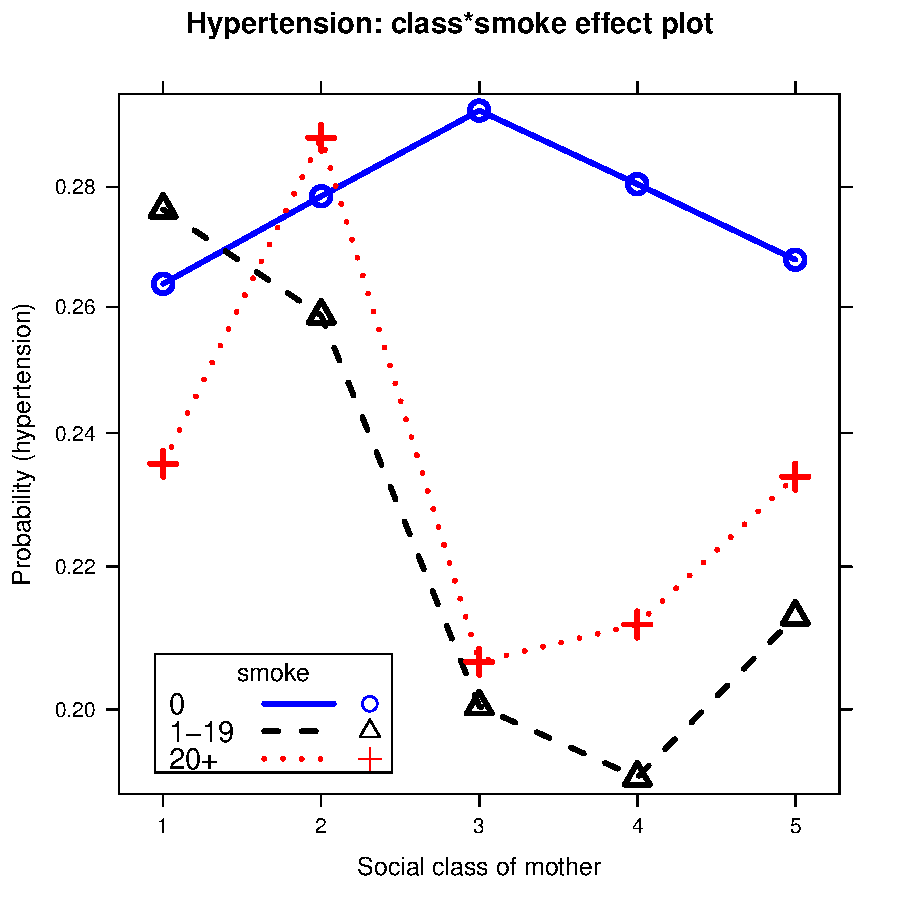
\includegraphics[width=.5\textwidth]{ch08/fig/tox-effplots-1} 
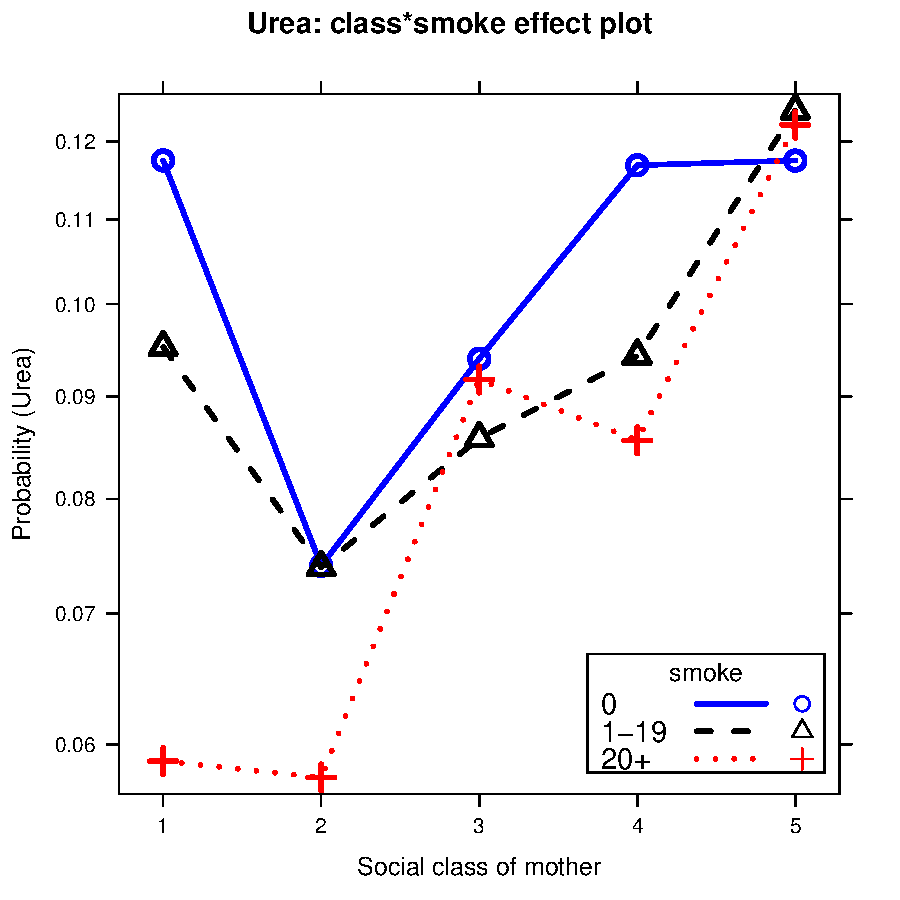
\includegraphics[width=.5\textwidth]{ch08/fig/tox-effplots-2} }

\caption[Plots of log odds for hypertension and urea, by social class of mother and smoking]{Plots of log odds for hypertension and urea, by social class of mother and smoking.\label{fig:tox-effplots}}
\end{figure}


\end{knitrout}
From \figref{fig:tox-effplots}, it can be seen that the prevalence of these
symptoms has a possibly complex relation to social class and smoking.
However, the mosaic for these predictors in \figref{fig:tox-mosaic1} has shown
us that several of the class-smoking categories are quite small
(particularly heavy smokers in Classes 1 and 2)
so the response effects for these classes will be poorly estimated.
Taking this into account,
we suspect that protein urea varies with social class, but not with
smoking, while the prevalence of hypertension may truly vary with neither,
just one, or both of these predictors.

\subsubsection*{Fitting models}

The plots shown so far in this example are all essentially \emph{data-based}, in that
they use the observed frequencies or transformations of them and don't
allow for a simpler view, based on a reasonable model.  That is,
abbreviating the table variables by their initial letters,
the plots in
\figref{fig:tox-LOR} and \figref{fig:tox-effplots} are plots of the
saturated model, \LLM{CSHU} that fits perfectly, but with the data transformed
for each $2 \times 2$ subtable to the log odds ratio and the two log odds
for \code{hyper} and \code{urea}.

The bivariate logistic model fit by \func{vglm} still applies when there are
two or more predictors; however, like other multivariate response models, it
doesn't easily allow the logits to depend on \emph{different} predictor terms.
To illustrate this, we first transform the \data{Toxaemia} to a
$15 \times 4$ data frame in the form required by \func{vglm}.

\begin{knitrout}
\definecolor{shadecolor}{rgb}{1, 0.961, 0.933}\color{fgcolor}\begin{kframe}
\begin{alltt}
\hlstd{tox.tab} \hlkwb{<-} \hlkwd{xtabs}\hlstd{(Freq}\hlopt{~}\hlstd{class} \hlopt{+} \hlstd{smoke} \hlopt{+} \hlstd{hyper} \hlopt{+} \hlstd{urea, Toxaemia)}
\hlstd{toxaemia} \hlkwb{<-} \hlkwd{t}\hlstd{(}\hlkwd{matrix}\hlstd{(}\hlkwd{aperm}\hlstd{(tox.tab),} \hlnum{4}\hlstd{,} \hlnum{15}\hlstd{))}
\hlkwd{colnames}\hlstd{(toxaemia)} \hlkwb{<-} \hlkwd{c}\hlstd{(}\hlstr{"hu"}\hlstd{,} \hlstr{"hU"}\hlstd{,} \hlstr{"Hu"}\hlstd{,} \hlstr{"HU"}\hlstd{)}
\hlstd{rowlabs} \hlkwb{<-} \hlkwd{expand.grid}\hlstd{(}\hlkwc{smoke}\hlstd{=}\hlkwd{c}\hlstd{(}\hlstr{"0"}\hlstd{,} \hlstr{"1-19"}\hlstd{,} \hlstr{"20+"}\hlstd{),} \hlkwc{class}\hlstd{=}\hlkwd{factor}\hlstd{(}\hlnum{1}\hlopt{:}\hlnum{5}\hlstd{))}
\hlstd{toxaemia} \hlkwb{<-} \hlkwd{cbind}\hlstd{(toxaemia, rowlabs)}
\hlkwd{head}\hlstd{(toxaemia)}
\end{alltt}
\begin{verbatim}
##    hu hU  Hu HU smoke class
## 1 286 21  82 28     0     1
## 2  71  5  24  5  1-19     1
## 3  13  0   3  1   20+     1
## 4 785 34 266 50     0     2
## 5 284 17  92 13  1-19     2
## 6  34  3  15  0   20+     2
\end{verbatim}
\end{kframe}
\end{knitrout}
In the model specification for \func{vglm}, the \code{zero} argument in
\func{binom.or} allows any one or more of the two log odds and log odds
ratio to be fit as a constant (intercept-only) in \eqref{eq:blogits2}.
However, in that equation, the predictors $\vec{x}_1$, $\vec{x}_2$, $\vec{x}_{12}$,
must be the \emph{same} in all three submodels.  For example, the model
\code{tox.vglm1} below uses main effects of \code{class} and \code{smoke}
in both models for the logits, and \code{zero=3} for a constant
log odds ratio.
\begin{knitrout}
\definecolor{shadecolor}{rgb}{1, 0.961, 0.933}\color{fgcolor}\begin{kframe}
\begin{alltt}
\hlstd{tox.vglm1} \hlkwb{<-} \hlkwd{vglm}\hlstd{(}\hlkwd{cbind}\hlstd{(hu, hU, Hu, Hu)} \hlopt{~} \hlstd{class} \hlopt{+} \hlstd{smoke,}
                  \hlkwd{binom2.or}\hlstd{(}\hlkwc{zero}\hlstd{=}\hlnum{3}\hlstd{),} \hlkwc{data}\hlstd{=toxaemia)}
\hlkwd{coef}\hlstd{(tox.vglm1,} \hlkwc{matrix}\hlstd{=}\hlnum{TRUE}\hlstd{)}
\end{alltt}
\begin{verbatim}
##              logit(mu1) logit(mu2) log(oratio)
## (Intercept) -0.50853648 -1.2214518      2.7808
## class2       0.18156457  0.0382046      0.0000
## class3       0.06332765 -0.0087552      0.0000
## class4      -0.02227055 -0.0031541      0.0000
## class5      -0.00077172  0.0821863      0.0000
## smoke1-19   -0.41298650 -0.2198673      0.0000
## smoke20+    -0.30562472 -0.1245019      0.0000
\end{verbatim}
\end{kframe}
\end{knitrout}

Instead, when there are no quantitative predictors, and when the odds ratio is
relatively constant (as here)
it is easier to fit ordinary \loglin models
than to use the bivariate logit formulation of the previous example.
These allow the responses $H$ and $U$ to depend on the class-smoking
combinations separately, by including the terms $[CSH]$ or $[CSU]$,
respectively.

The minimal, null model, $[CS] [H] [U]$ fits the marginal association of the
numbers in each class-smoking category, but asserts that the responses,
$H$ and $U$ are independent, which we have already seen is contradicted
by the data.  We take $[CS] [HU]$ as the baseline model (Model 1), asserting no relation
between response and predictor variables, but associations within each set are allowed,
These models are fit as shown below.
\begin{knitrout}
\definecolor{shadecolor}{rgb}{1, 0.961, 0.933}\color{fgcolor}\begin{kframe}
\begin{alltt}
\hlcom{# null model}
\hlstd{tox.glm0} \hlkwb{<-} \hlkwd{glm}\hlstd{(Freq} \hlopt{~} \hlstd{class}\hlopt{*}\hlstd{smoke} \hlopt{+} \hlstd{hyper} \hlopt{+} \hlstd{urea,}
                \hlkwc{data}\hlstd{=Toxaemia,} \hlkwc{family}\hlstd{=poisson)}
\hlcom{# baseline model: no association between predictors and responses}
\hlstd{tox.glm1} \hlkwb{<-} \hlkwd{glm}\hlstd{(Freq} \hlopt{~} \hlstd{class}\hlopt{*}\hlstd{smoke} \hlopt{+} \hlstd{hyper}\hlopt{*}\hlstd{urea,}
                \hlkwc{data}\hlstd{=Toxaemia,} \hlkwc{family}\hlstd{=poisson)}
\end{alltt}
\end{kframe}
\end{knitrout}

We proceed to fit a collection of other models, adding terms to allow more associations
between the responses and predictors. Summary measures of goodness of fit
and parsimony are shown in \tabref{tab:toxmod}.
\begin{table}[htb]
 \caption{Loglinear models, \code{tox.glm*}, fit to the Toxaemia data}\label{tab:toxmod}
 \begin{center}
 \begin{tabular}{rl rrrrrrr}
  \hline
  Model & Terms         & df & \GSQ & $p$-value & \GSQ /df & AIC & BIC & $R^2$  \\ 
  \hline
  0 & CS H U            & 43 & 672.85 & 0.0000 & 15.65 & 586.85 &  264.27 & .      \\ 
  1 & CS HU             & 42 & 179.03 & 0.0000 & 4.26  &  95.03 & -220.04 & 0.000  \\ 
  2 & CS HU SH CU       & 36 & 46.12  & 0.1203 & 1.28  & -25.88 & -295.94 & 0.742  \\ 
  3 & CS CH CU HU SH CU & 30 & 40.47  & 0.0960 & 1.35  & -19.53 & -244.58 & 0.774  \\ 
  4 & CSH CU HU         & 24 & 26.00  & 0.3529 & 1.08  & -22.00 & -202.04 & 0.855  \\ 
  5 & CSH CU SU HU      & 22 & 25.84  & 0.2588 & 1.17  & -18.16 & -183.20 & 0.856  \\ 
  6 & CSH CSU HU        & 14 & 22.29  & 0.0729 & 1.59  & -5.71  & -110.74 & 0.875  \\ 
  7 & CSH CSU SHU       & 12 & 15.65  & 0.2079 & 1.30  & -8.35  &  -98.37 & 0.913  \\ 
  8 & CSH CSU CHU SHU   & 8  & 12.68  & 0.1233 & 1.59  & -3.32  &  -63.33 & 0.929  \\ 
  9 & CSHU              & 0  & 0.00   & 0      & 0     &  0.00  &    0.00 & 1.000  \\ 
  \hline
 \end{tabular}
 \end{center}
\end{table}

\endinput

%> summarise(mods)
%Model Summary:
%         LR Chisq Df Pr(>Chisq)    AIC      BIC
%tox.glm0   672.85 43    0.00000 586.85  264.272
%tox.glm1   179.03 42    0.00000  95.03 -220.044
%tox.glm2    46.12 36    0.12030 -25.88 -295.943
%tox.glm3    40.47 30    0.09603 -19.53 -244.582
%tox.glm4    26.00 24    0.35294 -22.00 -202.039
%tox.glm5    25.84 22    0.25875 -18.16 -183.203
%tox.glm6    22.29 14    0.07293  -5.71 -110.740
%tox.glm7    15.65 12    0.20789  -8.35  -98.374
%tox.glm8    12.68  8    0.12332  -3.32  -63.334
%tox.glm9     0.00  0    0.00000   0.00    0.000
%> 
%
%> aic <- AIC(tox.glm0, tox.glm1, tox.glm2, tox.glm3, 
%+            tox.glm4, tox.glm5, tox.glm6, tox.glm7, tox.glm8, tox.glm9)
%> bic <- BIC(tox.glm0, tox.glm1, tox.glm2, tox.glm3, 
%+            tox.glm4, tox.glm5, tox.glm6, tox.glm7, tox.glm8, tox.glm9)
%> merge(aic,bic, by=c(0,1))
%   Row.names df       AIC       BIC
%1   tox.glm0 17 1048.3057 1083.9095
%2   tox.glm1 18  556.4877  594.1859
%3   tox.glm2 24  435.5779  485.8422
%4   tox.glm3 30  441.9280  504.7583
%5   tox.glm4 36  439.4600  514.8564
%6   tox.glm5 38  443.2925  522.8776
%7   tox.glm6 46  455.7412  552.0810
%8   tox.glm7 48  453.1037  553.6322
%9   tox.glm8 52  458.1364  567.0423
%10  tox.glm9 60  461.4556  587.1163
%> 
%



\begin{knitrout}\footnotesize
\definecolor{shadecolor}{rgb}{1, 0.961, 0.933}\color{fgcolor}\begin{kframe}
\begin{alltt}
\hlstd{tox.glm2} \hlkwb{<-} \hlkwd{update}\hlstd{(tox.glm1, .} \hlopt{~} \hlstd{.} \hlopt{+} \hlstd{smoke}\hlopt{*}\hlstd{hyper} \hlopt{+} \hlstd{class}\hlopt{*}\hlstd{urea)}

\hlstd{tox.glm3} \hlkwb{<-} \hlkwd{glm}\hlstd{(Freq} \hlopt{~} \hlstd{(class} \hlopt{+} \hlstd{smoke} \hlopt{+} \hlstd{hyper} \hlopt{+} \hlstd{urea)}\hlopt{^}\hlnum{2}\hlstd{,}
                \hlkwc{data}\hlstd{=Toxaemia,} \hlkwc{family}\hlstd{=poisson)}

\hlstd{tox.glm4} \hlkwb{<-} \hlkwd{glm}\hlstd{(Freq} \hlopt{~} \hlstd{class}\hlopt{*}\hlstd{smoke}\hlopt{*}\hlstd{hyper} \hlopt{+} \hlstd{hyper}\hlopt{*}\hlstd{urea} \hlopt{+} \hlstd{class}\hlopt{*}\hlstd{urea,}
                \hlkwc{data}\hlstd{=Toxaemia,} \hlkwc{family}\hlstd{=poisson)}

\hlstd{tox.glm5} \hlkwb{<-} \hlkwd{update}\hlstd{(tox.glm4, .} \hlopt{~} \hlstd{.} \hlopt{+} \hlstd{smoke}\hlopt{*}\hlstd{urea)}

\hlstd{tox.glm6} \hlkwb{<-} \hlkwd{update}\hlstd{(tox.glm4, .} \hlopt{~} \hlstd{.} \hlopt{+} \hlstd{class}\hlopt{*}\hlstd{smoke}\hlopt{*}\hlstd{urea)}

\hlstd{tox.glm7} \hlkwb{<-} \hlkwd{update}\hlstd{(tox.glm6, .} \hlopt{~} \hlstd{.} \hlopt{+} \hlstd{smoke}\hlopt{*}\hlstd{hyper}\hlopt{*}\hlstd{urea)}

\hlstd{tox.glm8} \hlkwb{<-} \hlkwd{glm}\hlstd{(Freq} \hlopt{~} \hlstd{(class} \hlopt{+} \hlstd{smoke} \hlopt{+} \hlstd{hyper} \hlopt{+} \hlstd{urea)}\hlopt{^}\hlnum{3}\hlstd{,}
                \hlkwc{data}\hlstd{=Toxaemia,} \hlkwc{family}\hlstd{=poisson)}

\hlstd{tox.glm9} \hlkwb{<-} \hlkwd{glm}\hlstd{(Freq} \hlopt{~} \hlstd{(class} \hlopt{+} \hlstd{smoke} \hlopt{+} \hlstd{hyper} \hlopt{+} \hlstd{urea)}\hlopt{^}\hlnum{4}\hlstd{,}
                \hlkwc{data}\hlstd{=Toxaemia,} \hlkwc{family}\hlstd{=poisson)}
\end{alltt}
\end{kframe}
\end{knitrout}

Model 2 adds the simple dependence of hypertension on smoking ($[SH]$)
and that of urea on class ($[CU]$).
Model 3 includes all two-way terms.
In Model 4, hypertension is allowed to depend on both class and smoking
jointly ($[CSH]$). In Model 5 an additional dependence of
urea on smoking ($[SU]$) is included, while in Model 6 urea depends on
class and smoking jointly ($[CSU]$).

None of these models contain three-way terms involving both $H$ and $U$,
so these models assume that the log odds ratio for hypertension given urea
is constant over the explanatory variables.
Recalling the conditional mosaics (\figref{fig:tox-mosaic2} and \figref{fig:tox-mosaic3}),
Models 7 and 8 add terms
which allow the odds ratio to vary, first with smoking ($[SHU]$), then
with class ($[CHU]$) as well.
Finally, Model 9 is the saturated model, that fits perfectly.

How do we choose among these models?  Model 2 is the smallest model whose deviance
is non-significant.
Models 4 and 5 both have a smaller ratio of \GSQ /df.
For comparing nested models, we can also examine the change in deviance as
terms are added (or dropped).  Thus, going from Model 2 to Model 3
decreases the deviance by 5.65 on 6 df,
while the step from Model 3 to Model 4
gives a decrease of 14.47, also on 6 df.
These tests can be performed using \func{lrtest} in the \Rpackage{lmtest},
shown below for models \code{tox.glm1}--\code{tox.glm5}.
\begin{knitrout}\footnotesize
\definecolor{shadecolor}{rgb}{1, 0.961, 0.933}\color{fgcolor}\begin{kframe}
\begin{alltt}
\hlkwd{library}\hlstd{(lmtest)}
\hlstd{lmtest::}\hlkwd{lrtest}\hlstd{(tox.glm1, tox.glm2, tox.glm3, tox.glm4, tox.glm5)}
\end{alltt}
\begin{verbatim}
## Likelihood ratio test
## 
## Model 1: Freq ~ class * smoke + hyper * urea
## Model 2: Freq ~ class + smoke + hyper + urea + class:smoke + hyper:urea + 
##     smoke:hyper + class:urea
## Model 3: Freq ~ (class + smoke + hyper + urea)^2
## Model 4: Freq ~ class * smoke * hyper + hyper * urea + class * urea
## Model 5: Freq ~ class + smoke + hyper + urea + class:smoke + class:hyper + 
##     smoke:hyper + hyper:urea + class:urea + smoke:urea + class:smoke:hyper
##   #Df LogLik Df  Chisq Pr(>Chisq)    
## 1  18   -260                         
## 2  24   -194  6 132.91     <2e-16 ***
## 3  30   -191  6   5.65      0.464    
## 4  36   -184  6  14.47      0.025 *  
## 5  38   -184  2   0.17      0.920    
## ---
## Signif. codes:  0 '***' 0.001 '**' 0.01 '*' 0.05 '.' 0.1 ' ' 1
\end{verbatim}
\end{kframe}
\end{knitrout}
\noindent
The AIC  and BIC statistics, balancing
parsimony and goodness-of-fit, have their minimum value for Model 2,
which we adopt here for this example.

\subsubsection*{Plotting model results}
Whatever model is chosen, as a final step, it is important to determine what
that model implies about the original research questions.
Because our focus here is on the prevalence of each symptom, and their
association, it is helpful to graph the fitted logits and log odds ratios
implied by the model, as was done in \figref{fig:cm-vglm1} and \figref{fig:cm-vglm2-blogit}.

The presentation goal here is to produce plots showing the
observed logits and log odds ratios as in \figref{fig:tox-effplots} and \figref{fig:tox-LOR},
supplemented by lines showing these values according to the fitted model.
In \exref{ex:coalminers} we fit the bivariate logit model, for which the
response functions were the desired logits and log odds.
Here, where we have fit ordinary \loglin models, the observed and
fitted logits can be calculated from the observed and fitted frequencies.
The calculations require a bit of \R calisthenics to arrange these
into forms suitable for plotting.

As we did earlier, we first reshape the \data{Toxemia} to wide format,
as a $15 \times 4$ table of observed frequencies.
Because there are now two predictor variables, we take care to
include the levels of \code{smoke} and \code{class} as additional columns.
\begin{knitrout}
\definecolor{shadecolor}{rgb}{1, 0.961, 0.933}\color{fgcolor}\begin{kframe}
\begin{alltt}
\hlcom{# reshape to 15 x 4 table of frequencies}
\hlstd{tox.tab} \hlkwb{<-} \hlkwd{xtabs}\hlstd{(Freq}\hlopt{~}\hlstd{class} \hlopt{+} \hlstd{smoke} \hlopt{+} \hlstd{hyper} \hlopt{+} \hlstd{urea, Toxaemia)}
\hlstd{toxaemia} \hlkwb{<-} \hlkwd{t}\hlstd{(}\hlkwd{matrix}\hlstd{(}\hlkwd{aperm}\hlstd{(tox.tab),} \hlnum{4}\hlstd{,} \hlnum{15}\hlstd{))}
\hlkwd{colnames}\hlstd{(toxaemia)} \hlkwb{<-} \hlkwd{c}\hlstd{(}\hlstr{"hu"}\hlstd{,} \hlstr{"hU"}\hlstd{,} \hlstr{"Hu"}\hlstd{,} \hlstr{"HU"}\hlstd{)}
\hlstd{rowlabs} \hlkwb{<-} \hlkwd{expand.grid}\hlstd{(}\hlkwc{smoke}\hlstd{=}\hlkwd{c}\hlstd{(}\hlstr{"0"}\hlstd{,} \hlstr{"1-19"}\hlstd{,} \hlstr{"20+"}\hlstd{),} \hlkwc{class}\hlstd{=}\hlkwd{factor}\hlstd{(}\hlnum{1}\hlopt{:}\hlnum{5}\hlstd{))}
\hlstd{toxaemia} \hlkwb{<-} \hlkwd{cbind}\hlstd{(toxaemia, rowlabs)}
\end{alltt}
\end{kframe}
\end{knitrout}
Applying \func{blogits}, we get the observed logits and log odds ratios
in \code{logitsTox}.
\begin{knitrout}
\definecolor{shadecolor}{rgb}{1, 0.961, 0.933}\color{fgcolor}\begin{kframe}
\begin{alltt}
\hlcom{# observed logits and log odds ratios}
\hlstd{logitsTox} \hlkwb{<-} \hlkwd{blogits}\hlstd{(toxaemia[,}\hlnum{4}\hlopt{:}\hlnum{1}\hlstd{],} \hlkwc{add}\hlstd{=}\hlnum{0.5}\hlstd{)}
\hlkwd{colnames}\hlstd{(logitsTox)[}\hlnum{1}\hlopt{:}\hlnum{2}\hlstd{]} \hlkwb{<-} \hlkwd{c}\hlstd{(}\hlstr{"logitH"}\hlstd{,} \hlstr{"logitU"}\hlstd{)}
\hlstd{logitsTox} \hlkwb{<-} \hlkwd{cbind}\hlstd{(logitsTox, rowlabs)}
\hlkwd{head}\hlstd{(logitsTox)}
\end{alltt}
\begin{verbatim}
##     logitH  logitU    logOR smoke class
## 1 -1.02057 -1.9988  1.52679     0     1
## 2 -0.94261 -2.1665  1.07102  1-19     1
## 3 -1.02962 -2.1401  2.44854   20+     1
## 4 -0.95040 -2.5158  1.46196     0     2
## 5 -1.04699 -2.4983  0.86401  1-19     2
## 6 -0.86500 -2.5257 -1.14579   20+     2
\end{verbatim}
\end{kframe}
\end{knitrout}

The fitted frequencies are extracted using \code{predict(tox.glm2, type="response")}
and then manipulated in a similar way to give \code{logitsFit}.
\begin{knitrout}
\definecolor{shadecolor}{rgb}{1, 0.961, 0.933}\color{fgcolor}\begin{kframe}
\begin{alltt}
\hlcom{# fitted frequencies, as a 15 x 4 table}
\hlstd{Fit} \hlkwb{<-} \hlkwd{t}\hlstd{(}\hlkwd{matrix}\hlstd{(}\hlkwd{predict}\hlstd{(tox.glm2,} \hlkwc{type}\hlstd{=}\hlstr{"response"}\hlstd{),} \hlnum{4}\hlstd{,} \hlnum{15}\hlstd{))}
\hlkwd{colnames}\hlstd{(Fit)} \hlkwb{<-} \hlkwd{c}\hlstd{(}\hlstr{"HU"}\hlstd{,} \hlstr{"Hu"}\hlstd{,} \hlstr{"hU"}\hlstd{,} \hlstr{"hu"}\hlstd{)}
\hlstd{Fit} \hlkwb{<-} \hlkwd{cbind}\hlstd{(Fit, rowlabs)}
\hlstd{logitsFit} \hlkwb{<-} \hlkwd{blogits}\hlstd{(Fit[,}\hlnum{1}\hlopt{:}\hlnum{4}\hlstd{],} \hlkwc{add}\hlstd{=}\hlnum{0.5}\hlstd{)}
\hlkwd{colnames}\hlstd{(logitsFit)[}\hlnum{1}\hlopt{:}\hlnum{2}\hlstd{]} \hlkwb{<-} \hlkwd{c}\hlstd{(}\hlstr{"logitH"}\hlstd{,} \hlstr{"logitU"}\hlstd{)}
\hlstd{logitsFit} \hlkwb{<-} \hlkwd{cbind}\hlstd{(logitsFit, rowlabs)}
\end{alltt}
\end{kframe}
\end{knitrout}
In tabular form, you can examine any of these components, for example,
the log odds ratios from the fitted values shown below.
\begin{knitrout}
\definecolor{shadecolor}{rgb}{1, 0.961, 0.933}\color{fgcolor}\begin{kframe}
\begin{alltt}
\hlkwd{matrix}\hlstd{(logitsFit}\hlopt{$}\hlstd{logOR,} \hlnum{3}\hlstd{,} \hlnum{5}\hlstd{,}
       \hlkwc{dimnames}\hlstd{=}\hlkwd{list}\hlstd{(}\hlkwc{smoke}\hlstd{=}\hlkwd{c}\hlstd{(}\hlstr{"0"}\hlstd{,} \hlstr{"1-19"}\hlstd{,} \hlstr{"20+"}\hlstd{),} \hlkwc{class}\hlstd{=}\hlnum{1}\hlopt{:}\hlnum{5}\hlstd{))}
\end{alltt}
\begin{verbatim}
##       class
## smoke       1      2      3      4      5
##   0    1.3588 1.3638 1.3675 1.3643 1.3582
##   1-19 1.3582 1.3678 1.3683 1.3674 1.3658
##   20+  1.2799 1.3471 1.3662 1.3622 1.3511
\end{verbatim}
\end{kframe}
\end{knitrout}

\begin{figure}
\centering
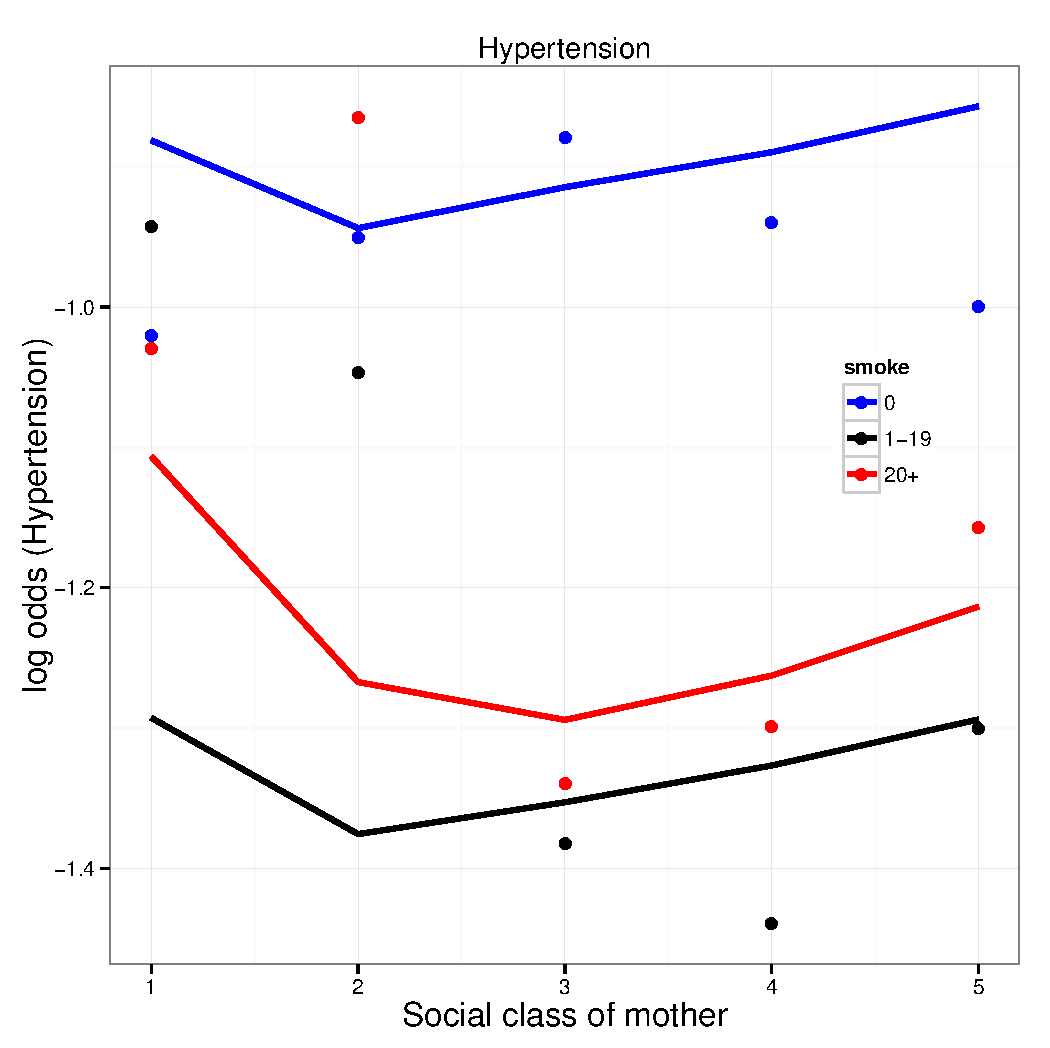
\includegraphics[width=.49\textwidth]{ch08/fig/tox-glm-logits1}
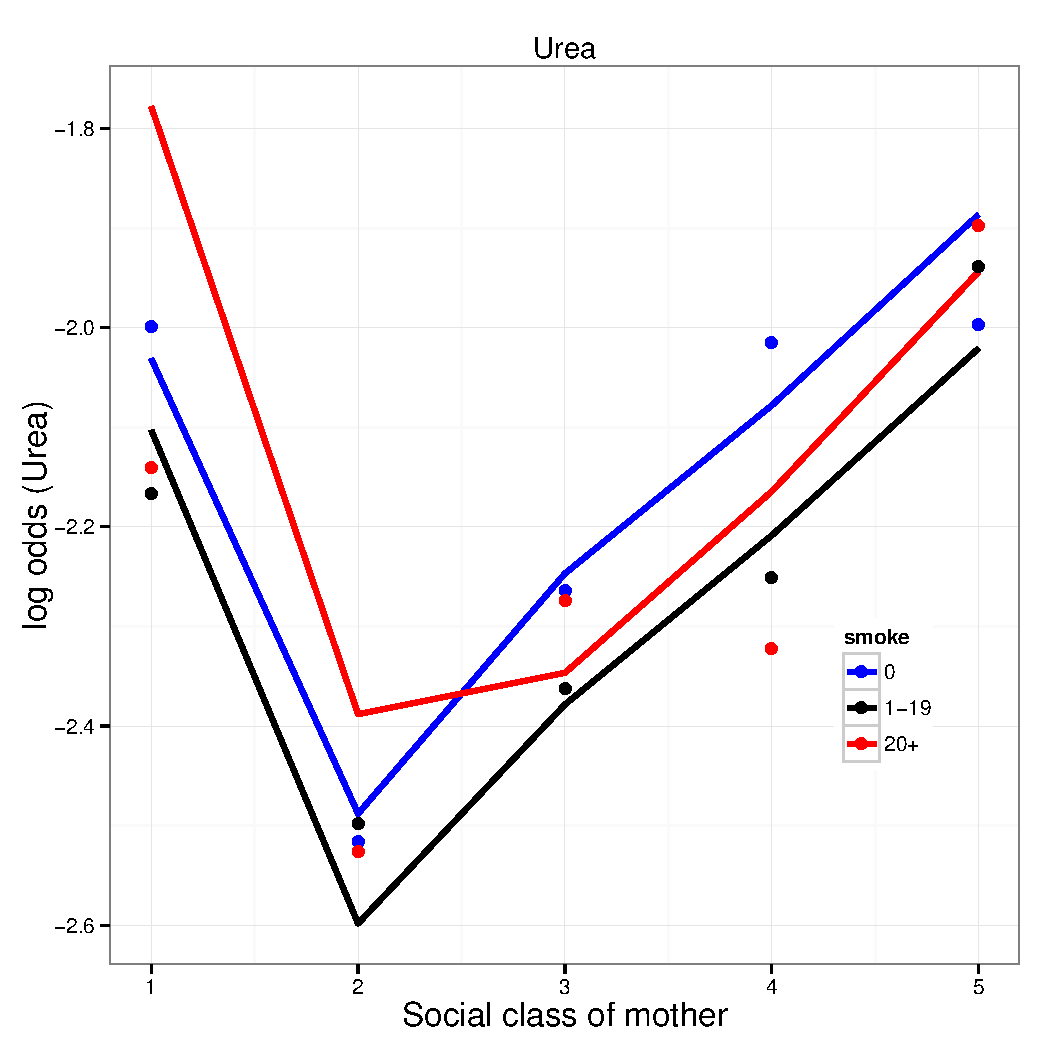
\includegraphics[width=.49\textwidth]{ch08/fig/tox-glm-logits2}
\caption{Observed (points) and fitted (lines) logits for the \data{Toxemia} data under Model 2.}
\label{fig:tox-glm-logits1}
\end{figure}

Finally, we can plot the observed values in \code{logitsTox} (as points) and the
fitted values under Model 2 in \code{logitsFit} (as lines),
separately for the \code{logitH}, \code{logitU}, and \code{logOR} components.
The code below uses \pkg{ggplot2} for the log odds of hypertension,
and is repeated for urea and the log odds ratio.
These graphs are shown in \figref{fig:tox-glm-logits1} and \figref{fig:tox-glm-logits3}.
\begin{knitrout}
\definecolor{shadecolor}{rgb}{1, 0.961, 0.933}\color{fgcolor}\begin{kframe}
\begin{alltt}
\hlkwd{ggplot}\hlstd{(logitsFit,} \hlkwd{aes}\hlstd{(}\hlkwc{x}\hlstd{=}\hlkwd{as.numeric}\hlstd{(class),} \hlkwc{y}\hlstd{=logitH,} \hlkwc{color}\hlstd{=smoke))} \hlopt{+}
  \hlkwd{theme_bw}\hlstd{()} \hlopt{+}
  \hlkwd{geom_line}\hlstd{(}\hlkwc{size}\hlstd{=}\hlnum{1.2}\hlstd{)} \hlopt{+}
  \hlkwd{scale_color_manual}\hlstd{(}\hlkwc{values}\hlstd{=}\hlkwd{c}\hlstd{(}\hlstr{"blue"}\hlstd{,} \hlstr{"black"}\hlstd{,} \hlstr{"red"}\hlstd{))} \hlopt{+}
  \hlkwd{ylab}\hlstd{(}\hlstr{"log odds (Hypertension)"}\hlstd{)} \hlopt{+}
  \hlkwd{xlab}\hlstd{(}\hlstr{"Social class of mother"}\hlstd{)} \hlopt{+}
  \hlkwd{ggtitle}\hlstd{(}\hlstr{"Hypertension"}\hlstd{)} \hlopt{+}
  \hlkwd{theme}\hlstd{(}\hlkwc{axis.title}\hlstd{=}\hlkwd{element_text}\hlstd{(}\hlkwc{size}\hlstd{=}\hlnum{16}\hlstd{))} \hlopt{+}
  \hlkwd{geom_point}\hlstd{(}\hlkwc{data}\hlstd{=logitsTox,}
             \hlkwd{aes}\hlstd{(}\hlkwc{x}\hlstd{=}\hlkwd{as.numeric}\hlstd{(class),} \hlkwc{y}\hlstd{=logitH,} \hlkwc{color}\hlstd{=smoke),} \hlkwc{size}\hlstd{=}\hlnum{3}\hlstd{)} \hlopt{+}
  \hlkwd{theme}\hlstd{(}\hlkwc{legend.position}\hlstd{=}\hlkwd{c}\hlstd{(}\hlnum{0.85}\hlstd{,} \hlnum{.6}\hlstd{))}
\end{alltt}
\end{kframe}
\end{knitrout}
\begin{figure}
\centering
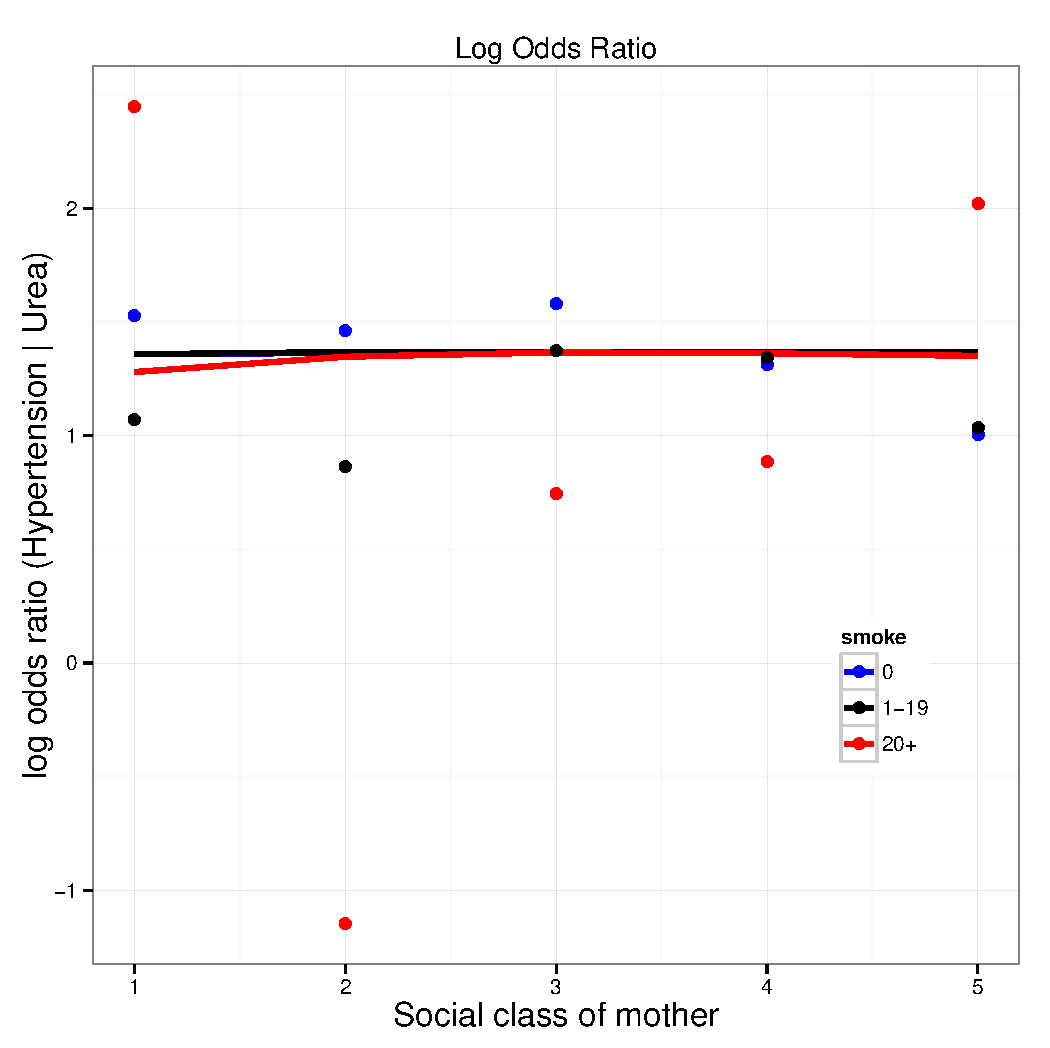
\includegraphics[width=.49\textwidth]{ch08/fig/tox-glm-logits3}
\caption{Observed (points) and fitted (lines) log odds ratios for the \data{Toxemia} data under Model 2.}
\label{fig:tox-glm-logits3}
\end{figure}

According to this model, \figref{fig:tox-glm-logits3} shows
that the fitted log odds ratio is in fact nearly constant,
while \figref{fig:tox-glm-logits1} shows that
the log odds for hypertension depends mainly on smoking
(with a large difference of the non-smoking mothers from the rest)
and that for protein urea depends mainly on social class.%
\footnote{
Some possible enhancements to these graphs include
\begin{seriate}
 \item plotting on the scale of probabilities or including a right vertical axis
 showing corresponding probabilities;
 \item using the same vertical axis limits for the two graphs for direct comparison.
\end{seriate}
}

Yet, the great variability of the observed points around the fitted
curves indicates that these relationships are not well-determined.
Adding error bars showing the standard error around each fitted point
would indicate that the data conforms as closely to the model as
can be expected, given the widely different sample sizes.
However, this would make the plots more complex, and so was omitted
here.
In addition to showing the pattern of the results according to the fitted
model, such graphs also help us to appreciate the model's limitations.


\end{Example}




\section{Chapter summary}\label{sec:loglin-summary}
\begin{itemize}
\item Polytomous responses may be handled in several ways as extensions of binary
logistic regression.  These methods require different fitting functions in \R,
however the graphical methods for plotting results are relatively straight-forward
extensions of those used for binary responses.
%\begin{seriate}
 \item The \emph{proportional odds model} (\secref{sec:ordinal}) is simple and convenient, but its validity
depends
on an assumption of equal slopes for adjacent-category logits.
 \item \emph{Nested dichotomies} (\secref{sec:nested}) among the response categories give a set of statistically independent, binary logistic submodels.
These may be regarded as a single, combined model for the polytomous response.
 \item \emph{Generalized logit models} (\secref{sec:genlogit}) provide the most general approach. These
 may be used to construct submodels comparing any pair of categories.
%\end{seriate}

\end{itemize}


\section{Further reading}\label{sec:loglin-reading}

\section{Lab exercises}\label{sec:loglin-lab}

\begin{Exercises}

  \exercise \exref{ex:vision-glm} presented an analysis of the data on visual acuity 
  for the subset of women in the \data{VisualAcuity} data.  Carry out a parallel
  analysis of the models fit there for the \code{men} in this data set, given by:
\begin{knitrout}
\definecolor{shadecolor}{rgb}{1, 0.961, 0.933}\color{fgcolor}\begin{kframe}
\begin{alltt}
\hlkwd{data}\hlstd{(}\hlstr{"VisualAcuity"}\hlstd{,} \hlkwc{package}\hlstd{=}\hlstr{"vcd"}\hlstd{)}
\hlstd{men} \hlkwb{<-} \hlkwd{subset}\hlstd{(VisualAcuity, gender}\hlopt{==}\hlstr{"male"}\hlstd{,} \hlkwc{select}\hlstd{=}\hlopt{-}\hlstd{gender)}
\end{alltt}
\end{kframe}
\end{knitrout}


  \exercise \tabref{tab:birthcontrol} gives a $4 \times 4$ table of opinions about
  premarital sex and whether methods of birth control should be made available
  to teenagers aged 14--16 from the 1991 General Social Survey
  \citep[Table 10.3]{Agresti:2013}.  Both variables are ordinal, and their
  grades are represented by the case of the row and column labels.
% latex table generated in R 3.0.1 by xtable 1.7-3 package
% Fri May 30 13:50:07 2014
\begin{table}[ht]
\centering
\caption{Opinions about premarital sex and availability of teenage birth control. 
  \emph{Source}: \citet[Table 10.3]{Agresti:2013}}
\label{tab:birthcontrol}
\begin{tabular}{rrrrr}
  \hline
  Premarital sex & \multicolumn{4}{c}{Birth control} \\
                 & DISAGREE & disagree & agree & AGREE \\ 
  \hline
  WRONG & 81 & 68 & 60 & 38 \\ 
  Wrong & 24 & 26 & 29 & 14 \\ 
  wrong & 18 & 41 & 74 & 42 \\ 
  OK & 36 & 57 & 161 & 157 \\ 
   \hline
\end{tabular}
\end{table} 


  \begin{enumerate*}
    \item Fit the independence model to these data using \func{loglm} or \func{glm}.
    \item Make a mosaic display showing departure from independence and describe
    verbally the pattern of association.
    \item Treating the categories as equally spaced, fit the $L \times L$ model
    of uniform association, as in \secref{sec:loglin-ordinal}.  Test the
    difference against the independence model with a \LR test.
    \item Fit the RC(1) model with \func{gnm}, and test the difference of
    this against the model of uniform association.
    \item Write a brief summary of these results, including plots useful
    for explaining the relationships in this data set.
  \end{enumerate*}
  
  \exercise The data set \data{gss8590} in \pkg{logmult} gives a $4 \times 5 \times 4$
  table of education levels and occupational categories for the four combinations
  of gender and race from the General Social Surveys, 1985--1990 as reported by
  \citet[Table 2]{Wong:2001}. \citet[Table 2.3B]{Wong:2010} later used the
  subset pertaining to women to illustrate RC(2) models.  This data is
  created below as \code{Women.tab}, correcting an inconsistency to conform with
  the 2010 table.
  

\begin{knitrout}
\definecolor{shadecolor}{rgb}{1, 0.961, 0.933}\color{fgcolor}\begin{kframe}
\begin{alltt}
\hlkwd{data}\hlstd{(gss8590,} \hlkwc{package}\hlstd{=}\hlstr{"logmult"}\hlstd{)}
\hlstd{Women.tab} \hlkwb{<-} \hlkwd{margin.table}\hlstd{(gss8590[,,}\hlkwd{c}\hlstd{(}\hlstr{"White Women"}\hlstd{,} \hlstr{"Black Women"}\hlstd{)],} \hlnum{1}\hlopt{:}\hlnum{2}\hlstd{)}
\hlstd{Women.tab[}\hlnum{2}\hlstd{,}\hlnum{4}\hlstd{]} \hlkwb{<-} \hlnum{49}
\hlkwd{colnames}\hlstd{(Women.tab)[}\hlnum{5}\hlstd{]} \hlkwb{<-} \hlstr{"Farm"}
\end{alltt}
\end{kframe}
\end{knitrout}
  \begin{enumerate*}
    \item Fit the independence model, and also the RC(1) and RC(2) models using
    \func{rc} with marginal weights, as illustrated in \exref{ex:mental6}.
    Summarize these statistical tests in a table.
    \item Plot the solution for the RC(2) model with 68\% confidence ellipses.
    What verbal labels would you use for the two dimensions?
    \item Is there any indication that a simpler model, using integer scores for
    the row (Education) or column (Occupation) categories or both might suffice?
    If so, fit the analogous column effects, row effects or $L \times L$ model,
    and compare with the models fit in part (a).
  \end{enumerate*}


\end{Exercises}
\begin{knitrout}\footnotesize
\definecolor{shadecolor}{rgb}{1, 0.961, 0.933}\color{fgcolor}\begin{kframe}
\begin{alltt}
\hlkwd{detach}\hlstd{(package}\hlopt{:}\hlstd{corrplot)}
\end{alltt}


{\ttfamily\noindent\bfseries\color{errorcolor}{\#\# Error in detach(package:corrplot): invalid 'name' argument}}\begin{alltt}
\hlkwd{detach}\hlstd{(package}\hlopt{:}\hlstd{VGAM)}
\hlcom{#detach(package:logmult)}
\hlcom{#remove(list=objects(pattern="\textbackslash{}\textbackslash{}.tab|\textbackslash{}\textbackslash{}.df|\textbackslash{}\textbackslash{}.fit"))}
\hlstd{.locals}\hlopt{$}\hlstd{ch08} \hlkwb{<-} \hlkwd{setdiff}\hlstd{(}\hlkwd{ls}\hlstd{(), .globals)}
\hlcom{#.locals$ch08}
\hlcom{#remove(list=.locals$ch08[sapply(.locals$ch03,function(n)\{!is.function(get(n))\})])}
\end{alltt}
\end{kframe}
\end{knitrout}


% <<ch9, child='ch09.Rnw'>>=
% @

%%%%%%%%%%%%%%%%%%%%%%%%%%%%%%%%%%%%%%%%%%%%%%%%%%%%%%%%%%%%%%%%%%%%%%%%%


% To resolve citations in the chapter, ...
{\itemsep -1pt
\bibliography{graphics,statistics,timeref,Rpackages}
%%% Use aux2bib to process the .aux file, creating references.bib
%%% Then change to line below
%\bibliography{references}
}

% \newpage
% This document was produced using:
% 
% <<session-info>>=
% print(sessionInfo(), locale = FALSE)
% @

	
%%%%% THE END %%%%%
\end{document}

